%!TEX TS-program = xelatex
%!TEX encoding = UTF-8 Unicode
\documentclass[a4paper, 12pt, oneside]{book}

\usepackage{cite}
%\usepackage{chapterbib}
%The chapterbib package facilitates multiple bibliographies in a LATEX document
\usepackage[hyphens]{url}
%Verbatim with URL-sensitive line breaks.
\usepackage[colorlinks=true,linkcolor=black,citecolor=black,filecolor=blue,urlcolor=blue,unicode]{hyperref}
%The hyperref package is used to handle cross-referencing commands in LaTeX to produce hypertext links in the document. The package provides backends for the \special set defined for HyperTeX DVI processors; for embedded pdfmark commands for processing by Acrobat Distiller (dvips and Y&Y’s dvipsone); for Y&Y’s dviwindo; for PDF control within pdfTeX and dvipdfm; for TeX4ht; and for VTeX’s pdf and HTML backends.
\usepackage{verbatim}
%The verbatim environment  simply reproduces every character you input, including all  s p a c e s!
\usepackage{color}
%you can set the color of the font of the text, and set the background color of the page.
\usepackage[dvipsnames]{xcolor}
%xecolor package is a simple package which defines about 140 different colors by XeTeX's font
\usepackage{graphicx}
%Standard LaTeX graphics.
\usepackage{array}
%The array environment is used to make a table of information, with column alignment (left, center, or right) and optional vertical lines separating the columns.
\usepackage{gensymb}
%Provides generic commands \degree, \celsius, \perthousand, \micro and \ohm which work both in text and maths mode.
\usepackage{indentfirst}
%Make the first line of all sections etc., be indented by the usual paragraph indentation. This should work with all the standard document classes. This minimalist package is part of the "tools" bundle in the LaTeX required distribution.
\usepackage{algorithm}
\usepackage{algpseudocode}
%A suite of tools for typesetting algorithms in pseudo-code. The algorithmicx package provides many possibilities to customize the layout of algorithms. You can use one of the predefined layouts (pseudocode, pascal and c and others), with or without modifications, or you can define a completely new layout for your specific needs.
\usepackage{enumitem}
%Control layout of itemize, enumerate, description.  It supersedes both enumerate and mdwlist (providing well- structured replacements for all their funtionality), and in addition provides functions to compute the layout of labels, and to 'clone' the standard environments, to create new environments with counters of their own.
\usepackage{mfirstuc}
%\makefirstuc{〈stuff 〉} This makes the first object of 〈stuff 〉 uppercase unless 〈stuff 〉 starts with a con- trol sequence followed by a non-empty group, in which case the first object in the group is converted to uppercase.
\usepackage{fancyvrb}
%This package provides very sophisticated facilities for reading and writing ver- batim TEX code.
\usepackage{amsfonts}
%TeX fonts from the American Mathematical Society.
\usepackage{ifmtarg}
%If-then-else command for processing potentially empty arguments.
\usepackage{amsmath}
%The amsmath package is a LATEX package that provides miscellaneous enhance- ments for improving the information structure and printed output of documents that contain mathematical formulas.
\usepackage{amssymb}
% Math symbols
\usepackage[mathcal]{euscript}
%This file sets up some font shape definitions to use the Euler script symbols in math mode.
\usepackage[notbib]{tocbibind}
%Add (or disable) bibliography/index/contents to Table of Contents.
\usepackage{rotating}
%Rotation tools, including rotated full-page floats.
\usepackage{hhline}
%The command \hhline produces a line like \hline, or a double line like \hline\hline, except for its interaction with vertical lines. The command takes a preamble (rather like the preamble of a tabular environment), and this specifies whether there are to be one or two horizontal lines, and what happens when the horizontal line meets a vertical one. The package is part of the tools bundle in the LaTeX required distribution.
\usepackage{wallpaper}
%Easy addition of wallpapers (background images) to LaTeX documents, including tiling.
\usepackage{pdfpages}
%Include PDF documents in LaTeX.
\usepackage{pst-fractal,pst-exa}
% The package will draw the Julia and Mandelbrot sets, the Sierpinski triangle, Koch flake, and Apollonius Circle as well as fractal trees (which need not be balanced) with a variety of different parameters (including varying numbers of iterations).

%Define \XeTeX \XeLaTeX command
\def\reflect#1{{\setbox0=\hbox{#1}\rlap{\kern0.5\wd0
 \special{x:gsave}\special{x:scale -1 1}}\box0 \special{x:grestore}}}
\def\XeLaTeX{\leavevmode
 \setbox0=\hbox{X\lower.5ex\hbox{\kern-.15em\reflect{E}}\kern-.08em\LaTeX}%
 \dp0=0pt\ht0=0pt\box0}
 \def\XeTeX{\leavevmode
 \setbox0=\hbox{X\lower.5ex\hbox{\kern-.15em\reflect{E}}\kern-.08em\TeX}%
 \dp0=0pt\ht0=0pt\box0}

% \usepackage[none]{hyphenat}  %hyphenation package

% Start Declare physics symbols
\newcommand{\gv}[1]{\ensuremath{\mbox{\boldmath$ #1 $}}} 
\newcommand{\grad}[1]{\gv{\nabla} #1} % for gradient
\let\divsymb=\div % rename builtin command \div to \divsymb
\renewcommand{\div}[1]{\gv{\nabla} \cdot #1} % for divergence
\newcommand{\curl}[1]{\gv{\nabla} \times #1} % for curl
\let\baraccent=\= % rename builtin command \= to \baraccent
\renewcommand{\=}[1]{\stackrel{#1}{=}} % for putting numbers above =
%end Declare

\usepackage{tabularx}
%tabularx, is defined, which takes the same arguments as tabular*, but modifies the widths of certain columns, rather than the inter column space, to set a table with the requested total width. The columns that may stretch are marked with the new token X in the preamble argument. This package requires the array package. The package is part of the tools bundle in the LaTeX required distribution.
\usepackage{lmodern}
%The Latin Modern family of fonts consists of 72 text fonts and 20 mathematics fonts, and is based on the Computer Modern fonts released into public domain by AMS (copyright © 1997 AMS).
\font\lmr="[lmroman10-regular]"

\usepackage{listings}
%Typeset source code listings using LaTeX.
\usepackage{textcomp}
%provide many text symbols (such as baht, bullet, copyright, musicalnote, onequarter, section, and yen)

\usepackage{amsthm}
%The package facilitates the kind of theorem setup typically needed in American Mathematical Society publications. The package offers the theorem setup of the AMS document classes (amsart, amsbook, etc.) encapsulated in LaTeX package form so that it can be used with other document classes. Amsthm is part of the (required) AMS-LaTeX distribution, so should be present in any LaTeX distribution.
\newtheorem{mydef-no-caption}{Definition}
\newenvironment{mydef}[1][]%
	{\begin{mydef-no-caption}{\ifnotmtarg{#1}{\textnormal{(\textbf{#1})}~}}}%
	{\end{mydef-no-caption}}

\usepackage{numprint}
%Print numbers with separators and exponent if necessary.
\npthousandsep{,}
\npthousandthpartsep{}
\npdecimalsign{.}

\usepackage{multirow}
%Create tabular cells spanning multiple rows.

\usepackage{ntu}
%NTU thesis style file
\hypersetup{
	pdfauthor={\authorEN{}},
	pdftitle={\titleEN{}},
	pdfsubject={NTU Thesis}
}

\usepackage{setspace}
%Set space between lines.

\usepackage[absolute]{textpos}
%Place boxes at arbitrary positions on the LaTeX page.
\lstdefinestyle{nonumbers}{numbers=none}
\textblockorigin{0mm}{0mm}

\setcounter{tocdepth}{2}

\pagestyle{plain}

\begin{document}

%----------- hyphenation  -----------
%\righthyphenmin=10  % Best hyphenation parameter

%----------- watermark -----------
%\CenterWallPaper{0.365}{watermark.pdf}

%----------- cover page -----------
\maketitle

%----------- side page, used for printing on spline -----------
\makeside


\frontmatter
%----------- generate the certification page by LaTeX -----------
%\makecertification
%----------- includepdf by using package pdfpages -----------
%\addcontentsline{toc}{chapter}{口試委員會審定書}
%
\includepdf[pages={1}]{cert.pdf}

\onehalfspacing
%\begin{acknowledgementsCH}
 這裡將簡單介紹如何利用\LaTeX\ 來編輯你的畢業論文,若不知道\LaTeX\ 是什麼或是沒有概念的話,建議你可以簡單看過放在此資料夾裡的\href{run:./latex123.pdf}{李果正-大家來學\LaTeX}前四章內容,在下載適合的\LaTeX\ 整合發行套件之後(請看第~\ref{it:download}項),可以嘗試用剛安裝好的\LaTeX\ 編輯器來編譯\href{run:./thesis.tex}{thesis.tex}這份文件,編譯的方法可以看下面第~\ref{it:comp}項的介紹,若編譯成功,所編譯出來的thesis.pdf文件的應該會跟此demo.pdf文件一模一樣,而且沒有任何問號符號,走到這一步的話,就差不多可以開始邊學習\LaTeX\ 邊編輯你的畢業論文了!基本上會使用到的指令都包含在論文的的各章節裡,怎麼在論文裡寫公式或是放圖之類的就自行看tex檔學吧。如果有任何問題或建議可以來信與我討論,我的信箱是\href{mailto:dran31545@gmail.com}{dran31545@gmail.com},或是到此範本\href{http://code.google.com/p/ntu-thesis-latex-template/}{Google Project}裡面的\href{http://code.google.com/p/ntu-thesis-latex-template/issues/list}{Issues}貼上你的問題與建議,我會盡我所能更新此範本,也歡迎大家自行重製、改良此範本並散布給他人,祝大家順利畢業!\\\\
 要編輯致謝請打開\href{run:./acknowledgementsCH.tex}{acknowledgementsCH.tex}\\
 \begin{enumerate}[leftmargin=0pt, topsep=0pt, itemsep=0pt, label=\Roman{*}.]
\item 此範本參考並修改自下列網站的資料:
\begin{enumerate}[topsep=0pt, itemsep=0pt, label=$\bullet$]
    \item \href{http://www.csie.ntu.edu.tw/~tzhuan/www/resources/ntu/}{如何用 LaTeX 排版臺灣大學碩士論文}\\
    \textemdash 台灣大學論文\LaTeX\ 樣版原創者\href{http://www.csie.ntu.edu.tw/~tzhuan/www/}{黃子桓}的教學網頁
    \item \href{http://www.hitripod.com/blog/2012/05/latex-thesis-template-quick-reference/}{LaTeX 常用語法及論文範本}\\
    \textemdash \href{http://www.hitripod.com/blog/}{Hitripod}所修改的範本,這裡參考了許多他所寫的格式和內容
    \item \href{http://www.cc.ntu.edu.tw/chinese/epaper/0014/20100920_1404.htm}{使用LaTeX做出精美的論文}
    \item \href{http://www.hitripod.com/blog/2011/04/xetex-chinese-font-cjk-latex/}{XeTeX:解決 LaTeX 惱人的中文字型問題}
    \item \href{http://code.google.com/p/ntuthesis/}{台灣大學碩士、博士論文的Latex模板}\\
\end{enumerate}
\item 幾個有用的參考資料及網路資源:
\begin{enumerate}[topsep=0pt, itemsep=0pt, label=$\bullet$]
    \item \href{run:./latex123.pdf}{李果正-大家來學\LaTeX}\textemdash 建議先看完前四章
    \item \href{http://en.wikibooks.org/wiki/LaTeX}{WIKIBOOKS-\LaTeX}\textemdash 好用的線上工具書
    \item \href{run:./Working_with_a_bib_file_using_Jabref.pdf}{Working with a .bib file using JabRef}
    \item \href{run:./Fi087_S.pdf}{Using BibDesk - A short tutorial}
    \item \href{http://www.dfcd.net/articles/latex/latex.html}{LaTeX for Physicists}\\
\end{enumerate}
\item 下載\LaTeX\ 整合發行套件,可參考\href{http://www.tug.org/texcollection/}{TeX Collection}:\label{it:download}
 \begin{enumerate}[topsep=0pt, itemsep=0pt, label=\arabic{*}.]
     \item \href{http://www.tug.org/mactex/}{MacTeX}: For \textcolor{Green}{\textbf{MacOSX}},下載\href{http://mirror.ctan.org/systems/mac/mactex/MacTeX.pkg}{MacTeX.pkg}
     \item \href{http://www.tug.org/protext/}{ProTeXt}: For \textcolor{Green}{\textbf{Windows}},下載\href{ftp://ftp.fernuni-hagen.de/pub/windows/win32/ProTeXt/}{ISO file}
     \item \href{http://www.tug.org/texlive/}{TeX Live}: For \textcolor{Green}{\textbf{GNU/Linux}} and \textcolor{Green}{\textbf{MacOSX}}, and \textcolor{Green}{\textbf{Windows}},下載\href{http://www.tug.org/texlive/acquire-iso.html}{ISO file}
     \item \href{http://ctan.org/}{CTAN}: The Comprehensive TeX Archive Network.\\
 \end{enumerate}

\item 好用的程式:
 \begin{enumerate}[topsep=0pt, itemsep=0pt, label=$\bullet$]
    \item 文獻管理系統:
        \begin{enumerate}[topsep=0pt, itemsep=0pt, label=\arabic{*}.]
         \item \href{http://jabref.sourceforge.net/}{JabRef}\\
                     可參考\href{run:./Working_with_a_bib_file_using_Jabref.pdf}{Working with a .bib file using JabRef}或是\href{https://www.google.com/search?q=jabref}{Google}及\href{http://www.youtube.com/results?search_query=jabref}{YouTube}
         \item \href{http://bibdesk.sourceforge.net/}{BibDesk} (For Mac)\\
                     可參考\href{run:./Fi087_S.pdf}{Using BibDesk - A short tutorial}或是\href{https://www.google.com/search?q=bibdesk}{Google}及\href{http://www.youtube.com/results?search_query=bibdesk}{YouTube}
         \end{enumerate}
         \item 方程式編輯器:\href{https://chrome.google.com/webstore/detail/dinfmiceliiomokeofbocegmacmagjhe?hl=zh-TW}{Daum Equation Editor} (Chrome App,必須使用Google瀏覽器)\\
 \end{enumerate} 
\item 編譯流程:\label{it:comp}
\begin{enumerate}[topsep=0pt, itemsep=0pt, label=\arabic{*}.]
    \item \texttt{xelatex thesis}\\ 對thesis.tex進行第一次XeLaTeX編譯,產生thesis.pdf以其他檔案
    \item \texttt{bibtex thesis}\\ 對thesis.tex進行BibTeX編譯,產生bbl檔以及blg檔
    \item \texttt{xelatex thesis}\\ 對thesis.tex進行第二次XeLaTeX編譯,產生目錄、圖表連結及參考文獻
    \item \texttt{xelatex thesis}\\ 對thesis.tex進行第三次XeLaTeX編譯,產生參考文獻連結,完成編譯
\end{enumerate} 
    \textcolor{Red}{注意!}此範本使用cite套件,可依據你利用文獻管理系統所整理好的\href{run:./thesisbib.bib}{thesisbib.bib}檔在論文最後產生參考文獻頁面,若你的系所規定要在每個章節的後面產生參考文獻,則可以用chapterbib套件,來對每個有附參考文獻的章節tex檔進行一次BibTeX編譯產生bbl檔,如範例的\href{run:./introduction.tex}{introduction.tex}、\href{run:./THM.tex}{THM.tex}和\href{run:./EXP.tex}{EXP.tex},如果有這需要請把\href{run:./thesis.tex}{thesis.tex}檔裡使用cite套件的指令利用註解符號\texttt{\%}來取消使用cite套件,並刪去出現在使用chapterbib套件指令前面的註解符號\texttt{\%}來啟動使用chapterbib套件
    \begin{verbatim}
\usepackage{cite}
%\usepackage{chapterbib}
改成
%\usepackage{cite}
\usepackage{chapterbib}
    \end{verbatim}
    再來利用註解符號\texttt{\%}取消會把參考文獻放在論文最後的指令
    \begin{verbatim}
\bibliographystyle{unsrt}
\addcontentsline{toc}{chapter}{\bibname}
\bibliography{thesisbib}
改成
%\bibliographystyle{unsrt}
%\addcontentsline{toc}{chapter}{\bibname}
%\bibliography{thesisbib}
    \end{verbatim}
    再把用來輸入章節檔案的\texttt{\textbackslash input}指令改成\texttt{\textbackslash include}指令
     \begin{verbatim}
\chapter{Introduction}
\label{c:intro}

There can be million lines of code in today's software system.
On such a scale of complexity, defects in the source codes are unavoidable.  
Various empirical studies show that the defect density of commercial software system is around 1 to 20 defects in every 1000 lines of source code\cite{Sommerville:2006:SE:1196763}.
Therefore, developers of systems created many engineering techniques to contain the damage that could be caused by such defects.
For example, a software system may have several measures to its disposal to avoid system failure, including resending the request, resetting the server, clearing the communication buffers, and etc when observing that a critical service request is not acknowledged.
However, in general, since all the recovery cost time and money it is important to estimate how to organize the measures for the maximal resilience of the system against realistic errors.
At the moment, an automated support which can suggest defence techniques to development teams is missing.
I created a game theoretic approach to study this problem and carried out experiments to show how this approach can be helpful in  synthesizing the most resilient defence of software systems against multiple errors.

The naive way to measure the safety level of a system is to find the number of errors that it can endure before running into failure state.
But in second thought, no non-trivial system can handle unlimited errors without degrading to inevitable system failure.
Thus, it would be meaningless to analyse the resilience level of the systems to software errors can proceed without creating a realistic error model in which practical control mechanism can be devised to defend the systems against errors.
In this work, I am interested in defending the system against a more restricted error model, but still let the error model has a quantifiable level of power in order to simulate different error scenarios.
Further more, I think a reasonable foundation need to take into consider that the life-time of a software system is much longer than the duration needed for a reasonably designed software system to recover from an error.
Therefore, I propose to evaluate control mechanism of software systems on how many errors the control can endure before recovery to safe states.
I then present an algorithm to find a control strategy that can handle the maximum number of such errors.

Let us standardize the basic terms before proceeding further.
A design defect in software or hardware is called a {\it fault} in embedded systems.
An {\it error} (sometimes called component failure in the literature) is the effect of a fault that causes a difference between the expected and the actual behavior of a software system, e.g., measurement errors, read/write errors, etc. 
An {\it error} does not always lead to a system failure, but may instead be repaired by, e.g., a defence mechanism in the software. 
That is, an {\it error} may be detected and fixed/neutralized before it creates any harm to the system or its users.
A {\it failure} is the fact that users can observe the faulty behavior created by {\it errors}.

My specific goal is to develop a technique for finding a control mechanism of a software system which can against the maximal number of dense errors without degrading to failure.
My inspiration is from methods for resilient avionic systems\cite{conf/ftrtft/Rushby92}, where fault tolerance is designed to recover from a bounded number of errors.
The number of errors a system needs to tolerate is calculated from the mean time between errors of individual components and the maximal duration of the system.
I use the quality guarantees one obtains for an airplain(the system) as an example to demonstrate the difference between the objective to tolerate up to {\it k errors} and sequences of separated blocks of up to {\it k dense errors} in a short period.
Assuming the operating time of the system is 20 hours, the mean time between exponentially distributed errors is 10 hours and the repair time is 3.6 seconds.
The mean time between dense errors (consecutive errors before system recovery) is calculated in Table~\ref{tab.mtbf}.
\begin{table*}
\begin{center}
\begin{tabular}{l||c|c|c|c|c|c|c|c}\hline 
$k$              & $0$     & $1$     &    $2$   &  $3$  & $4$ & $5$ & $6$ & $\ldots$ \\\hline 
$k$ errors       & $0.865$ & $0.594$ & $0.333$ & $0.143$ & $0.053$ & $0.017$ & $0.005$ & $\ldots$ \\
$k$ dense errors & $0.865$ & $2 \cdot 10^{-4}$ & $2 \cdot 10^{-9}$ & $2 \cdot 10^{-14}$ & $2\cdot 10^{-19}$ & $2\cdot 10^{-24}$ & $2\cdot 10^{-29}$ & $\ldots$ 
\\ \hline 
\end{tabular}
\end{center}
\caption{Probabilities of $k$ dense errors} 
\label{tab.mtbf} 
\end{table*} 
%\bibliographystyle{unsrt}
%\bibliography{thesisbib}
The figures for $k$ errors (component failures) are simply the values 
for the Poisson distribution with coefficient $2$.
To explain the figures for $k$ dense errors, 
consider the density of 2 dense errors occurring in close succession.
If an error occurs, the chance that the next error occurs 
within the repair time (3.6 seconds) is approximately $\frac{1}{10000}$.
The goal to tolerate an arbitrary number of up to $k$-dense errors is, of course, 
much harder than the goal of tolerating up to $k$ errors, but, 
as the example shows, the number $k$ can be much smaller.   
Tolerating an arbitrary number of errors 
(with a distance of at least $3.6$ seconds between them) 
creates the same likelihood to result in a system failure 
as tolerating up to $9$ errors overall, and 
tolerating up to $15$ errors still results 
in a $70\%$ higher likelihood of a system failure 
than tolerating blocks of up to $2$ errors in this example. 
Only errors for which this is the case could cause a system failure.
The mean time between blocks of two dense errors is therefore not ten hours, 
but 100,000\label{reply2.100000} hours.
Likewise, it increases to 1,000,000,000 (one billion) hours for blocks of three dense errors, and so forth.

Maximizing the number of dense errors that are permitted before full recovery 
is therefore a natural design goal.  
After full recovery, the system is allowed again the same number of errors.
Now, if the {\em mean time between errors} ({\em MTBE}) 
is huge compared to the time the system needs to fully recover, 
then the mean time between system failures (MTBF) grows immensely. 

We view the problem of designing a resilient control mechanism 
towards dense errors as a two-player game, 
called {\em safety resilience game}, 
between the system (\label{reply1.protagonist.player1}protagonist\footnote{In game theory, a protagonist sometimes is also called {\em player 1}.}, `he' for convenience) 
and a hostile agent (antagonist\footnote{In game theory, an antagonist sometimes is also called {\em player 2}.}, `she' for convenience) 
that injects errors into the system under execution.\label{reply1.antagonist.inject.errors}   
The protagonist wants to keep the system from failure in the presence of errors, 
while the antagonist wants to derail the system to failure. 
\label{reply1.how.models} 
Specifically, 
system designers may model their system, defense mechanism, and error model 
as a finite game graph.  
The nodes in the graph represent system states.
These system states are partitioned into three classes:
the safe states, the failure states, and the recovery states. 
Some transitions are labeled with errors while others are considered normal transitions.  
The game is played with respect to a resilience level $k$.  
If a play ever enters a failure state, then the antagonist wins in the play.  
Otherwise, the protagonist wins.

The protagonists plays by selecting a move, intuitively the `normal' event that should happen next (unless an error is injected).
The antagonist can then decide to trigger 
an error transition (injecting an error) with the intention to
eventually deflect the system into a failure state. 
Our error model, however, restricts 
the antagonist to inject at most $k$ errors before she allows for a long period of time that the system may use to recover to the safe states.
(If the antagonist decides to use less than $k$ errors, the protagonist does not know about this.
It proves that this information is not required, as we will show
\label{reply1.memoryless.future} that the protagonist can play memoryless.)
After full recovery by the protagonist to the safe states, the antagonist is allowed again 
to inject the same number of errors, and so forth.
  
If the system can win this game, then the system is called {\em $k$-resilient}.
For $k$-resilient systems, there exists a control strategy---even one that does not use memory---to make the system 
resilient in the presence of blocks of up to $k$ dense errors. 
We argue that, if the component MTBF is huge compared to the time the system needs to fully recover, then the expected time for system breakdown grows immensely.  

Besides formally defining safety resilience games, we also present algorithms 
for answering the following questions.  
\label{reply2.alg.sfrch.res}
\begin{itemize} 
\item Given an integer $k$, a set $F$ of failure states, and 
  a set $S$ of safe states (disjoint from $F$), is there a recovery mechanism that 
  can endure up to $k$ dense errors, 
  effectively avoid entering $F$, and quickly direct the system back to $S$.  
  Sometimes, the system designers may have designated parts of the state space 
  for the recovery mechanism.  
  The answer to this question thus also implicitly tells 
  whether the recovery 
  mechanism is fully functional in the recovery process. 
\item Given an integer $k$ and the set of failure states, 
  what is the maximal set of safe states, 
  for which the system has a strategy to maintain $k$-resilience?
  In game theory, this means that 
  safety resilience games can be used for synthesizing safety regions 
  for a given bound on consecutive errors before the system is fully recovered.  
  
The question can be extended to not only partition the states into safety, recovery, and failure states, but also for providing memoryless control on the safety and recovery states.
  
\item Given a set of failure states, what is the maximal resilience level of the system that can be achieved with proper control?  
  We argue that this maximal resilience level is a well-defined and plausible indicator of 
  the defense strength of a control mechanism against a realistic error model. 
\end{itemize} 
With our technique, 
software engineers and system designers 
can focus on maximizing the number of dense errors that 
the system can tolerate infinitely often, providing that they are grouped into blocks that are separated by a short period of time, which is sufficient for recovery.

We investigate how to analyze the game with existing techniques. 
We present an extension to alternating-time $\mu$-calculus (AMC) 
and propose to use the AMC model-checking algorithm on concurrent games to check 
resilience levels of embedded systems. 
We present reduction from safety resilience games to 
AMC formulas and concurrent game structures.  
Then we present a PTIME algorithm for answering whether the system can be 
controlled to tolerate up to a given number of dense errors.  
The algorithm can then be used to find the maximal resilience level 
that can be achieved of the system. 
The evaluation is constructive:  
it provides a control strategy  
for the protagonist, which can be used to control a system 
to meet this predefined resilience level.  

  =>  \chapter{Introduction}
\label{c:intro}

There can be million lines of code in today's software system.
On such a scale of complexity, defects in the source codes are unavoidable.  
Various empirical studies show that the defect density of commercial software system is around 1 to 20 defects in every 1000 lines of source code\cite{Sommerville:2006:SE:1196763}.
Therefore, developers of systems created many engineering techniques to contain the damage that could be caused by such defects.
For example, a software system may have several measures to its disposal to avoid system failure, including resending the request, resetting the server, clearing the communication buffers, and etc when observing that a critical service request is not acknowledged.
However, in general, since all the recovery cost time and money it is important to estimate how to organize the measures for the maximal resilience of the system against realistic errors.
At the moment, an automated support which can suggest defence techniques to development teams is missing.
I created a game theoretic approach to study this problem and carried out experiments to show how this approach can be helpful in  synthesizing the most resilient defence of software systems against multiple errors.

The naive way to measure the safety level of a system is to find the number of errors that it can endure before running into failure state.
But in second thought, no non-trivial system can handle unlimited errors without degrading to inevitable system failure.
Thus, it would be meaningless to analyse the resilience level of the systems to software errors can proceed without creating a realistic error model in which practical control mechanism can be devised to defend the systems against errors.
In this work, I am interested in defending the system against a more restricted error model, but still let the error model has a quantifiable level of power in order to simulate different error scenarios.
Further more, I think a reasonable foundation need to take into consider that the life-time of a software system is much longer than the duration needed for a reasonably designed software system to recover from an error.
Therefore, I propose to evaluate control mechanism of software systems on how many errors the control can endure before recovery to safe states.
I then present an algorithm to find a control strategy that can handle the maximum number of such errors.

Let us standardize the basic terms before proceeding further.
A design defect in software or hardware is called a {\it fault} in embedded systems.
An {\it error} (sometimes called component failure in the literature) is the effect of a fault that causes a difference between the expected and the actual behavior of a software system, e.g., measurement errors, read/write errors, etc. 
An {\it error} does not always lead to a system failure, but may instead be repaired by, e.g., a defence mechanism in the software. 
That is, an {\it error} may be detected and fixed/neutralized before it creates any harm to the system or its users.
A {\it failure} is the fact that users can observe the faulty behavior created by {\it errors}.

My specific goal is to develop a technique for finding a control mechanism of a software system which can against the maximal number of dense errors without degrading to failure.
My inspiration is from methods for resilient avionic systems\cite{conf/ftrtft/Rushby92}, where fault tolerance is designed to recover from a bounded number of errors.
The number of errors a system needs to tolerate is calculated from the mean time between errors of individual components and the maximal duration of the system.
I use the quality guarantees one obtains for an airplain(the system) as an example to demonstrate the difference between the objective to tolerate up to {\it k errors} and sequences of separated blocks of up to {\it k dense errors} in a short period.
Assuming the operating time of the system is 20 hours, the mean time between exponentially distributed errors is 10 hours and the repair time is 3.6 seconds.
The mean time between dense errors (consecutive errors before system recovery) is calculated in Table~\ref{tab.mtbf}.
\begin{table*}
\begin{center}
\begin{tabular}{l||c|c|c|c|c|c|c|c}\hline 
$k$              & $0$     & $1$     &    $2$   &  $3$  & $4$ & $5$ & $6$ & $\ldots$ \\\hline 
$k$ errors       & $0.865$ & $0.594$ & $0.333$ & $0.143$ & $0.053$ & $0.017$ & $0.005$ & $\ldots$ \\
$k$ dense errors & $0.865$ & $2 \cdot 10^{-4}$ & $2 \cdot 10^{-9}$ & $2 \cdot 10^{-14}$ & $2\cdot 10^{-19}$ & $2\cdot 10^{-24}$ & $2\cdot 10^{-29}$ & $\ldots$ 
\\ \hline 
\end{tabular}
\end{center}
\caption{Probabilities of $k$ dense errors} 
\label{tab.mtbf} 
\end{table*} 
%\bibliographystyle{unsrt}
%\bibliography{thesisbib}
The figures for $k$ errors (component failures) are simply the values 
for the Poisson distribution with coefficient $2$.
To explain the figures for $k$ dense errors, 
consider the density of 2 dense errors occurring in close succession.
If an error occurs, the chance that the next error occurs 
within the repair time (3.6 seconds) is approximately $\frac{1}{10000}$.
The goal to tolerate an arbitrary number of up to $k$-dense errors is, of course, 
much harder than the goal of tolerating up to $k$ errors, but, 
as the example shows, the number $k$ can be much smaller.   
Tolerating an arbitrary number of errors 
(with a distance of at least $3.6$ seconds between them) 
creates the same likelihood to result in a system failure 
as tolerating up to $9$ errors overall, and 
tolerating up to $15$ errors still results 
in a $70\%$ higher likelihood of a system failure 
than tolerating blocks of up to $2$ errors in this example. 
Only errors for which this is the case could cause a system failure.
The mean time between blocks of two dense errors is therefore not ten hours, 
but 100,000\label{reply2.100000} hours.
Likewise, it increases to 1,000,000,000 (one billion) hours for blocks of three dense errors, and so forth.

Maximizing the number of dense errors that are permitted before full recovery 
is therefore a natural design goal.  
After full recovery, the system is allowed again the same number of errors.
Now, if the {\em mean time between errors} ({\em MTBE}) 
is huge compared to the time the system needs to fully recover, 
then the mean time between system failures (MTBF) grows immensely. 

We view the problem of designing a resilient control mechanism 
towards dense errors as a two-player game, 
called {\em safety resilience game}, 
between the system (\label{reply1.protagonist.player1}protagonist\footnote{In game theory, a protagonist sometimes is also called {\em player 1}.}, `he' for convenience) 
and a hostile agent (antagonist\footnote{In game theory, an antagonist sometimes is also called {\em player 2}.}, `she' for convenience) 
that injects errors into the system under execution.\label{reply1.antagonist.inject.errors}   
The protagonist wants to keep the system from failure in the presence of errors, 
while the antagonist wants to derail the system to failure. 
\label{reply1.how.models} 
Specifically, 
system designers may model their system, defense mechanism, and error model 
as a finite game graph.  
The nodes in the graph represent system states.
These system states are partitioned into three classes:
the safe states, the failure states, and the recovery states. 
Some transitions are labeled with errors while others are considered normal transitions.  
The game is played with respect to a resilience level $k$.  
If a play ever enters a failure state, then the antagonist wins in the play.  
Otherwise, the protagonist wins.

The protagonists plays by selecting a move, intuitively the `normal' event that should happen next (unless an error is injected).
The antagonist can then decide to trigger 
an error transition (injecting an error) with the intention to
eventually deflect the system into a failure state. 
Our error model, however, restricts 
the antagonist to inject at most $k$ errors before she allows for a long period of time that the system may use to recover to the safe states.
(If the antagonist decides to use less than $k$ errors, the protagonist does not know about this.
It proves that this information is not required, as we will show
\label{reply1.memoryless.future} that the protagonist can play memoryless.)
After full recovery by the protagonist to the safe states, the antagonist is allowed again 
to inject the same number of errors, and so forth.
  
If the system can win this game, then the system is called {\em $k$-resilient}.
For $k$-resilient systems, there exists a control strategy---even one that does not use memory---to make the system 
resilient in the presence of blocks of up to $k$ dense errors. 
We argue that, if the component MTBF is huge compared to the time the system needs to fully recover, then the expected time for system breakdown grows immensely.  

Besides formally defining safety resilience games, we also present algorithms 
for answering the following questions.  
\label{reply2.alg.sfrch.res}
\begin{itemize} 
\item Given an integer $k$, a set $F$ of failure states, and 
  a set $S$ of safe states (disjoint from $F$), is there a recovery mechanism that 
  can endure up to $k$ dense errors, 
  effectively avoid entering $F$, and quickly direct the system back to $S$.  
  Sometimes, the system designers may have designated parts of the state space 
  for the recovery mechanism.  
  The answer to this question thus also implicitly tells 
  whether the recovery 
  mechanism is fully functional in the recovery process. 
\item Given an integer $k$ and the set of failure states, 
  what is the maximal set of safe states, 
  for which the system has a strategy to maintain $k$-resilience?
  In game theory, this means that 
  safety resilience games can be used for synthesizing safety regions 
  for a given bound on consecutive errors before the system is fully recovered.  
  
The question can be extended to not only partition the states into safety, recovery, and failure states, but also for providing memoryless control on the safety and recovery states.
  
\item Given a set of failure states, what is the maximal resilience level of the system that can be achieved with proper control?  
  We argue that this maximal resilience level is a well-defined and plausible indicator of 
  the defense strength of a control mechanism against a realistic error model. 
\end{itemize} 
With our technique, 
software engineers and system designers 
can focus on maximizing the number of dense errors that 
the system can tolerate infinitely often, providing that they are grouped into blocks that are separated by a short period of time, which is sufficient for recovery.

We investigate how to analyze the game with existing techniques. 
We present an extension to alternating-time $\mu$-calculus (AMC) 
and propose to use the AMC model-checking algorithm on concurrent games to check 
resilience levels of embedded systems. 
We present reduction from safety resilience games to 
AMC formulas and concurrent game structures.  
Then we present a PTIME algorithm for answering whether the system can be 
controlled to tolerate up to a given number of dense errors.  
The algorithm can then be used to find the maximal resilience level 
that can be achieved of the system. 
The evaluation is constructive:  
it provides a control strategy  
for the protagonist, which can be used to control a system 
to meet this predefined resilience level.  


\chapter{Theory of surface plasmon polaritons in metallic nano-structures}
\label{c:thm}
\section{Definition of plasmon}

Plasmon is collective oscillation of conduction electron gas, a quasi-particle resulting from the quantization of plasma oscillations just like phonons are quantizations of mechanical vibrations. The simplest case is the volume plasmon as shown in Figure~\ref{fig:bulk}.
\begin{figure}[htb]
\centering
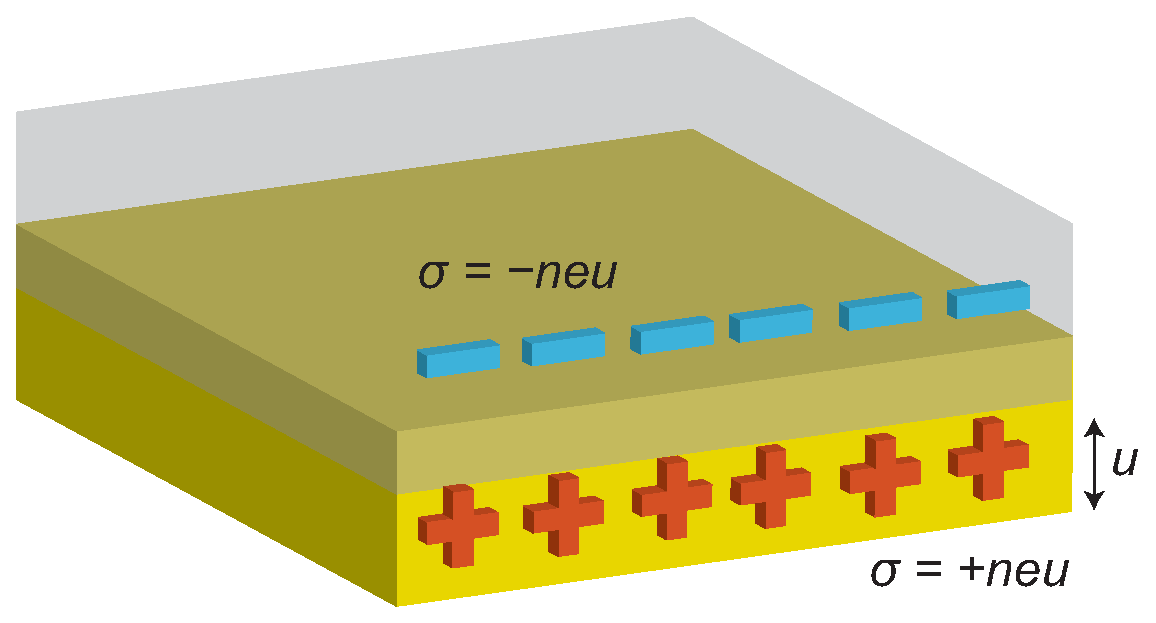
\includegraphics[scale=0.5]{THM/bulk.eps}
\caption{\label{fig:bulk}Longitudinal collective oscillations of the conduction electrons of a metal (Volume plasmons)}
\end{figure}
 We can derive plasma frequency $\omega_p$ from the simple harmonics oscillation model, a collective displacement of the electron cloud by a distance $u$ leads to a surface charge density $\sigma = \pm neu$ at the slab boundaries. This establishes a homogeneous electric field $\mathbf{E} = \frac{neu}{\varepsilon_0}$ inside the slab. Thus, the displaced electrons experience a restoring force, and their movement can be described by the equation of motion $nm\ddot{u} = -ne\mathbf{E}$. Inserting the expression for the electric field, this leads to
 \begin{subequations}
 \begin{align}
 nm\ddot{u} = -\frac{n^2e^2u}{\varepsilon_0} \\
 \ddot{u} + {\omega_p}^{2}u = 0\text{.}
 \end{align}
 \end{subequations}
  The plasma frequency $\omega_p = \sqrt{\frac{ne^2}{\varepsilon_0m}}$ can thus be recognized as the natural frequency of a free oscillation of the electron sea. The quanta of these charge oscillations are called plasmons. Due to the longitudinal nature of the excitation, volume plasmons do not couple to transverse electromagnetic waves, and can only be excited by particle impact. We can derive the dispersion relation of the generalization of volume plasmons, traveling plasma waves, from curl electric field equations (Equations~\ref{eq:curlE})
 \begin{subequations}
 \begin{align}
 \curl{\curl \mathbf{E}} &= -\mu_0 \frac{\partial^2\mathbf{D}}{\partial t^2}\label{eq:curlE}\\
\mathbf{K}( \mathbf{K}\cdot \mathbf{E}-K^{ 2 }\mathbf{E} ) &=-\varepsilon ( \mathbf{K},\omega  ) \frac { { \omega  }^{ 2 } }{ { c }^{ 2 } } \mathbf{E}
 \end{align}
 \end{subequations}  
and plasma model, and a simple equation of motion for an electron of the plasma subjected to an external electric field $\mathbf{E}$
 \begin{equation}
m\ddot{\mathbf{x}} + m\gamma\dot{\mathbf{x}} = -e\mathbf{E}\text{.}
\end{equation}
Assuming a harmonic time dependence $\mathbf{E}( t )=\mathbf{E}_0\mathrm{e}^{-i\omega t}$ of the driving field, a particular solution of this equation describing the oscillation of the electron is $\mathbf{x} ( t ) = \mathbf{x}_0 \mathrm{e}^{-i\omega t} $. The complex amplitude $\mathbf{x}_0$ incorporates any phase shifts between driving field and response via
\begin{equation}
\mathbf{x} ( t ) = \frac{e}{m( \omega^2 + i\gamma\omega )}\mathbf{E}( t )\text{.}
\end{equation}
The displaced electrons contribute to the macroscopic polarization
\begin{equation}
\mathbf{P}=-\frac{ne^2}{m( \omega^2 + i\gamma\omega )}\mathbf{E}( t )\text{.}
\end{equation}
Inserting $\mathbf{P}$ into dielectric displacement field equation $\mathbf{D} = \varepsilon_0\mathbf{E} + \mathbf{P}$ yields
\begin{equation}
\mathbf{D} = \varepsilon_0(1-\frac{\omega_p^2}{\omega^2 + i\gamma\omega})\mathbf{E}\text{,}
\end{equation}
where $\omega_p^2 = \frac{ne^2}{\varepsilon_0m}$. Therefore, the dielectric function of the free electron gas
\begin{equation}
\varepsilon(\omega) = 1- \frac{\omega_p^2}{\omega^2 + i\gamma\omega}\text{.}\label{eq:dielefu}
\end{equation}
We arrive at the desired result by using equation~\ref{eq:dielefu} and the generic dispersion relation $K^2=\varepsilon(\mathbf{K},\omega)\frac{\omega^2}{c^2}$, the dispersion relation of traveling waves becomes
\begin{equation}
\omega^2 = \omega_p^2 + \mathbf{K}^2c^2\text{.}
\end{equation}
From this relation, we can figure out the oscillation properties in any frequency of external field. Note that this branch can not confine the electromagnetic waves, it would radiate out the energy, so this mode is also called radiative surface plasmon.

\section{Surface plasmon polaritons at interface between dielectric and metal}

Surface plasmon polaritons (SPPs) are eigenmodes of transverse magnetic (TM) waves, which coupling the electromagnetic fields to oscillations of the conductor's electron plasma, propagate at a interface between dielectric and metal, and are confined in perpendicular direction. Providing a flat interface between dielectric and metal half-spaces with dielectric constants $\varepsilon_d$ and $\varepsilon_m$ , respectively, and assuming the interface normal to z direction and the SPPs propagate along the $x$ direction, the SPP wave vector $\beta$ is related to the frequency $\omega$ through the dispersion relation
\begin{equation}
\beta = k_0\sqrt{\frac{\varepsilon_d\varepsilon_m}{\varepsilon_d + \varepsilon_m}}\text{,}\label{eq:sppsdisp}
\end{equation}
where $k_0 = \omega/c$ is the free-space wave vector. We take $\omega$ to be real and allow $\beta$ to be complex.

The optical response of metals is often described by the Drude model for a free-electron gas~\cite{kittel1976introduction},
\begin{equation}
\varepsilon_{Drude}(\omega)=1-\frac{\omega_p^2}{\omega^2+i\Gamma\omega}\text{,}
\end{equation}
in which $\Gamma$ is a damping rate due to electron-electron and electron-phonon scattering.
Figure~\ref{fig:SPPdisp} shows the dispersion curve~\ref{eq:sppsdisp} with Drude metal  in the absence of losses ($\Gamma=0$) for air ($\varepsilon_d = 1$) and fused silica ($\varepsilon_d = 2.25$) interface.
\begin{figure}[htb]
\centering
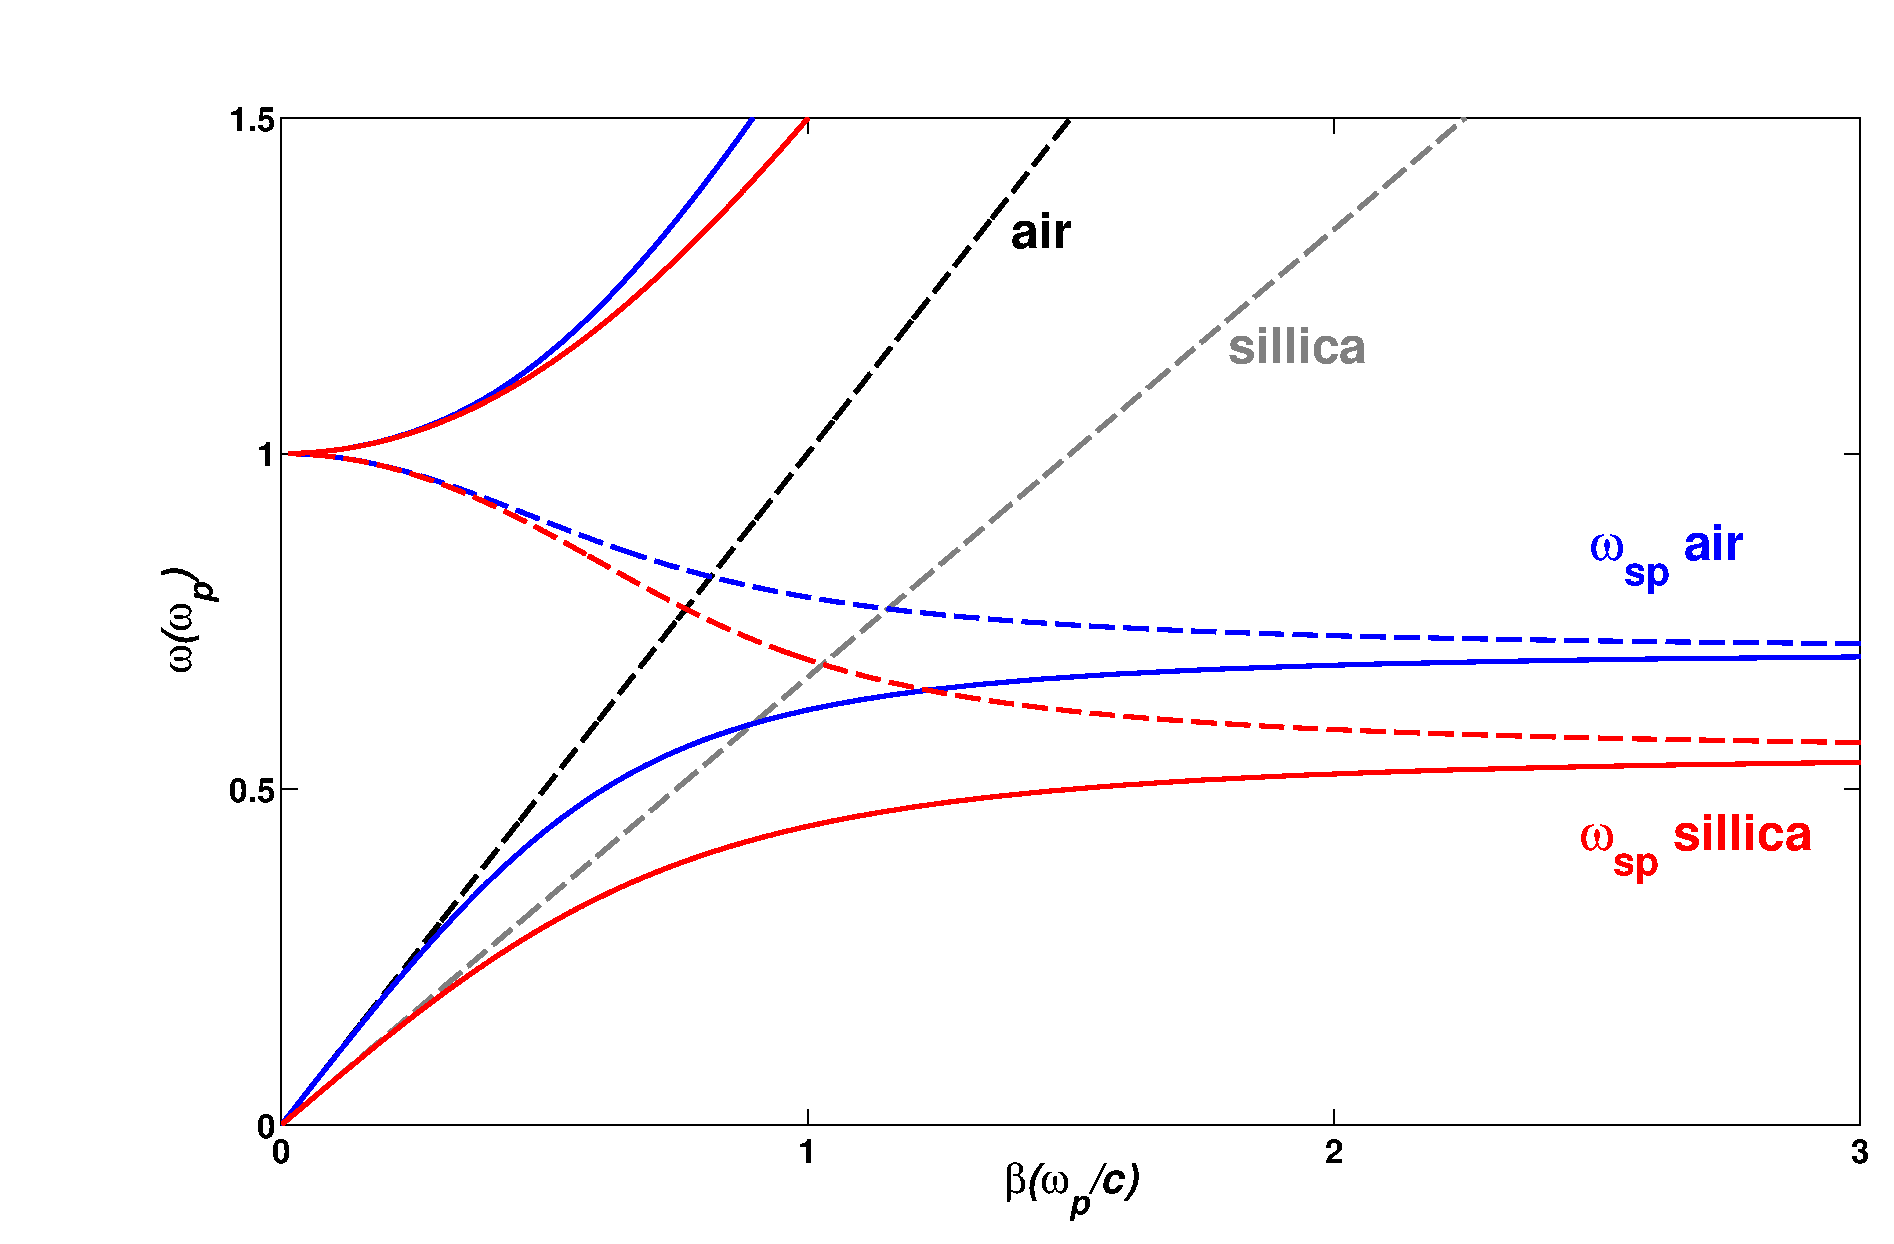
\includegraphics[scale=0.4]{THM/SPPdisp.eps}
\caption{\label{fig:SPPdisp}Dispersion relation of SPPs at the interface between a Drude metal with negligible collision frequency and air (blue curves) and silica (red curves).}
\end{figure}
For small wave vectors SPPs propagation constant $\beta$ is close to $k_0$ at the light line, in the opposite regime of the frequency close to surface plasmon frequency $\omega_p$. It also shows that the SPPs line lying to the right of the respective light lines of air and silica, so that SPPs are directed by light due to phase mismatching. The wave vector mismatch between SPPs and radiation modes needs to be overcome in order to excite or detect SPPs. This can be achieved by multiple methods~\cite{raether1988surface}. In the Otto configuration, light in a prism that is brought in close vicinity to a metal surface can excite SPPs through coupling to the evanescent field. Because light in the prism has a larger wave vector than that in air, it can be phase-matched to the SPPs. In the related Kretschmann-Raether geometry, coupling to SPPs occurs through a metal film that is deposited on a prism. In the grating coupling configuration, metal surface with a shallow grating of grooves or holes with lattice constant $a$. For the simple 1D grating of grooves depicted in Figure~\ref{fig:grating},
\begin{figure}[htb]
\centering
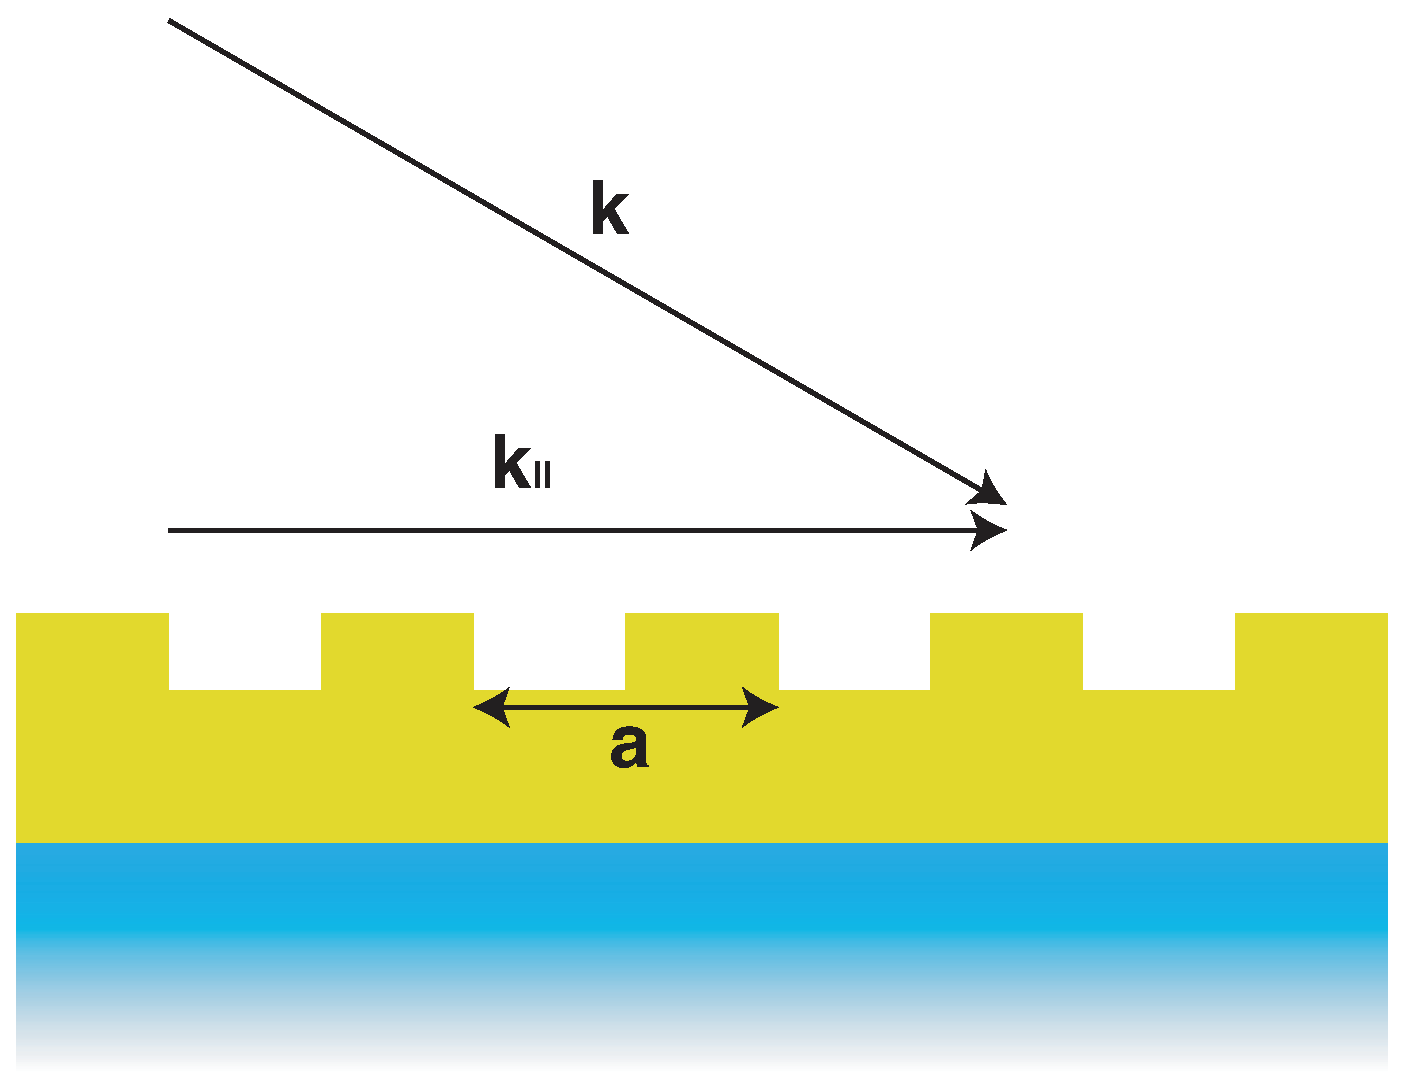
\includegraphics[scale=0.5]{THM/grating.eps}
\caption{\label{fig:grating}Phase-matching of light to SPPs the grating coupling configuration.}
\end{figure}
phase-matching takes place when the condition is fulfilled
\begin{equation}
\beta = k_0 \sin{\theta} \pm \nu g\text{,}
\end{equation}
where $g=\frac{2\pi}{a}$ is the reciprocal vector of the grating, and $\nu=(1,2,3\dots)$.
As with prism coupling, excitation of SPPs is detected as a minimum in the reflected light. The reverse process can also take place, SPPs propagating along a surface modulated with a grating can couple to light and thus radiate. 

%\bibliographystyle{unsrt}
%\bibliography{thesisbib}           =>  \chapter{Theory of surface plasmon polaritons in metallic nano-structures}
\label{c:thm}
\section{Definition of plasmon}

Plasmon is collective oscillation of conduction electron gas, a quasi-particle resulting from the quantization of plasma oscillations just like phonons are quantizations of mechanical vibrations. The simplest case is the volume plasmon as shown in Figure~\ref{fig:bulk}.
\begin{figure}[htb]
\centering
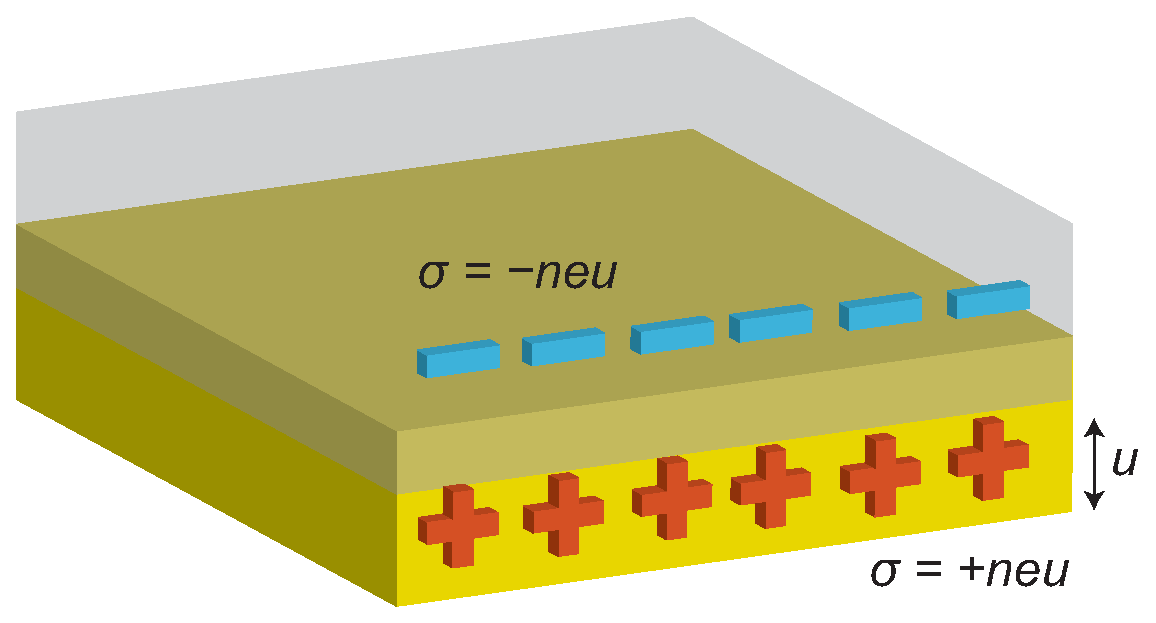
\includegraphics[scale=0.5]{THM/bulk.eps}
\caption{\label{fig:bulk}Longitudinal collective oscillations of the conduction electrons of a metal (Volume plasmons)}
\end{figure}
 We can derive plasma frequency $\omega_p$ from the simple harmonics oscillation model, a collective displacement of the electron cloud by a distance $u$ leads to a surface charge density $\sigma = \pm neu$ at the slab boundaries. This establishes a homogeneous electric field $\mathbf{E} = \frac{neu}{\varepsilon_0}$ inside the slab. Thus, the displaced electrons experience a restoring force, and their movement can be described by the equation of motion $nm\ddot{u} = -ne\mathbf{E}$. Inserting the expression for the electric field, this leads to
 \begin{subequations}
 \begin{align}
 nm\ddot{u} = -\frac{n^2e^2u}{\varepsilon_0} \\
 \ddot{u} + {\omega_p}^{2}u = 0\text{.}
 \end{align}
 \end{subequations}
  The plasma frequency $\omega_p = \sqrt{\frac{ne^2}{\varepsilon_0m}}$ can thus be recognized as the natural frequency of a free oscillation of the electron sea. The quanta of these charge oscillations are called plasmons. Due to the longitudinal nature of the excitation, volume plasmons do not couple to transverse electromagnetic waves, and can only be excited by particle impact. We can derive the dispersion relation of the generalization of volume plasmons, traveling plasma waves, from curl electric field equations (Equations~\ref{eq:curlE})
 \begin{subequations}
 \begin{align}
 \curl{\curl \mathbf{E}} &= -\mu_0 \frac{\partial^2\mathbf{D}}{\partial t^2}\label{eq:curlE}\\
\mathbf{K}( \mathbf{K}\cdot \mathbf{E}-K^{ 2 }\mathbf{E} ) &=-\varepsilon ( \mathbf{K},\omega  ) \frac { { \omega  }^{ 2 } }{ { c }^{ 2 } } \mathbf{E}
 \end{align}
 \end{subequations}  
and plasma model, and a simple equation of motion for an electron of the plasma subjected to an external electric field $\mathbf{E}$
 \begin{equation}
m\ddot{\mathbf{x}} + m\gamma\dot{\mathbf{x}} = -e\mathbf{E}\text{.}
\end{equation}
Assuming a harmonic time dependence $\mathbf{E}( t )=\mathbf{E}_0\mathrm{e}^{-i\omega t}$ of the driving field, a particular solution of this equation describing the oscillation of the electron is $\mathbf{x} ( t ) = \mathbf{x}_0 \mathrm{e}^{-i\omega t} $. The complex amplitude $\mathbf{x}_0$ incorporates any phase shifts between driving field and response via
\begin{equation}
\mathbf{x} ( t ) = \frac{e}{m( \omega^2 + i\gamma\omega )}\mathbf{E}( t )\text{.}
\end{equation}
The displaced electrons contribute to the macroscopic polarization
\begin{equation}
\mathbf{P}=-\frac{ne^2}{m( \omega^2 + i\gamma\omega )}\mathbf{E}( t )\text{.}
\end{equation}
Inserting $\mathbf{P}$ into dielectric displacement field equation $\mathbf{D} = \varepsilon_0\mathbf{E} + \mathbf{P}$ yields
\begin{equation}
\mathbf{D} = \varepsilon_0(1-\frac{\omega_p^2}{\omega^2 + i\gamma\omega})\mathbf{E}\text{,}
\end{equation}
where $\omega_p^2 = \frac{ne^2}{\varepsilon_0m}$. Therefore, the dielectric function of the free electron gas
\begin{equation}
\varepsilon(\omega) = 1- \frac{\omega_p^2}{\omega^2 + i\gamma\omega}\text{.}\label{eq:dielefu}
\end{equation}
We arrive at the desired result by using equation~\ref{eq:dielefu} and the generic dispersion relation $K^2=\varepsilon(\mathbf{K},\omega)\frac{\omega^2}{c^2}$, the dispersion relation of traveling waves becomes
\begin{equation}
\omega^2 = \omega_p^2 + \mathbf{K}^2c^2\text{.}
\end{equation}
From this relation, we can figure out the oscillation properties in any frequency of external field. Note that this branch can not confine the electromagnetic waves, it would radiate out the energy, so this mode is also called radiative surface plasmon.

\section{Surface plasmon polaritons at interface between dielectric and metal}

Surface plasmon polaritons (SPPs) are eigenmodes of transverse magnetic (TM) waves, which coupling the electromagnetic fields to oscillations of the conductor's electron plasma, propagate at a interface between dielectric and metal, and are confined in perpendicular direction. Providing a flat interface between dielectric and metal half-spaces with dielectric constants $\varepsilon_d$ and $\varepsilon_m$ , respectively, and assuming the interface normal to z direction and the SPPs propagate along the $x$ direction, the SPP wave vector $\beta$ is related to the frequency $\omega$ through the dispersion relation
\begin{equation}
\beta = k_0\sqrt{\frac{\varepsilon_d\varepsilon_m}{\varepsilon_d + \varepsilon_m}}\text{,}\label{eq:sppsdisp}
\end{equation}
where $k_0 = \omega/c$ is the free-space wave vector. We take $\omega$ to be real and allow $\beta$ to be complex.

The optical response of metals is often described by the Drude model for a free-electron gas~\cite{kittel1976introduction},
\begin{equation}
\varepsilon_{Drude}(\omega)=1-\frac{\omega_p^2}{\omega^2+i\Gamma\omega}\text{,}
\end{equation}
in which $\Gamma$ is a damping rate due to electron-electron and electron-phonon scattering.
Figure~\ref{fig:SPPdisp} shows the dispersion curve~\ref{eq:sppsdisp} with Drude metal  in the absence of losses ($\Gamma=0$) for air ($\varepsilon_d = 1$) and fused silica ($\varepsilon_d = 2.25$) interface.
\begin{figure}[htb]
\centering
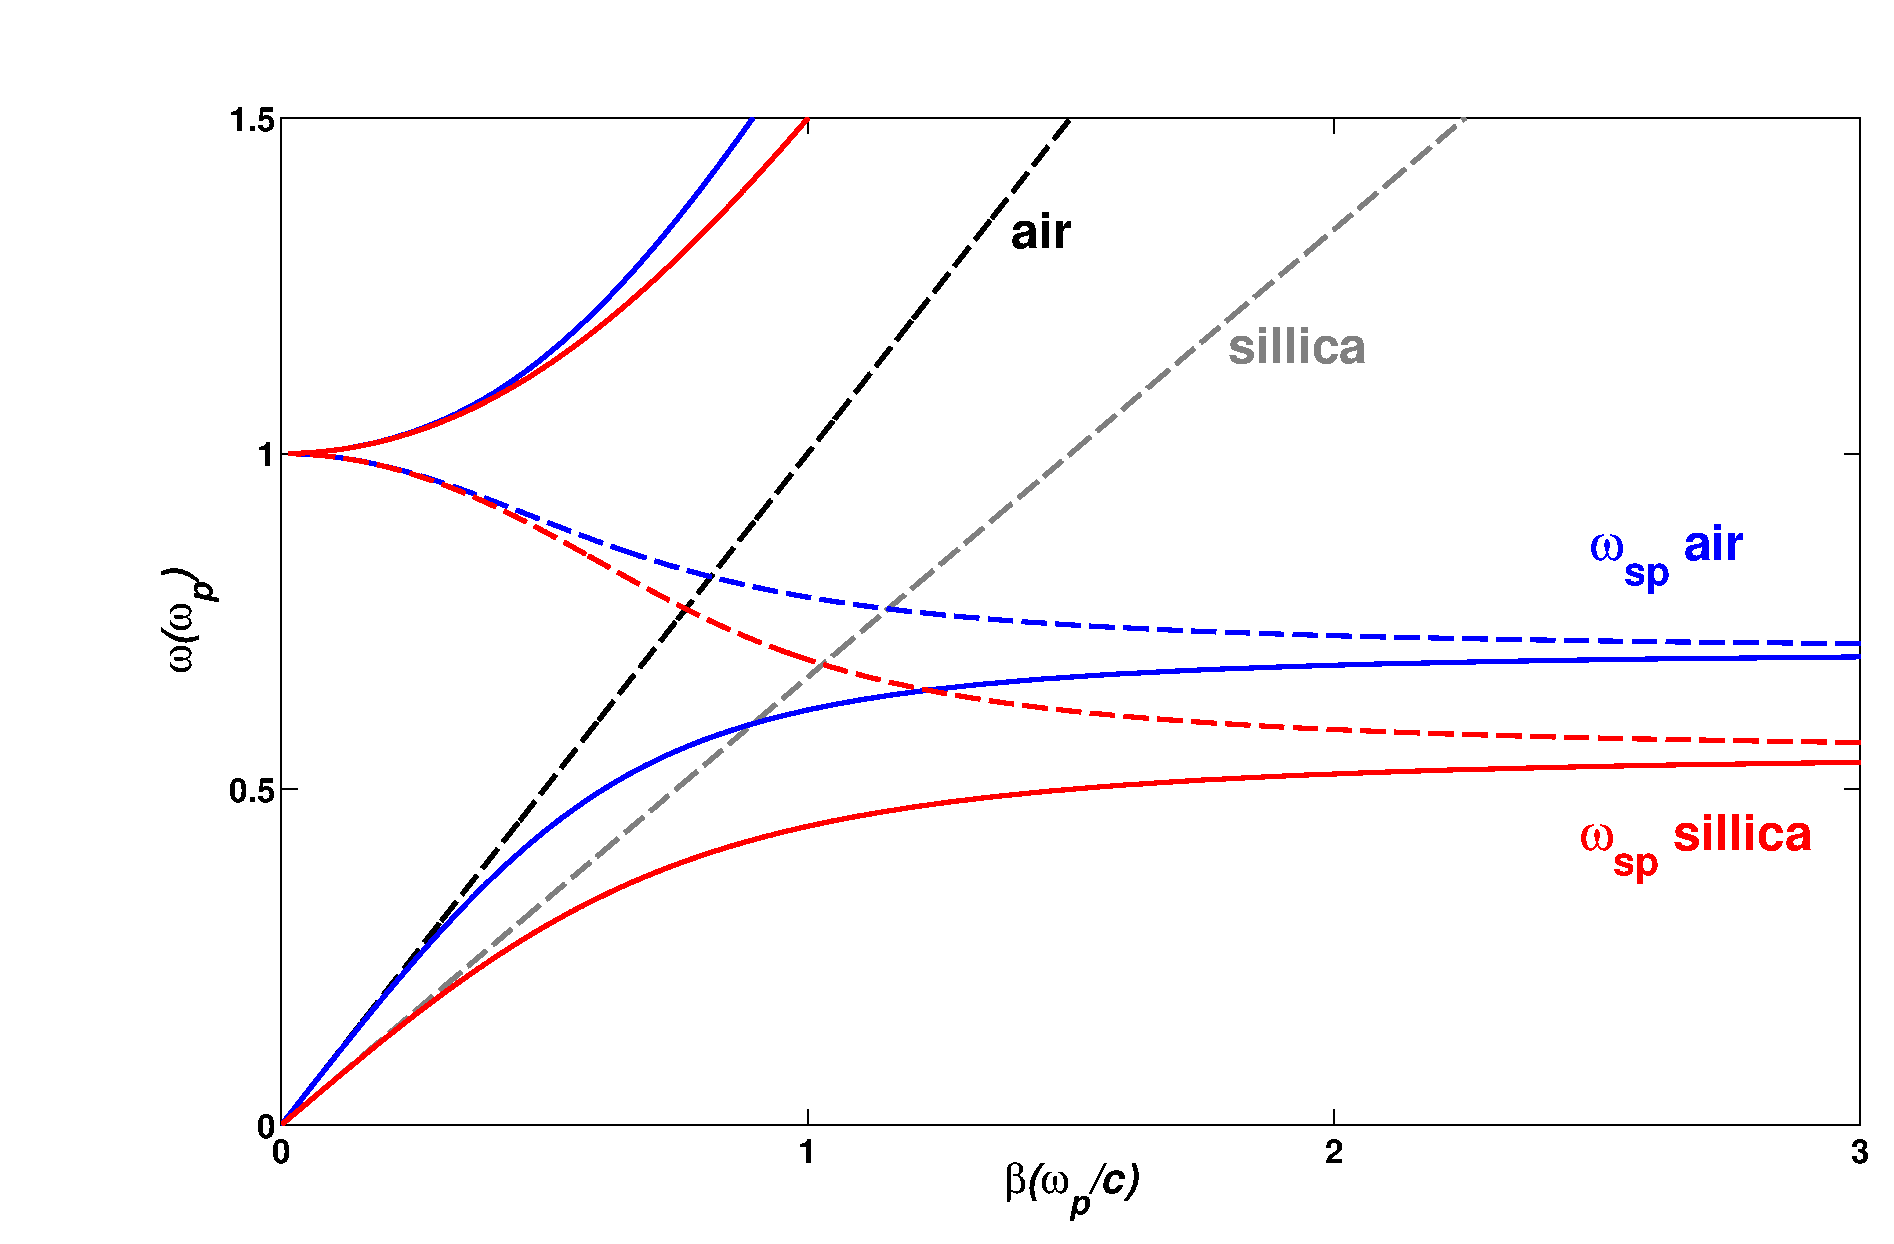
\includegraphics[scale=0.4]{THM/SPPdisp.eps}
\caption{\label{fig:SPPdisp}Dispersion relation of SPPs at the interface between a Drude metal with negligible collision frequency and air (blue curves) and silica (red curves).}
\end{figure}
For small wave vectors SPPs propagation constant $\beta$ is close to $k_0$ at the light line, in the opposite regime of the frequency close to surface plasmon frequency $\omega_p$. It also shows that the SPPs line lying to the right of the respective light lines of air and silica, so that SPPs are directed by light due to phase mismatching. The wave vector mismatch between SPPs and radiation modes needs to be overcome in order to excite or detect SPPs. This can be achieved by multiple methods~\cite{raether1988surface}. In the Otto configuration, light in a prism that is brought in close vicinity to a metal surface can excite SPPs through coupling to the evanescent field. Because light in the prism has a larger wave vector than that in air, it can be phase-matched to the SPPs. In the related Kretschmann-Raether geometry, coupling to SPPs occurs through a metal film that is deposited on a prism. In the grating coupling configuration, metal surface with a shallow grating of grooves or holes with lattice constant $a$. For the simple 1D grating of grooves depicted in Figure~\ref{fig:grating},
\begin{figure}[htb]
\centering
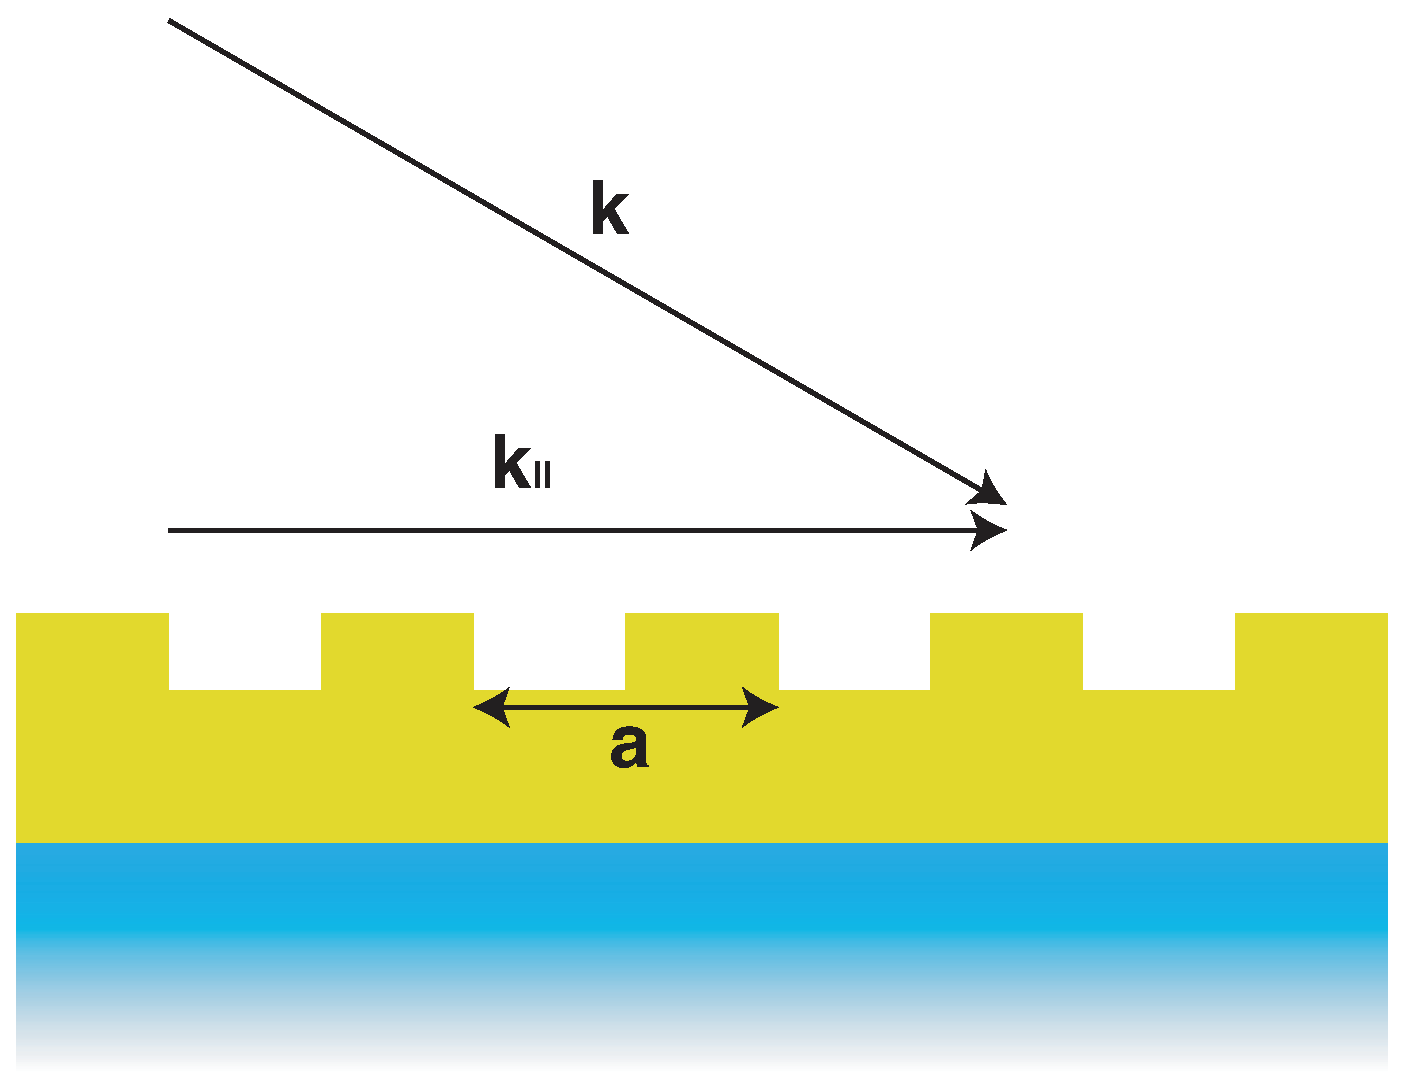
\includegraphics[scale=0.5]{THM/grating.eps}
\caption{\label{fig:grating}Phase-matching of light to SPPs the grating coupling configuration.}
\end{figure}
phase-matching takes place when the condition is fulfilled
\begin{equation}
\beta = k_0 \sin{\theta} \pm \nu g\text{,}
\end{equation}
where $g=\frac{2\pi}{a}$ is the reciprocal vector of the grating, and $\nu=(1,2,3\dots)$.
As with prism coupling, excitation of SPPs is detected as a minimum in the reflected light. The reverse process can also take place, SPPs propagating along a surface modulated with a grating can couple to light and thus radiate. 

%\bibliographystyle{unsrt}
%\bibliography{thesisbib}
\chapter{Experiment}
\label{c:exp}

\section{Atomic force microscopy}

\begin{figure}[htb]
\centering
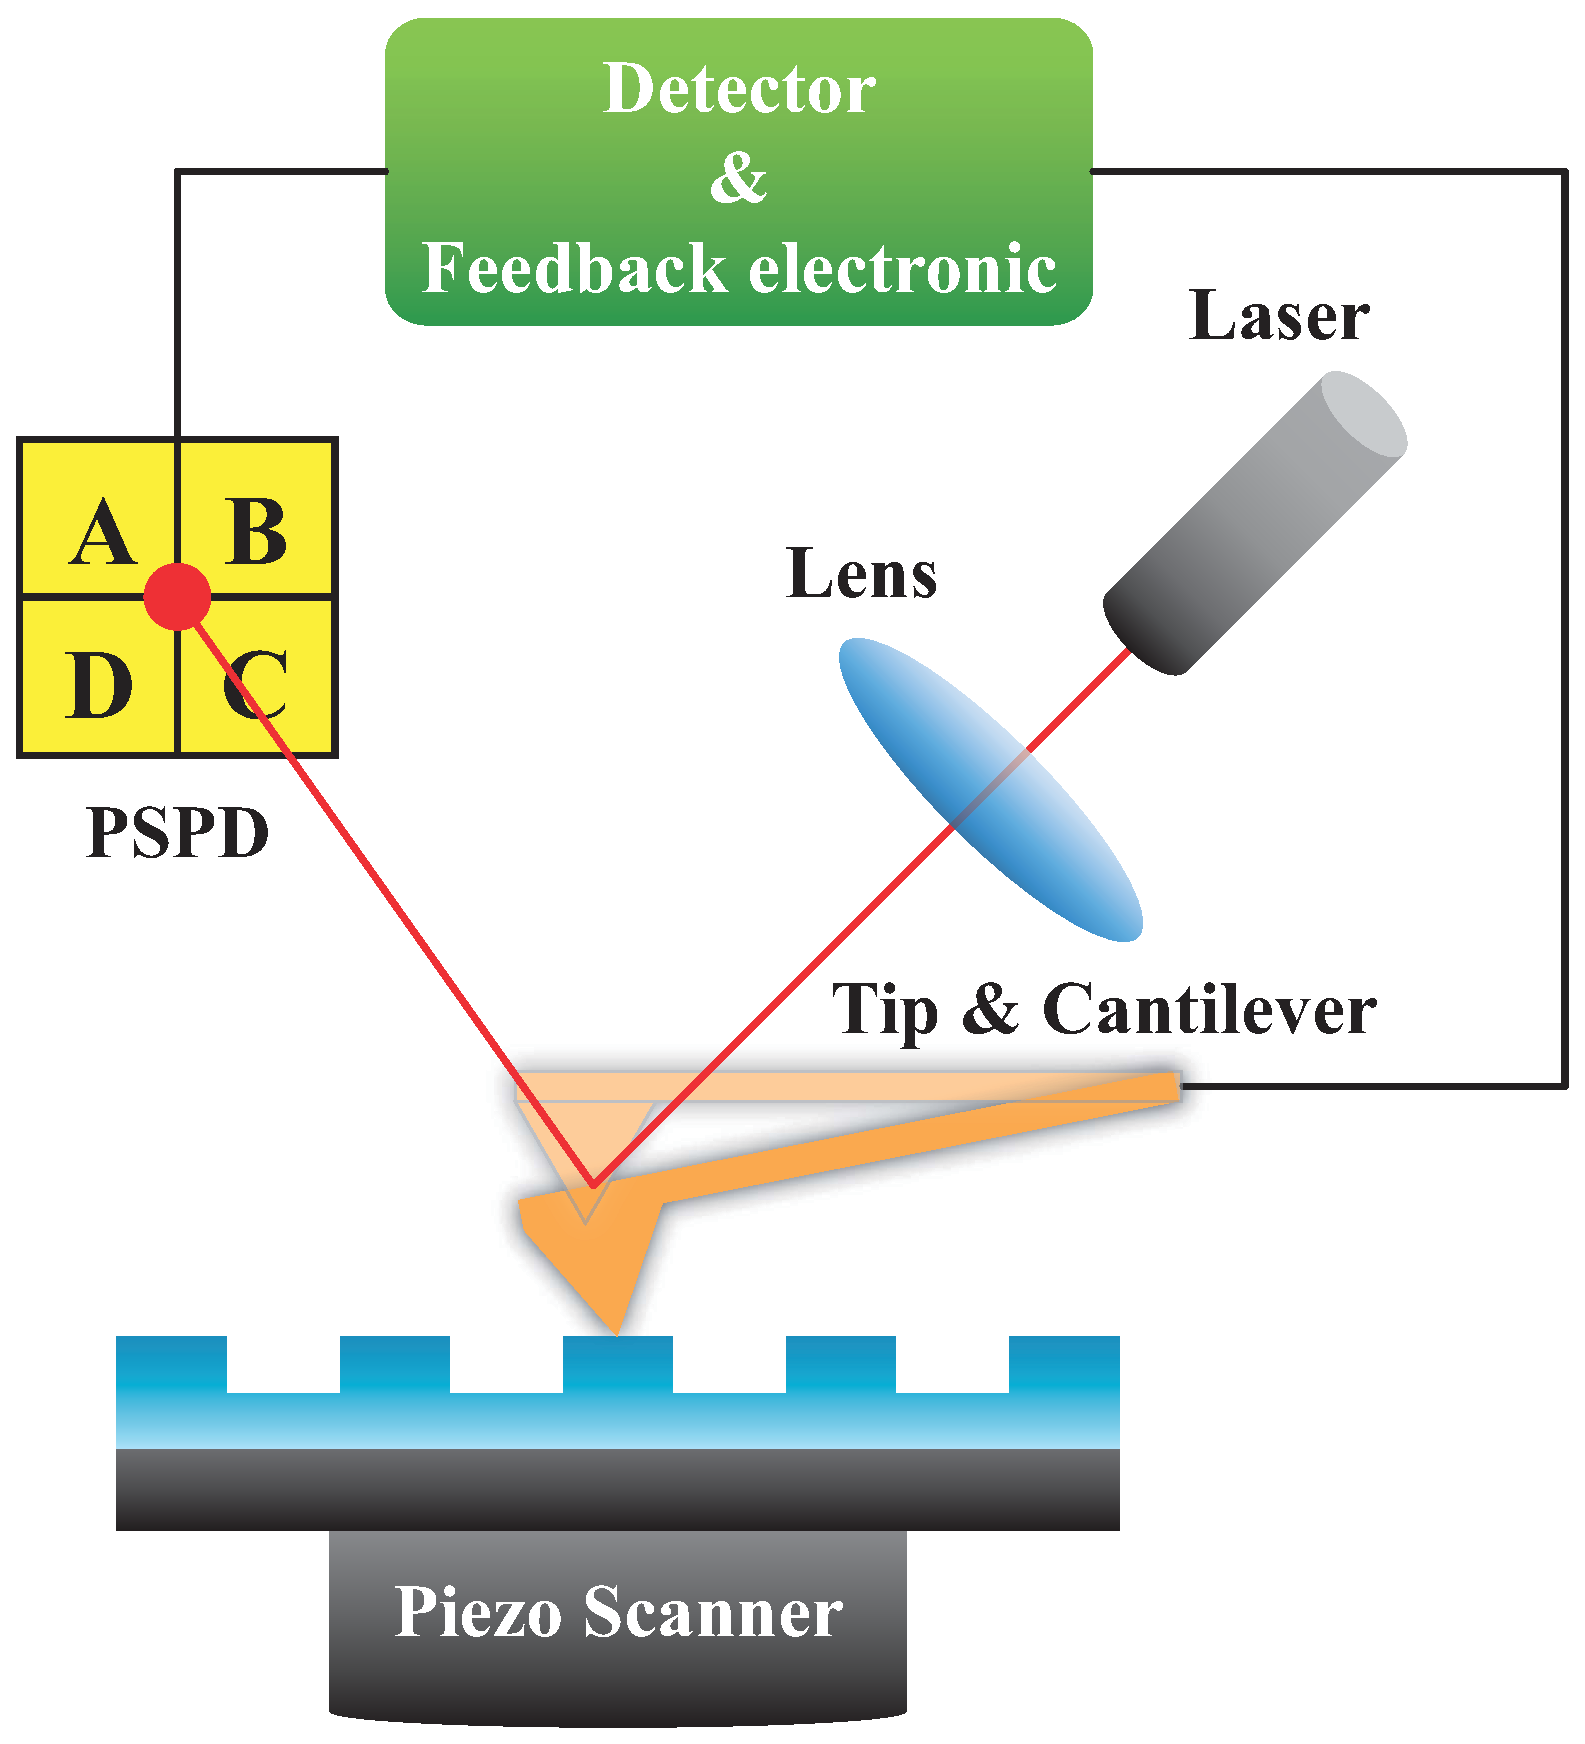
\includegraphics[scale=0.35]{EXP/afm1.eps}
\caption{\label{fig:afm1}Schematic of atomic force microscopy.}
\end{figure}
Atomic force microscope (AFM) is a type of scanning probe microscopes (SPM)~\cite{bennig1988atomic}.  The schematic of AFM is shown in Figure~\ref{fig:afm1}. AFM operates by measuring force between a probe and the specimen surfaces. In general,  the probe is a sharp tip at a cantilever's end. The cantilever can be deflected by atomic forces to sufficiently large amount, then AFM can measure the vertical and lateral deflections of the cantilever by using the optical system. A laser beam is transmitted to cantilever, and the reflected laser beam is detected with a position-sensitive photo detector (PSPD). PSPD is four-sectional that allows measuring not only vertical but lateral bending too(Figure~\ref{fig:afm2}). The output of the PSPD is provided to a computer for processing of the data for providing a topographical image of the surface with atomic resolution, and controlling the height between probe and specimen surfaces by applying voltage on piezoelectric scanner.
\begin{figure}[htb]
\centering
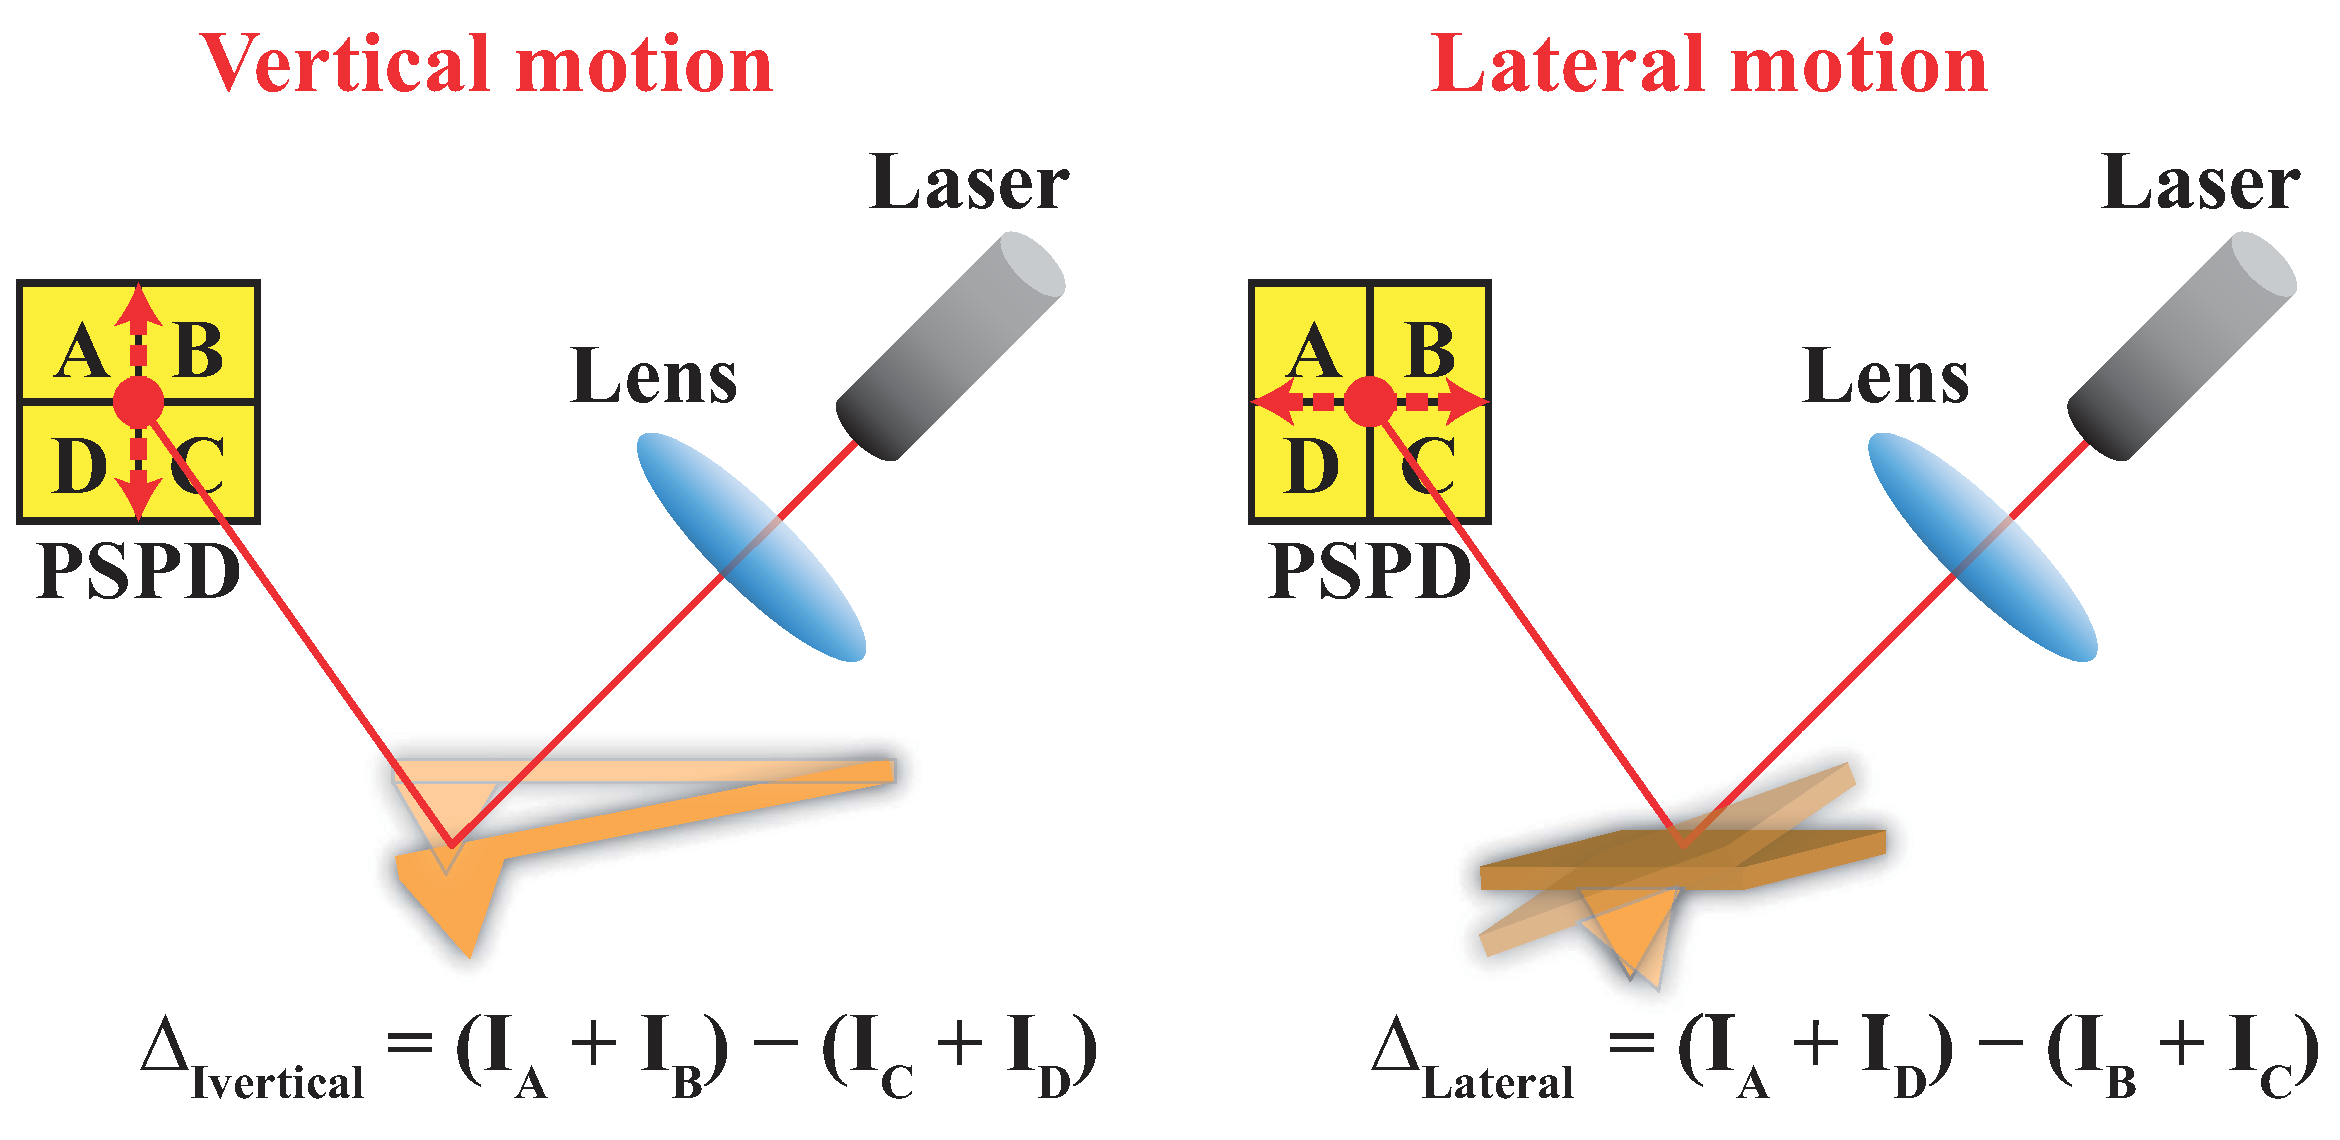
\includegraphics[scale=0.4]{EXP/afm2.eps}
\caption{\label{fig:afm2}Schematic of optical system for cantilever deflections detection.}
\end{figure}

The physical principle of the AFM operation is based on interaction between the probe tip and the specimen surface(Figure~\ref{fig:afm3}). When the cantilever approaches the specimen surface, Van der Waals forces start acting upon it . They are sufficiently far-ranging and are felt at the distance of a few tens of angstroms. Then at the distance of several angstroms repulsive force starts acting. In humid air a water layer is present on the specimen surface. The capillary force arises that holds the tip in contact with the surface and increases the minimum achievable interaction force. Electrostatic interaction between the probe and the sample may appear rather often. This can be both attraction and repulsion. Van der Waals attraction forces, capillary, electrostatic and repulsion forces at the point where the tip touches the sample and forces acting upon the tip from the deformed cantilever compensate each other in equilibrium. Based on the type and degree of this interaction the AFM modes can be broken down into contact and semi-contact(Figure~\ref{fig:afm3} ), which is a transition mode between the contact and non-contact modes.
\begin{figure}[htb]
\centering
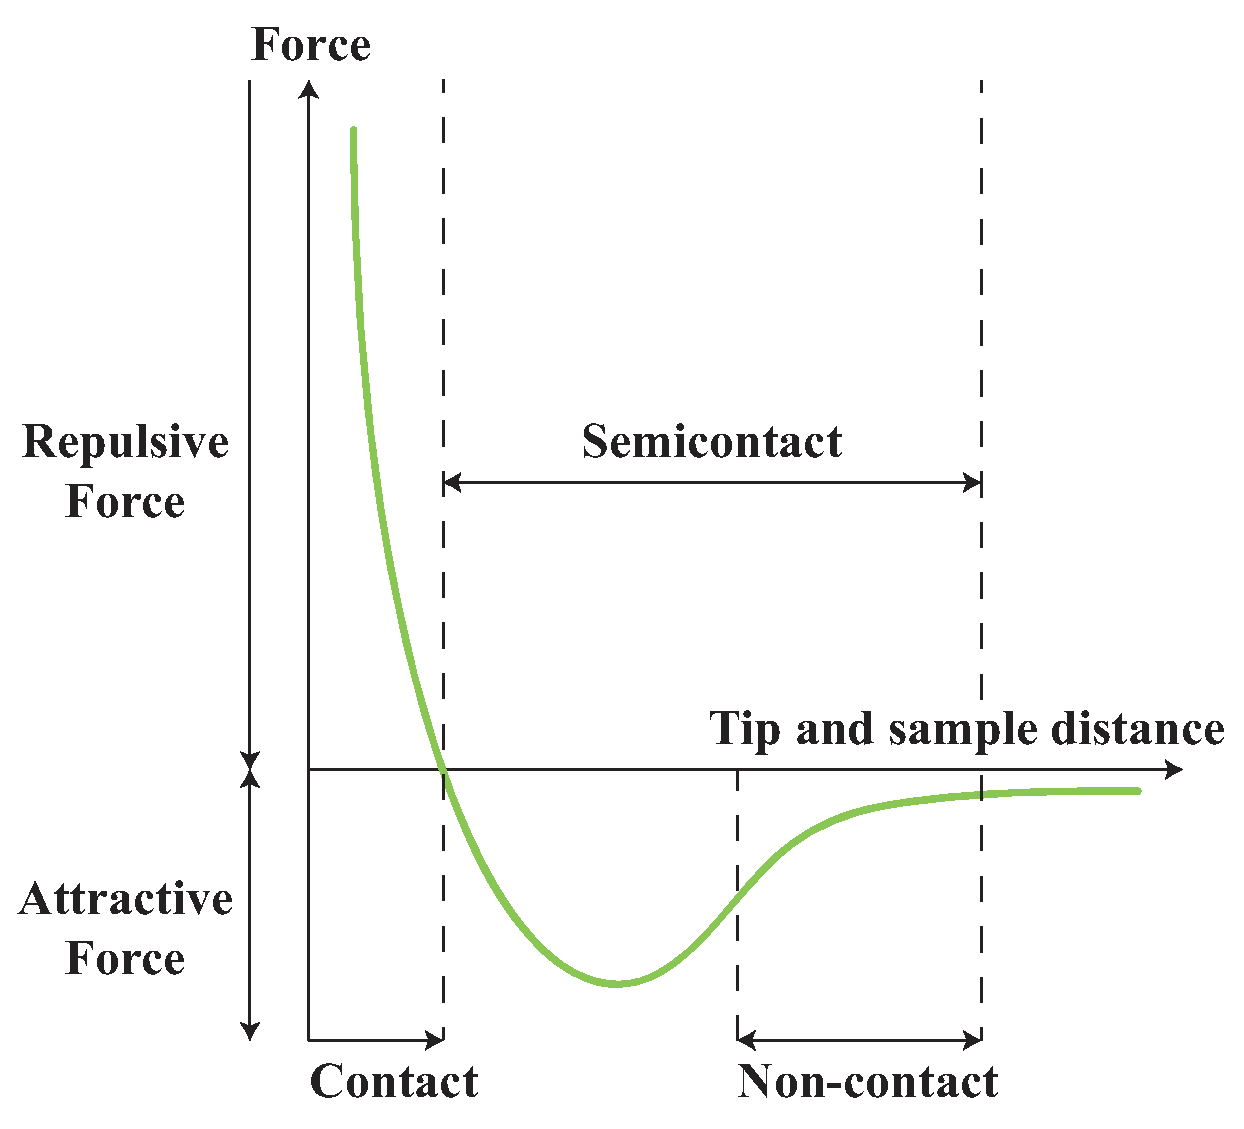
\includegraphics[scale=0.6]{EXP/afm3.eps}
\caption{\label{fig:afm3}Sketch of tip-sample forces.}
\end{figure}

\paragraph{Contact mode}

In contact mode of operation the cantilever deflection under scanning reflects repulsive force acting upon the tip. Repulsion force $\mathbf{F}$ acting upon the tip is related to the cantilever deflection value $\mathbf{x}$ under Hooke's law: $\mathbf{F}=-K \cdot  \mathbf{x}$, where $K$ is cantilever spring constant. The spring constant values for different cantilevers usually vary from 0.01 to several $\mathbf{N/m}$.

In our units the vertical cantilever deflection value is measured by means of the optical registration system and converted into electrical signal DFL (difference signal between the upper and lower halves of the PSPD) . In contact mode the DFL signal is used as a parameter characterizing the interaction force between the tip and the surface. There is a linear relationship between the DFL value and the force. In constant force mode of operation the deflection of the cantilever is maintained by the feedback circuitry on the preset value. So vertical displacement of the scanner under scanning reflects topography of sample under investigation.

Contact force microscopy is surface topography measurement in the contact mode.The microscope operation in the mode of maintaining constant interaction force between the tip and the surface sample, and is the base for measuring surface topography as well as for measuring local rigidity, local viscosity and local friction force. Constant force mode has some advantages and disadvantages. Main advantage of constant force mode is possible to measure with high resolution simultaneously with topography and some other characteristics, such as friction forces, spreading resistance etc. Constant force mode has also some disadvantages. Speed of scanning is restricted by the response time of feedback system. When exploring soft samples they can be destroyed by the scratching because the probe scanning tip is in direct contact with the surface. Therefore, under scanning soft unhomogeneous samples the local flexure of sample surface varies. As a result acquired topography of the sample can be proved distorted. Possible existence of substantial capillary forces imposed by a liquid adsorption layer can decrease the resolution.

\paragraph{Semi-contact mode}

The semi-contac mode can be characterized by some advantages in comparison with contact mode. First of all, in this mode the force of pressure of the cantilever onto the surface is less, that allows to work with softer materials such as polymers and bio-organics. The semi contact mode is also more sensitive to the interaction with the surface that gives a possibility to investigate some characteristics of the surface distribution of magnetic and electric domains, elasticity and viscosity of the surface. 

Widely used semi-contact mode has some disadvantage concerned with the usage of the feedback circuit. The scanning speed in semi-contact mode is restricted by the feedback circuit reaction time. This disadvantage can be overcome by the fact that under scanning new value of cantilever oscillation amplitude (and error signal) usually is achieved faster than preset value of the cantilever oscillation amplitude can be reached by the feedback system. Time of the reaching new value of the oscillation amplitude is determined by the oscillation period and Q-quality of the cantilever.
The feedback error signal, emerging when scanning in the semi-contact mode, contains some additional information about the topography. It can be utilized for achieving a more precise recovery of the relief. 

Additionally, similarly to the contact error mode, which can be considered as intermediate between the constant force mode and constant height mode, the feedback gain factor (i.e. the feedback processing speed) can be adjusted for the system to be able to trace subtle changes of the relief and to be too slow to trace the steep changes. Then, when the probe travels over minor irregularities, scanning will be carried out with an almost constant piezo scanner length. As a result, the slow changes of the relief will hardly show up on the images, and the steep changes will appear in high contrast. This may be helpful in finding minor irregularities on large areas against major sloping relief features. It must be noted that height of the minor irregularities must be less than amplitude of cantilever oscillation.

\section{Scanning electron microscopy}

The scanning electron microscope (SEM) is used for the observation of specimen surfaces~\cite{von1938elektronen}. When the specimen is irradiated with a fine electron beam, secondary electrons are emitted from the specimen surface. Topography of the surface can be observed by two-dimensional scanning of the electron probe over the surface and acquisition of an image from the detected secondary electrons. The concept schematic of commercial SEM (JEOL, JSM-6500F) is shown in Figure~\ref{fig:sem1}. The basic unit is composed of an electron optical system, a specimen stage, a secondary-electron detector, an image display unit, and an operation system. The electron optical system consists of an electron gun, a condenser lens and an objective lens to produce an electron probe, a scanning coil to scan the electron probe, and other components. The system inside of the microscope column are kept at vacuum.
\begin{figure}[htb]
\centering
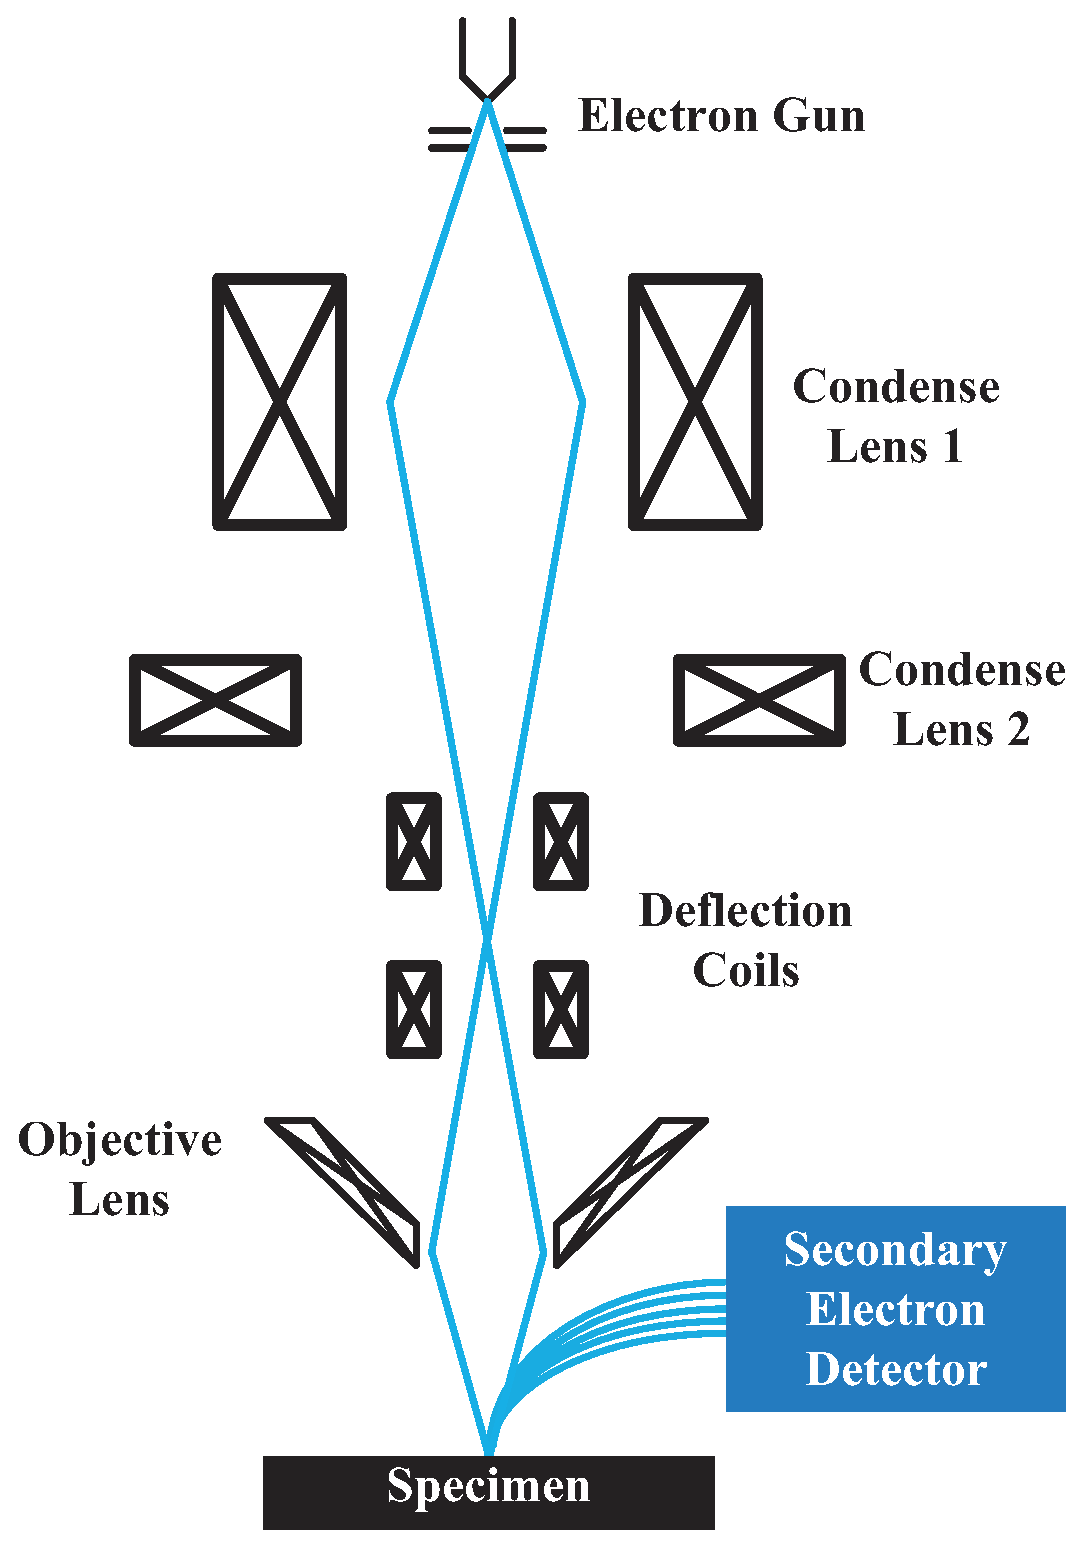
\includegraphics[scale=0.5]{EXP/SEM.eps}
\caption{\label{fig:sem1}Basic construction of a scanning electron microscopy.}
\end{figure}


The JSM-6500F utilizes a Schottky type field-emission (T-FE) gun for the electron source. The T-FE gun can constantly supply the surface of the cathode with zirconium oxide by heating the surface of cathode to 1800 K. For this reason, it can easily obtain stable and high probe current (range from several pA to 100 nA) compared with the traditional thermal emission electron gun and cold field-emission gun.

The magnetic condenser and objective lens system act to control the diameter of the beam as well as to focus the beam on the specimen due to a rotationally-symmetric magnetic field is formed when we pass a direct electric current through a coilwound electric wire in the magnetic lens. A pair of deflector coils, which between the condenser and objective lens, controlled by the scan generator, which are responsible for rastering that focused beam across the specimen surface. The size of the rastering pattern is under magnification control. The beam is rastered from left to right and top to bottom. There is a one-to-one correspondence between the rastering pattern on the specimen and the rastering pattern used to produce the image on the monitor. The resolution we choose to image at will obviously affect the number of pixels per row as well as the number of rows that constitute the scanned area.

The signal is generated from the specimen, and collected by the detector and subsequently processed to generate the image. That processing takes the intensity of the signal coming from a pixel on the specimen and converts it to a grayscale value of the corresponding monitor pixel. The monitor image is a two dimensional rastered pattern of grayscale values.

With the beam focused on the specimen surface, all we need to do to change magnification is to change the size of the rastered area on the specimen. The size of the monitor raster pattern is constant. Magnification will increase if we reduce the size of the area scanned on the specimen.

%\bibliographystyle{unsrt}
%\bibliography{thesisbib}           =>  \chapter{Experiment}
\label{c:exp}

\section{Atomic force microscopy}

\begin{figure}[htb]
\centering
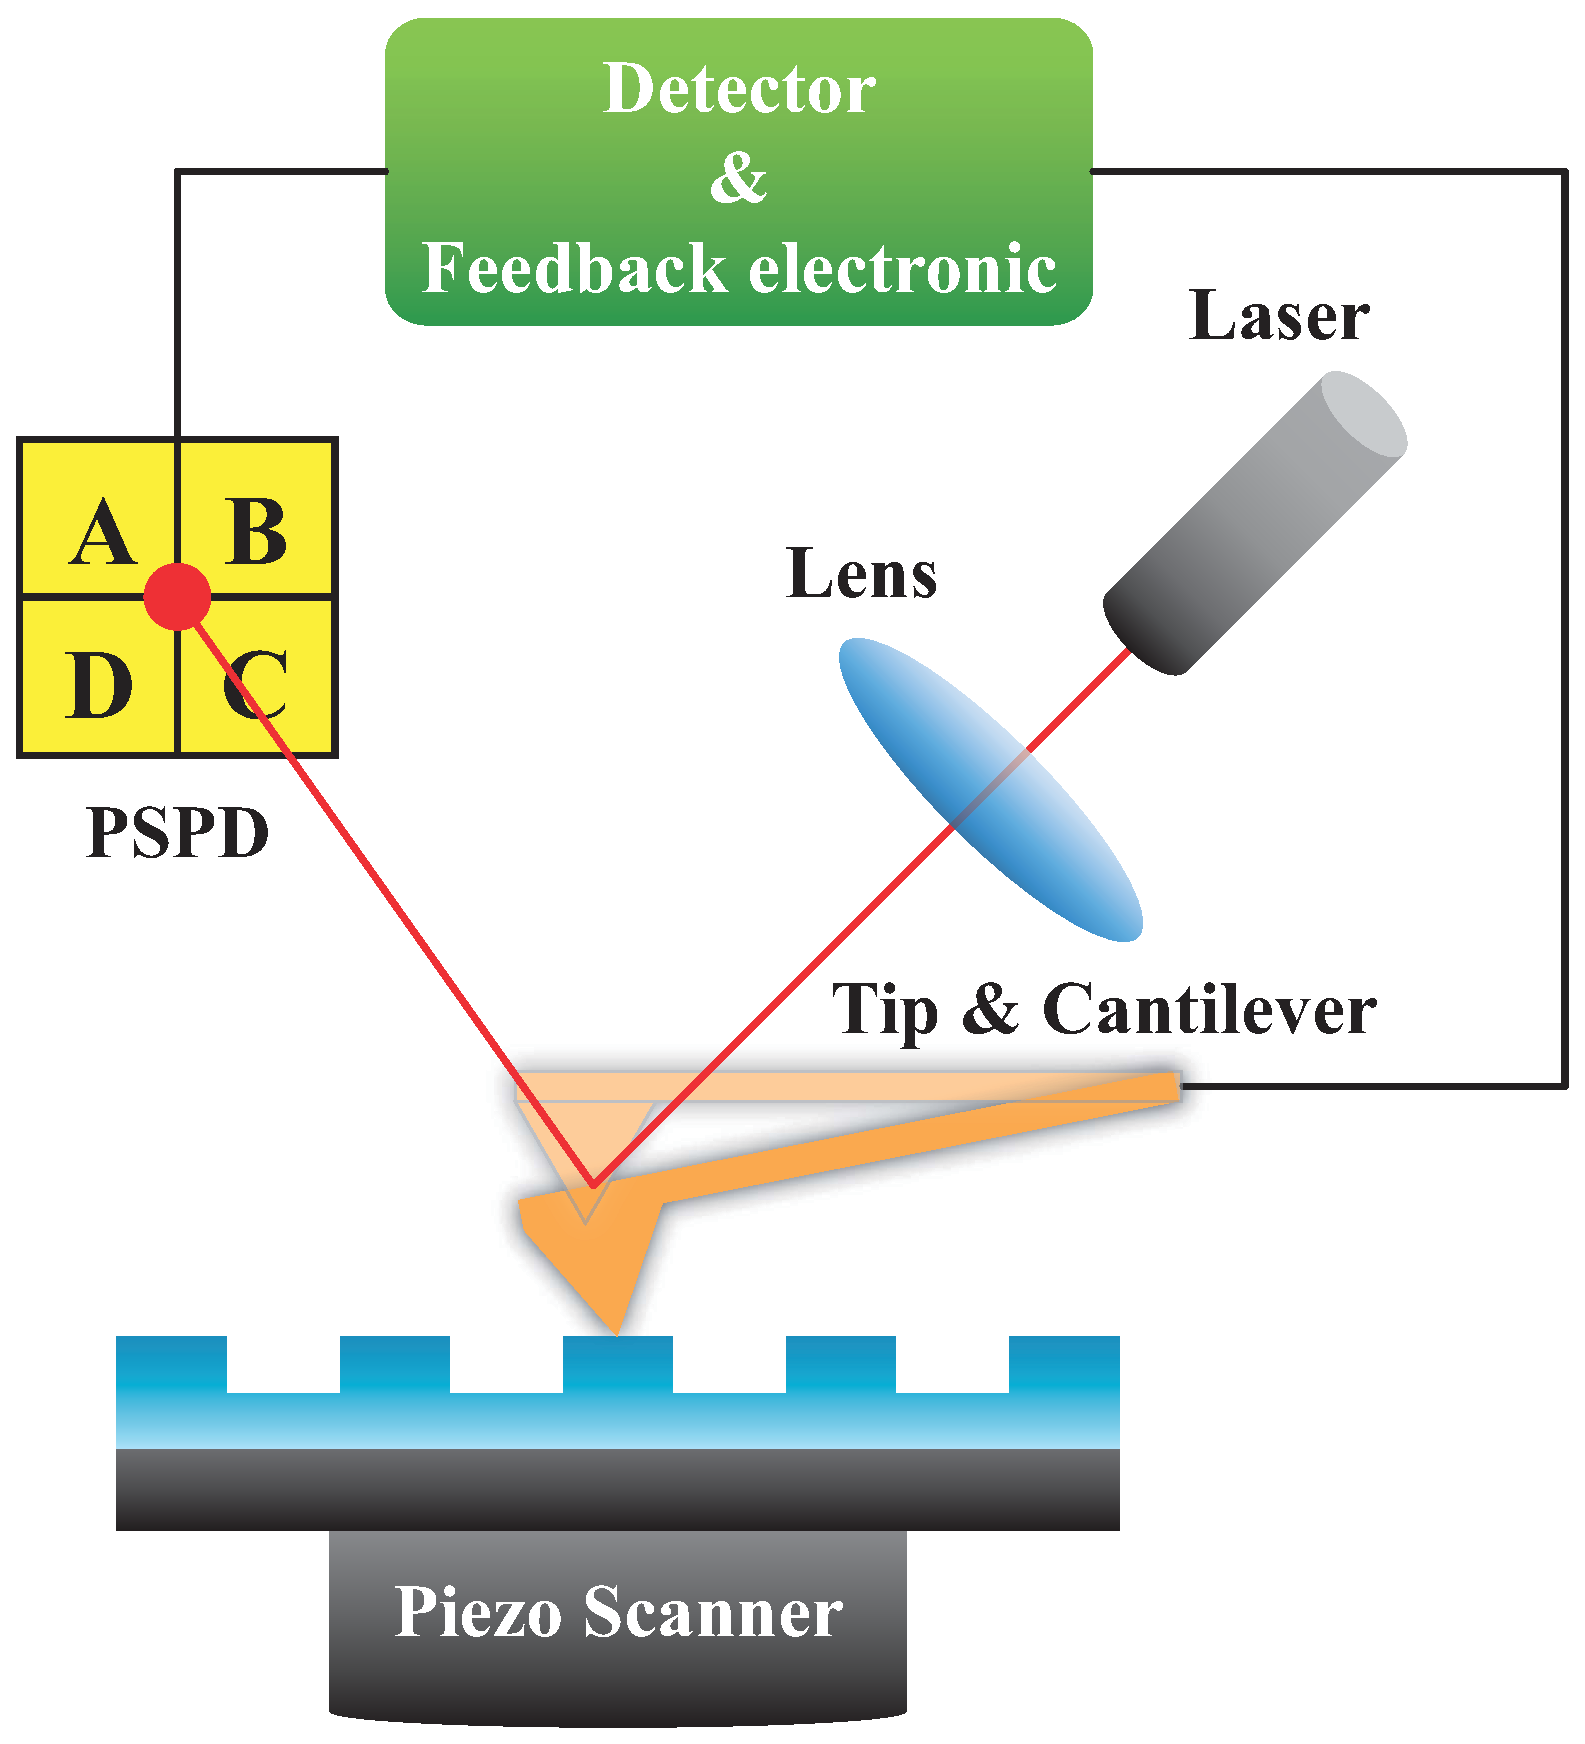
\includegraphics[scale=0.35]{EXP/afm1.eps}
\caption{\label{fig:afm1}Schematic of atomic force microscopy.}
\end{figure}
Atomic force microscope (AFM) is a type of scanning probe microscopes (SPM)~\cite{bennig1988atomic}.  The schematic of AFM is shown in Figure~\ref{fig:afm1}. AFM operates by measuring force between a probe and the specimen surfaces. In general,  the probe is a sharp tip at a cantilever's end. The cantilever can be deflected by atomic forces to sufficiently large amount, then AFM can measure the vertical and lateral deflections of the cantilever by using the optical system. A laser beam is transmitted to cantilever, and the reflected laser beam is detected with a position-sensitive photo detector (PSPD). PSPD is four-sectional that allows measuring not only vertical but lateral bending too(Figure~\ref{fig:afm2}). The output of the PSPD is provided to a computer for processing of the data for providing a topographical image of the surface with atomic resolution, and controlling the height between probe and specimen surfaces by applying voltage on piezoelectric scanner.
\begin{figure}[htb]
\centering
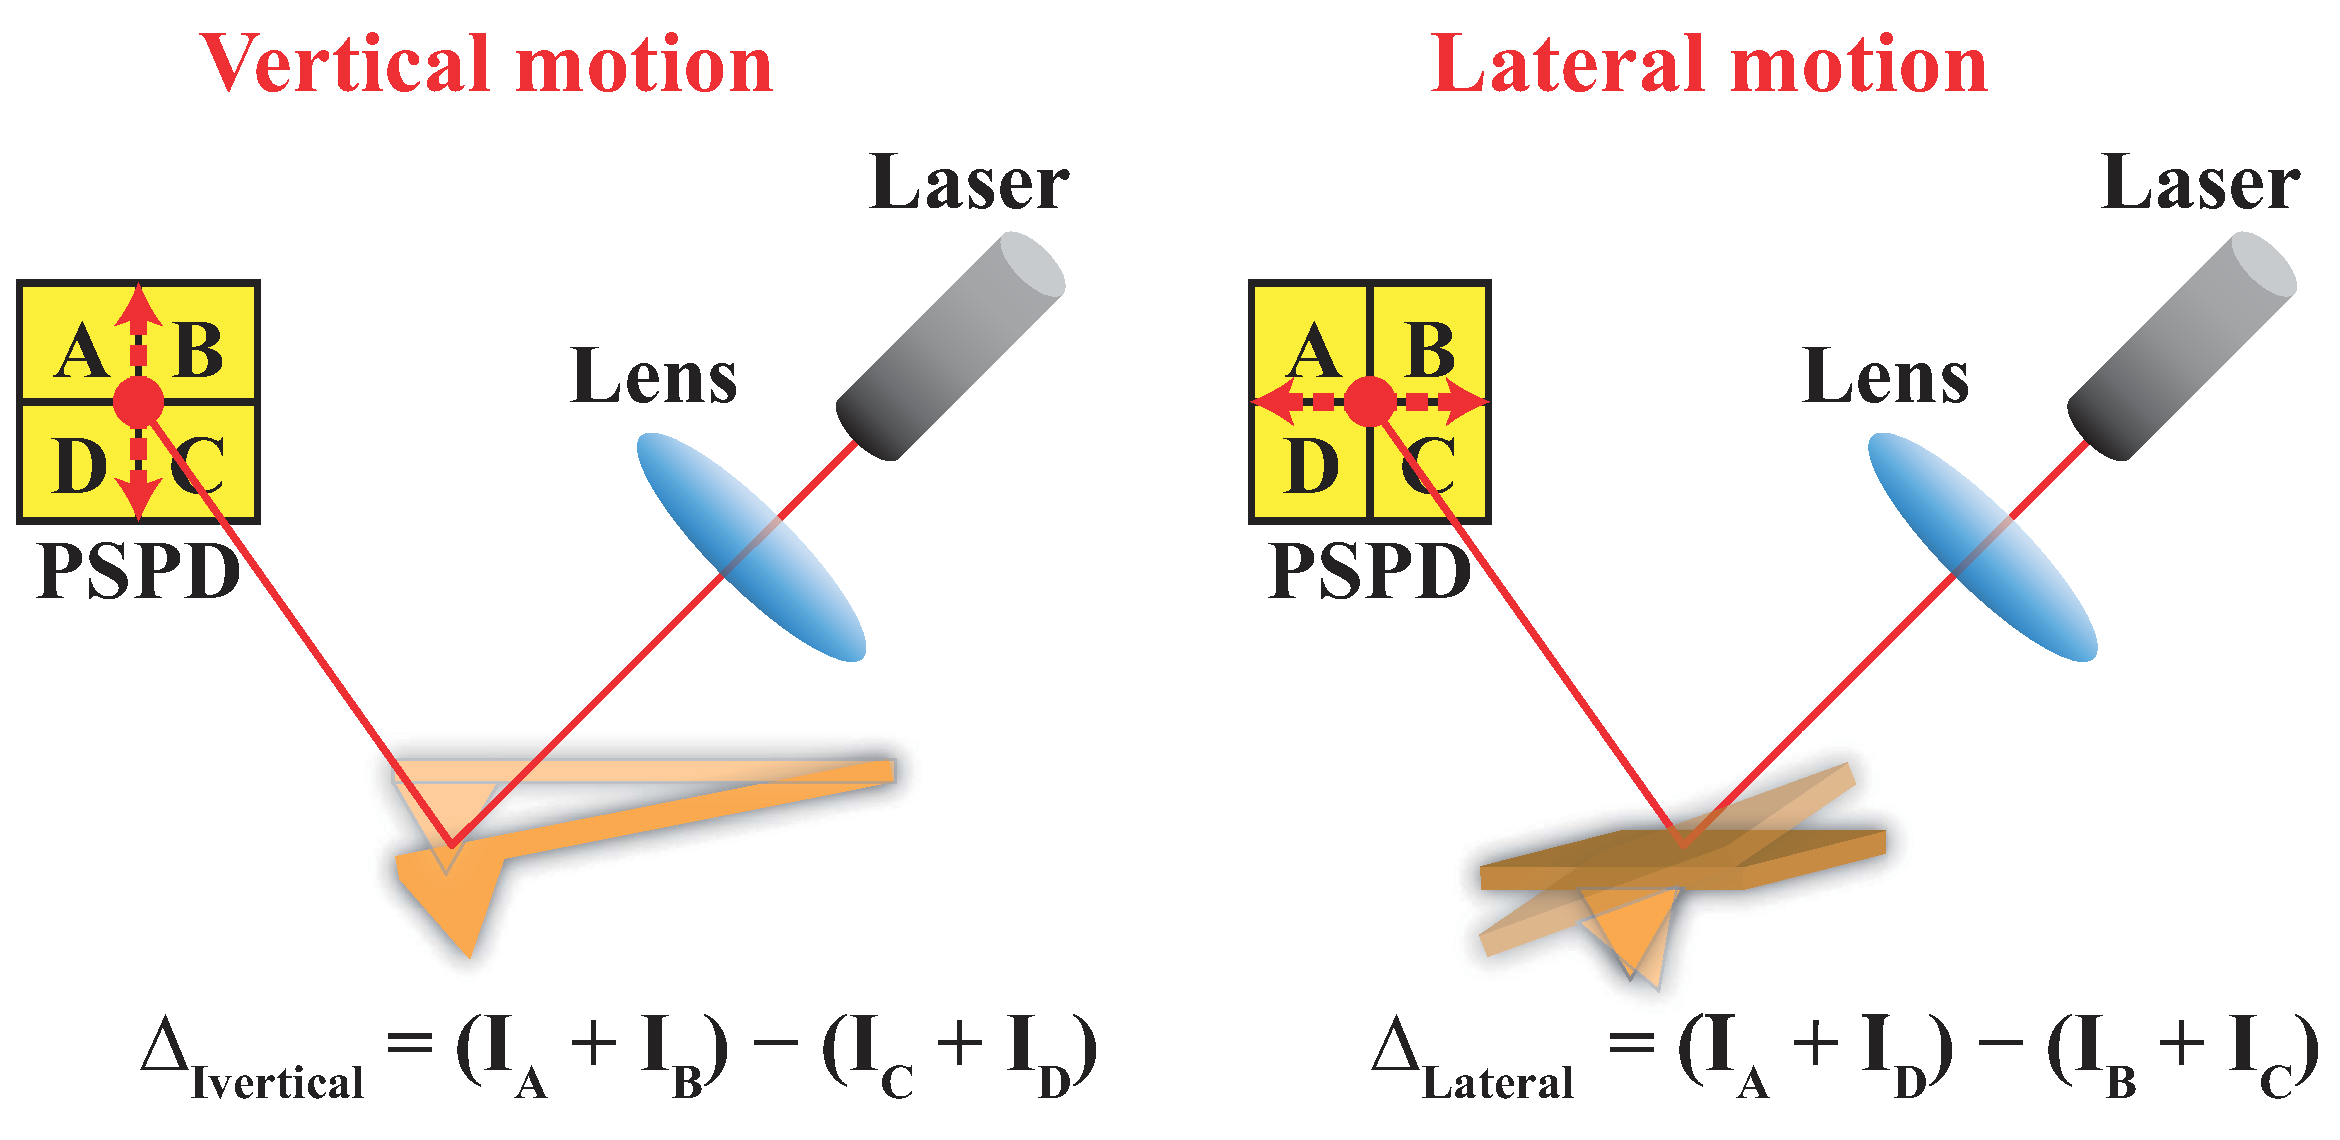
\includegraphics[scale=0.4]{EXP/afm2.eps}
\caption{\label{fig:afm2}Schematic of optical system for cantilever deflections detection.}
\end{figure}

The physical principle of the AFM operation is based on interaction between the probe tip and the specimen surface(Figure~\ref{fig:afm3}). When the cantilever approaches the specimen surface, Van der Waals forces start acting upon it . They are sufficiently far-ranging and are felt at the distance of a few tens of angstroms. Then at the distance of several angstroms repulsive force starts acting. In humid air a water layer is present on the specimen surface. The capillary force arises that holds the tip in contact with the surface and increases the minimum achievable interaction force. Electrostatic interaction between the probe and the sample may appear rather often. This can be both attraction and repulsion. Van der Waals attraction forces, capillary, electrostatic and repulsion forces at the point where the tip touches the sample and forces acting upon the tip from the deformed cantilever compensate each other in equilibrium. Based on the type and degree of this interaction the AFM modes can be broken down into contact and semi-contact(Figure~\ref{fig:afm3} ), which is a transition mode between the contact and non-contact modes.
\begin{figure}[htb]
\centering
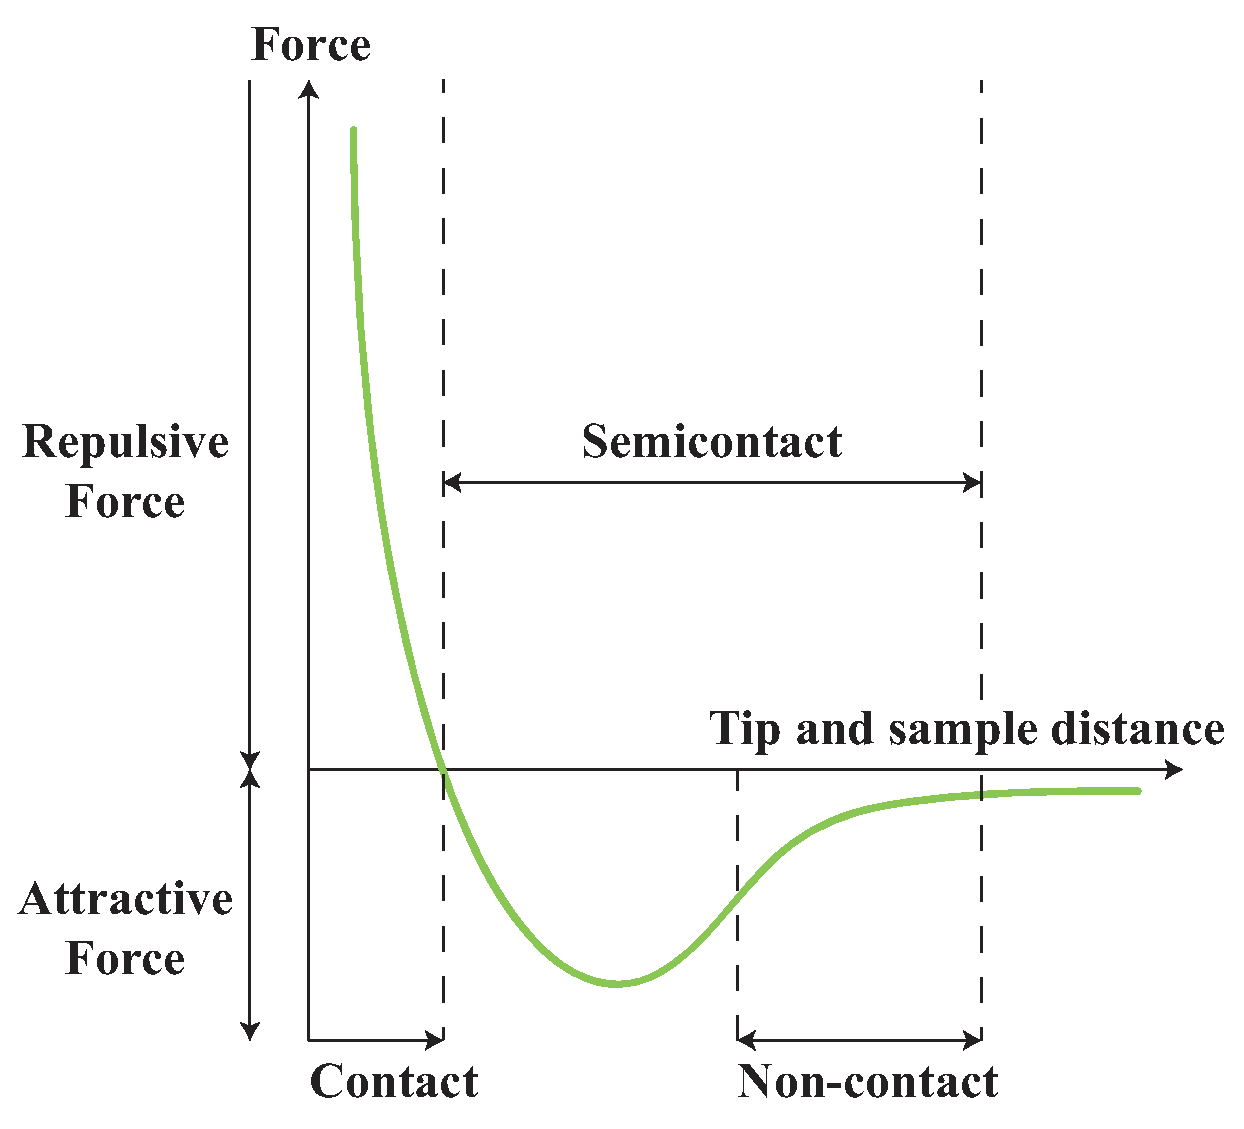
\includegraphics[scale=0.6]{EXP/afm3.eps}
\caption{\label{fig:afm3}Sketch of tip-sample forces.}
\end{figure}

\paragraph{Contact mode}

In contact mode of operation the cantilever deflection under scanning reflects repulsive force acting upon the tip. Repulsion force $\mathbf{F}$ acting upon the tip is related to the cantilever deflection value $\mathbf{x}$ under Hooke's law: $\mathbf{F}=-K \cdot  \mathbf{x}$, where $K$ is cantilever spring constant. The spring constant values for different cantilevers usually vary from 0.01 to several $\mathbf{N/m}$.

In our units the vertical cantilever deflection value is measured by means of the optical registration system and converted into electrical signal DFL (difference signal between the upper and lower halves of the PSPD) . In contact mode the DFL signal is used as a parameter characterizing the interaction force between the tip and the surface. There is a linear relationship between the DFL value and the force. In constant force mode of operation the deflection of the cantilever is maintained by the feedback circuitry on the preset value. So vertical displacement of the scanner under scanning reflects topography of sample under investigation.

Contact force microscopy is surface topography measurement in the contact mode.The microscope operation in the mode of maintaining constant interaction force between the tip and the surface sample, and is the base for measuring surface topography as well as for measuring local rigidity, local viscosity and local friction force. Constant force mode has some advantages and disadvantages. Main advantage of constant force mode is possible to measure with high resolution simultaneously with topography and some other characteristics, such as friction forces, spreading resistance etc. Constant force mode has also some disadvantages. Speed of scanning is restricted by the response time of feedback system. When exploring soft samples they can be destroyed by the scratching because the probe scanning tip is in direct contact with the surface. Therefore, under scanning soft unhomogeneous samples the local flexure of sample surface varies. As a result acquired topography of the sample can be proved distorted. Possible existence of substantial capillary forces imposed by a liquid adsorption layer can decrease the resolution.

\paragraph{Semi-contact mode}

The semi-contac mode can be characterized by some advantages in comparison with contact mode. First of all, in this mode the force of pressure of the cantilever onto the surface is less, that allows to work with softer materials such as polymers and bio-organics. The semi contact mode is also more sensitive to the interaction with the surface that gives a possibility to investigate some characteristics of the surface distribution of magnetic and electric domains, elasticity and viscosity of the surface. 

Widely used semi-contact mode has some disadvantage concerned with the usage of the feedback circuit. The scanning speed in semi-contact mode is restricted by the feedback circuit reaction time. This disadvantage can be overcome by the fact that under scanning new value of cantilever oscillation amplitude (and error signal) usually is achieved faster than preset value of the cantilever oscillation amplitude can be reached by the feedback system. Time of the reaching new value of the oscillation amplitude is determined by the oscillation period and Q-quality of the cantilever.
The feedback error signal, emerging when scanning in the semi-contact mode, contains some additional information about the topography. It can be utilized for achieving a more precise recovery of the relief. 

Additionally, similarly to the contact error mode, which can be considered as intermediate between the constant force mode and constant height mode, the feedback gain factor (i.e. the feedback processing speed) can be adjusted for the system to be able to trace subtle changes of the relief and to be too slow to trace the steep changes. Then, when the probe travels over minor irregularities, scanning will be carried out with an almost constant piezo scanner length. As a result, the slow changes of the relief will hardly show up on the images, and the steep changes will appear in high contrast. This may be helpful in finding minor irregularities on large areas against major sloping relief features. It must be noted that height of the minor irregularities must be less than amplitude of cantilever oscillation.

\section{Scanning electron microscopy}

The scanning electron microscope (SEM) is used for the observation of specimen surfaces~\cite{von1938elektronen}. When the specimen is irradiated with a fine electron beam, secondary electrons are emitted from the specimen surface. Topography of the surface can be observed by two-dimensional scanning of the electron probe over the surface and acquisition of an image from the detected secondary electrons. The concept schematic of commercial SEM (JEOL, JSM-6500F) is shown in Figure~\ref{fig:sem1}. The basic unit is composed of an electron optical system, a specimen stage, a secondary-electron detector, an image display unit, and an operation system. The electron optical system consists of an electron gun, a condenser lens and an objective lens to produce an electron probe, a scanning coil to scan the electron probe, and other components. The system inside of the microscope column are kept at vacuum.
\begin{figure}[htb]
\centering
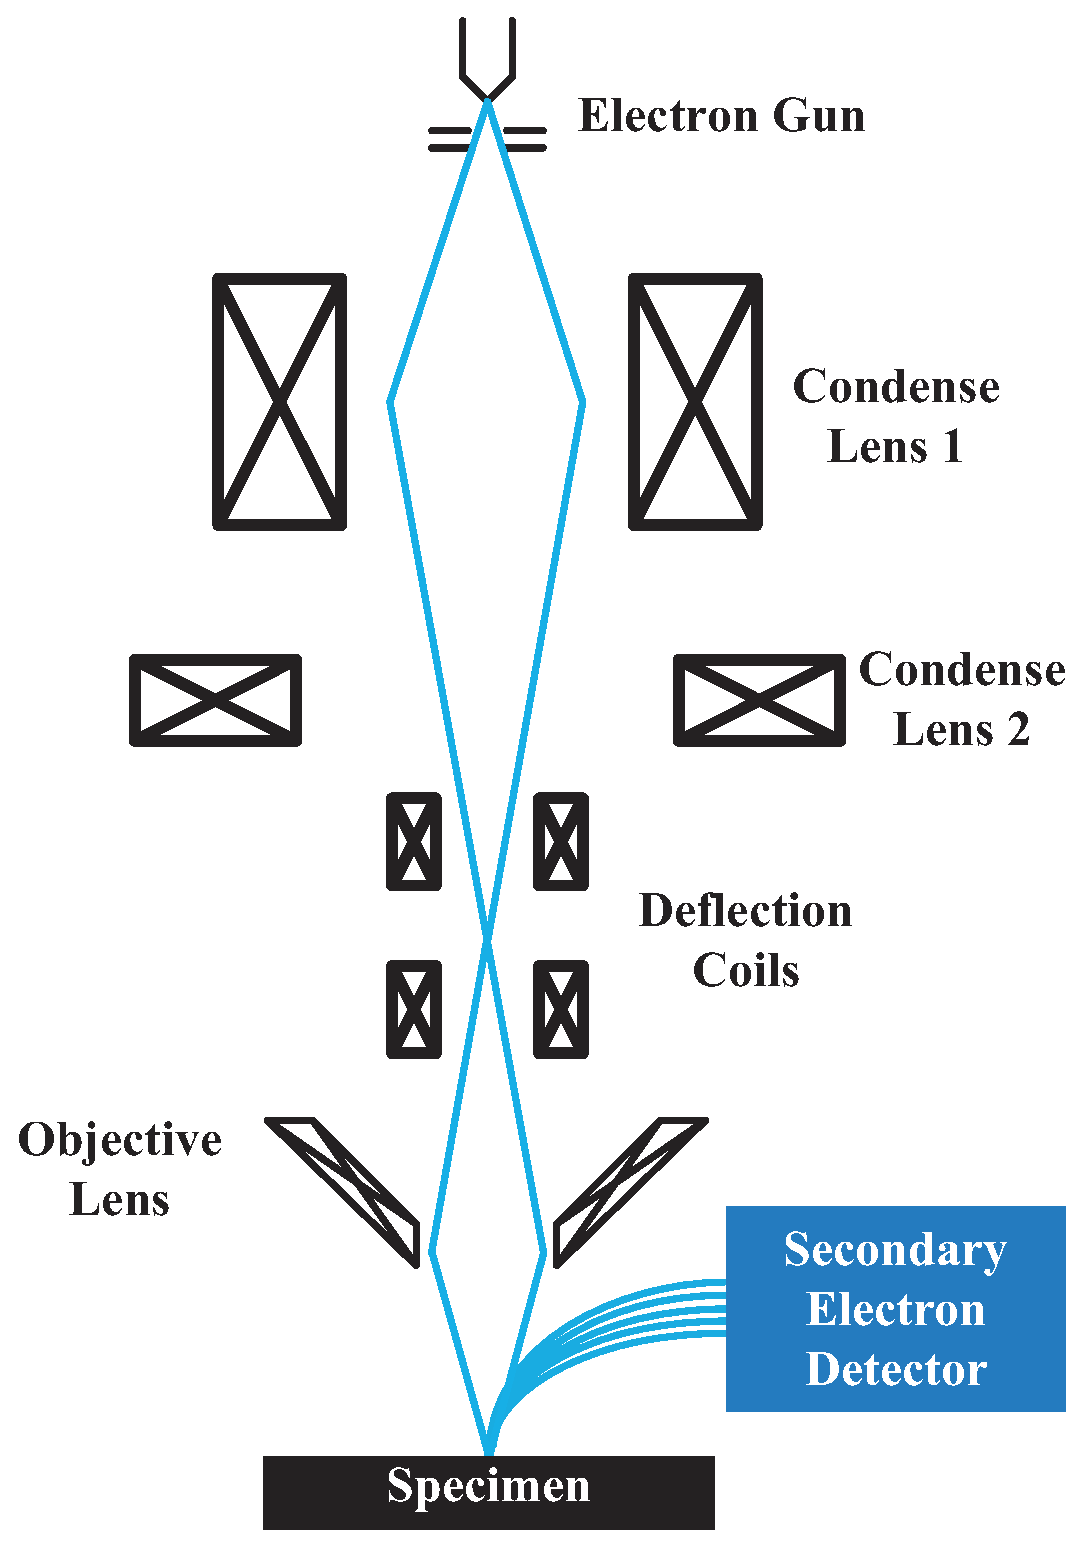
\includegraphics[scale=0.5]{EXP/SEM.eps}
\caption{\label{fig:sem1}Basic construction of a scanning electron microscopy.}
\end{figure}


The JSM-6500F utilizes a Schottky type field-emission (T-FE) gun for the electron source. The T-FE gun can constantly supply the surface of the cathode with zirconium oxide by heating the surface of cathode to 1800 K. For this reason, it can easily obtain stable and high probe current (range from several pA to 100 nA) compared with the traditional thermal emission electron gun and cold field-emission gun.

The magnetic condenser and objective lens system act to control the diameter of the beam as well as to focus the beam on the specimen due to a rotationally-symmetric magnetic field is formed when we pass a direct electric current through a coilwound electric wire in the magnetic lens. A pair of deflector coils, which between the condenser and objective lens, controlled by the scan generator, which are responsible for rastering that focused beam across the specimen surface. The size of the rastering pattern is under magnification control. The beam is rastered from left to right and top to bottom. There is a one-to-one correspondence between the rastering pattern on the specimen and the rastering pattern used to produce the image on the monitor. The resolution we choose to image at will obviously affect the number of pixels per row as well as the number of rows that constitute the scanned area.

The signal is generated from the specimen, and collected by the detector and subsequently processed to generate the image. That processing takes the intensity of the signal coming from a pixel on the specimen and converts it to a grayscale value of the corresponding monitor pixel. The monitor image is a two dimensional rastered pattern of grayscale values.

With the beam focused on the specimen surface, all we need to do to change magnification is to change the size of the rastered area on the specimen. The size of the monitor raster pattern is constant. Magnification will increase if we reduce the size of the area scanned on the specimen.

%\bibliographystyle{unsrt}
%\bibliography{thesisbib}
     \end{verbatim}
    最後記得在每個有附參考文獻的章節加上產生參考文獻的指令,即在\href{run:./introduction.tex}{introduction.tex}、\href{run:./THM.tex}{THM.tex}和\href{run:./EXP.tex}{EXP.tex}三個檔案裡最後啟動下面兩行指令
     \begin{verbatim}
%\bibliographystyle{unsrt} => \bibliographystyle{unsrt}
%\bibliography{thesisbib}  =>  \bibliography{thesisbib}
     \end{verbatim}
    而編譯時則需要對有附參考文獻的\href{run:./introduction.tex}{introduction.tex}、\href{run:./THM.tex}{THM.tex}和\href{run:./EXP.tex}{EXP.tex}各做一次BibTeX 編譯,編譯流程如下
    \begin{enumerate}[topsep=0pt, itemsep=0pt, label=\arabic{*}.]
    \item \texttt{xelatex thesis}\\ 對thesis.tex進行第一次XeLaTeX編譯,產生thesis.pdf及其他檔案
    \item \texttt{bibtex introduction}\\ 對introduction.tex進行BibTeX編譯,產生bbl檔以及blg檔
    \item \texttt{bibtex THM}\\ 對THM.tex進行BibTeX編譯,產生bbl檔以及blg檔
    \item \texttt{bibtex EXP}\\ 對EXP.tex進行BibTeX編譯,產生bbl檔以及blg檔
    \item \texttt{xelatex thesis}\\ 對thesis.tex進行第二次XeLaTeX編譯,產生目錄、圖表連結及參考文獻
    \item \texttt{xelatex thesis}\\ 對thesis.tex進行第三次XeLaTeX編譯,產生參考文獻連結,完成編譯\\
\end{enumerate} 
\item 補充說明與注意事項:
\begin{enumerate}[topsep=0pt, itemsep=0pt, label=$\bullet$]
    \item 口試委員會審定書:\\
    請到台大圖書館網頁的\href{http://etds.lib.ntu.edu.tw/etdsystem/submit/submitLogin}{電子論文服務}下載\href{http://gra103.aca.ntu.edu.tw/gra2007/gra/tienn/\%E5\%AD\%B8\%E4\%BD\%8D\%E8\%80\%83\%E8\%A9\%A6\%E8\%A1\%A8\%E5\%86\%8A/THESISSAMPLE.DOC}{論文格式範本},並修改成正確的格式,也可到此範本所在資料夾的\href{run:./cert.doc}{cert.doc}修改。當然你也可以利用LaTeX來編輯,你只要填好\href{run:./ntuvars.tex}{ntuvars.tex}檔的資料,並去除在thesis.tex裡下面這行的註解符號\texttt{\%} 
    \begin{verbatim}
%\makecertification
    \end{verbatim}
    編譯完後就可以產生審定書格式。口試通過後,請把已經簽名的審定書掃描成pdf檔,再取代原本的\href{run:./cert.pdf}{cert.pdf},即可放上已簽名的審定書。處理審定書出現的指令在thesis.tex裡 
    \begin{verbatim}
%----------- generate the certification ...
%\makecertification
%----------- includepdf by using package ...
\addcontentsline{toc}{chapter}{口試委員會審定書}

\includepdf[pages={1}]{cert.pdf}
    \end{verbatim}
    \item 浮水印:\\
    資料夾已經附上浮水印檔案了,若學校有更改,到請到台大圖書館網頁的\href{http://etds.lib.ntu.edu.tw/etdsystem/submit/submitLogin}{電子論文服務}下載\href{http://etds.lib.ntu.edu.tw/files/watermark.pdf}{pdf格式的浮水印}到此範本所在資料夾。若要開啟關閉浮水印功能,即自行刪去或加上下面位於thesis.tex指令的註解符號\texttt{\%}
    \begin{verbatim}
%\CenterWallPaper{0.365}{watermark.pdf}
    \end{verbatim}
    \item 單面印刷與雙面印刷:\\
    此範本為單面印刷,若論文頁數超過80頁,依規定需要用雙面印刷,此時只需把thesis.tex裡的
    \begin{verbatim}
\documentclass[a4paper, 12pt, oneside]{book}
改成
\documentclass[a4paper, 12pt, twoside]{book}
    \end{verbatim}
    \item \XeTeX\ :\\
    此範本中文字體使用\XeTeX\ 轉換,細節請參考\href{http://www.hitripod.com/blog/}{Hitripod}寫的\href{http://www.hitripod.com/blog/2011/04/xetex-chinese-font-cjk-latex/}{ 
XeTeX:解決 LaTeX 惱人的中文字型問題}。
    \end{enumerate} 
    \end{enumerate} 

%----------- Have a fractal fern? -----------
%\begin{pspicture}
%\psFern[scale=30,maxIter=100000,linecolor=Green]
%\end{pspicture}

 \end{acknowledgementsCH}
%\begin{abstractCH}

  請打開並編輯\href{run:./abstractCH.tex}{abstractCH.tex}
  
  關鍵字:壹、貳、參、肆、伍、陸、柒

\end{abstractCH}

\doublespacing
\begin{abstractEN}

Traditionally, software verification try to prove the system under test will never fail in any type of input patterns. However, in general case, the users of the system are not always malicious and system recovery mechanism may be able to fix the system between 2 malicious input patterns. 
Therefore, in the first part of this thesis, I introduce an algorithm to calculate the highest degree of fault tolerance a system can achieve with the control of a safety critical systems. Which can be reduced to solving a game between a malicious environment and a controller. During the game play, the environment tries to break the system through injecting failures while the controller tries to keep the system safe by making correct decisions. I found a new control objective which offers a better balance between complexity and precision for such systems: we seek systems that are k-resilient. A system is k-resilient means it is able to rapidly recover from a sequence of small number, up to k, of local faults infinitely many times if the blocks of up to k faults are separated by short recovery periods in which no fault occurs. k-resilience is a simple abstraction from the precise distribution of local faults, but I believe it is much more refined than the traditional objective to maximize the number of local faults. I will provide detail argument of why this is the right level of abstraction for safety critical systems when local faults are few and far between. I have proved, with respect to resilience, the computational complexity of constructing optimal control is low. And a demonstration of the feasibility through an implementation and experimental results will be in following chapters.
The second part of this thesis is to create an logic which can describe the different purposes of each player in a system like environment, controller, user, and etc. I propose an extension to ATL (alternating-time logic), called BSIL(basic strategy-interaction logic), for the specification of strategies interaction of players in a system. BSIL is able to describe one system strategy that can cooperate with several strategies of the environment for different requirements. Such properties are important in practice and I show that such properties are not expressible in ATL*, GL (game logic), and AMC (alternating μ-calculus). Specifically, BSIL is more expressive than ATL but incomparable with ATL*, GL, and AMC in expressiveness. I show that, for fulfilling a specification in BSIL, a memoryful strategy is necessary. I also show that the model-checking complexity of BSIL is PSPACE-complete and is of lower complexity than those of ATL*, GL, AMC, and the general strategy logics. Which may imply that BSIL can be useful in closing the gap between large scale real-world projects and the time consuming game-theoretical results. I then show the feasibility of our techniques by implementation and experiment with our PSPACE model-checking algorithm for BSIL.


Key words:

\end{abstractEN}



\tableofcontents

\doublespacing
%\listoffigures

%\listoftables

\mainmatter

\doublespacing

%----------- Include/Input your thesis here -----------
%normal cite == \input

%\chapter{Get started with \LaTeX\ }
\label{c:GetStarted}
Two common font styles in this text: 
\begin{itemize}
    \item \textbf{Item1}: \textit{Italic}     
    \item \textbf{Item2}: \textbf{Bold}
\end{itemize}

About the advance latex grammer see the next section \ref{s:AdvancedFeatures}.


\section{\LaTeX\ Adavanced Features}
\label{s:AdvancedFeatures}
The following features would be introduced in the coming subsections:
\begin{itemize}
    \item SubSection \ref{ss:Figure}: \hyperref[ss:Figure]{\textbf{Figure}}
    \item SubSection \ref{ss:VerbUsage}: \hyperref[ss:VerbUsage]{\textbf{Verb}}
    \item SubSection \ref{ss:VerbUsage}: \hyperref[ss:VerbUsage]{\textbf{Verb}}
    \item SubSection \ref{ss:Enumeration}: \hyperref[ss:Enumeration]{\textbf{Enumeration}}
    \item SubSection \ref{ss:Table}: \hyperref[ss:Table]{\textbf{Table}}
    \item SubSection \ref{ss:CodeDisplay}: \hyperref[ss:CodeDisplay]{\textbf{Code Display}}
    \item SubSection \ref{ss:Math}: \hyperref[ss:Math]{\textbf{Math}}
    \item SubSection \ref{ss:Algorithms}: \hyperref[ss:Algorithms]{\textbf{Algorithms}}
\end{itemize}

%==========================================================================================
\subsection{Figure}
\label{ss:Figure}
\begin{figure}[htpb!]
  \centering
    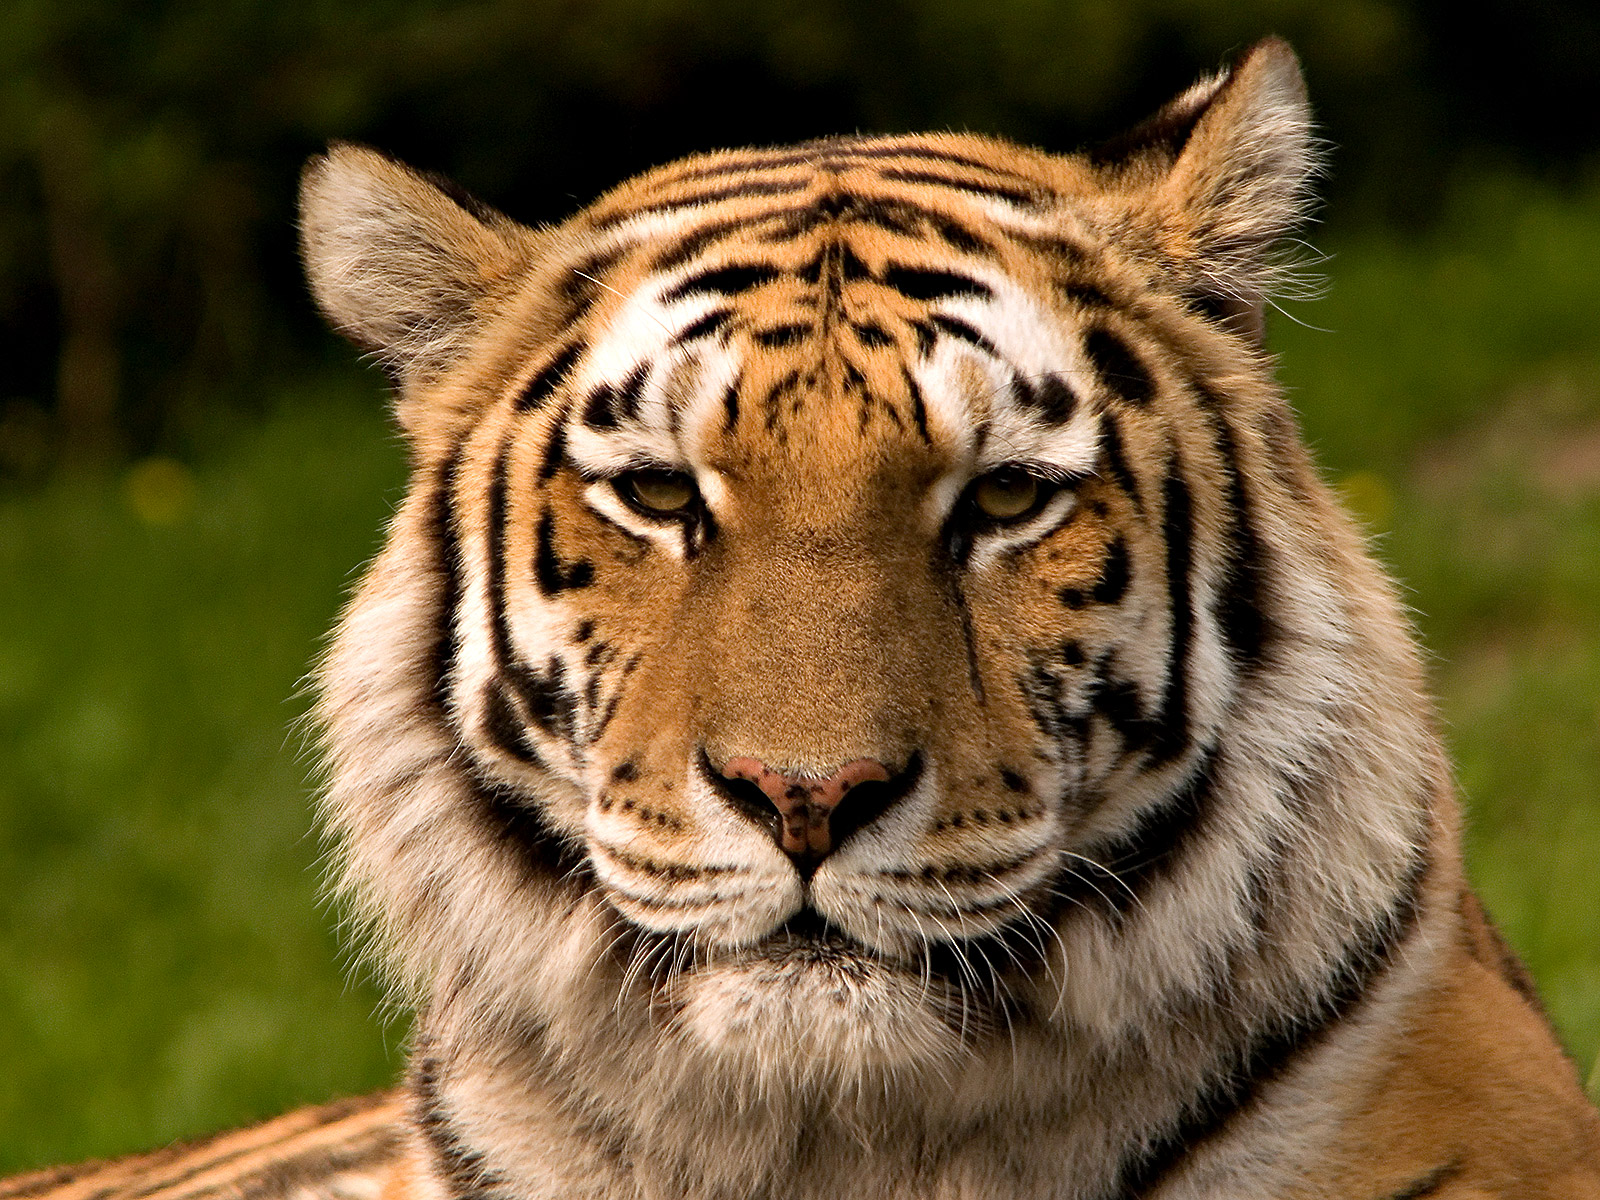
\includegraphics[width=0.5\textwidth]{fig/tiger.jpeg}
    \caption{\label{fig:tiger}A picture of a tiger.}
\end{figure}

Figure~\ref{fig:tiger} is a picture of a tiger.


%==========================================================================================
\subsection{Table}
\label{ss:Table}

\href{http://en.wikibooks.org/wiki/LaTeX/Tables}{Table examples on WIKIBOOKS}.

\begin{table}[htpb]\begin{center}
\caption{Table Example 1}
\begin{tabularx}{8cm}{llX}
\hline
Start & End  & Character Block Name \\
\hline
3400  & 4DB5 & CJK Unified Ideographs Extension A \\
4E00  & 9FFF & CJK Unified Ideographs \\
\hline
\end{tabularx}
 \end{center}\end{table}

\begin{table}[htpb]\begin{center}
\caption{Table Example 2}
\begin{tabular}{llr}
\hline
\multicolumn{2}{c}{Item} \\
\cline{1-2}
Animal & Description & Price (\$) \\
\hline
Gnat  & per gram & 13.65 \\
      & each     &  0.01 \\
Gnu   & stuffed  & 92.50 \\
Emu   & stuffed  & 33.33 \\
Armadillo & frozen & 8.99 \\
\hline
\end{tabular}
 \end{center}\end{table}
 
 \begin{table}[htpb]\begin{center}
	\label{t:prefix-table}
	\caption{Table Example 3}
	\renewcommand{\arraystretch}{1.0}
	\begin{tabularx}{300pt}{|c|X| }
		\hline
		\multirow{1}{*}{\textbf{Allocation}} &
		Allocation, Element, Type, Script 
		\\ \hline\hline
		%------------------------------
		\multirow{6}{*}{\textbf{Data Types}} &
        Byte2, Byte3, and Byte4\\ &
        Float2, Float3, Float4\\ &
        Int2, Int3, Int4\\ &
        Long2, Long3, Long4\\ &
        Matrix2f, Matrix3f, Matrix4f\\ &
        Short2, Short3, Short4
        \\ \hline\hline
		%------------------------------
		\multirow{4}{*}{\textbf{Graphics}} &
		Mesh\\&
		ProgramFragment, ProgramRaster\\&
		ProgramStore, ProgramVertex\\&
		RSSurfaceView
		\\ \hline
		%------------------------------
	\end{tabularx}
\end{center}\end{table}

\begin{table}[htpb]\begin{center}
\caption{Table Example 4}
\begin{tabular}{|l|l|l|}
\hline
\multicolumn{3}{|c|}{Team sheet} \\
\hline
Goalkeeper & GK & Paul Robinson \\ \hline
\multirow{4}{*}{Defenders} & LB & Lucus Radebe \\
 & DC & Michael Duberry \\
 & DC & Dominic Matteo \\
 & RB & Didier Domi \\ \hline
\multirow{3}{*}{Midfielders} & MC & David Batty \\
 & MC & Eirik Bakke \\
 & MC & Jody Morris \\ \hline
Forward & FW & Jamie McMaster \\ \hline
\multirow{2}{*}{Strikers} & ST & Alan Smith \\
 & ST & Mark Viduka \\
\hline
\end{tabular}
 \end{center}\end{table}
 
 \begin{table}[htpb]\begin{center}
\caption{Table Example 5}
 \begin{tabular}{l*{6}{c}r}
Team              & P & W & D & L & F  & A & Pts \\
\hline
Manchester United & 6 & 4 & 0 & 2 & 10 & 5 & 12  \\
Celtic            & 6 & 3 & 0 & 3 &  8 & 9 &  9  \\
Benfica           & 6 & 2 & 1 & 3 &  7 & 8 &  7  \\
FC Copenhagen     & 6 & 2 & 1 & 2 &  5 & 8 &  7  \\
\end{tabular}
 \end{center}\end{table}

%==========================================================================================
\subsection{Verb}
\label{ss:VerbUsage}
Let's take a overview on how to type special characters:\\
\verb|<FRAMEWORKS_BASE>/graphics/java/android/renderscript|\\\footnote{Path of <APP\_intermediates>: <ANDROID\_ROOT>/out/target/common/obj/APPS/APPNAME\_intermediates/}
You could also go back to the beginning of the chapter by the \hyperref[c:GetStarted]{\textbf{hyperref}}.

%==========================================================================================
\subsection{Enumeration}
\label{ss:Enumeration}
\begin{enumerate}
\item Enumerated Item1
\item Enumerated Item2
\item Enumerated Item3
\end{enumerate}

%==========================================================================================
\subsection{Code Display}
\label{ss:CodeDisplay}

\lstset{
	language=C++,
	stringstyle=\rmfamily,
	commentstyle=\itshape\color[rgb]{0.133,0.545,0.133},
	showstringspaces=false,
	basicstyle=\ttfamily\scriptsize,
	numberstyle=\tiny,
	numbers=left,
	stepnumber=1,
	numbersep=10pt,
	tabsize=2,
	breaklines=true,
	prebreak = \raisebox{0ex}[0ex][0ex]{\ensuremath{\hookleftarrow}},
	breakatwhitespace=false,
  	columns=fixed,
  	upquote=true,
  	extendedchars=true,
	xleftmargin=2em,
	xrightmargin=.5em,
	escapeinside={(*@}{@*)},
    mathescape=false,
}
Here is a "Hello, DanDing." example:
\begin{lstlisting}[style=nonumbers] 
void main(int argc, char **argv)
{
    printf("   ˊ_> ˋ  ");
}
\end{lstlisting}


Another example with line numbers:
\begin{lstlisting}
void main(int argc, char **argv)
{
    printf("   ˊ_> ˋ  ");
}
\end{lstlisting}

Matlab example:

\definecolor{dkgreen}{rgb}{0,0.6,0}
\definecolor{gray}{rgb}{0.5,0.5,0.5}
\lstset{language=Matlab,
   keywords={break,case,catch,continue,else,elseif,end,for,function,
      global,if,otherwise,persistent,return,switch,try,while},
   basicstyle=\ttfamily,
   keywordstyle=\color{blue},
   commentstyle=\color{red},
   stringstyle=\color{dkgreen},
   numbers=left,
   numberstyle=\tiny\color{gray},
   stepnumber=1,
   numbersep=10pt,
   backgroundcolor=\color{white},
   tabsize=4,
   showspaces=false,
   showstringspaces=false}

\begin{lstlisting}
function y = demo(x) % This is a comment.
   str = 'hello there';
   y = x + 1;
end
\end{lstlisting}

%==========================================================================================
\subsection{Math}
\label{ss:Math}
\begin{itemize}
    \item Inline mode:\\
The solution to $\sqrt{x} = 5$ is $x=25$.
    \item Display mode:\\
The solution to \[\sqrt{x} = 5\] is \[x=25.\]
    \item Numbered mode:
\begin{equation}
2+2=4
\end{equation}
    \item Non-numbered:
\begin{equation*}
2+2=4
\end{equation*}
    \item Aligning:
\begin{align*}
2x^2 + 3(x-1)(x-2) & = 2x^2 + 3(x^2-3x+2)\\
&= 2x^2 + 3x^2 - 9x + 6\\
&= 5x^2 - 9x + 6
\end{align*}
     \item Fractions:
\[
 \frac{n!}{k!(n-k)!} = \binom{n}{k}
\]
    \item Matrix:
\[
 A_{m,n} =
 \begin{pmatrix}
  a_{1,1} & a_{1,2} & \cdots & a_{1,n} \\
  a_{2,1} & a_{2,2} & \cdots & a_{2,n} \\
  \vdots  & \vdots  & \ddots & \vdots  \\
  a_{m,1} & a_{m,2} & \cdots & a_{m,n}
 \end{pmatrix}
\]
\end{itemize}
\href{http://en.wikibooks.org/wiki/LaTeX/Mathematics}{More examples on WIKIBOOKS}.


%==========================================================================================
\subsection{Algorithms}
\label{ss:Algorithms}
\begin{algorithm}[h]                      % enter the algorithm environment
\caption{Calculate $y = x^n$}          % give the algorithm a caption
\label{alg1}                           % and a label for \ref{} commands later in the document
\begin{algorithmic}                    % enter the algorithmic environment
    \Require $n \geq 0 \vee x \neq 0$
    \Ensure $y = x^n$
    \State $y \Leftarrow 1$
    \If{$n < 0$}
        \State $X \Leftarrow 1 / x$
        \State $N \Leftarrow -n$
    \Else
        \State $X \Leftarrow x$
        \State $N \Leftarrow n$
    \EndIf
    \While{$N \neq 0$}
        \If{$N$ is even}
            \State $X \Leftarrow X \times X$
            \State $N \Leftarrow N / 2$
        \Else[$N$ is odd]
            \State $y \Leftarrow y \times X$
            \State $N \Leftarrow N - 1$
        \EndIf
    \EndWhile
\end{algorithmic}
\end{algorithm}
\href{http://en.wikibooks.org/wiki/LaTeX/Algorithms_and_Pseudocode}{More examples on WIKIBOOKS}.


\chapter{Introduction}
\label{c:intro}

There can be million lines of code in today's software system.
On such a scale of complexity, defects in the source codes are unavoidable.  
Various empirical studies show that the defect density of commercial software system is around 1 to 20 defects in every 1000 lines of source code\cite{Sommerville:2006:SE:1196763}.
Therefore, developers of systems created many engineering techniques to contain the damage that could be caused by such defects.
For example, a software system may have several measures to its disposal to avoid system failure, including resending the request, resetting the server, clearing the communication buffers, and etc when observing that a critical service request is not acknowledged.
However, in general, since all the recovery cost time and money it is important to estimate how to organize the measures for the maximal resilience of the system against realistic errors.
At the moment, an automated support which can suggest defence techniques to development teams is missing.
I created a game theoretic approach to study this problem and carried out experiments to show how this approach can be helpful in  synthesizing the most resilient defence of software systems against multiple errors.

The naive way to measure the safety level of a system is to find the number of errors that it can endure before running into failure state.
But in second thought, no non-trivial system can handle unlimited errors without degrading to inevitable system failure.
Thus, it would be meaningless to analyse the resilience level of the systems to software errors can proceed without creating a realistic error model in which practical control mechanism can be devised to defend the systems against errors.
In this work, I am interested in defending the system against a more restricted error model, but still let the error model has a quantifiable level of power in order to simulate different error scenarios.
Further more, I think a reasonable foundation need to take into consider that the life-time of a software system is much longer than the duration needed for a reasonably designed software system to recover from an error.
Therefore, I propose to evaluate control mechanism of software systems on how many errors the control can endure before recovery to safe states.
I then present an algorithm to find a control strategy that can handle the maximum number of such errors.

Let us standardize the basic terms before proceeding further.
A design defect in software or hardware is called a {\it fault} in embedded systems.
An {\it error} (sometimes called component failure in the literature) is the effect of a fault that causes a difference between the expected and the actual behavior of a software system, e.g., measurement errors, read/write errors, etc. 
An {\it error} does not always lead to a system failure, but may instead be repaired by, e.g., a defence mechanism in the software. 
That is, an {\it error} may be detected and fixed/neutralized before it creates any harm to the system or its users.
A {\it failure} is the fact that users can observe the faulty behavior created by {\it errors}.

My specific goal is to develop a technique for finding a control mechanism of a software system which can against the maximal number of dense errors without degrading to failure.
My inspiration is from methods for resilient avionic systems\cite{conf/ftrtft/Rushby92}, where fault tolerance is designed to recover from a bounded number of errors.
The number of errors a system needs to tolerate is calculated from the mean time between errors of individual components and the maximal duration of the system.
I use the quality guarantees one obtains for an airplain(the system) as an example to demonstrate the difference between the objective to tolerate up to {\it k errors} and sequences of separated blocks of up to {\it k dense errors} in a short period.
Assuming the operating time of the system is 20 hours, the mean time between exponentially distributed errors is 10 hours and the repair time is 3.6 seconds.
The mean time between dense errors (consecutive errors before system recovery) is calculated in Table~\ref{tab.mtbf}.
\begin{table*}
\begin{center}
\begin{tabular}{l||c|c|c|c|c|c|c|c}\hline 
$k$              & $0$     & $1$     &    $2$   &  $3$  & $4$ & $5$ & $6$ & $\ldots$ \\\hline 
$k$ errors       & $0.865$ & $0.594$ & $0.333$ & $0.143$ & $0.053$ & $0.017$ & $0.005$ & $\ldots$ \\
$k$ dense errors & $0.865$ & $2 \cdot 10^{-4}$ & $2 \cdot 10^{-9}$ & $2 \cdot 10^{-14}$ & $2\cdot 10^{-19}$ & $2\cdot 10^{-24}$ & $2\cdot 10^{-29}$ & $\ldots$ 
\\ \hline 
\end{tabular}
\end{center}
\caption{Probabilities of $k$ dense errors} 
\label{tab.mtbf} 
\end{table*} 
%\bibliographystyle{unsrt}
%\bibliography{thesisbib}
The figures for $k$ errors (component failures) are simply the values 
for the Poisson distribution with coefficient $2$.
To explain the figures for $k$ dense errors, 
consider the density of 2 dense errors occurring in close succession.
If an error occurs, the chance that the next error occurs 
within the repair time (3.6 seconds) is approximately $\frac{1}{10000}$.
The goal to tolerate an arbitrary number of up to $k$-dense errors is, of course, 
much harder than the goal of tolerating up to $k$ errors, but, 
as the example shows, the number $k$ can be much smaller.   
Tolerating an arbitrary number of errors 
(with a distance of at least $3.6$ seconds between them) 
creates the same likelihood to result in a system failure 
as tolerating up to $9$ errors overall, and 
tolerating up to $15$ errors still results 
in a $70\%$ higher likelihood of a system failure 
than tolerating blocks of up to $2$ errors in this example. 
Only errors for which this is the case could cause a system failure.
The mean time between blocks of two dense errors is therefore not ten hours, 
but 100,000\label{reply2.100000} hours.
Likewise, it increases to 1,000,000,000 (one billion) hours for blocks of three dense errors, and so forth.

Maximizing the number of dense errors that are permitted before full recovery 
is therefore a natural design goal.  
After full recovery, the system is allowed again the same number of errors.
Now, if the {\em mean time between errors} ({\em MTBE}) 
is huge compared to the time the system needs to fully recover, 
then the mean time between system failures (MTBF) grows immensely. 

We view the problem of designing a resilient control mechanism 
towards dense errors as a two-player game, 
called {\em safety resilience game}, 
between the system (\label{reply1.protagonist.player1}protagonist\footnote{In game theory, a protagonist sometimes is also called {\em player 1}.}, `he' for convenience) 
and a hostile agent (antagonist\footnote{In game theory, an antagonist sometimes is also called {\em player 2}.}, `she' for convenience) 
that injects errors into the system under execution.\label{reply1.antagonist.inject.errors}   
The protagonist wants to keep the system from failure in the presence of errors, 
while the antagonist wants to derail the system to failure. 
\label{reply1.how.models} 
Specifically, 
system designers may model their system, defense mechanism, and error model 
as a finite game graph.  
The nodes in the graph represent system states.
These system states are partitioned into three classes:
the safe states, the failure states, and the recovery states. 
Some transitions are labeled with errors while others are considered normal transitions.  
The game is played with respect to a resilience level $k$.  
If a play ever enters a failure state, then the antagonist wins in the play.  
Otherwise, the protagonist wins.

The protagonists plays by selecting a move, intuitively the `normal' event that should happen next (unless an error is injected).
The antagonist can then decide to trigger 
an error transition (injecting an error) with the intention to
eventually deflect the system into a failure state. 
Our error model, however, restricts 
the antagonist to inject at most $k$ errors before she allows for a long period of time that the system may use to recover to the safe states.
(If the antagonist decides to use less than $k$ errors, the protagonist does not know about this.
It proves that this information is not required, as we will show
\label{reply1.memoryless.future} that the protagonist can play memoryless.)
After full recovery by the protagonist to the safe states, the antagonist is allowed again 
to inject the same number of errors, and so forth.
  
If the system can win this game, then the system is called {\em $k$-resilient}.
For $k$-resilient systems, there exists a control strategy---even one that does not use memory---to make the system 
resilient in the presence of blocks of up to $k$ dense errors. 
We argue that, if the component MTBF is huge compared to the time the system needs to fully recover, then the expected time for system breakdown grows immensely.  

Besides formally defining safety resilience games, we also present algorithms 
for answering the following questions.  
\label{reply2.alg.sfrch.res}
\begin{itemize} 
\item Given an integer $k$, a set $F$ of failure states, and 
  a set $S$ of safe states (disjoint from $F$), is there a recovery mechanism that 
  can endure up to $k$ dense errors, 
  effectively avoid entering $F$, and quickly direct the system back to $S$.  
  Sometimes, the system designers may have designated parts of the state space 
  for the recovery mechanism.  
  The answer to this question thus also implicitly tells 
  whether the recovery 
  mechanism is fully functional in the recovery process. 
\item Given an integer $k$ and the set of failure states, 
  what is the maximal set of safe states, 
  for which the system has a strategy to maintain $k$-resilience?
  In game theory, this means that 
  safety resilience games can be used for synthesizing safety regions 
  for a given bound on consecutive errors before the system is fully recovered.  
  
The question can be extended to not only partition the states into safety, recovery, and failure states, but also for providing memoryless control on the safety and recovery states.
  
\item Given a set of failure states, what is the maximal resilience level of the system that can be achieved with proper control?  
  We argue that this maximal resilience level is a well-defined and plausible indicator of 
  the defense strength of a control mechanism against a realistic error model. 
\end{itemize} 
With our technique, 
software engineers and system designers 
can focus on maximizing the number of dense errors that 
the system can tolerate infinitely often, providing that they are grouped into blocks that are separated by a short period of time, which is sufficient for recovery.

We investigate how to analyze the game with existing techniques. 
We present an extension to alternating-time $\mu$-calculus (AMC) 
and propose to use the AMC model-checking algorithm on concurrent games to check 
resilience levels of embedded systems. 
We present reduction from safety resilience games to 
AMC formulas and concurrent game structures.  
Then we present a PTIME algorithm for answering whether the system can be 
controlled to tolerate up to a given number of dense errors.  
The algorithm can then be used to find the maximal resilience level 
that can be achieved of the system. 
The evaluation is constructive:  
it provides a control strategy  
for the protagonist, which can be used to control a system 
to meet this predefined resilience level.  


\chapter{Software Resilience against Dense Errors}
\label{c:resilience}




\section{Two-player concurrent game structures}
To facilitate our explanation of resilience analysis in a game's 
perspective, 
we start by reviewing the game concepts related to our work. 
A concurrent game may involve several players\label{reply1.multiple.players}, who make concurrent move decisions at the same time during transitions. 
The destination of a transition is jointly determined by the moves chosen by all players.  
Such a game model is very expressive and handy in 
describing interactions in a complex system.  
In this work, we adapt the finite concurrent games from \cite{AHK02} 
with event concepts on transitions.  
For the analysis of system resilience, 
we only have to consider two players in the game, 
the first is the system, and the second is the error model. 


\begin{definition} \label{def.cncgame} 
{\bf (2-player concurrent game structure):}
A {\em concurrent} game structure is a tuple 
$\calk=\langle Q,r,P,\lambda,E_1,E_2,\delta\rangle$, where
\begin{list1}
\item $Q$ is a finite set of states. 
\item $r$ is the initial state in $Q$.  
\item $P$ is a finite set of atomic propositions. 
\item $\lambda:Q\mapsto 2^P$ is a proposition-labeling function of the states. 
\item $E_1$ and $E_2$ are finite sets of move symbols that the protagonist and 
the antagonist can respectively choose in transitions.  
A pair in $E_1\times E_2$ is called a {\em move vector}.  
\item $\delta$ is a function that maps 
  from $Q\times E_1\times E_2$ to $Q$.  
  $\delta$ is called the transition function and 
  conceptually specifies a successor state 
  that results from a state and moves of the players. 
%   For convenience, we require that every state has a successor state. 
\label{reply1.for.convenience.succ} 
\end{list1}
Given a state $q\in Q$ and a vector $[e_1,e_2]\in E_1\times E_2$, 
$\delta(q,e_1,e_2)$ is the successor state from 
$q$ when each player $a\in \{1,2\}$ chooses her respective move $e_a$.  
\qed 
\end{definition} 

We prefer to represent the moves available to the players by symbols (rather than integers as in \cite{AHK02}), as move (or event) symbols can be used to reflect some physical meaning.  
For example, a move can correspond to the turning-off of a switch,  
the detection of an airplane, 
or\label{reply1.grammar.or} the execution of an error handling routine.  
(Technically, representing moves as either integers or symbols 
does, of course, make no difference.)


\section{Motivation}
\subsection{Background}
Resilience to errors in computer systems is\label{reply2.are.is} usually 
achieved through error recovery design as illustrated in Figure~\ref{fig.frwk}.  
%\begin{figure}[t]
%\begin{center}
%\epsfig{file=state-par.eps,width=60mm}
%\caption{Framework of resilience design}
%\label{fig.frwk} 
%\end{center}
%\end{figure}  
The system states can be partitioned into three regions: 
safe, recovery, and failure. 
The left part of the figure represents the safety region.
The states in this safe region can be viewed as those for `normal' operation. 
When an error occurs, the system goes through a recovery stage, where it follows some recovery mechanism.
This is shown as the ``recovering'' area in Figure~\ref{fig.frwk}.
In this region, the system intuitively tries to repair the effects of an error and thus to recover to the safety region. 

During the recovery (or: in the recovery region), however, errors may still happen.  
In general, fault-tolerant systems are built under the assumption that error detection and recovery is speedy and that there 
% cannot be too many errors 
can only be a few errors\label{reply2.cannnot.be2} 
during the process of recovery.
If the recovery mechanism is not resilient enough, a few errors may drive the system into failure.  

We illustrate this on the following examples.  

\begin{example} 
{\bf (Fault-tolerant computer architectures):}  
\label{exmp.avi}
In computer architectures, 
fault-tolerance is usually achieved via hardware duplication.  
Consider an example of a multi-processor system that
includes $n$ processor copies and $m$ memory copies.  
The $n$ processors each can follow the instructions
of the original system, or be engaged in memory recovery. 
When a copy of the memory fails, a processor can be assigned to recover it.
Majority check can be used to detect that a processor is faulty
or that memory copy is faulty\label{reply2.defected} (often, both would happen at the same time). 
For recovery, we can set a free processor to recover some memory copy, or
make a processor follow the code of the majority of processors.

The key to error resilience is to decide whether to make
a processor follow the execution of the majority, or to
assign it to recover faulty memory. 
If too many errors occur in a short while before 
the errors can be recovered from, 
then there may be no more processors left to carry out any more recovery. 
When such a critical situation arises, the system enters failure state when another error is induced.  

The recovery mechanism described\label{reply2.in.the.above} above is typical in 
the design of fault-tolerant systems \cite{Pradhan96}.  
As explained, a practical recovery mechanism usually 
does not rely on the detailed structure of the system.  
Instead, error-detection 
techniques such as parity checks, voting (for majority checks), 
etc., are usually employed.  
In fact, the number of duplicates is usually\label{reply2.usually.is} critical to the 
resilience of the system to errors. 
As long as the majority of the duplicate modules can be recovered 
in time (i.e., before the\label{reply2.the.next} next wave of errors), 
resilience of the system can be achieved. 
\qed 
\end{example} 

\begin{example} {\bf (Exception handling):} 
\label{exmp.ehan} 
At the operating system level, errors are usually signaled via 
interrupt lines and handled with routines called handlers.  
The first thing that needs~\label{reply2.needs.to} to be done by a handler is to save 
the CPU state of the interrupted process. 
In some operating systems, a static memory space is used for 
this purpose for each handler. 
In such a scheme, if the same error happens again while executing 
the error handler, then the system can run into the risk that 
the CPU states of the interrupted handler can be overwritten and 
destroyed. 

Another scheme is to use a stack to save the CPU states of the interrupted 
processes.  
Such a scheme seems resilient to errors that happen during\label{reply1.durin1} the execution of 
error handlers.  
Still, too many errors that happen during the execution of error handlers
can deny critical functions\label{reply2.delay.timely} of the system and 
incur failures, including missed timer updates and priority inversions.   
Thus, a proper assumption on the timely error recovery by 
the error handling routines is critical to the design of 
error resilience in such cases.  
\qed 
\end{example} 

\begin{example} {\bf (Security attacks):} 
\label{exmp.satt}
Security in the Internet also relies on resilience to attacks 
of hackers, viruses,\label{reply2.viruses} malware, etc.  
For example, one common technique of attacks\label{reply2.attacks} 
to communication modules is to 
overflow the communication buffers.  
In such attacks, the sizes\label{reply2.sizes} of the buffers and the ability 
of the security procedures to detect and recover 
from such overflowing attacks is crucial to the resilience design.  
\qed 
\end{example} 

%% >>> changes start 
These examples show that recovery is a crucial concept for\label{reply2.in2for} designing systems 
that are resilient to errors. 
When system errors are detected in such a system, 
the system activates a recovery mechanism so as to remove the effect of the errors. 
When designing such systems,\label{reply2.such.systems} the system designers usually
have in mind 
what errors and failures the systems can expect, according to the specification.  
\label{reply2.comparatively}
To avoid failures in the occurrence of dense errors, the system designers usually incorporate many error recovery mechanism 
in the system, e.g., exception handlers and hardware/software redundancy. 
But, in general, it would be difficult for the designers to evaluate 
how effective their recovery mechanism is to dense errors.  
To overcome this difficulty, we believe that it is important to 
support them with automated analytical tools with a solid foundation.  

Resilience has also been used in \cite{EhlersT14,BloemEJK14} with a similar goal.
When synthesising code, one relies on assumptions of the behavior of the environment, and the formal specification\label{reply1.speicification} would only ask for the provision of guarantees under the condition that the assumptions are satisfied.
When assessing the quality of an implementation, the behavior in cases\label{reply1.cases.comma} where the environment does not comply with the assumption matters.
In \cite{EhlersT14,BloemEJK14}, the resilience model we have introduced in the conference version \cite{HPSW/12/rapidRecovery} 
of this paper\label{reply1.of.this.paper}
has been followed up upon, and proven to be well suited for reactive synthesis.

In this work, we use these observations to design \label{reply1.theoretical.framework.eval} 
a theoretical framework for synthesizing a control mechanism that provides 
the maximal resilience against software errors in a realistic error model.
\subsection{Resilience in a Nutshell}
\label{reply2.from.the.examples} 
From Example~\ref{exmp.avi} to \ref{exmp.satt} in 
Subsection~\ref{subsec.rgame.bkg}, it is easy to see 
the common paradigm of error recovery in software systems.  

\begin{quote}
When errors are detected, a recovery mechanism will be activated
to avoid failures and try to get back to normal execution. 
\end{quote}

Moreover, \label{reply1.a.recovery.the.assumption}
such a recovery mechanism usually needs to operate under the assumption 
that more errors may also happen during the recovery process. In practice, system designers have already implemented many defensive modules, 
e.g., exception handlers, which are certainly good candidates for the recovery segments.  
Thus, the recovery scheme we discuss is likely to have arisen in an ad-hoc fashion as a natural concept when software architects and programmers designed recovery mechanisms for critical software.  

The vast state spaces of critical systems make an automated support for and a solid foundation 
of evaluating design alternatives particularly valuable. 

In the following, we will use the examples from the previous subsection 
as a motivation for defining a new game, called {\em safety resilience game}, 
between the recovery mechanism (the protagonist) 
and the error-injecting agent (the antagonist).  
\label{reply2.S.F}
The game is specified with a set $F$ of failure states, 
a set $S$ of safe states (the safety region), the 
moves by the antagonist to inject errors, 
and the resilience level $k$ that the designers want to achieve. 
The objective of the protagonist is to identify a control strategy 
so that the whole system can achieve the prescribed level (or 
the highest level) $k$ of resilience for safety region $S$ (a set of states) 
and failure state set $F$.  

The game is played round by round. 
When the antagonist issues an error move, 
the play may be deflected into a recovery segment.  
If there are no more than $k-1$ errors in the recovery segment, 
then a $k$-resilient control mechanism must direct the recovery segment
to end at a safe state. 
The above observation suggests that 
a safety region can be abstracted as a fixed point 
to the recovery procedure 
that transforms a safe state to another safe state via the recovery segment 
with at most $k-1$ errors. 
\label{reply1.fixed.point.explanation} 
Conceptually, a fixed point to a procedure $f(x)$ is a set $S$ of elements 
in the domain of $x$ such that $S=\{f(x)\mid x\in S\}$.  
To calculate the fixed point of the recovery procedure, 
we can use the greatest fixed point algorithm.  
The idea is to start from a superset of the recovery procedure fixed point. 
For convenience, we call a superset of the fixed point a {\em pseudo fixed point} 
({\em PFP}).  
Then we iteratively check every state $q$ in the PFP and eliminate 
$q$ from the PFP if, after at most $k$ errors from $q$, 
the recovery mechanism either cannot avoid failure or 
cannot direct the system back to the PFP. 
As the iterative checking and elimination goes on, 
the PFP will shrink and eventually stabilize.
Note that its size is always finite, 
since the initial PFP must be no bigger than $Q$.  
The final PFP is then a greatest fixed point to the recovery mechansim for 
$k$-resilience and is the legitimate safety region.  
 

This recovery procedure can be illustrated as in Figure~\ref{fig.sfrch} 
for resilience to $2$ errors.  
%\begin{figure}[t]
%\begin{center}
%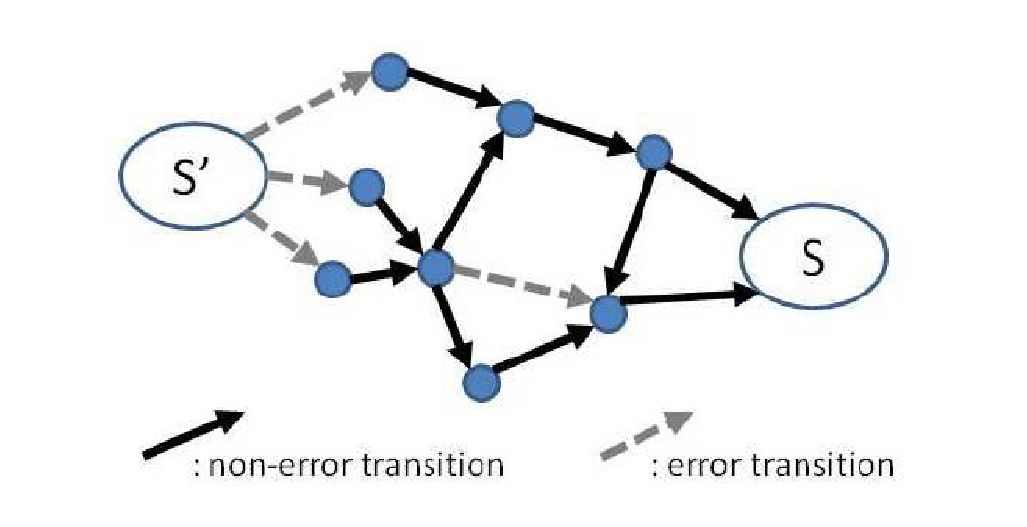
\epsfig{file=rseg.eps,width=60mm}
%\caption{Illustration of the recovery operation}
%\label{fig.sfrch} 
%\end{center}
%\end{figure}  
In this figure, the states in set $S'$ are computed  
as the precondition of states in $S$ through those transitions in the figure.  
Each path from $S'$ to $S$ is a recovery segment. 
$S$ and $S'$ may overlap.  
The blue circles represent states in the recovery segments.  
If we calculate $S'$ out of $S$, 
then, for each state $q'\in S'$, we can find a path from 
$q'\in S'$ via a path in the recovery segment to another state $q\in S$.  
The maximal number of errors in a recovery segment is 2.  
Thus the protagonist has a strategy to recover from errors in $S'$ to $S$ 
even when 2 errors happen in the corresponding recovery segment.  
When $S'=S$, then $S$ is a fixed point to the precondition 
operator through the recovery segments in the figure.  

Now we formally define the concept that we explained with Figure~\ref{fig.sfrch}.  

\begin{definition}{\bf ($k$-safety):} 
\label{k-safe}
Given a $k\in\nnneg$, 
a state $q$ is called \mbox{$k$-safe} with respect to 
a safety region $S\subseteq Q\smallsetminus F$ of non-failure states, 
denoted $q\in\safe_k(S)$, if there 
is a strategy for the protagonist to guarantee that 
we can reach back to $S$ from $q$, provided that
the overall count of errors is at most $k$.
\qed 
\end{definition}

However, the definition can be subtle in its interpretation.  
Specifically, the ability to stand against one wave of $k$ errors 
is not the same as that against repeated recovery 
from waves of $k$ errors.  
If the recovery mechanism is not designed properly, 
the system may gradually lose a bit of control after each wave of $k$ errors 
and eventually degrade to system-level failure. 

\begin{example} 
{\bf (Fault-tolerant computer architectures):}  
\label{exmp.avi.revisit}
Consider Example~\ref{exmp.avi} with $2k+1$ processor copies, 
with the objective to maintain majority checks
and to identify the bad processors. 
Indeed, according to the first, na\"ive solution, 
any safe state with a recovery strategy to 
$Q\smallsetminus F$ is good.   
After $k$ processor copies fail, 
the majority checks are still capable to maintain the correctness
of the combined behavior to follow the design of the original system.  
There seems to be nothing to do after $k$ errors.  
Thus, na\"ively, we can choose those states as the safety region
\label{reply1.majority.checks.as.safety.regions} if, 
at those states, majority checks still work.  

However, there is no expectation that the system will be able
to recover at any point in the future into a situation where it can bear 
another wave of $k$ errors.   
It will fail and lose the function of majority checks just after one more error.  
In contrast, in this work, we aim to propose a dense error resilience criterion that 
given no more errors for enough time to allow recovery, 
the system will eventually recover to resilience to $k$ dense errors again. 
%Note that `enough time' is a system parameter that refers to the time required for recovery, provided no further errors occur.
\qed 
\end{example} 

To look at this issue in more detail, 
please consider the transition system with four states, 
including a single failure state
(state $4$, marked by a double line) shown in Figure~\ref{fig:example}.
The controlled transitions are depicted as black solid arrows, 
the error transitions are depicted as red dashed arrows.
For $S=Q\smallsetminus F=\{1,2,3\}$, all states in $S$ are in $\safe_0(S)$.
For all $k \geq 1$, we have $\safe_k(S)=\{1,2\}$:
the protagonist can simply stay in $\{1,2\}$ 
during the safety phase of the game, and once the antagonist 
plays an error transition, the game progresses 
into the recovery segment, where the protagonist's objective 
is satisfied immediately.
This outlines the difference between $k$-sfrch-ty and 
the linear time property
of being able to repeatedly tolerate waves of up to $k$ errors, 
which would only be satisfied by states $1$ and $2$ for 
$k = 1$, and only for state $1$ for $k = 2$.



\begin{figure}[t]
\begin{center}
\psset{xunit=26mm,yunit=7mm}
\begin{pspicture}(0,-.15)(3,1.4)
% \pnode(0,.6){0}
\rput(0,0){\circlenode{1}{$1$}}
\rput(1,0){\circlenode{2}{$2$}}
\rput(2,0){\circlenode{3}{$3$}}
\rput(3,0){\circlenode[doubleline=true]{4}{$4$}}
% \ncline{->}{0}{1}
\nccircle{->}{1}{.35}
\nccircle{->}{2}{.35}
\nccircle{->}{3}{.35}
\ncarc[linecolor=red,linestyle=dashed]{->}{1}{2}
\ncarc{->}{2}{1}
\ncarc[linecolor=red,linestyle=dashed]{->}{2}{3}
\ncarc{->}{3}{2}
\ncline[linecolor=red,linestyle=dashed]{->}{3}{4}
\end{pspicture}
\end{center}
\caption{\label{fig:example} An example for calculating $\safe_k$}
\end{figure}




This difference raises the question 
if the rules of our game are depriving the antagonist 
of some of the $k$ errors that she should intuitively be allowed to insert in a wave.
The answer is that this is not the case 
if we use any fixed point of $\safe_k$ as $S$.
In this case, the protagonist would regain the capability to endure a wave of $k$ errors when reaching a safe state after recovery.
Instead of depriving the antagonist, 
one could say that we reset the number of errors in any recovery 
segment that the antagonist can inject to $k$.
Thus such a fixed point of $\safe_k$ should consist of 
states, from which we can use a control mechanism to fend off 
repetitive waves of $k$ dense errors in the recovery segments.  
For convenience, we call states in such a fixed point of $\safe_k$  
the $k$-resilient states. \label{reply1.k.resilient.states}  

% Thus, we can simply define the set of $k$-resilient states while the definition of $k$-sfrch-ty does not demand that the 
% system tries to recover, given enough 
% game steps, into a state where it can sustain more failures,
% for $k$-resilience, after recovery, $k$ more failures should be allowed, and so forth.
% Resilience is similar to the property of `home states', 
% where the system is capable, given enough time and 
% no interruption (in the form of failures), 
% of reaching again the good situation where it is again resilient to 
% $k$ failures.

For a state to be in $\safe_k(S)$, 
the system (protagonist) has a strategy to recover to $S$, 
given that a long enough execution commenced 
without another round of $k$ errors happening.
We say that two successive errors are in the same 
\emph{group of dense errors} 
if the sequence of states separating them 
was not long enough for recovery to the safety region.
Vice versa, if two successive errors are far enough apart 
such that the protagonist can guarantee recovery in this separation, 
then they do not belong to the same group.
% (Besides the practical motivation of what recovery encounters in our examples, this assumption also has the technical motivation that memoryless strategies suffice for the protagonist to win $\safe_k(G)$.)
% 
% A state is $k$-resilient if groups of up to $k$ dense failures can be tolerated infinitely many times, provided that the system is given enough time to recover;
% $k$-sfrch-ty is equivalent to tolerating up to {\em one} set of $\leq k$ dense errors%
% \footnote{Note that the technical definition of sfrch states implies that a set of dense errors ends once the protagonist has recovered to $G$.
% Thus, as seen in the example, a state from which no two failures can be tolerated might be $k$-sfrch for all $k$.}.

To check whether recovering to $S$ by the protagonist (the fault-tolerance mechanism)
is always possible, provided that at most $k$ errors occurred during 
a recovery segment, observe that nesting 
$\safe_k$ once, i.e., $\safe_k(\safe_k(\cdot))$, corresponds
to tolerating up to two rounds of up to $k$ dense errors, and so forth.
Thus, for $S$ to be a target of recovery for $k$-resilience, 
$S$ must be a fixed point of the operator
$\safe_k$ from Definition~\ref{k-safe}, or, equivalently, 
$S=\safe_k(S)$ must hold.  
Moreover, if $S$ is the greatest fixed point to $k$-resilience, then we we can apply 
$\safe_k()$ any number of times to $S$ and still obtain $S$.  
Computationally, the greatest fixed point of $\safe_k$ can be constructed as 
by executing  
\begin{center} 
$\safe_k(\safe_k(\safe_k(\ldots\ \safe_k(S\big)\ldots)))$,
\end{center}  
using a sufficiently deep nesting that a fixed point is reached.

Note that this fixed point $x$ to $x=\safe_k(x)$ is what we are really interested in, 
while $\safe_k(S)$ for a given $S$ is an intermediate result that does not 
guarantee survival of the systems after waves of dense errors.
If this greatest fixed point
$$R = \bigcup\{X \subseteq S \mid X = \safe_k ( X )\}$$ is non-empty, 
the protagonist's strategy for 
the fixed point (guaranteeing eventual recovery 
to a state in the fixed point within no more than $k$ errors, i.e., $k$-resilience) 
can be used to control the recovery mechanism, 
constraining its transitions to follow its winning strategy.

As explained in the introduction, 
there can be several natural control problems in our safety resilience game.
First, the system designers may want to know whether the chosen safety region $S$ can 
be supported by the recovery mechanism for resilience level $k$.  
Second, they may want to get design support for choosing the safety region 
for achieving resilience level $k$.  
Finally, they may want to know the maximal resilience level that they can achieve. 


With the explanation in the above, in the rest of the manuscript, 
we will focus on the algorithm for constructing 
$\safe_k(\cdot)$ and evaluating $k$-resilient states. 



\section{Safety resilience games}
A system is $k$-resilient if it
can be controlled to tolerate infinitely many groups of up to $k$ dense errors, 
provided that the system is given enough time to recover between these groups.
As we have explained, in systems developed with defensive mechanism against errors,  
when errors are detected, recovery procedures should be activated.  
The major challenge is to decide given a set of failure states and a safety region,
whether 
the recovery mechanism can support a resilience level required\label{reply1.prescribed.2.required} by the users. 
Our goal is to develop techniques with a solid foundation to 
assist the system designers in evaluating the resilience of their systems, 
to synthesize the controller strategy for the required resilience level, and 
to achieve the maximal resilience level. 


We now formally define the safety resilience game played between a 
system (the protagonist) and an error-injector (the antagonist).  
Initially, the two players are given a 2-player concurrent game structure $\calk$,  
a pebble in $r$,  
a set $F\subseteq Q$ of failure states, and 
a safety region $S\subseteq Q\smallsetminus F$. 
Then the recovery region consists of states in $Q\smallsetminus (F\cup S)$.  
The two players together make decisions and move the pebble from state to state.   
The antagonist tries to deflect a play into $F$ by injecting sufficiently many errors, while
% On the other hand, 
the protagonist tries to avoid that the pebble reaches $F$. 
To achieve this, the protagonist can use the recovery region as the safety buffer and try to 
get back to $S$ as soon as the play is deflected from $S$ 
to the recovery region.  
If a system is resilient to $k$ errors, then it means that 
the protagonist can handle up to $k-1$ errors while in the recovery region.  
Thus when checking whether a system is resilient to $k$ errors, 
we only need to check those recovery segments with no more than $k-1$ errors. 

In the following, we formalize the concept.  

\begin{definition} \label{def.srgs} 
{\bf (Safety resilience game structure):} 
Such a structure is a pair $\langle \calk, F\rangle$ with the following 
restrictions. 
\begin{list1} 
\item $\calk$ is a 2-player concurrent game structure 
  $\langle Q,r,P,\lambda,E_1,E_2,\delta\rangle$.  
  Conceptually, the first player represents the system / the protagonist, while 
  the second player represents the error model / the antagonist.  
\item $E_2$ is partitioned into error and and non-error moves $E_{\emerr}$ and $E_{\emnerr}$, respectively.
%   The error moves are characterized by a condition `$\emerr$', while the non-error moves  are characterized by a condition `$\emnerr$'.
We require that only the 2nd player can issue $\emerr$ moves.  
Moreover, $E_{\emnerr}$ must be non-empty. 
\item $F$ is the set of failure states in $Q$ with $r\not\in F$.   
\end{list1} 


The antagonist can choose if she wants to respond on a move of the protagonist with an error move. \label{abstraction}
We allow for different non-error moves to reflect `normal' nondeterministic behavior, e.g., caused by abstraction. 
We allow for different error moves to reflect different errors that can occur in the same step.

We sometimes refer\label{reply1.reffer} to transitions with $\emerr$ moves by the antagonist as \emph{error transitions} and 
to transitions with  $\emnerr$ moves by the antagonist as \emph{controlled transitions}.  

For a party $A \subseteq \{1,2\}$, we refer with $\overline{A} = \{1,2\} \setminus A$ to the players not in the party, and by $E_A$ to the moves made by the players in $A$, that is, $E_{\{1,2\}} = E_1 \times E_2$, $E_{\{1\}} = E_1$, etc.

% For convenience of algorithm explanation, we require that $\delta$ is 
% a total function.  
% This does not compromise the expressiveness of $\calk$ for 
% modeling undefined moves since we can create an auxiliary failure state in $F$ 
% revise $\calk$ so that all undefined moves end at this failure state. 

The antagonist can use both error and non-error moves to influence the game.
In a simple setting, the antagonist may only have the choice to insert error-moves, while there is only a single controlled transition.
In this simple case, the protagonist can choose the successor state alone unless the antagonist plays an error transition.  
% Such simple systems can be useful in simplifying the error models. 
Specifically, a safety resilience game structure is {\em simple} if $E_2$ contains only one error move.
\label{reply1.2.complexities} 
Considering simple safety resilience game structures leads to lower 
complexities, as it changes reductions from reachability in games (PTIME-complete \cite{Immerman81})
to reachability in graphs (NL-complete \cite{Papadimitriou94}).
% % the 
% % following two conditions are satisfied. 
% % \begin{list1} 
% % \item There are only two moves that the antagonist can issue, 
% %   the $\emerr$ move (representing a system error) and 
% %   the $\emnerr$ move (representing no system error). 
% % \item The destination states of error transitions are independent of   
% %   the moves selected by the protagonist.  
% %   \qed 
% % \end{list1} 
% 
% \pagebreak \pagebreak
% Thus, we require that, for every state $q$ and 
% every move vector $[e_1,e_2]$, the following constraints are true. 
% \begin{list1} 
% \item If $e_1\in\{\emerr,\emnerr\}$, then $\delta(q,e_1,e_2)=\perp$. 
% \item If $e_2\not\in\{\emerr,\emnerr\}$, then 
%     $\delta(q,e_1,e_2)=\perp$. 
% \item For every state $q\in Q\smallsetminus F$, there exists an $e\in E$ with 
%   $\delta(q,e,\emnerr)\neq \perp$.  
%   This means every functional state has a controlled successor when no 
%   error occurs.  
\qed 
% \end{list1} 
\end{definition} 

Note that, in the game structure, only one system player and one error model player 
are allowed.   
This is purely for the simplicity of algorithm presentation.  
With proper reduction techniques, we can easily convert 
a game structure with more than one system player and 
more than one error model player to the structure in Definition~\ref{def.srgs}.  
The standard technique would be using the transition rules of 
the product automata of the system players for the protagonist while 
using the transition rules of the product automata of the error model players 
for the antagonist.  
In fact, we indeed use this reduction technique in our experiment for 
analyzing the resilience levels of multi-agent systems.  

From now on, we assume that we are in the context of a 
given safety resilience game structure $\calg=\langle \calk,F\rangle$. 

\begin{definition}\label{def.rec.seg}
{\bf (Recovery segements):} 
We need to rigorously define {\em recovery segments}. 
A play prefix $\rho$ is a {\em recovery segment} to safety region $S\subseteq Q\smallsetminus F$ 
if it satisfies the following constraints. 
\begin{list1} 
\item %$\rho(0)=r$ or
      $\rho(0)\in S$. 
\item If $|\rho|=\infty$, then all states in $\rho[1,\infty)$ are 
  in $Q\smallsetminus(S\cup F)$. 
  In this case, $\rho$ is called a failed recovery segment. 
\item If $|\rho|\neq \infty$, then all states in $\rho[1,|\rho|-2]$ 
  are in $Q\smallsetminus(S\cup F)$ and 
  $\emlast(\rho)=\rho(|\rho|-1)$ is either in $F$ or $S$.    
  If $\emlast(\rho)\in F$, $\rho$ is also a failed recovery segment; 
  otherwise, it is a successful one. 
\end{list1} 
We use $\mbox{\em level}(\rho, S)$ to 
denote the number of error moves between states in $\rho$  
with respect to the safety region $S$:
$\mbox{\em level}(\rho, S) \defn \big\lvert\{i \in [0,|\rho|-1) \mid \rho_e(i) \models E_{\emerr}\}\big\rvert$.
\qed 
\end{definition} 

As stated in the introduction, we propose 
a game-theoretic foundation for resilience analysis of software systems. 
With this perspective, the protagonist acts as a maximizer, who wants to maximize the 
resilience levels along all plays.
For this, the protagonist fixes a strategy that describe what he is going to do on each play prefix.
The antagonist acts as a minimizer, who wants to minimize the resilience level.
She can resolve nondeterminism and inject errors in order to achieve this, and (although this plays no major role in this setting) she knows the strategy the protagonist has fixed and can use this knowledge in principle.

The goal of the protagonist is therefore the same as the goal of the system designer: to obtain a strategy that offers a maximal level of resilience in a safety game. 
\label{reply1.memoryless.unbounded.resilience} 
However, in order to avoid degenerate behavior where the protagonist benefits from being in the recovery phase and from the antagonist therefore being allowed less errors in the current wave of errors she may inject, we have to strengthen his obligation to eventually recover to the safe states when the environment chooses not to inject further errors.
This way, the protagonist has no incentive to cycle in the recovery region.
Consequently, he can recover to the safe region within $|Q|$ moves after the antagonist has inserted the last error of the current wave, irrespective of whether the antagonist would be allowed to insert further errors in this wave.
This is the key reason why memoryless optimal control exists for this error model, why it is reasonable to assume swift recovery, and, consequently, why it is a posteriori justified to leave the separation time between two waves implicit: the time to traverse $|Q|$ states suffices.

% this we have to be careful to define the goal rigorously 
% so that the protagonist may not choose to stay in a successful recovery segment, 
% watch the antagonist committing unboundedly many error moves, 
% and only then choose to leave the recovery segment. 
% Such degenerate scenarios are avoided in our theoretical foundation 
% since our transition function is a total function from events to 
% the destination states.  
% Thus as long as $E_2$ does not contain only the error move, then 
% there is always an non-error transition from every state.  

% Likewise, if the antagonist can deflect a play to failure, then she must be
% able to do this in $|Q|$ moves.  
% Since the antagonist is a minimizer of the resilience level in 
% the game, then, if the antagonist cannot direct a play to failure with 
% $|Q|$ errors in the recovery segment, it simply will 
% not inject any error to admit the resilience level to grow 
% unboundedly.  

Besides obtaining this from intuition, we can also consider the tree of successful recoveries for any protagonist strategy that can endure $k$ error moves by the antagonist.
The tree of recoveries from up to $k$ errors is finite according to 
the definition of successful recovery segments. 
Then for any subtree $t$ in this tree of recoveries with a node $v$ in $t$ 
such that $v$ is labeled with the same state as the root of $t$ with no error on the path,   
we can always replace $t$ with the subtree rooted at $v$.  
After the replacement, we have a tree of recoveries with no greater depth than 
the original one. 
After repeating such replacements, 
this immediately provides a translation from such a strategy with unrestricted memory 
to one with memory of size $k$ (the resilience level).
The restriction to memoryless strategies follows from the construction we give 
in Section~\ref{sec.mck}, 
which does not depend on the memory and still yields a strategy, which is memoryless.
Thus, in this work, we should define the resilience level of software systems based 
on \emph{memoryless} protagonist strategies.  

Based on the argument above, 
the gain of the protagonist in a play can be defined as follows. 

\begin{definition}
\label{def.gain} {\bf (Gain):} 
Given safety region $S \subseteq Q\smallsetminus F$, 
the gain of a play $\rho$ to $S$, in symbols $\emgain(\rho,S)$, 
denotes the maximal integer $k \in \mathbb N$ such that, 
for all recovery segments $\rho_r$ to $S$ in $\rho$, 
if $\mbox{\em level}(\rho_r,S)\leq k$, 
then $\rho_r$ is a successful recovery segment to $S$. 
\qed 
\end{definition}

The resilience level of a safety resilience game is defined 
as the maximum gain that the protagonist can guarantee in all plays 
with a memoryless strategy.  


%  
% Given a safety region $S$ and a play $\phi$ in $\calk$, 
% the gain of the protagonist in $\phi$ with respect to $S$, 
% in symbols $\emgain(\phi,S)$, 
% is defined as the maximum $k\in\nnneg$ such that 
% every recovery segment in $\psi$ with respect to $S$ 
% with no more than $k$ errors are successful. 

\begin{definition}\label{def.srgame}  
{\bf (Safety resilience game):} 
Such a game is zero-sum and defined on 
a safety resilience game structure $\calg=\langle \calk,F\rangle$ 
and a safety region $S\subseteq Q\smallsetminus F$. 
The gain of $\calg$ to $S$, in symbols $\emgain(\calg,S)$, is defined as 
the maximum gain that the protagonist can manage with memoryless strategies.  
Rigorously, 
\begin{center} 
$\emgain(\calg,S)\defn \max_{\sigma\in \Sigma^{(0)}}\min_{\sigma'\in \Sigma}
\emgain(\emplay(r,\sigma,\sigma'),S)$
\end{center} 
\label{reply1.emplay} 
Please be recall that $\emplay(r,\sigma,\sigma')$ is the play from $r$ 
according to strategies $\sigma$ and $\sigma'$ respectively of the 
two players. 
Moreover $\Sigma^{(0)}$ is the set of memoryless strategies. 

We say that the resilience level of $\calg$ to $S$ is $\emgain(\calg,S)$. 
\label{reply2.optimal}
A strategy $\omega$ for the protagonist is optimal to $S$ if 
$\min_{\sigma'\in \Sigma}
\emgain(\emplay(r,\omega,\sigma'),S)=\max_{\sigma\in \Sigma^{(0)}}\min_{\sigma'\in \Sigma}
\emgain(\emplay(r,\sigma,\sigma'),S)$.  
When $S$ is not given, 
we say that $\calg$ is {\em $k$-resilient} if there exists a non-empty $S \subseteq Q \setminus F$ with $\emgain(\calg,S)\geq k$.
\qed 
\end{definition} 

\paragraph{\bf Remark.}\hspace*{-2ex}
While the option of using memoryless strategies plays a minor role in the technical argument, it plays a paramount role in the usefulness of the resulting control strategy:
choosing memoryless strategies implies that all recovery segments are short.
In particular, all sub-paths (recovery segments) between two waves of dense errors injected by the antagonist are shorter---and usually significantly shorter---than the size of $\calg$.
In consequence, any time span long enough for traversing the recovery segment will lead to a full recovery.
It is therefore sufficient for a temporal distance we have to assume between two waves of dense errors.





\section{Alternating-time $\mu$-calculus with events}
We propose to solve our resilience game problems with an 
existing technology, i.e., model-checking of alternating-time $\mu$-calculus 
({\em AMC}) formulas.  
AMC is a propositional temporal logic 
with fixed point operators.  
For example, the following formula 
\begin{center} 
\hfill 
$\mu X.(\text{\em safe}\vee \langle 1\rangle \nxt X)$
\hfill (A) 
\end{center} 
uses least fixed point operator $\mu$ to declare a fixed point variable 
$X$ for a set of states. 
Subformula $\langle 1\rangle \nxt \phi$ existentially 
quantifies over 
the protagonist strategies that can direct the plays to a successor state 
satisfying $\phi$.  
Together, the formula specifies a set $X$ of states that can inductively reach a safe 
state with the control of the protagonist. 
Specifically, the formula says that a state is in $X$ if 
either it is {\em safe} 
or the protagonist can direct to a successor state known to be 
in $X$.  
For our game structures, we only need strategy quantification 
of up to two players.  

However, we need extend AMC with some simple syntax sugar.  
There are two extensions.  
The first is for Boolean combinations of path modalities in the 
scope of strategy quantification. 
For example, the following AMCE formula 
\begin{center} 
\hfill 
$\langle 1\rangle((\mbox{\em smoke}\Rightarrow\nxt\mbox{\em alarmOn})\vee 
\nxt\mbox{\em windowClosed})$ 
\hfill (B) 
\end{center} 
says that the protagonist can enforce either of 
the following two path properties with the same strategy. 
\begin{list1} 
\item If there is smoke, then the alarm will be turned on in the next state. 
\item The window will always be closed in the next state.  
\end{list1} 
Such a formula is not in ATL and AMC \cite{AHK02}.  

The second extension is for restricting transitions that may participate 
in the evaluation of path formulas.  
The restriction is via constraints on moves on transitions and 
can, in our extension to AMC, be specified with a  
move symbol set to the next-state modal operators.  
For example, the following AMCE formula  
\begin{center} 
\hfill $\langle 1\rangle ((\nxt^{2:\emserr}\mbox{\em alarmOn}) 
\wedge (\nxt^{\neg 2:\emserr}\neg\mbox{\em alarmOn}))$ 
\hfill (C) 
\end{center} 
says that the protagonist can 
\begin{list1}
\item turn on the alarm when an error occurs; and 
\item keep the alarm silent when no error occurs.
\end{list1} 
Before we formally present AMCE, we need define expressions for 
constraints on moves of players in transitions.  
We adapt an idea from \cite{Wang14}.  
Specifically, a {\em move expression} $\eta$ is of the following syntax. 
\begin{center} 
$\eta ::= a:e \mid \eta_1\vee\eta_2 \mid \neg \eta_1$
\end{center} 
Here, $a$ is a player index in $\{1,2\}$ and $e$ is a move symbol in $E_1\cup E_2$.  
$\vee$ and $\neg$ are standard disjunction and negation.  
% $\true$ can be seen as a shorthand of $1:E$.  
Typical shorthands of Boolean operations can also be defined out of 
$\vee$ and $\neg$.  
A total move vector can be expressed as $[e_1,e_2]$ 
where for all $a\in\{1,2\}$, $e_a\in E_a$ is the move by 
player $a$ specified in the vector.  
We say $[e_1,e_2]$ satisfies $\eta$, in symbols 
$[e_1,e_2]\models \eta$, if and only if the 
following constraints are satisfied. 
\begin{list1} 
\item $[e_1,e_2]\models a:e$ if, and only if, $e_a$ is $e$.  
\item $[e_1,e_2]\models \eta_1\vee\eta_2$ 
  if, and only if, $[e_1,e_2]\models \eta_1$ or 
  $[e_1,e_2]\models \eta_2$. 
\item $[e_1,e_2]\models \neg\eta_1$ 
  if, and only if, $[e_1,e_2]\not\models \eta_1$.   
\end{list1} 
\subsection{Syntax}
A formula $\phi$ in AMCE has the following syntax. 
\begin{center} 
$\begin{array}{rrl} 
\phi	& ::= & p 
	\mid X 
	\mid \phi_1 \vee \phi_2
	\mid \neg \phi_1 
 	\mid \mu X.\phi_1 
 	\mid \langle A\rangle \psi\\ 
\psi	& ::= &
	\mid \psi_1 \vee \psi_2
	\mid \neg \psi_1 
 	\mid \nxt^\eta \phi_1
\end{array}$ 
\end{center} 
Here, $\phi$ is a state formula, $\psi$ is a path formula,  
$p$ is an atomic proposition symbol in $P$ 
(atomic proposition set, as in Definition~\ref{def.cncgame})\label{reply1.P.x}, 
and 
$X$ is a set variable for subsets of $Q$.
The Boolean connectors are the common ones: $\vee$ for disjunction and 
$\neg$ for negation.
Note that we allow for Boolean combinations of the next operators $\nxt$ 
under strategy quantification  $\langle A\rangle$.  
This is one major difference of AMCE from AMC.  

Formula $\mu X.\phi_1$ is the usual least fixed point operation to $\phi_1$.
According to the tradition in \cite{AHK02}, 
we require that all free occurrences of $X$ in $\phi_1$ must occur
within an even number of scopes of negations.    
This is because sentences with a negative occurrence, like $\mu X. \neg X$, have no natural semantics.
A set variable $X$ is {\em bound} in a formula $\phi$ if it is inside a declaration scope of $X$.  
If it is not bound, then it is {\em free}.  
An AMCE sentence is an AMCE state formula without free set variables. 
In most cases, we are interested in specifications given as AMCE sentences.  


The $A$ in $\langle A \rangle$ is a finite set of player indices 
in $[1,2]$.
Conceptually, $\langle A \rangle\psi$ means that players in $A$ can collaborate 
to make $\psi$ true. 
For example, $\langle \{1,2\}\rangle\nxt p$ means that 
players~1 and~2 can collaborate to make $p$ true in the next state. 
We follow the notations in \cite{AHK02} and omit the parentheses in 
formulas like $\langle A\rangle \psi$.  
For example, $\langle \{2\}\rangle \nxt p$ 
and $\langle \{1,2\}\rangle \nxt p$ 
will be abbreviated as 
$\langle 2\rangle \nxt p$ and   
$\langle 1,2\rangle \nxt p$ respectively.  

We allow event 
restrictions as superscripts in $\nxt^\eta\phi_1$ 
with a move expression $\eta$.  
The operator is important in supporting the evaluation of safety resilience levels with traditional model-checking technology.  
Note that since AMC \cite{AHK02} only allows for the next-state temporal 
modality, 
only the choice of moves to the next states of a strategy matters.  
Formula $\nxt^\eta\phi_1$ is thus evaluated at states  
with respect to move vectors satisfying constraint $\eta$.  
The formula is true of a move vector $[e_1,e_2]$ if and only if 
$[e_1,e_2]\models \eta$  
implies the satisfaction of $\phi$ at state $\delta(q,e_1,e_2)$. 
Also 
$\nxt^{1:E_1}\phi_1$ can be written as $\nxt\phi_1$ in AMC \cite{AHK02} 
and 
the superscript to $\nxt$ can be omitted.    



We also adopt shorthands in the below.  
The $\beta$ refers to state or path formulas.
\begin{center} 
$\begin{array}{rcl}
\true	& \defn & p \vee \neg p \\
\false	& \defn	& \neg p \wedge p \\ 

\beta_1 \wedge \beta_2 & \defn & \neg((\neg \beta_1) \vee (\neg \beta_2)) \\ 
\beta_1 \Rightarrow \beta_2 & \defn & (\neg \beta_1) \vee \beta_2 \\

\nu X.\phi & \defn & \neg \mu X.\neg\phi \\ 

{[A]\psi} & \defn & \neg \langle A\rangle \neg\psi \\ 
\end{array}$
\end{center} 

\subsection{semantics}
In the following, we adapt the presentation style of \cite{AHK02} 
to define the semantics of AMCE inductively over the structure of the subformulas.  
The value of a state formula at a state \label{reply1.semantics.dont.understand} 
is determined by the interpretation of the set variables.  
Such an interpretation $I$ maps set variables to subsets of $Q$.  
In comparison, the value of a path formula at a state 
is determined by both the interpretation
of the set variables and the move vector chosen by the players. 
For convenience and conciseness of presentation, 
we extend the definition of interpretation of \cite{AHK02} also to 
record the chosen move vector by some players. 
Specifically, we use an auxiliary variable ``$\move$"  
for the present chosen move vector in the evaluation of path formulas. 
Given an interpretation $I$, $I(\move)$ records the chosen move vector  
of all players in $I$.  
For example, $I(\move)=[\text{\tt setAlarm},\perp]$ 
means the chosen move vector 
that player 1 sets on an alarm while player 2 does nothing under interpretation $I$. 

We need the following concept for collaborative choices of moves 
to the next states by some players. 
An {\em enforced move vector set} by $A\subseteq [1,2]$ is 
a maximal set of move vectors that agree on the choices of moves 
by players with indices in $A$. 
Specifically, given an enforced move vector set $C$ by $A$, 
we require that, for every $[e_1,e_2]\in C$,  
$[e'_1,e'_2]\in C$, and $a\in A$, $e_a=e'_a$.  
For convenience, we let $\Gamma^A$ denote the set of all 
enforced move sets by $A$.  

Following the semantics style of \cite{AHK02}, 
we can extend $I$ to be an interpretation of all state and path formulas.  
Intuitively, given a state or path formula $\beta$, 
$I(\beta)$ is the set of states that satisfy $\beta$ according to
the assumption on values of set variable values and auxiliary 
variable ``$\move$."
More precisely, 
$I(\beta)$ is a subset of $Q$ 
that satisfies the following inductive rules. 
\begin{list1} 
\item $I(p)=\{q\mid p\in \lambda(q)\}$. 
\item $I(\beta_1\vee\beta_2)=I(\beta_1)\cup I(\beta_2)$. 
\item $I(\neg\beta_1)=Q-I(\beta_1)$.

\item $I(\mu X.\phi_1)$ is the smallest set $Y\subseteq Q$ 
  with $Y=I[X\mapsto Y](\phi_1)$, where 
  $I[X\mapsto Y]$ is a new interpretation identical to $I$ 
  except that $X$ is interpreted as $Y$.

\item $I(\langle A\rangle \psi)$ is the set of states 
such that there is an enforced move vector set $C$ by $A$ such that, for all move vectors $\epsilon \in C$,  
  $I[\move\mapsto \epsilon](\psi)$ holds:
  \begin{center} 
  $I(\langle A\rangle \psi) = 
  \bigcup_{C \in\Gamma^A}
  \bigcap_{\epsilon \in C} I[\move\mapsto \epsilon](\psi)$ 
  \end{center} 
\item Given $I(\move)=[e_1,e_2]$, 
  if $[e_1,e_2]\models \eta$, then  
$I(\nxt^\eta \phi_1) = \{q \in Q \mid \delta(q,e_1,e_2) \in I(\phi_1)\}$; 
otherwise $I(\nxt^\eta \phi_1) = Q$.  

\end{list1} 
A concurrent game structure is a model of an AMCE sentence $\phi$, if its initial state $r$ is in the interpretation of $\phi$ ($r \in I(\phi)$) for any interpretation $I$.

Note that, strictly speaking, AMCE does not add much to the 
expressiveness of AMC.  
In the literature, propositions have often been used to 
record events.  
Intuitively, we would need one atomic proposition for each event to mark that it has just occurred.
This event marker would be true exactly at states right after the event happened. 
(One would possibly have to create multiple copies of states to reflect this.)
 
As discussed in \cite{Wang04}, such a modeling technique leads to an unnecessary 
blow up of the state space, which could be exponential in the number 
of players in general concurrent games.  
\label{reply1.event.blowup} 
By properly selecting 
the transitions with respect to operators like $\nxt^\eta$, 
such auxiliary propositions are not necessary when encoding the state space.  
Thus, AMCE can also be of interest to practitioners for the
efficient analysis and verification of general concurrent games.


\section{Resilience level checking algorithm}
In Subsection~\ref{subsec.ideas}, we have proposed the 
idea of the $\safe_k(\cdot)$ operator and proposed 
to use its greatest\label{reply2.empty.fixed point} fixed point 
for the evaluation of $k$-resilience.
In the following, we first establish some properties of $k$-safety 
and then use AMC model-checking technology to solve the 
safety resilience games.  
\subsection{High-level description of the algorithm}
The following lemma shows the sufficiency of $k$-safety as a building block for 
solving safety resilience games.

\begin{lemma} 
\label{fixed point}
For a safety resilience game $\calg$, 
$\safe_k(\cdot)$ has a greatest fixed point.
\end{lemma}
\pf 
The lemma follows from the facts that
the function $\safe_k$ is monotonic
($S \subseteq S'$ implies $\safe_k ( S ) \subseteq \safe_k ( S' )$ 
because a winning strategy for the protagonist 
for $S$ is also a winning strategy for $S'$ 
for all states in $\safe_k(S)$) and operates on a finite domain.
\qed


For the example in Figure~\ref{fig:example}, 
considering $S=\{1\}$ ($\{1\}=\safe_2(\{1,2,3\})$), 
the only state in $S$, state $1$, is $2$-resilient: 
it can recover with the recovery strategy to always go to the left.

The set of $k$-resilient states of $\calg$, 
can be calculated as the greatest solution to 
$S=\safe_k(S)$ with $S\subseteq Q\smallsetminus F$. 
Technically\label{reply2.technically.comma} we can start the inductive calculation of the greatest fixed point 
from base case $S_0 = Q \smallsetminus F$, 
and successively calculate $S_{i+1} = \safe_k(S_i)$, 
for each $i\geq 0$. 
The set of $k$-resilient states is then the limit $S_\infty$.  
As soon as we have $S_{i+1}=S_i$, a fixed point is reached.
We then have $S_i=S_\infty$ and can stop the 
inductive construction.  
Since $S_0$ is finite and $S_{i+1}\subseteq S_i$ holds for all $i\geq 0$, 
we will eventually reach a $j$ with $S_{j+1}=S_j=S_\infty$. 
\subsection{Realization with AMCE model-checking}
We need formally define the interaction among strategies of players. 
We borrow the notation of function composition. 
Given two partial functions $\beta_1$ and $\beta_2$, 
we use $\beta_1\circ \beta_2$ to represent their composition.  
Specifically, we have the following definition.  
\begin{center} 
$\beta_1\circ\beta_2(a)=\left\{\begin{array}{ll} 
\beta_1(a) & \mbox{ if } \beta_2(a)\mbox{ is undefined}.\\
\beta_2(a) & % \mbox{ if } \beta_1(a)\mbox{ is undefined}.  \\
% \mbox{undefined} & 
\mbox{otherwise} 
\end{array}\right.$
\label{reply1.compose} 
\end{center} 
% Note that, if $a$ is defined in both $\beta_1$ and $\beta_2$, 
% then $\beta_1\circ\beta_2(a)$ is undefined. 
% 
For our purpose, a partial strategy vector is a mapping from $\{1,2\}$ to $\Sigma$ 
and can be undefined for some players in $\{1,2\}$.  
It is for a party $A\subseteq \{1,2\}$ if it is defined only for players in $A$
and represents a collaborative strategy of the players with a 
defined strategy in $A$.  
It is total if it is defined for all players.  


For convenience, we also define partial move vectors 
as mappings\label{reply2.mapping.s} from $\{1,2\}$ to $E$.  
A partial move vector is for a party $A\subseteq\{1,2\}$ if it is defined only for players in $A$.  
It is total if it is defined for all players in $\{1,2\}$.  
Given two partial move vectors $\gamma_1$ and $\gamma_2$, \label{reply1.m2gamma} 
we define $\gamma_1\circ\gamma_2$ to represent the composition of 
the two vectors.  

Given an $S$, 
we propose to construct $\safe_k(S)$ in an induction on\label{induction.on.k} $k$.  
We need the following preliminary concepts for the presentation. 


\begin{definition} 
\textbf{(Traps)}
\label{def.traps}
For $A\subseteq \{1,2\}$,
a {\em trap} for $A$ is a subset $Q'\subseteq Q$ 
that party $\{1,2\}\smallsetminus A$ has a strategy vector $\beta$ 
to keep all plays from leaving $Q'$.  
Formally, we require that, for every $q\in Q'$ 
and partial move vector $\gamma$ for $A$, 
there exists a partial move vector $\gamma'$ for $\{1,2\}\smallsetminus A$ 
such that $\delta(q,\gamma\circ\gamma'(1),\ldots,\gamma\circ\gamma'(m))\in Q'$. 
\qed
\end{definition}

\subsubsection{Base case, sfrch0(S)}

In the base case, 
$\safe_0(S)$ characterizes those states, from which the protagonist 
can direct the plays to 
$S$\label{reply2.those.states.that.can.goto.S}   
 and 
stay there via a protagonist strategy when there is no error injected by 
the antagonist. 
Thus $\safe_0(S)$ is the greatest trap for the antagonist to $S$ when no error happens and 
the greatest solution to the following equation. 
\begin{center} 
\label{reply2.SPrime}
$X=\left\{q \left| \begin{array}{l}
	q\in X\cap S, e\in E_1, \\
	\forall e'\in E_2(e' \neq \emnerr\Rightarrow \delta(q,e,e') \in X) 
	\end{array}\right.\right\}$. 
\end{center} 
In AMCE, we can alternatively define $\safe_0(S)$ as follows. 
\begin{center} 
\label{reply2.smallX}
$\safe_0(S)\defn \nu X.(S\wedge\langle 1\rangle \nxt^{\neg 2:\emserr} X)$.  
\end{center} 
This is the usual safety kernel of $S$, which consists of those states, from 
which any controlled transition is safe.  
It can be computed by the usual greatest fixed point construction.

\begin{lemma}
\label{lem:NLSafe0}
$\safe_0(S)$ can be constructed, together with a suitable memoriless
control strategy, in time linear to the size of $\calg$.
\end{lemma}
\pf 
A state $q\in S$ can stay in $\safe_0(S)$ if there is a choice $e\in E_1$ 
such that for all $f\in E_2$, $\delta(q,e,f)\in \safe_0(S)$.  
Basically, we can use the typical approach of iterative elimination 
to calculate $\safe_0(S)$. 
That is, we first let $K_0=Q-S$.  
Then we a sequence of mutually disjoint sets 
$K_1,K_2,\ldots,K_i,\ldots$ such that 
for all $i\geq 1$, states in $K_{i+1}$ can be shown to be not 
in $\safe_0(S)$ by evidences of states in $K_i\cup \ldots\cup K_0$.    
Linear time can be achieved with careful book-keeping of the choices of 
moves at all states in $S$. 
We need a counter $c_q$ for each $q\in S$ initialized to 
$|E_1|$ for the initial number of candidate choices of moves. 
Then for each $[q,e]\in S\times E_1$, we need a Boolean flag $b_{[q,e]}$ 
initialized to $\true$ to represent that 
$\{[e,f]\mid f\in E_2\}$ is still a valid choice of moves at $q$ to 
satisfy $\safe_0(S)$. 
For each state $q$, we also need to maintain a list of transition source states. 
That is, for each $\delta(q',e,f)=q$, we need 
record $[q',e,f]$ in list $L_q$.  
Then the iterative elimination proceeds as the algorithm in 
table~\ref{tab.safe0}.  
\begin{table}[!t]
\caption{Algorithm for $\safe_0(S)$ by iterative elimination} 
\label{tab.safe0}
\procbegin \noindent 
$\safe_0(S)$  
\begin{algorithmic}[1]
\FORNLINE {$q\in S$} $c_q=|E_1|$ \ENDFORLINE 
\FORNLINE {$q\in S, e\in E_1$} $b_{[q,e]}=\true$ \ENDFORLINE 
\STATE Let $i=0$ and $K_0=Q-S$. 
\WHILE {$K_i\neq \emptyset$} 
  \STATE Let $K_{i+1}=\emptyset$. 
  \FOR {$q\in K_i$ and $[q',e,f]\in L_q$} 
    \IF {$b_{[q',e]}$ is $\true$} 
      \STATE Let $c_{q'}=c_{q'}-1$. 
      \IFNLINE {$c_{q'}$ is $0$} add $q'$ to $K_{i+1}$.  \ENDIFLINE  
    \ENDIF 
    \STATE Set $b_{[q',e]}$ to $\false$. 
  \ENDFOR
  \STATE Increment $i$ by $1$.  
\ENDWHILE 
\RETURN $S-(K_0\cup \ldots \cup K_i)$.  
\end{algorithmic}
\procend 
\end{table} 
The algorithm is linear time since each transition $\delta(q,e,f)$ is 
checked exactly once. 
\qed
\subsubsection{Inductive cases, sfrchk(S)}
Now we explain how to define the inductive cases of $\safe_k(S)$. 
The condition is for those states from which plays can be directed to 
$S$ via a recovery segment in $Q\smallsetminus (S\cup F)$ 
with $k$ or less errors injected by the antagonist. 
An intermediate step for the construction of $k$-sfrch states is the construction 
of an attractor\label{reply2.attractor} that controls, through controlled moves, 
the play prefixes to stay in a 
subset $L\subseteq Q\smallsetminus F$ of non-failure states. 
As only controlled (non-error) moves are allowed, 
this is merely a backward reachability cone.

The \emph{controlled limited attractor set} of a set $X$ for a
limited region $L\subseteq Q$, denoted $\cla_L(X)$ is the set 
from which there is a protagonist strategy to move to $X$ without leaving $L$ 
and errors injected by the antagonist.  
Technically, $\cla_L(X)$ is the least solution to 
equation:\label{reply2.cla} 
\begin{center} 
$Y = X\cup\left\{q\left| \begin{array}{l} 
q\in L,e\in E_1,\\
\forall e'\in E_2\smallsetminus \{\emerr\}( \delta(q,e,e')\in Y)
\end{array}\right.\right\}$.   
\end{center} 
The controlled limited attractor set 
$\cla_L(X)$ can be constructed using simple backward reachability 
for $X$ of controlled transitions through states of $L$.  
In AMCE, this can be constructed as follows. 
\begin{center} 
\label{reply2.cla.alg}
$\cla_L(X)\defn \mu Y. (X\vee(L\wedge \langle 1\rangle \nxt^{\neg 2:\emserr} Y))$
\end{center} 
Note that the protagonist must use the same move irrespective 
of the move of the antagonist to both stay in $L$ and approach $X$, 
provided that the antagonist does not inject an error.




The controlled limited attractor set\label{reply2.limit.attractor} 
$\cla_L(X)$ is used in the construction of $\safe_k(S)$.  
We further construct a descending chain 
$V_0 \supseteq V_1 \supseteq \ldots\supseteq V_{k-1}$ of limited attractors $V_i$. 
From $V_i$ we have an attractor strategy towards $S$ for the protagonist, 
which can tolerate 
up to $i$ further errors.
The respective $V_i$ are attractors that avoid failure states.  \label{reply2.error2failure} 
Moreover, from a state in $V_i$ with $i>1$, 
any error transition leads to $V_{i-1}$.  

A state $q\in Q$ is \emph{fragile} for a set $B\subseteq Q$ 
if, for all moves of the protagonist, at least one of its successors is outside of $B$.
(The intuition is that this is an error move, and for simple safety resilience game structures, we can restrict the definition to failure states.)
The set of fragile states for $B$ is 
\begin{center} 
$\frag(B) \defn 
\{q\mid \forall e\in E_1 \exists e'\in E_2(\delta(q,e,e')\notin B)\}$.
\end{center} 
In AMCE, we have the following formulation of $\frag(B)$.  
\begin{center} 
$\frag(B)\defn [ 1 ] \nxt \neg B$.  
\end{center} 
Technically, it is, however, easier to construct its dual
\begin{center} 
\label{reply2.easier.frag.B} 
$Q \smallsetminus \frag(B) = \langle 1 \rangle \nxt B$. 
\end{center} 
This dual can be constructed using a controlled backward reachability to $B$ with 
any strategy of the protagonist.   


The limited regions $L_i$ of states allowed when approaching 
$S$ also form a descending chain 
$L_0 \supseteq L_1 \supseteq \ldots \supseteq L_k$.
%
Using these building blocks, we can compute the $k$-sfrch states 
as follows. 
The states in $L_{i+1}$ are the non-failure states from which all 
error transitions lead to a state in $V_i$.
The sets $V_i$ contain the states from which there is a
controlled path to $S$ that progresses through $L_i$; 
all error transitions originating from any state 
of this path lead to $V_{i-1}$.
$V_0$ is therefore just the set of states from 
which there is a controlled path to $S$.

From all states in $V_{k-1}$, the protagonist 
therefore has an optimal strategy in the recovery segment  
of the game described earlier:
if the antagonist can play at most $k-1$ errors, 
then the protagonist can make sure that $S$ is reached.

Starting with $L_0 \defn Q \smallsetminus F$ that 
characterizes cones on the way to $S$ 
without any errors, 
we define the $V_k$'s and $L_k$'s inductively by
\begin{center} 
$L_k\defn L_0 \smallsetminus \frag(Q\smallsetminus \cla_{L_{k-1}}(S))$,
\end{center}

In AMCE, this can be defined inductively as follows. 
\begin{center} 
$\begin{array}{rcl} 
L_0   & \defn & \neg F \\
L_k   & \defn & L_0 \wedge \langle 1 \rangle \nxt \cla_{L_{k-1}}(S).\\
\end{array}$
\end{center} 

Finally, we choose $\safe_k(S) \defn \safe_0(S \cap L_k)$.  
In AMCE, this can be expressed as follows. 
\begin{center} 
$\safe_k(S)\defn \safe_0(S\wedge L_k)$.
\end{center}
\subsubsection{Algorithm for the set of k-resilient states}
Finding a control strategy for $k$-sfrch control within 
$\safe_k(S)$ is simple:
as long as we remain in $\safe_k(S)=\safe_0(S \cap L_k)$, 
we can choose any control move that does not leave $\safe_k(S)$.
Once $\safe_k(S)$ is left through an error transition to $V_{k-1},
V_{k-2}, ...$, 
we determine the maximal $i$ for which it holds that we are in $V_i$ 
and follow the attractor strategy of $\cla_{L_i}(S)$ towards $S$.


In summary, we present our algorithms for the set of $k$-resilient states in 
Table~\ref{tab.kres}.  
\begin{table*}
\begin{center} 
$\begin{array}{rcl} 
L_0   & \defn 
& \neg F \\
L_k   & \defn 
& \neg F \wedge \langle 1 \rangle \nxt \mu y.S\vee(L_{k-1} \wedge \langle 1 \rangle \nxt^{\emserr} y \wedge \nxt L_{k-1})\\
\safe_0(S)	& \defn 
& \nu x.(S\wedge\langle 1\rangle \nxt^{\emserr} x)\\
\safe_k(S)	& \defn 
& \safe_0(S\wedge L_k)\\
\res_k(\calg) &\defn 
& \nu S. ((Q\smallsetminus F)\wedge\safe_k(S)): \mbox{the set of $k$-resilient states}\\
\end{array}$ 
\caption{Algorithm for $k$-resilient states} 
\label{tab.kres} 
\end{center} 
\end{table*} 
In fact, we have presented two algorithms. 
\label{reply2.2alg.sec} 
The first constructs $\safe_k(S)$, which can be used for checking whether the safety region $S$ 
provided by the users is indeed a good one. 
The way to do it is to simply check whether $S$ is a solution to $\safe_k(x)=x$. 


Then our second algorithm calculates $\res_k(\calg)$ as the greatest fixed point $S$ of $\safe_k(.)$  
as the recommendation for the safety region:
$$ \res_k(\calg) = \bigcup \{S \subseteq Q \mid S = \safe_k(S) \mbox{ and } S\cup F = \emptyset\}.$$
In this way, the users do not have to calculate and provide the safety region, which would be error prone.
According to the argument and lemmas from above, 
we get the following theorem. 

\begin{theorem}
\label{theorem:main} 
$\calg$ is $k$-resilient if, and only if, $r\in \res_k(\calg)$.  
\qed 
\end{theorem}
\subsection{Complexity}
A rough complexity of our resilience level checking algorithm 
straightforwardly follows the complexity of AMC model-checking.  
Specifically, the following lemma explains the maximal resilience level that we need consider. 
\label{reply2.maximal.k}
For convenience, let $k_{\max}$ be the maximal resilience level of $\calg$.  

\begin{lemma} \label{lemma.kmax} 
$k_{\max}$ is either infinite or no greater than $|Q\smallsetminus F|$.  
\end{lemma} 
\pf 
We assume that $k_{\max}$ is greater than $|Q\smallsetminus F|$ but not infinite. 
This means that there exists a failed recovery segment $\rho$ 
with $k+1$ errors injected by the antagonist. 
Since the protagonist can only use memoryless strategies, 
there must be two position indices $i<j<|\rho|-1$ with $\rho(i)=\rho(j)$ in the recovery segment 
such that at $\rho(i)$ and $\rho(j)$, 
the protagonist makes the same move while the antagonist makes different moves. 
This implies the existence of a shorter failed recovery segment $\rho[0,i]\rho[j+1,|\rho|-1]$.  
By repeating the above argument, we can eventually identify a failed recovery segment of length 
$\leq |Q\smallsetminus F|$ that contradicts the assumption and establishes the lemma. 
\qed 

With Lemma~\ref{lemma.kmax}, we can use the complexity of AMC model-checking problem \cite{AHK02} 
to 
straightforwardly establish the $O(k_{\max} |E|)^2=O(|Q\smallsetminus F|\cdot|E|)^2$ complexity of 
$\res_k(\calg)$ when $k$ is $k_{\max}$.  
In the following, we present a more detailed analysis of the complexity of our 
resilience level checking algorithm. 
All individual steps in the construction 
(intersection, difference, predecessor, and attractor) 
are linear in the 
size of the safety resilience game, and 
there are $O(k)$ of these 
operations in the construction.  
This provides a bi-linear (linear in $k$ and $|\calg|$) 
algorithm for the construction of $\safe_k$ and 
a strategy for the protagonist.  

\begin{lemma}
\label{lem:costSafe}
A memoryless control strategy for the states in $\safe_k(S)$ can be
constructed in time linear in both $k$ and the 
size $|\calg|$ of the safety resilience game $\calg$.
\qed
\end{lemma}
% again, bi-linear --> linear





The construction of $\res_k(\calg)$ uses the repeated execution 
of $(Q\smallsetminus F)\wedge\safe_k(\cdot)$.
The execution of $\safe_k(\cdot)$ needs to be repeated 
at most $|Q\smallsetminus F|$ times until a fixed point is reached, 
and each execution requires at most $O(k\cdot|\calg|)$ 
steps by Lemma~\ref{lem:costSafe}.

For the control strategy of the protagonist, 
we can simply use the control strategy from $\safe_k(S_\infty)$ 
from the fixed point $S_\infty$.
This control strategy is memoryless (cf.\ Lemma~\ref{lem:costSafe}).
\begin{lemma}
\label{lem:costRes}
$\res_k(\calg)$ and a memoryless $k$-resilient control strategy 
for $\res_k(\calg)$ can be constructed 
in $O(k\cdot |Q\smallsetminus F| \cdot |\calg|)$ time.
\qed
\end{lemma}


Finding the resilience level $k_{\max}$ for the initial state $r$
requires at most $O(\log k_{\max})$ many constructions of $\res_i(\calg)$.
We start with $i=1$, double the parameter until $k_{\max}$ 
is exceeded, and then use logarithmic search to find $k_{\max}$.

\begin{corollary}
For the initial state $r$, we can determine the resilience level 
$k_{\max} =
\max\{i\in \nnneg \mid r \in \res_i(Q \smallsetminus F)\}$ of $r$,
$\res_{k_{\max}}(Q \smallsetminus F)$, 
and a memoryless $k_{\max}$-resilient control
strategy for $\res_{k_{\max}}(Q\smallsetminus F)$ in 
$O(|Q\smallsetminus F| \cdot |\calg|\cdot k_{\max} \log k_{\max})$ time.
\qed
\end{corollary}

% Removed the following sentence: what is -\infty???
%Note that, for $\iota\notin\res_0(S\smallsetminus F)=\safe_0(S\smallsetminus F)$, $k_{\max}=-\infty$.



\paragraph{Simple safety resilience game structures.}
For simple  safety resilience game structures, checing if a state is in $\safe_0(S)$ is NL-complete\label{reply1.NL.complete}.
\begin{lemma}
\label{lem:oldNLSafe0}
Testing if a state is in $\safe_0(S)$ is NL-complete.
\end{lemma}

\begin{proof}
NL completeness can be shown by reduction to and from the repeated ST-reachability \cite{Papadimitriou94} (the question whether there is a path from a state S to a state T and from T to itself in a directed graph).
\end{proof}

Likewise, the controlled limited attractor set 
$\cla_L(S)$ can be constructed using simple backwards reachability 
for $G$ of controlled transition through states of $L$.
For 
$A = \cla_L(S)$, determining whether a state is in $A$ 
is NL-complete (see \cite{Papadimitriou94}).

The complexity of determining whether or not a state $q$ is 
in $\safe_k(S)$ thus depends on whether or not we consider $k$ 
to be a fixed parameter.
Considering $k$ to be bounded (or fixed) is natural in our context, 
because $k$ is bounded by the redundancy.

\begin{lemma}
\label{lem:NLSafek}
For a fixed parameter $k$, testing if a state $s$ of a simple safety resilience game structures
 is in $\safe_k(S)$ is NL-complete.
\end{lemma}

\begin{proof}
Testing if a state is in $L_0$ is in NL.
%
By an inductive argument, we can show that
\begin{itemize}
\item provided that testing if a state is in $L_i$ is in NL,
we can test if a state is in $A_i = \cla_{L_i}(S)$ by using the nondeterministic power to guess a path towards $S$, while verifying that we are in $L_i$ in every state we pass before $S$ is reached; and
\item if we can check if a state is in $A_i$ in NL, then we can check if it is in $Q\smallsetminus A_i$ \cite{Immerman88}, in $\frag(Q\smallsetminus A_i)$ (with one nondeterministic transition), and in $L_{i+1}=L_0 \smallsetminus \frag(S\smallsetminus A_i)$ \cite{Immerman88} in NL.
\end{itemize}

Testing that a state is in $S \cap L_k$ is therefore in NL and testing if it is in $\safe_0(S \cap L_k)$ reduces to guessing a state $t$ in $\safe_k(G)$ and an ST path (a path from $s$ to $t$ followed by a loop from $t$ to $t$), verifying for all states on the path that they are in $S \cap L_k$.

For hardness, note that the last step of the construction alone is NL-complete (Lemma~\ref{lem:NLSafe0}).
\end{proof}

If $k$ is considered an input, then reachability in AND-OR graphs can easily be encoded in LOGSPACE:
It suffices to use the nodes of an AND-OR graph as the states, the outgoing edges of OR nodes as the result of the choice of the protagonist only (while the move of the antagonist has no influence on the outcome, no matter whether or not she induces an error), and to model the AND nodes as a state, where the no-error move of the antagonist will lead in cycling in the state, while the antagonist can choose the successor from the graph when inducing an error.
Choosing $k$ to be the number of nodes of the AND-OR graph and $F$ to be the target nodes of the AND-OR graph, the target nodes of the AND-OR graph are not reachable from a state $s$ iff $s \in \safe_k(Q\smallsetminus F)$.

Given that reachability in AND-OR graphs is PTIME-complete \cite{Immerman81}, this provides:

\begin{lemma}
\label{lem:ptc}
If $k$ is considered an input parameter, then testing if a state $s$ of a simple safety resilience game structures
 is in $\safe_k(S)$ is PTIME-complete.
\qed
\end{lemma}


The complexity of $\res_k(S)$ is (almost) independent of the parameter $k$:

\begin{theorem}
The problem of checking whether or not a state $s$ is $k$-resilient for a set $S$ is PTIME-complete for all $k>0$ and NL-complete for $k=0$.
\end{theorem}

\begin{proof}
We have shown inclusion in PTIME in Lemma~\ref{lem:costRes}.
For hardness in the $k>0$ case, we can use the same reduction from the reachability problem in AND-OR graphs as for $\safe_k(S)$.

For $k=0$, $\safe_0(G)=\safe_0\big(\safe_0(G)\big)$ implies $\res_0(G)=\safe_0(G)$.
The problem of checking if a state is in $\res_0(G)$ is therefore NL-complete by Lemma \ref{lem:oldNLSafe0}.
\end{proof}

\paragraph{Hardness for general safety resilience game structures.}
For general resilience game structures, we can again use a LOGSPACE reduction from the reachability in AND-OR graphs:
We again use the nodes of an AND-OR graph as the states, and the outgoing edges of OR nodes are selected based on the choice of protagonist only.
For the AND nodes, we leave the choice to the antagonist only, whithout the need to invoke an error.
(That is, errors play no role in this reduction.
The antagonist may be allowed to insert one, but she can always obtain the same transition without doing so.)

Marking $F$ as the target nodes, we get $\res_k(Q \smallsetminus F) = \safe_l(Q \smallsetminus F)$ for all non-negative integers $k,l$, and $s \in \safe_0(Q \smallsetminus F)$ iff the target nodes of the AND-OR graph are not reachable from $s$.
With Lemmas~\ref{lem:costSafe} and~\ref{lem:costRes}, we get the following theorem.

\begin{theorem}
For all $k \geq 0$, the problems of checking whether or not a state $s$ is in $\res_k(Q \smallsetminus F)$ and $\res_k(Q \smallsetminus F)$, respectively, are PTIME-complete for general safety resilience game structures.
\end{theorem}
\section{Tool implementation and experimental results}
% \subsection{Implementation\label{subsec.imp}} 
In the following, we report our implementation and experiment 
with our constructions.  
Our implementation is based on symbolic on-the-fly 
model-checking techniques 
and built on the simulation/model-checking library of REDLIB in 
\verb+https://github.com/yyergg/Resil+ for fast implementation.  
Our implementation and benchmarks can also be found in the same page. 

We adopt {\em CEFSM} 
({\em communicating extended finite-state machine})~\cite{BH89} 
as a convenient language for the description of abstract models of 
our concurrent game structures. 
A CEFSM consists of several finite-state machines extended with shared variables 
for the modeling of shared memory and 
with synchronizations for 
the modeling of message-passing in distributed systems.  
This is justifiable 
since the fault-tolerant algorithms may themselves be subject to  
restrictions in concurrent or distributed computation.  
Indeed, we found CEFSM very expressive in modeling the 
benchmarks from the literature \cite{CL99,RSB90}.  
\smallskip
% The tool and the benchmarks can all be found 
% in our Sourceforge REDLIB project at 
% \texttt{http://sourceforge.net/projects/redlib/}.  



The translation from our CEFSMs to state transition systems, 
such as finite Kripke structures, is standard in the literature. 
All state spaces, conditions, preconditions, post-conditions, 
fixed points, etc., are represented as logic formulas. 
The logic formulas are then implemented with multi-value decision diagrams 
(MDD) \cite{MD98}.  

\label{reply1.due.to.huge}
We then took advantage of the support of REDLIB for writing down 
template automatas for constructing complex models. 
We specified a template automata with REDLIB to describe the moves of the players. 
Conceptually, the player automatas are constructed as an instance of the template automata. 
Then the whole game structure is constructed as the product of all player automatas. 
Finally, we use the API of REDLIB to do on-th-fly construction of the game structure which 
can be advantageous since unreachable states will never be generated.  
\subsection{Benchmarks}
We use the following five parameterized 
benchmarks to check the performance of our techniques. 
Each benchmark has parameters for the number of participating 
modules in the model.  
Such parameterized models come in handy for the evaluation of the scalability of our techniques with respect to concurrency and model sizes.  
\begin{itemize} 
\item[1.] We use the example of a fault-tolerant computer architecture 
  (Example~\ref{exmp.avi}) as our first benchmark.  
  An important feature of this benchmark is that there is an 
  assumed mechanism for\label{reply2.mechanism.in} detecting errors of the modules.  
  Once an error is detected, a processor can be assigned to recover the 
  module, albeit to the cost of a reduced redundancy in the executions.
\item[2.] \label{reply2.bch2} 
	Voting is a common technique for fault tolerance through 
  replication when there is no mechanism to detect errors of the 
  modules \cite{Pradhan96}.  
  In its simplest form, a system can guarantee correctness, provided less than half of its modules are faulty.   
  This benchmark implements this simple voting mechanism.  
  Every time a voting is requested, the modules submit their ballots individually.  
  Then we check how many module failures the system can endure and recover. 
\item[3.] This is a simplified version of the previous voting benchmark, where we assume that there is a blackboard 
  for the client to check the voting result.  
\item[4.] {\em Practical Byzantine fault-tolerance} ({\em PBFT}) algorithm: 
  We use an abstract model of the famous algorithm by 
  Castro and Liskov \cite{CL99}. 
  It does not assume the availability of an error-detection 
  mechanism but uses 
  voting techniques to guarantee the correctness of 
  computations when less than one third of the voters are faulty.  
  This algorithm has impact on the design of many protocols 
  \cite{AGGRW05,CMLRS06,KADCW09,GKVQ10,CWADM09} and is used in 
  Bitcoin \cite{bitcoin}, a peer-to-peer digital currency system.  
\item[5.] {\em Fault-tolerant clock synchronization algorithm}: 
  Clock synchronization is a central issue in distributed computing. 
  In \cite{RSB90}, 
  Ramanathan, Shin, and Butler presented 
  several fault-tolerance clock synchronization algorithms 
  in the presence of Byzantine faults with high probability.  
  We use a nondeterministic abstract model of the convergence averaging 
  algorithm from their paper.  
  The algorithm is proven correct when no more than one third of the 
  local clocks can drift to eight time units from the median of all clock 
  readings.  
\end{itemize}
\subsection{Modeling of the fault-tolerant systems}
Appropriate modeling of the benchmarks is always important for 
the efficient verification of real-world target systems. 
Many unnecessary details can burden the verification algorithm 
and blow up the computation, 
while sketchy models can then give too many false alarms 
and miss correct benchmarks.  
We have found that there is an interesting aspect 
in the modeling of the above benchmarks.  
Replication and voting are commonly adopted techniques for 
achieving fault-tolerance and resilience.  
Such fault-tolerant algorithms usually consist of 
several identical modules that use the same behavior templates.  
This observation implies that the identity of individual modules 
can be unimportant for some benchmarks.  
For such benchmarks, we can use counter abstraction 
\cite{ET99,Lubachevsky84} in their models.  
\label{reply1.counter.abstraction} 
Specifically, with counter abstraction, 
we can model all system players with one player that keeps a counter $c(l)$ 
for each control location $l$ in the template automatas. 
Then at a state of the whole game graph, 
$c(l)$ records the number of system players at location $l$.  
With this technique, a system with $m-1$ system player and one error model player is 
then reduced to two players: one counter-abstraction player for all the system players and one 
remaining error model player. 
If a system player enters a location $l$ in a global transition, 
then in the model, $c(l)$ is incremented by one in the abstract global transition. 
If a system player leaves $l$ in the global transition, 
then $c(l)$ is decremented by one in the abstract global transition.  
But the succession of location movements of a particular player is omitted from the abstraction. 
 

We found that we can use counter abstraction to 
prove the correctness of benchmarks 1, 2, and 3. 
In contrast, the PBFT and the clock synchronization algorithms use 
counters for each module to model the responses received 
from its peer modules. 
As a result, we decided not to use counter abstraction to model 
these two algorithms in this work. 

In the following, we explain how to apply our techniques to analyze 
the resilience levels of the avionic systems 
in Example~\ref{exmp.avi}.  
The application is achieved in three steps.\label{reply2.3step.model} 
We first model the system under analysis either as a plain CEFSM or with counter abstraction (if our analysis tool cannot handle the complexity of the plain CEFSM).
We then build the product automaton of the CEFSM as the resilience 
game structure except for the move vectors.  
Finally, we convert the labels on the transitions of the product automaton to 
move vectors of the two players. 
Note that the moves may not correspond to the transition labels of the CEFSM.  

\subsection*{Step 1: the construction of the CEFSM}
We first present the CEFSM model template 
of Example~\ref{exmp.avi} in Figure~\ref{fig.pm}. 
%\begin{figure*}[t] 
%\begin{center} 
%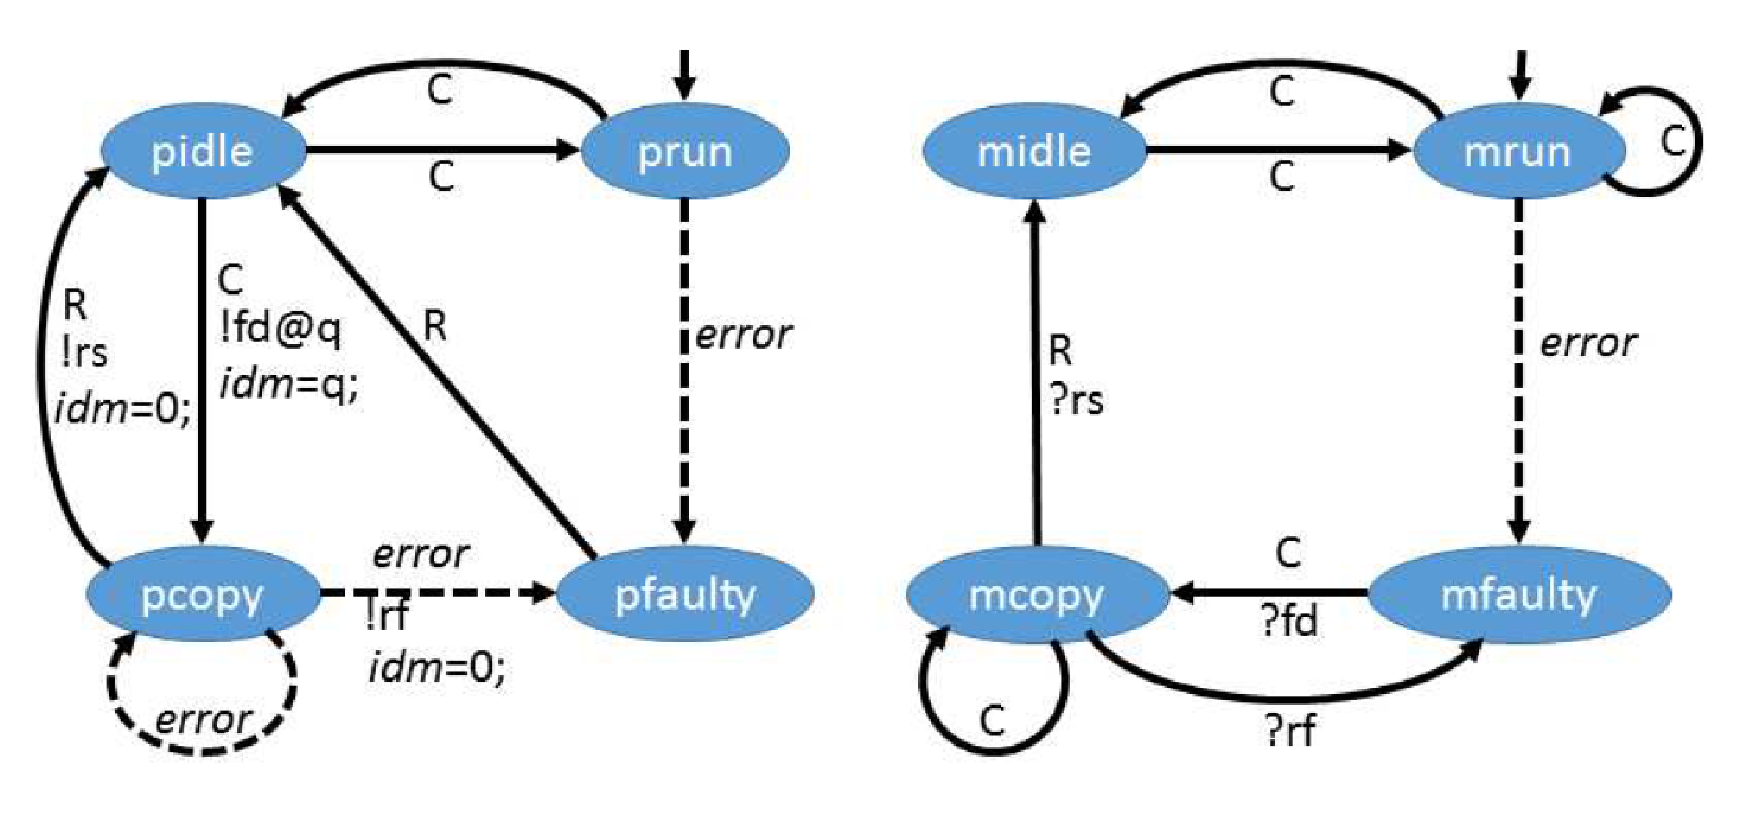
\epsfig{file=avi.eps,width=140mm} 
%\caption{CEFSM templates of $n$ processors and $m$ memory copies}
%\label{fig.pm}
%\end{center} 
%\end{figure*}
The CEFSM model has $n$ processors and $m$ memory modules. 
Figures~\ref{fig.pm}(a) and (b) are 
for the abstraction of processors and memory copies, respectively.  
The ovals represent local states of a processor or a 
memory module, while the arrows represent transitions. 
The transitions of a CEFSM are labeled with `$\emerr$', 
`C' (for Control), or `R' (for recovery).  

We also use synchronizers to bind process transitions. 
For example, when a memory module moves into a faulty state, 
an idle processor may issue an {\tt fd} (error-detected) event
and try to repair the module by copying memory contents from 
normal memory modules.  
Such error-detection is usually achieved with standard hardware.  
Note that the benchmarks are models that reflect the 
recovery mechanism, abstracting away the details of the original systems.  
A central issue in the design of this recovery mechanism is then 
the resilience level of the controlled systems.  
We need three synchronizers: 
\textit{fd} for error detection by a processor, 
\textit{rs} for recovery success, 
and \textit{rf} for recovery failure.  
The three synchronizers are used to bind a transition from a processor 
and another from a memory module into a synchronized transition.  
For example, a processor at state \textit{pidle} and 
a memory module at state 
\textit{mfaulty} may simultaneously enter their 
\textit{pcopy} and \textit{mcopy} states respectively
through synchronizers $!$\textit{fd} (for sending the synchronizer) 
and $?$\textit{fd} (for receiving). 
We also conveniently use a variable $q$ in this synchronized 
transition to capture the identifier of the memory module receiving 
the synchronizer.  
A transition without synchronization labels is considered a trivial 
synchronized transition.  
The transition system of the CEFSM operates with interleaving semantics 
at the abstraction level of the synchronized transitions. 

For counter abstraction, we need four global variables \textit{crp}, \textit{cfp}, 
\textit{crm}, and \textit{cfm} respectively 
to keep track of the numbers of running processors, faulty processors, 
running memory modules, and faulty memory modules. 
We also need a local variable \textit{idm} for each processor to record 
the faulty memory module identifier that the processor is 
responsible for recovery. 
We label the controllable, error, and recovery 
transitions respectively with `C', `$\emerr$', and `R'. 
We also label each transition with synchronizers and actions.  
At any moment, the processors and the memory modules 
may enter their running states, execute a task, and generate 
the outcome. 
A processor starts its execution from state \textit{prun} while 
a memory module starts from state \textit{mrun}. 


\subsection*{Step 2: building the product automata}
The product automata is a Kripke structure whose 
states are of is a vector $[p_1,\ldots,p_n,i_1,\ldots,i_n,s_1,\ldots,s_m]$ 
of $2n+m$ elements.  
For all $k$, $p_k$ and $i_k$ respectively represent the 
current location and the current \textit{idm} value of processor $k$ while 
$s_k$ represents the current location of memory module $k$.  
Then interleaving semantics that each time only a global transition 
(a single local process transition without synchronizers 
or two local process transition bound by a synchronizer) is executed 
is adopted to determine the transition relation from one state to another. 
Such techniques are standard in model construction.  
REDLIB can help in this regard by constructing the Kripke structure in 
an on-the-fly style to avoid the construction of those states not reachable 
from the initial state. 

\subsection*{Step 3: the labeling of the move vectors} 
After the second step, we have the game structure ready except for the 
move vectors on the transitions. 
We use $E_1=\{C,R,\mbox{\em nop}\}$, where {\em nop} represents ``no operation,"
and $E_2=\{\emnerr,\emerr\}$.  
Then we use the following three rules to label move vectors. 
\begin{list1} 
\item Every global transition with one component local process transition labeled 
	with $\emerr$ is labed with move vector $[\mbox{\em nop},\emerr\}$.  
\item Every global transition with a component local process transition labeled 
	with $R$ 	
	is labeled with move vector $[R,\emnerr]$.  
\item All other global transitions are labeled with move vector $[C,\emnerr]$.  
\end{list1} 


\subsection*{Counter abstraction of the example} 
We also use the CEFSM in figure~\ref{fig.pm} to explain counter abstraction. 
We need eight counter variables: 
{\em pr}, 
{\em pi}, 
{\em pc}, 
{\em pf}, 
{\em mr}, 
{\em mi}, 
{\em mc}, and 
{\em mf} to respectively record the 
number of processes in location prun, pidle, pcopy, pfaulty, mrun, midle, mcopy, and mfaulty
in a state.  
Then the counter abstraction of the CEFSM is in Figure~\ref{fig.pmC}.  
%\begin{figure*}[t] 
%\begin{center} 
%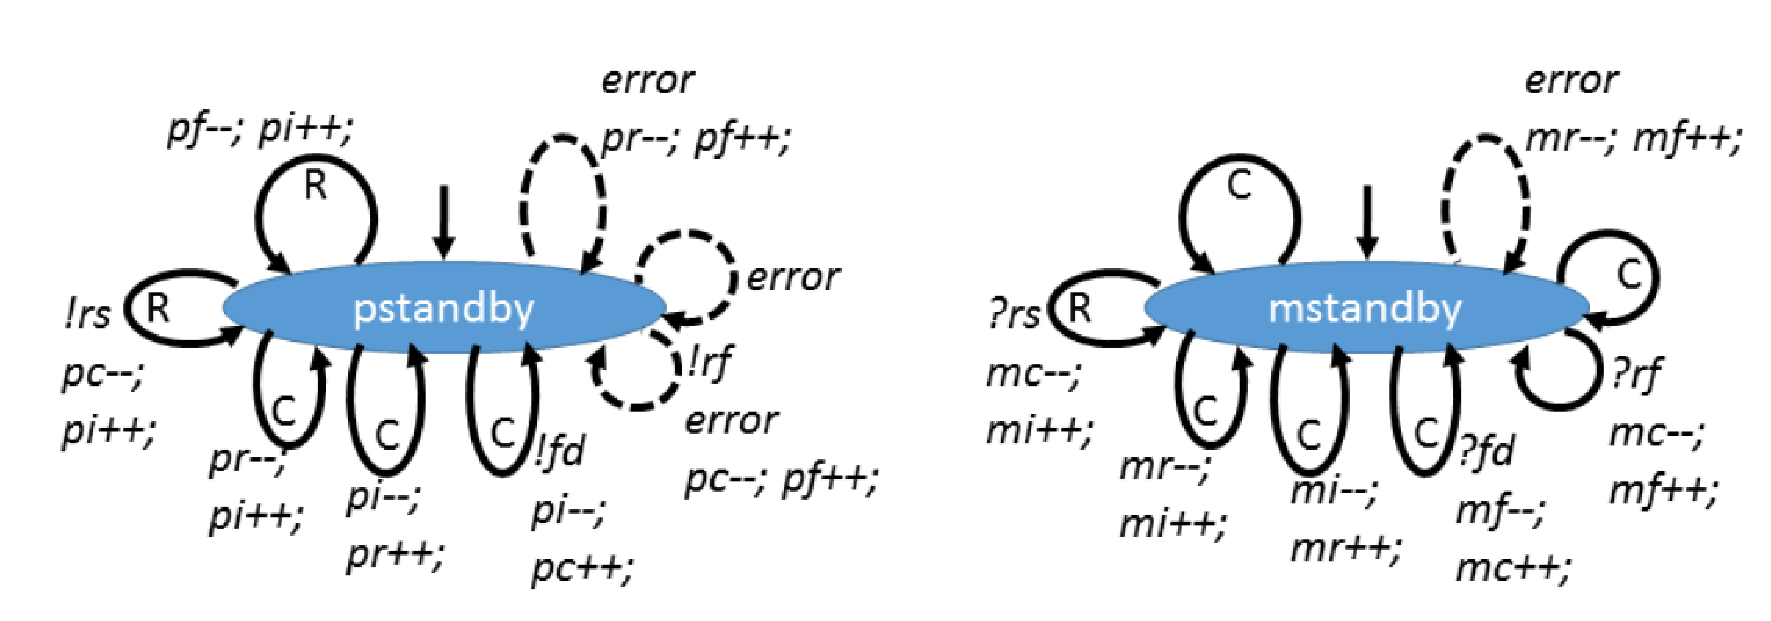
\epsfig{file=aviC.eps,width=140mm} 
%\caption{Counter abstraction of the CEFSM templates of $n$ processors and $m$ memory copies}
%\label{fig.pmC}
%\end{center} 
%\end{figure*}
The initial state are specified with constraint: 
$\mbox{\em pr}=n
\wedge \mbox{\em pi}=0
\wedge \mbox{\em pc}=0
\wedge \mbox{\em pf}=0
\wedge \mbox{\em mr}=m
\wedge \mbox{\em mi}=0
\wedge \mbox{\em mc}=0
\wedge \mbox{\em mf}=0$
on the counters.  
The state in the product automata must satisfy the following constraints: 
$\mbox{\em pr}+\mbox{\em pi}+\mbox{\em pc}+\mbox{\em pf}=n
\wedge \mbox{\em mr}+\mbox{\em mi}+\mbox{\em mc}+\mbox{\em mf}=m$.  
As can be seen, we do not care which processor is in the idle mode, 
in the running mode, etc., in this abstraction. 
Similarly, we do not care which memory module is in the idle mode, in the running mode, and etc. 
The local state transition only keeps tracks of the number of processors in each mode and 
the number of memory modules in each mode. 
We also do not care which processor is in charge of the recovery of which memory module.  
Such an abstraction can be done automatically.  

The labeling of the move vectors on the transitions in the Kripke structure (product automaton)
follows the same rules for the product automaton from the CEFSM in Figure~\ref{fig.pm}.  




\subsection*{Analysis of the game structure} 
The majority outcome of the processors and memory copies 
is used as the outcome of the system.  
A processor may enter the faulty state.  
A memory module may also enter the faulty state. 
Processors may control to recover themselves or a faulty memory module 
by copying the contents of a functioning memory module to 
the faulty one.  
At any moment, we want to make sure that we can always recover 
to a global condition with the following two restrictions. 
\begin{itemize} 
\item There are at least two more processors in \label{reply2.2more} 
	the running mode than the processors in the faulty mode.  
\item There are at least two more memory copies in 
	the running mode than memory copies in the faulty mode. 
\end{itemize} 
Together, the failure condition is 
$\textit{crp}-\textit{cfp}<2\vee\textit{crm}-\textit{cfm}<2$.  
That is, all states in the transition system satisfying 
$\textit{crp}-\textit{cfp}<2\vee\textit{crm}-\textit{cfm}<2$ 
are in set $F$.  

Tool implementation and the benchmarks used in the experiment 
can all be found in our Sourceforge REDLIB project at 
\verb+https://github.com/yyergg/Resil+.
\subsection{Performance data}
We report the performance data 
in Table~\ref{tab.perf} for the resilience algorithms 
described in Section~\ref{subsec.bench} 
against the parameterized benchmarks in the above with various 
parameters.  
The second column shows the concurrency sizes.  
The third column shows the values of $k$ for the rows.  
The fourth and fifth columns show the sizes of the concurrent game structures.  
The sixth and seventh columns show the time and spaces used to calculate 
sfrch$_k()$.  
Similarly, the eighth and ninth columns show the time and spaces for calculating 
the res$_k()$.  

The benchmark in Figure~\ref{fig.pm} does not have nodes in 
$\safe_2(G)$ and $\res_2(G)$.  
So we changed the benchmark to see how we check our implementation 
with $k>1$.  
The change is that the recovery transition from state \textit{pcopy} to 
\textit{pidle}
of processors are relabeled as controllable. 
This change significantly limits the ability of the system errors 
to derail the system.  
\begin{table*}[t] 
\caption{Performance data for resilience calculation \hspace{21mm} s: seconds; M: megabytes} 
\label{tab.perf} 
\begin{center} 
\resizebox{\columnwidth}{!}{
\begin{tabular}{l|c|c|c|c||c|c||c|c} \hline 
benchmarks & concurrency & $k$ & \multicolumn{2}{c||}{game sizes} 
& \multicolumn{2}{c||}{sfrch$_k$}  
			& \multicolumn{2}{c}{res$_k$} \\\cline{4-9} 
	 & 	& & \#nodes & \#edges & time  & memory   & time & memory  \\
\hline \hline 
avionics & 2 processors \& 2 memory modules 
     & 2 & 118 & 750 
     & 0.62s & 114M & 0.85s & 116M \\ \cline{2-9} 
     & 2 processors \& 3 memory modules 
     & 2 & 414 & 3252
     & 0.94s & 139M & 1.10s & 153M \\ \cline{2-9} 
     & 3 processors \& 3 memory modules 
     & 3 & 1540 & 15090 
     & 4.67s & 225M & 8.38s & 267M \\ \cline{2-9} 
     & 3 processors \& 4 memory mdules
     & 3 & 5601 & 63889 
     & 42.86s & 815M & 155s & 846M \\ \hline  
avionics & 6 processors \& 6 memory modules 
	 & 2 & 1372 & 6594 
	 & 2.89s & 129M & 3.54s & 516M \\ \cline{2-9} 
(counter	 & 7 processors \& 7 memory modules 
	 & 3 & 2304 & 11396 
	 & 10.7s & 216M & 23.4s & 808M \\ \cline{2-9}
abstraction)	 & 8 processors \& 8 memory modules 
	 & 3 & 3645 & 18432 
	 & 43.8s & 1009M & 135s & 2430M \\ \hline 
voting	 & 1 client \& 20 replicas 
	 & 9 & 9922 & 23551 & 7.01s & 260M & 36.7s & 297M \\ \cline{2-9} 
	 & 1 client \& 26 replicas 
	 & 12 & 20776 & 49882 & 19.9s & 474M & 79.6s & 611M \\ \hline 
simple	 & 1 client \& 150 replicas 
	 & 74 & 458 & 1056 & 0.71s & 159M & 31.7s & 219M \\ \cline{2-9} 
voting	 & 1 client \& 200 replicas 
	 & 99 & 608 & 1406 & 1.06s & 161M & 162s & 337M \\ \cline{2-9} 
	 & 1 client \& 250 replicas 
	 & 124 & 758 & 1756 & 1.36s & 163M & 307s & 499M \\ \hline 
PBFT 	 & 1 client \& 6 replicas 
	 & 2 & 577 & 897 & 0.34s & 72M & 1.05s & 193M \\ \cline{2-9} 
	 & 1 client \& 9 replicas 
	 & 4 & 2817 & 4609 & 13.3s & 564M & 58.5s & 1657M \\ \hline 
clock	 & 1 client \& 15 servers  
	 & 7 & 16384 & 229376 & 45.1s & 3075M & 62.4s & 3264M  \\ \cline{2-9} 
sync	 & 1 client \& 17 severs  
	 & 8 & 65536 & 1070421 & 870s & 14725M & 915s & 15433M  \\ \hline 
\end{tabular}
}
\end{center}
\vspace*{-5mm}
\end{table*}
For the avionics system, %the $k$ value
the resilience level $k$ is set to 
one less than half the %value
number of processors.  
For the voting and simple voting benchmarks, 
the value of $k$ is set to one less than half the number of 
replicas (voters). 
For the PBFT and clock synchronization algorithm, we choose 
$k$ to be one less than one third of the number of replicas. 

The performance data has been collected with a Virtual Machine (VM) 
running opensuse 11.4 x86 
on Intel i7 2600k 3.8GHz CPU 
with 4 cores and 8G memory. 
The VM only uses one core and 4G memory.  

The time and space used to calculate resilience is a little bit more 
than that to check for $\safe$.  
The reason is that $\safe_k$ is a pre-requisite for calculating $\res_k$.  
In our experiment, $\safe_k$ is usually 
very close to $\res_k$ and does not require much extra time in 
calculating $\res_k$ out of $\safe_k$.  

The experiments show that our techniques 
scale to realistic levels of redundancy.  
For fault-tolerant hardware, usually the numbers of replicas are small, 
for example, less than 10 replicas. 
Thus our techniques seem very promising for the 
verification and synthesis\label{reply2.verification.hardware} of hardware fault-tolerance.  

On the other hand, 
nowadays, software fault-tolerance through networked computers can 
create huge numbers of replicas.  
Our experiment shows that counter abstraction can be a useful 
techniques for the modeling and verification of software resilience.  
Specifically, for the avionics benchmark, 
we can verify models of much higher concurrency and complexity with 
counter abstraction than without. 
% As can be seen, our techniques can really prove the % safety and 
% resilience of pretty large concurrency sizes.  
\section{Related works}
We have applied game-based technqiues~\cite{Church63,PR89a,Rabin69} \label{reply1.related.work.1st.para} 
for synthesizing a control mechanism with maximal resilience to software errors.  
The synthesis of control strategies is essential in solving games with temporal and $\omega$-regular objectives.  
For these more complex objective, synthesis goes back to Church's solvability problem~\cite{Church63} and 
inspired Rabin's work on finite automata over infinite 
structures~\cite{Rabin69} and 
B\"uchi and Landweber's works on finite games 
of infinite duration~\cite{Buchi62,BL69}. 
A righ body of literature on synthesis
has since been developed \cite{AAE04,EKA08,GR09,KV00,PR89b,Rushby92,SF06}.

Traditionally, fault tolerance refers to various basic fault models~\cite{AAE04}, 
such as a limited number of errors \cite{JRT04}.
These traditional fault models are subsumed 
by more general synthesis or control objectives 
\cite{AMP95,AAE04,Thomas94};\label{reply2.RW} 
as simple objectives with practical relevance, 
they have triggered the development of specialized tools~\cite{EKA08,GR09}.

Dijkstra's self-stabilization criterion~\cite{AG93,Dijkstra86} suggests to build systems that eventually recover
to a `good state', from where the program commences normally.
Instead of {\em constructing} a system to satisfy such a goal, one
might want to apply control theory to {\em restrict} the execution of
an existing system to achieve an additional goal.
Our control objective is a recovery mechanism for up to $k$ errors.
After recovery, the system has to tolerate up to $k$ errors again, and so forth.
In this work, 
we suggest a mechanism to synthesize a recovery mechanism for a given fault model and recovery primitives.


In \cite{DHLN10}, an interesting notion of robustness based on Hamming 
and Lewenstein distance related to the number of past states is defined. 
It establishes a connection between these distances with a notion of 
synchronization that characterizes the ability of the system to reset for 
combinatorial systems.
In \cite{BGHJ09}, `ratio games' are discussed, where the objective is 
to minimize the ratio between failures induced by the environment and system errors caused by them.


Besides using our simple game model that neither refer directly to time, nor to probabilities, one can also consider models that make these aspects explicit.
Their analysis is far more complex (with \cite{FRSZ11} offering the best complexity bounds), and so are the resulting strategies.
If we, for example, return to the example of airplanes with an operation time of 20 hours referred to in Table \ref{tab.mtbf}, then an optimal timed model would take the remaining operation time into account.
When the remaining time is two minutes, the balance between being resilient against waves of two errors and being resilient against 5 errors looks very different, and the optimal control would change over time rather than being static.
Another implication of more complex models would be that the error model would have to be more detailed.
Even if one assumes that a simple concept like safe states persists, it depends on the fineties of such a model if a two step path back to it where an error after step one leads to system failure is preferable over a much longer path, say through 10,000 intermediate states, where one error can be tolerated during recovery.

We believe that the independence from such details is an advantage of our technique, partly because it is simpler and cheaper, and partly because the further advantages one can obtain from more detailed error models rely heavily on very knowledge of (or, realistically, on very detailde assumptions on) how errors are distributed.
\label{reply1.prob.more.complex}  

%\paragraph{\bf Organization of the article.}
%We suggest a two layered approach:
%in a first layer, we simplify a complex system to the aspects relevant for its control.
%This abstraction layer of our approach reduces life size examples to small abstractions 
% (Example~\ref{exmp.avi}).
%%
%In Section~\ref{sec:kresil}, we provide computationally cheap algorithms to synthesize a strategy for controlling the system to allow for up to $k$ dense failures.
%Such a strategy restricts the choices of the system to achieve resilience towards $k$ failures.
%Failure to construct such a strategy means that the system is not $k$-resilient.
%% Through the abstraction used, a
%Achieving the fault tolerance goal by controlling the system through the calculated strategy, provides a guarantee that the executions of the controlled system are included in the original executions of the system.
%This, in turn, guarantees that {\em all} (linear) temporal properties of the system are preserved.
%%
%We describe our implementation and discuss experimental results in Section~\ref{sec.imp.exp}.

%% >>> changes start 


In \cite{EhlersT14,BloemEJK14} the resilience model we have introduced \cite{HPSW/12/rapidRecovery} has been applied for synthesising robust control in an assume-guaranee setting to produce robustness against occasional noncompliance of the environment with the assumptions of its behavior.

%% <<< changes end

\section{Conclusion \label{sec.conc}}
We have introduced an approach for the development of a control of safety critical
systems that maximizes the number of \emph{dense} errors the system can tolerate.
Our techniques are inspired by the problem of controlling systems with redundancy:
in order to deflect the effect of individual errors, safety critical systems are often equipped with multiple copies of various components.
If one or more components fail, such systems can still work properly as long as the correct behavior can be identified.
 
This has inspired the two-phase formulation of the safety resilience problems in this article.
In the first phase, we identify a $k$-resilient region\label{reply2.need.identify},  
while\label{reply2.layer} we develop a control strategy for recovery in the second phase.  
After an error, the controller can recover to the $k$-resilient region without encountering a system failure, unless the error is part of a group of more than $k$ errors that happen in close succession.
Such a recovering strategy is memoryless.
Being memoryless on a small abstraction in particular implies that the recovery is fast.

The system can, once recovered, tolerate and recover from $k$ further dense errors, and so forth.
Consequently, our control strategy allows for recovery from an arbitrary
number of errors, provided that the number of dense errors is restricted.
This is the best guarantee we can hope for: our technique guarantees to find the optimal parameter $k$.
%
This parameter is bound to be small (smaller than the number of redundant components).
Optimizing it is computationally inexpensive, but provides strong guarantees: the likelihood of having more than $k$ errors appear in short succession after an error occurred are, for independent errors, exponential in $k$. As errors are few and far between, each level of resilience gained reduces the likelihood of 
system-level failures significantly.
\chapter{Basic Strategy-interaction Logic}
\label{c:bsil}

\section{Running Example}
We use a banking example to explain the idea of this work. 
Suppose that a bank want to provide the following services. 
\begin{list1}
\item No client is allowed to check other's password
\item Depositing to an account by a client from the root screen. 
\item Transferring money from an account in the bank to an account in another bank, also from the root screen.
\item There is only one bank system, which means the strategy of the bank system which fulfilled above specification should be identical.
\end{list1} 
As we can see, the deposit service involves the interaction between a client and the bank while the transfer service involves at least three parties: a client, the bank, and a partner bank.
Also in the meantime, the bank wants to forbid any client and partner from checking sensitive information of other clients, .e.g., checking the password of another client.  

\subsection{Trying to Write Down a Correct Formal Specification}
To develop the services, the bank manager in charge of the project need specify the services and make sure that the specification is not erroneous.
If they turn to the literature, the bank manager may choose ATL or its extensions, e.g., fair ATL, ATL*, AMC, GL, etc., to specify the services. 
The choice is plausible at first glance since ATL and fair ATL both have a polynomial time model-checking algorithm and could support the verification of the services.
So the manager could easily specify the services with the following formula. 
\begin{center} \hfill 
$\langle 1\rangle\left(\begin{array}{cl}
		& \pfrr\neg \mbox{\sl checkOthersPassword}\\
\wedge 	& \langle 2\rangle \pevt \mbox{\sl depositDone} \\
\wedge  & \langle 2, 3\rangle\pevt\mbox{\sl transferDone} 
\end{array}\right)$
\hfill (C) 
\end{center}   
Here we use agent index 1 for the bank, 2 for the client, and 3 for the partner bank.
But on a second look, we can see that that this specification is too restrictive.  
Subformula $\langle 2\rangle\pevt \mbox{\sl depositDone}$ says that the client can force a deposit transaction no matter how the banking system responds. 
In practice, there are many factors beyond the control of the client for the success of a transaction.  
For example, when the banking system is in maintenance or out of order, then the transaction may fail.  

After realizing the problem with formula (C), the manager decides to rewrite the specification as follows.
\begin{center} \hfill 
$\begin{array}{cl}
		& \langle 1\rangle \pfrr\neg \mbox{\sl checkOthersPassword}\\
\wedge 	& \langle 1,2\rangle \pevt \mbox{\sl depositDone} \\
\wedge  & \langle 1,2, 3\rangle\pevt\mbox{\sl transferDone} 
\end{array}$
\hfill (D) 
\end{center}   
This specification fixes the issue observed in formula (C) since now $\langle 1,2\rangle\pevt\mbox{\sl depositDone}$ says with the collaboration of the banking system, the client can finish a deposit transaction.  
However, there is a subtle issue which nullifies the formula.  
In the collaboration between the banking system and the client for property $\langle 1,2\rangle\pevt\mbox{\sl depositDone}$, the banking system is no longer required to maintain property $\pfrr\neg \mbox{\sl checkOthersPassword}$ since according to the semantics of ATL, the specification does not require the banking system to use the same strategy to enforce both $\langle 1\rangle \pfrr\neg \mbox{\sl checkOthersPassword}$ and $\langle 1,2\rangle \pevt \mbox{\sl depositDone}$.  
The same issue also appears in $\langle 1,2,3\rangle\pevt\mbox{\sl transferDone}$.  
That is, the banking system's strategy in enforcing $\langle 1,2,3\rangle\pevt\mbox{\sl transferDone}$ is not required to be the same one in enforcing $\langle 1\rangle \pfrr\neg \mbox{\sl checkOthersPassword}$.
Thus, the bank cannot sue their contractors for developing the service system if the systems leaks clients' passwords in transferring funds.

\subsection{Resorting to General Strategy Logics for a Correct Specification}
After several trials, the manager eventually finds out that the specification cannot be expressed in ATL, ATL*, GL, and AMC \cite{AHK02}.
Then the manager turns to strategy logics \cite{CHP10,MMV10} in the literature and finds out that the specification can be expressed as follows. 
\begin{center} \hfill 
$\langle x\rangle \langle y\rangle\langle z\rangle \langle w\rangle \left(\begin{array}{cl}
		& (1,x)\pfrr\neg \mbox{\sl checkOthersPassword}\\
\wedge 	& (1,x)(2,y)\pevt \mbox{\sl depositDone} \\
\wedge  & (1,x)(2,z)(3,w)\pevt\mbox{\sl transferDone} 
\end{array}\right)$
\hfill (E) 
\end{center}   

This formula declares four existentially quantified strategies: $x,y,z$, and $w$, and says the following. 

\begin{list1} 
\item On using strategy $x$, the banking system can enforce $\pfrr\neg \mbox{\sl checkOthersPassword}$.  
\item On using strategy $x$ and $y$ respectively, the banking system and a client can 
  finish the deposit transaction.  
\item On using strategy $x$, $z$, and $w$ respectively, the banking system, the client, and 
  a partner bank can also finish a fund transfer transaction.  
\end{list1} 

The manager is happy with the elegant specification and wants to verify the specification on the model of the development delivery.
Then he finds out that there is no tractable algorithm and working tools for checking this specification or synthesize the strategies.
In fact, the complexity reported in the literature is at best doubly exponential \cite{CHP10,MMV10}. 
So the manager finds himself in the dilemma between expressiveness and verification efficiency.  

But when the manager bangs his head to the theoretical challenges, he soon realizes that strategy logics offer more expressiveness than he expects.
For example, he could write down the following formula.
\begin{center} 
\hfill 
$\langle x\rangle \langle y\rangle[ z] \langle w\rangle \left(\begin{array}{cl}
		& (1,x)\pfrr\neg \mbox{\sl checkOthersPassword}\\
\wedge 	& (1,x)\pfrr (2,y)\pevt \mbox{\sl depositDone} \\
\wedge  & (1,x)\pfrr (2,z)(3,w)\pevt\mbox{\sl transferDone} 
\end{array}\right)$
\hfill (F) 
\end{center}  
Here $[z]$ universally quantifies a strategy named $z$.  
Thus subformula $(1,x)(2,z)(3,w)\pevt\mbox{\sl transferDone}$ in fact says that the banking system has a strategy $x$ such that for all strategies $z$ of the client, the partner bank have a strategy $w$ to help enforcing $\pevt\mbox{\sl transferDone}$.
Considering that a strategy is an action decision function on the history, this in fact means that strategy $w$ is clairvoyant and contradicts the implementation assumption of all practical banking systems.  
Indeed the huge verification complexity of strategy logics can be attributed to such free-style binding operations of strategy names to agents.  
Thus, the manager asks himself whether there is a subclass of strategy logics that allows for elegant expressions of natural and practical specifications while supporting verification with less complexity.
Similar examples in fact can appear in different projects with services that rely on collaboration of multiple agents.

\subsection{BSIL: New Strategy Modalities Expressive Enough for the Specification}
In fact, in conceivable applications, the developers cannot implement and are not interested at clairvoyant strategies.  
In other words, for practical specifications, it is likely that existential SIQs are expressive enough.
In BSIL, formula (E) can be rewritten as follows.
\begin{center} \hfill 
$\langle 1\rangle \left(\begin{array}{cl}
		& \pfrr \neg \mbox{\sl checkOthersPassword}\\
\wedge 	& \langle +2\rangle\pevt \mbox{\sl depositDone} \\
\wedge  & \langle+2,3\rangle\pevt\mbox{\sl transferDone} 
\end{array}\right)$
\hfill (G) 
\end{center}
This formula says that the banking system has a strategy that at any instant, the system can ensure that no password is leaked, the system allows a client to finish a deposit transaction, and the system allows a client to transfer funds from or to a partner bank.

\subsection{Symbolic Strategy Names and Path Obligations}
But to verify such a BSIL property, we need new techniques to check that along plays, the same decision is made for the same strategy.  
Consider the model of the banking system in figure~\ref{fig.model.bank}.  
\begin{figure*}[t] 
\begin{center} 
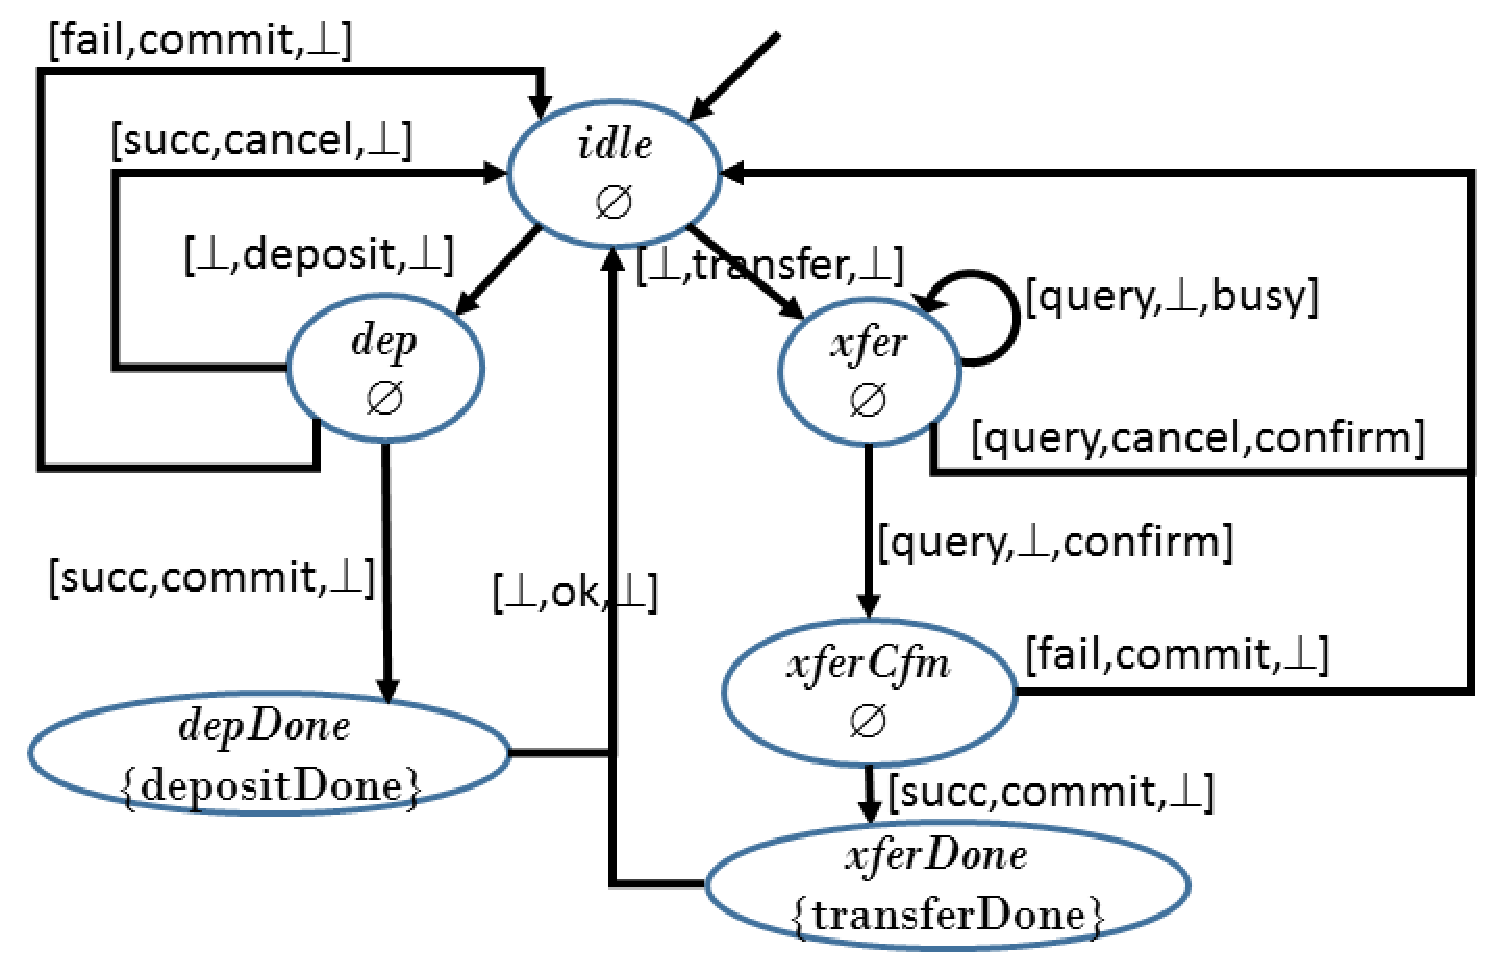
\epsfig{file=bank.eps,width=120mm} 
\caption{Game graph of a banking system} 
\label{fig.model.bank}
\end{center} 
\end{figure*} 
We need to find strategies of the agents to fulfill 
$\pfrr \neg \mbox{\sl checkOthersPassword}$, 
$\pevt \mbox{\sl depositDone}$, and 
$\pevt\mbox{\sl transferDone}$.  
To assist in our explanation of our verification algorithms, 
we use symbolic strategy names $x,y,z,w$ and the binding notations in formula (F).  
In fact, formula (G) is exactly the same as formula (E).  
Thus by interpreting all symbolic strategy names as existential quantified, 
formula (G) can be rewritten as follows.  
\begin{center} \hfill
$
\begin{array}{cl}
((1,x) \pfrr \neg \mbox{\sl checkOthersPassword}) \\
\wedge ((1,x)(2,y)\pevt \mbox{\sl depositDone}) \\
\wedge ((1,x)(2,z)(3,w)\pevt\mbox{\sl transferDone})
\end{array}
$
\hfill (H)
\end{center}   
Note that since we only allow explicit existential strategy quantification, 
the number of strategy bindings are exactly determined by the number and sizes of SQs and SIQs 
in the formula.  


If we label $(1,x) \pfrr \neg \mbox{\sl checkOthersPassword}$, $(1,x)(2,y)\pevt \mbox{\sl depositDone}$, and $(1,x)(2,z)$ $(3,w)\pevt\mbox{\sl transferDone}$ on nodes of a computation tree in a labelling procedure, then the symbolic names precisely reflect the the constraints on the decisions along plays. 
For example, suppose that both $(1,x) \pfrr \neg \mbox{\sl checkOthersPassword}$ and $(1,x)(2,y)\pevt \mbox{\sl depositDone}$ are labelled on a state of location {\em dep}. 
This state has three successor states: for convenience 
C1 of location {\em idle} via $[\mbox{\rm fail},\mbox{\rm commit},\perp]$, 
C2 of location {\em idle} via $[\mbox{\rm succ}, \mbox{\rm cancel}, \perp]$, and 
C3 of location {\em depDone} via $[\mbox{\rm succ}, \mbox{\rm commit}, \perp]$.  
If strategy $x$ chooses action succ, then obligation $(1,x) \pfrr \neg \mbox{\sl checkOthersPassword}$ will be passed down to C2 and C3.  
In this situation, whether obligation $(1,x)(2,y)\pevt \mbox{\sl depositDone}$ is labeled on C2 or C3 relies on the action decision of strategy $y$.  
But the constraint on strategy decision is that if $(1,x)(2,y)\pevt \mbox{\sl depositDone}$ is labeled on C2, then $(1,x) \pfrr \neg \mbox{\sl checkOthersPassword}$ must also be labeled on C2; and if  $(1,x)(2,y)\pevt \mbox{\sl depositDone}$ is labeled on C3, then $(1,x) \pfrr$ $\neg \mbox{\sl checkOthersPassword}$ must also be labeled on C3.  
The reason is that the path obligations are enforced by the same strategy of the bank.  

\subsection{Passing Down the Path Obligations While Observing the Restrictions Among S-Profiles}
The above observation points out how to judge whether a passing-down scheme of path obligations from a parent state to its child states are consistent with the strategy quantifications.  
For example, suppose that we have the following characteristics of the strategy profile $(1,x)(2,y)(2,z)(3,w)$.
\begin{list1} 
\item Strategy $x$ of the banking system never issues action fail. 
\item Strategy $y$ and $z$ never cancel transactions for its client. 
\item Strategy $w$ never shows busy message for the partner bank. 
\end{list1} 
Then the verification problem of strategy interaction can be visualized as finding strategies $x,y,z$, and $w$ that selecting paths in a computation tree to satisfy three path obligations: 
$\pfrr \neg \mbox{\sl checkOthersPassword}$, 
$\pevt \mbox{\sl depositDone}$, and $\pevt\mbox{\sl transferDone}$.  
Figure~\ref{fig.ctree} shows part of a computation tree when strategy $x$ for the banking system is fixed with the following restriction. 
\begin{figure*}[t] 
\begin{center} 
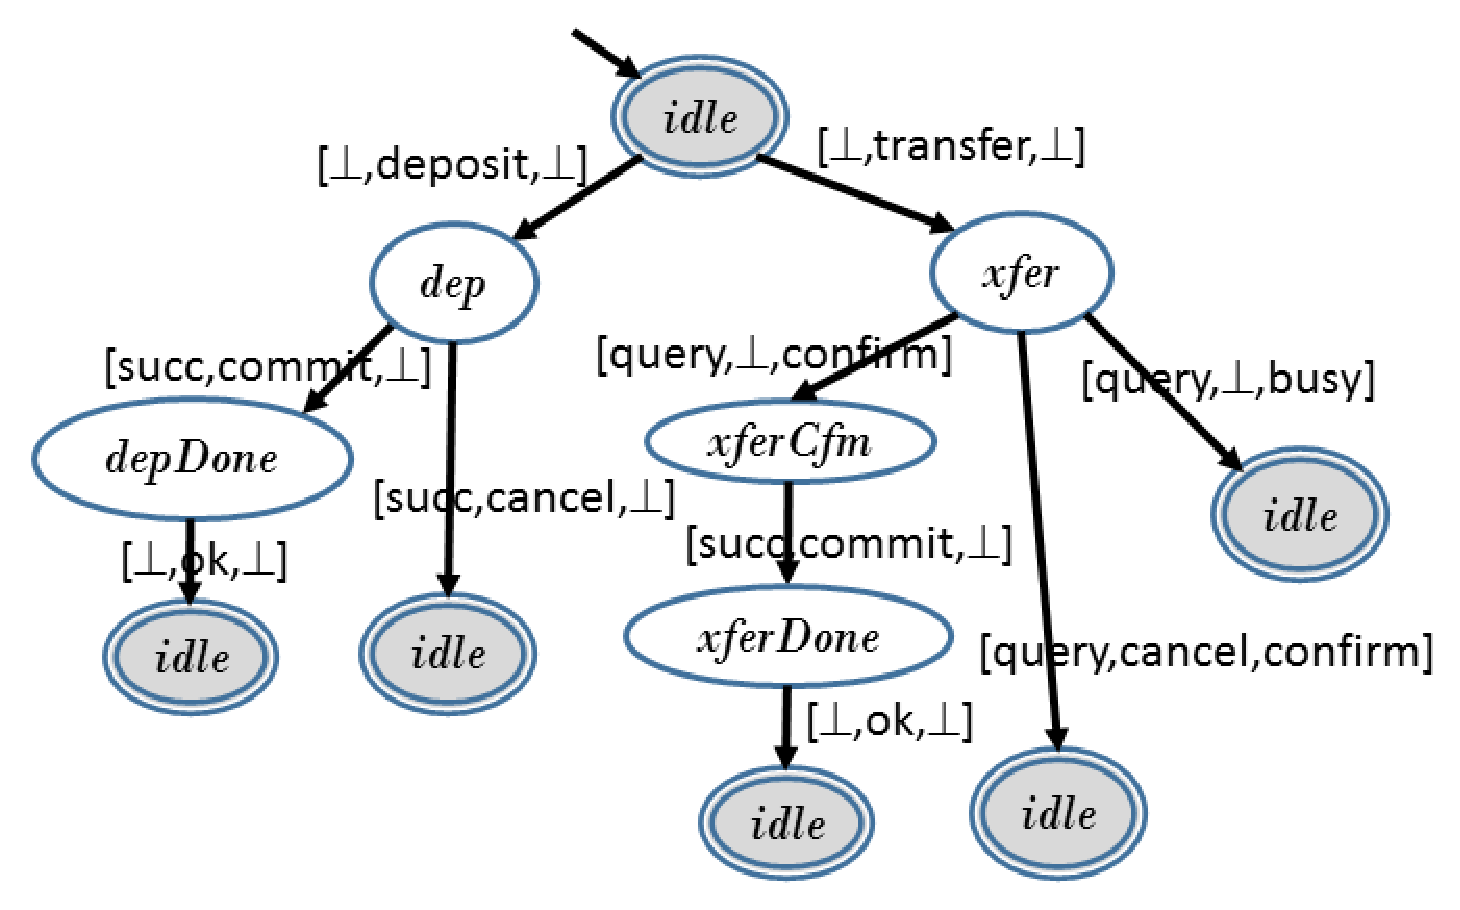
\epsfig{file=ctree.eps,width=120mm} 
\caption{Part of the computation tree of the banking system} 
\label{fig.ctree}
\end{center} 
\end{figure*} 
\begin{list1} 
\item At location {\em idle}, {\em depDone}, and {\em xferDone}, always issue action $\perp$.  
\item At location {\em dep} and {\em xferCfm}, only issue action {\sf succ}.  
\end{list1}
The leaves of the tree all end at location {\em idle} at which the same tree structure can be replicated.
We can start synthesizing strategy $y,z$, and $w$ in the context of this strategy $x$ which, for convenience of explanation, is memoryless (or positional). 

As we have suggested, we can label the path obligations on the nodes of the computation tree and examine whether a strategy profile can fulfill all the path obligations.
In the literature, we can name the nodes by their branching paths.
For example, the root is named $\varepsilon$ which is the empty string. 
Then the node at location {\em xferDone} is named '100' and 
the rightmost {\em idle} node is named '12.' 
We begin by label node `$\varepsilon$ with the three path obligations: 
$(1,x) \pfrr \neg \mbox{\sl checkOthersPassword}$, 
$(1,x)(2,y)\pevt \mbox{\sl depositDone}$, and $(1,x)(2,z)(3,w)$ $\pevt\mbox{\sl transferDone}$.  
Then we can pass the path obligations to the children in the following way. 
\begin{list1}
\item We must pass $(1,x) \pfrr \neg \mbox{\sl checkOthersPassword}$ to 
  both child '0' and '1' of the root since the two children 
  are both selected by action $\perp$ of the banking system. 
\item We can pass $(1,x)(2,y)\pevt \mbox{\sl depositDone}$ 
	and $(1,x)(2,z)(3,w)\pevt\mbox{\sl transferDone}$ respectively to 
	child '0' and '1' of the root since 
	the two children are selected with the same strategy $x$ of the banking system 
	and different strategies ($y$ and $z$) of the client.  
\end{list1} 
Note that we can check whether the passing down of the path obligation is consistent with the strategy quantifications in the input formula (G) just by checking the labelling of path obligations with strategy name bindings since all consistency information are maintained there.

Similarly, from node '0', strategy $x$ and $y$ can together choose to pass 
$(1,x)(2,y)\pevt$ $\mbox{\sl depositDone}$ to node '00' while strategy $x$ must unilaterally pass 
$(1,x) \pfrr \neg$ $\mbox{\sl checkOthersPassword}$ 
to both '00' and '01.'  
Then at node '00,' $(1,x)(2,y)\pevt \mbox{\sl depositDone}$ is fulfilled 
eventually and no longer need be passed down.  
The passing down of path obligations from node '1' and fulfillment of 
$(1,x)(2,z)(3,w)\pevt\mbox{\sl transferDone}$ can then be reasoned similarly.
 
\subsection{Finding Finite Satisfying Evidence for a Formula in a Computation Tree}
As we can see, the existence of the tree top in figure~\ref{fig.ctree} is sufficient for synthesizing strategy profile $(1,x)(2,y)(2,z)(3,w)$ to satisfy formula $(G)$.  
From this example, it is easy to see that the requirement for such a tree top.  
First, all eventual-formulas (or until-formulas) from the root SQ to the next level of SQs have to be fulfilled by the strategy profile.
Second, the leaves of the tree top do not contain any eventual-formula (or until-formula) labels.
Thus our PSPACE algorithm for model-checking BSIL formulas is actually a non-deterministic one that guess and check the consistency of the tree top and strategic actions at the nodes in the tree top.  

Then the final question regarding our algorithms is the terminating condition for searching the tree tops and strategy profiles.
Let us consider a tree node labelled with path obligations and how to (non-deterministically) explore for a tree top and a strategy profile.  
Note that the path obligations labelled on a child will be no more than those of its parent.  
In fact, the path obligations can stop being passed down in a path when it is fulfilled. 
Path obligations are simply passed down and not generated along the paths.  
As a result, along a path longer than the size of the game graph, either the number of path obligations decreases or two nodes, say $v$ and $v'$ 
(for convenience, we assume $v$ is an ancestor of $v'$), with identical location and labels must appear.
If the tree top is an evidence of existence of a strategy profile and the latter happens, then we can replace the the subtree rooted at $v$ with the one rooted at 
$v'$ and the result tree top is still an evidence.
This observation implies that we can focus on tree top such that along any path, no duplication of nodes with the same location and the same path obligation labels.  
This implies that we only have to explore tree tops of depth no greater than the size of the game graph times the number of temporal modalities in the given BSIL formula.


\section{BSIL}
\subsection{Syntax}
For concurrent game graph $\calg$ of $m$ agents, we have three types of formulas: {\em state formulas}, {\em tree formulas}, and {\em path formulas}.  
State formulas describe properties of states.  
Tree formulas describe interaction of strategies.  
Path formulas describe properties of plays.  
BSIL formulas are constructed with the following three syntax rules, 
respectively, for state formulas $\phi$, 
tree formulas $\tau$, and 
path formulas $\theta$.  
\begin{center}
$\begin{array}{rcl}
\phi    & ::= & p\;|\; \neg \phi_1 \;|\; \phi_1\vee \phi_2 
    \;|\; \langle  A\rangle \tau
    \;|\; \langle  A\rangle \theta
    \\
\tau  & ::= & \tau_1\vee \tau_2 \;|\; \tau_1\wedge \tau_2
    \;|\; \langle+ A\rangle \tau_1
    \;|\; \langle+ A\rangle\theta 
    \\
\theta  & ::= & \neg\theta_1 \;|\; \theta_1\vee \theta_2 
    \;|\; \nxt \phi_1
    \;|\; \phi_1\until \phi_2
\end{array}$
\end{center}
Here, $p$ is an atomic proposition in $P$ and
$A$ is an agency of $[1,m]$.
$\langle A\rangle$ is a {\em strategy quantifier} ({\em SQ}) and 
$\langle +A\rangle$ is a {\em strategy interaction quantifier} ({\em SIQ}).  
$\langle A\rangle\psi$ means that
there exists an S-profile for the agency $A$
that makes all plays satisfy $\psi$.
Formulas of the form $\langle+ B\rangle\psi_1$ must happen within an SQ.
Intuitively, they mean that there exists an S-profile of $B$
that collaborates with the strategies declared 
with ancestor formulas to make $\psi_1$ true. 
For convenience, we view SQs as special cases of SIQs. 
Also, for conciseness, we omit null SIQs $\langle+\rangle$.

State formulas $\phi$ are called {\em BSIL} {\em formulas}. 
From now on, we assume that we are always in the context of 
a given BSIL formula $\chi$.  
Note that we strictly require that strategy interaction cannot 
cross path modal operators.  
This restriction is important and allows us to analyze the interaction 
of strategies locally in a state and 
then enforce the interaction along all paths from this state.  

For convenience, we also use the common shorthands.
\begin{center} 
$
\true
\equiv p\vee(\neg p) 
\hspace*{10mm} 
\false
\equiv \neg\true 
\hspace*{10mm} 
\psi_1\Rightarrow \psi_2
\equiv (\neg \psi_1)\vee \psi_2$ \\
$\pevt \phi_1
\equiv \true\;\until \phi_1 
\hspace*{20mm} 
\pfrr \phi_1
\equiv \neg\pevt\neg\phi_1 
$
\end{center} 
The SQs and SIQs introduced above are 
all existential in that they are satisfied with one S-profile.  
Note that there is no universal SQs and SIQs in BSIL.  
This is purely for the complexity of the model-checking algorithm (and problem)
that we are going to present later.  
Thus BSIL can be used to specify the different ways of combining S-profiles 
to enforce system policy.  

For ease of notations, 
we may abbreviate 
$\langle \{a_1,\ldots,a_n\}\rangle$ and  
$\langle+ \{a_1,\ldots,a_n\}\rangle$ as 
$\langle a_1,\ldots,a_n\rangle$ and  
$\langle+a_1,\ldots,a_n\rangle$, respectively.
\subsection{semantics}
BSIL subformulas are interpreted with respect to S-profiles.  
A state or a tree formula $\phi$ is satisfied 
at a state $q$ with S-profile $\Sigma$, denoted $\calg,q\models_\Sigma\phi$, if,
and only if, the following inductive constraints are satisfied.
\begin{list1}
\item $\calg,q\models_\Sigma p$ iff $p\in \lambda(q)$.
\item For state formula $\phi_1$, 
    $\calg,q\models_\Sigma\neg\phi_1$ iff
    $\calg,q\models_\Sigma\phi_1$ is false.
\item For state or tree formulas $\psi_1$ and $\psi_2$, 
    $\calg,q\models_\Sigma\psi_1\wedge\psi_2$ iff
    $\calg,q\models_\Sigma\psi_1$
    and $\calg,q\models_\Sigma\psi_2$.
\item For state or tree formulas $\psi_1$ and $\psi_2$, 
    $\calg,q\models_\Sigma\psi_1\vee\psi_2$ iff
    either $\calg,q\models_\Sigma\psi_1$
    or $\calg,q\models_\Sigma\psi_2$.
\item $\calg,q\models_\Sigma\langle A\rangle\tau$
    iff there exists an S-profile $\Pi$ of $A$
    with $\calg,q\models_{\Pi}\tau$.  
\item $\calg,q\models_\Sigma\langle+A\rangle\tau$
    iff there exists an S-profile $\Pi$ of $A$
    with $\calg,q\models_{\Sigma\circ\Pi}\tau$.  
    Here, the composition $\Sigma\circ\Pi$ of the S-profiles $\Sigma$ and $\Pi$
    models the inheritance of 
    strategy bindings, $\Sigma$, from ancestor formulas. 
\item $\calg,q\models_\Sigma\langle A\rangle\theta$
    iff there exists an S-profile $\Pi$ of $A$ such that,
    for all plays $\rho$ from $q$ compatible with $\Pi$,
    $\rho\models_{\Pi}\theta$ holds.
    Intuitively, this means that $\rho$ satisfies path formula $\theta$ with S-profile $\Pi$.  
\item $\calg,q\models_\Sigma\langle + A\rangle\theta$
    iff there exists an S-profile $\Pi$ of $A$ such that, 
    for all plays $\rho$ from $q$ compatible with ${\Sigma\circ\Pi}$,
    $\rho\models_{\Sigma\circ\Pi}\theta$ holds.  
\end{list1} 

A play $\rho$ satisfies a path formula $\theta$ with S-profile $\Sigma$, 
in symbols $\rho\models_\Sigma\theta$, 
iff the following restrictions hold.
\begin{list1} 
\item For a path formula $\theta_1$, 
    $\rho\models_\Sigma\neg\theta_1$ iff
    it is not the case that $\rho\models_\Sigma\theta_1$.
\item For path formulas $\theta_1$ and $\theta_2$, 
    $\rho\models_\Sigma\theta_1\vee\theta_2$ iff
    either $\rho\models_\Sigma\theta_1$
    or $\rho\models_\Sigma\theta_2$.
\item $\rho\models_\Sigma\nxt\psi_1$
    iff $\calg,\rho(1)\models_\Sigma\psi_1$.
\item $\rho\models_\Sigma\psi_1\until\psi_2$
    iff there exists an $h\geq 0$ with $\calg,\rho(h)\models_\Sigma\psi_2$ 
    and for all $j\in [0,h)$, $\calg,\rho(j)\models_\Sigma\psi_1$.
\end{list1}
For convenience, we let $\perp$ be a null S-profile, 
i.e., a function that is undefined on everything. 
If $\phi_1$ is a BSIL (state) formula and $\calg,q\models_\perp\phi_1$,
then we may simply write $\calg,q\models\phi_1$.  
If $\calg,r\models\phi_1$, then we also write $\calg\models\phi_1$.
\subsection{ATL+}
ATL$^+$ is the syntactic fragment of BSIL given by the following grammar

\begin{center}
$\begin{array}{rcl}
\phi    & ::= & p\;|\; \neg \phi_1 \;|\; \phi_1\vee \phi_2 
    \;|\; \langle  A\rangle \theta
    \\
\theta  & ::= & \neg\theta_1 \;|\; \theta_1\vee \theta_2 
    \;|\; \nxt \phi_1
    \;|\; \phi_1\until \phi_2
\end{array}$
\end{center}

ATL$^+$ can also be viewed as an extension of ATL \cite{AHK02} that, similar to ...'s extension of CTL to CTL$^+$ \cite{BPM83,EH86}, allows for the Boolean combination of path formulas.
As such, all complexities of ATL$^+$ must reside between those of BSIL and ATL as well as between those of BSIL and CTL$^+$, which we will use to establish the lower bounds for ATL$^+$ and BSIL.

\subsection{Memory}
In this subsection, we show a simple example in which \label{reply1.in.which}  
the agents need memory to achieve their objective for ATL$^+$ 
specifications.
This is\label{reply1.is.is} exemplified by the simplest possible case: 
the turn based game in Figure~\ref{fig.gg.fin} 
with one agent, two states, one atomic proposition, 
and two memoryless strategies 
that do not count the unreached states in the histories.
For the ATL$^+$ sentence \label{reply2.mem.fin.parenthesis} 
$\langle 1 \rangle ((\neg \nxt p)\wedge \pevt p)$, 
apparently agent 1 needs memory to enforce it.  
\begin{figure}[t]
\begin{center} 
\begin{picture}(0,0)%
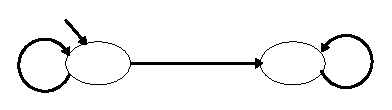
\includegraphics{gg.mem.fin60.eps}%
\end{picture}%
\setlength{\unitlength}{4144sp}%
%
\begingroup\makeatletter\ifx\SetFigFont\undefined%
\gdef\SetFigFont#1#2#3#4#5{%
  \reset@font\fontsize{#1}{#2pt}%
  \fontfamily{#3}\fontseries{#4}\fontshape{#5}%
  \selectfont}%
\fi\endgroup%
\begin{picture}(2724,580)(1631,299)
\put(2197,582){\makebox(0,0)[lb]{\smash{{\SetFigFont{7}{8.4}{\rmdefault}{\mddefault}{\updefault}{\color[rgb]{0,0,0}$v$}%
}}}}
\put(2197,445){\makebox(0,0)[lb]{\smash{{\SetFigFont{7}{8.4}{\rmdefault}{\mddefault}{\updefault}{\color[rgb]{0,0,0}$\emptyset$}%
}}}}
\put(3680,555){\makebox(0,0)[lb]{\smash{{\SetFigFont{7}{8.4}{\rmdefault}{\mddefault}{\updefault}{\color[rgb]{0,0,0}$u$}%
}}}}
\put(3652,418){\makebox(0,0)[lb]{\smash{{\SetFigFont{7}{8.4}{\rmdefault}{\mddefault}{\updefault}{\color[rgb]{0,0,0}$\{p\}$}%
}}}}
\end{picture}%

\end{center}
\caption{A simple turn-based game that demands memoryful strategies}
\label{fig.gg.fin}
\end{figure}

{\lemma \label{lemma.mem.fin}
The strategies of the agents in ATL$^+$ 
(and thus in BSIL) specifications need memory.
This even holds for the single agent case.
\qed 
}


\section{Expressive Power of BSIL}
In this section, we establish that BSIL is incomparable with ATL$^*$, 
AMC, and GL \cite{AHK02} in expressiveness.
In fact, we shall first establish the incomparability between BSIL with 
GL and AMC.  
Then the imcomparability with BSIL follows since GL and AMC are super-classes of 
ATL$^*$ \cite{AHK02}.
\subsection{Comparison with GL}
GL separates strategy quantifications\label{reply1.quantificaitons} from path quantifications.  
In comparison, ATL$^*$ and BSIL combines these two quantifications 
into SQs and SIQs.  
Thus with GL, we can specify that, for all S-profiles of $A$, 
there exists a play saitsfying $\psi_1$.  
The (existential) strategy quantification for agency $A$ 
of GL is of the form $\existsb A.\psi_1$.  
The path quantifications are just ordinary CTL modalities: 
$\forall\pfrr, \forall\until, \exists\pfrr$, and 
$\exists\until$.  

The following two lemmas show the relation between GL and BSIL.  
Lemma~\ref{lemma.gl.cant} uses two inductive families of game graphs 
to show that GL is not as expressive as BSIL. 
The base cases, $G_1$ and $H_1$, are in figure~\ref{fig.gg.exp}
for three agents.
\begin{figure}[t]\begin{center}
\begin{picture}(0,0)%
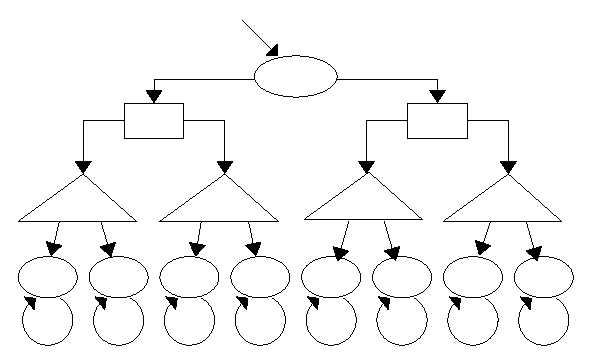
\includegraphics{gg.expba100.eps}%
\end{picture}%
\setlength{\unitlength}{4144sp}%
%
\begingroup\makeatletter\ifx\SetFigFont\undefined%
\gdef\SetFigFont#1#2#3#4#5{%
  \reset@font\fontsize{#1}{#2pt}%
  \fontfamily{#3}\fontseries{#4}\fontshape{#5}%
  \selectfont}%
\fi\endgroup%
\begin{picture}(4250,2496)(169,-1735)
\put(1396,-1276){\makebox(0,0)[lb]{\smash{{\SetFigFont{12}{14.4}{\rmdefault}{\mddefault}{\updefault}{\color[rgb]{0,0,0}$\{q\}$}%
}}}}
\put(3016,-1276){\makebox(0,0)[lb]{\smash{{\SetFigFont{12}{14.4}{\rmdefault}{\mddefault}{\updefault}{\color[rgb]{0,0,0}$\{q\}$}%
}}}}
\put(226,-1276){\makebox(0,0)[lb]{\smash{{\SetFigFont{12}{14.4}{\rmdefault}{\mddefault}{\updefault}{\color[rgb]{0,0,0}$\{p\}$}%
}}}}
\put(2566,-736){\makebox(0,0)[lb]{\smash{{\SetFigFont{12}{14.4}{\rmdefault}{\mddefault}{\updefault}{\color[rgb]{0,0,0}$\{p,q\}$}%
}}}}
\put(3646,-736){\makebox(0,0)[lb]{\smash{{\SetFigFont{12}{14.4}{\rmdefault}{\mddefault}{\updefault}{\color[rgb]{0,0,0}$\{p,q\}$}%
}}}}
\put(1486,-736){\makebox(0,0)[lb]{\smash{{\SetFigFont{12}{14.4}{\rmdefault}{\mddefault}{\updefault}{\color[rgb]{0,0,0}$\{p,q\}$}%
}}}}
\put(406,-736){\makebox(0,0)[lb]{\smash{{\SetFigFont{12}{14.4}{\rmdefault}{\mddefault}{\updefault}{\color[rgb]{0,0,0}$\{p,q\}$}%
}}}}
\put(2071,254){\makebox(0,0)[lb]{\smash{{\SetFigFont{12}{14.4}{\rmdefault}{\mddefault}{\updefault}{\color[rgb]{0,0,0}$\{p,q\}$}%
}}}}
\put(811,-1276){\makebox(0,0)[lb]{\smash{{\SetFigFont{12}{14.4}{\rmdefault}{\mddefault}{\updefault}{\color[rgb]{0,0,0}$\{p\}$}%
}}}}
\put(4051,-1276){\makebox(0,0)[lb]{\smash{{\SetFigFont{12}{14.4}{\rmdefault}{\mddefault}{\updefault}{\color[rgb]{0,0,0}$\{q\}$}%
}}}}
\put(1891,-1276){\makebox(0,0)[lb]{\smash{{\SetFigFont{12}{14.4}{\rmdefault}{\mddefault}{\updefault}{\color[rgb]{0,0,0}$\{q\}$}%
}}}}
\put(2431,-1276){\makebox(0,0)[lb]{\smash{{\SetFigFont{12}{14.4}{\rmdefault}{\mddefault}{\updefault}{\color[rgb]{0,0,0}$\{p\}$}%
}}}}
\put(3511,-1276){\makebox(0,0)[lb]{\smash{{\SetFigFont{12}{14.4}{\rmdefault}{\mddefault}{\updefault}{\color[rgb]{0,0,0}$\{p\}$}%
}}}}
\put(3151,-61){\makebox(0,0)[lb]{\smash{{\SetFigFont{12}{14.4}{\rmdefault}{\mddefault}{\updefault}{\color[rgb]{0,0,0}$\{p,q\}$}%
}}}}
\put(991,-61){\makebox(0,0)[lb]{\smash{{\SetFigFont{12}{14.4}{\rmdefault}{\mddefault}{\updefault}{\color[rgb]{0,0,0}$\{p,q\}$}%
}}}}
\put(2341,524){\makebox(0,0)[lb]{\smash{{\SetFigFont{12}{14.4}{\rmdefault}{\mddefault}{\updefault}{\color[rgb]{0,0,0}$r_0$}%
}}}}
\end{picture}%
\\
(a) $G_1$, a game graph for base case.\\
\begin{picture}(0,0)%
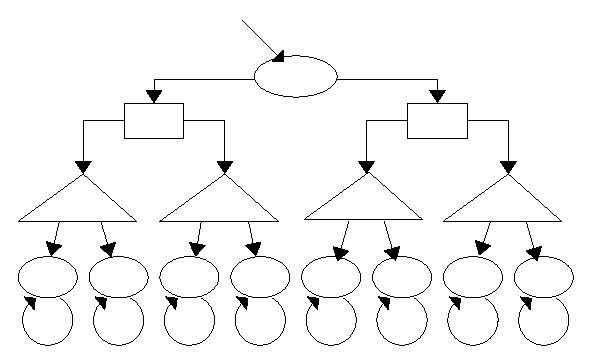
\includegraphics{gg.expbb100.eps}%
\end{picture}%
\setlength{\unitlength}{4144sp}%
%
\begingroup\makeatletter\ifx\SetFigFont\undefined%
\gdef\SetFigFont#1#2#3#4#5{%
  \reset@font\fontsize{#1}{#2pt}%
  \fontfamily{#3}\fontseries{#4}\fontshape{#5}%
  \selectfont}%
\fi\endgroup%
\begin{picture}(4250,2496)(169,-1735)
\put(856,-1276){\makebox(0,0)[lb]{\smash{{\SetFigFont{12}{14.4}{\rmdefault}{\mddefault}{\updefault}{\color[rgb]{0,0,0}$\{p\}$}%
}}}}
\put(1396,-1276){\makebox(0,0)[lb]{\smash{{\SetFigFont{12}{14.4}{\rmdefault}{\mddefault}{\updefault}{\color[rgb]{0,0,0}$\{p\}$}%
}}}}
\put(3016,-1276){\makebox(0,0)[lb]{\smash{{\SetFigFont{12}{14.4}{\rmdefault}{\mddefault}{\updefault}{\color[rgb]{0,0,0}$\{q\}$}%
}}}}
\put(3556,-1276){\makebox(0,0)[lb]{\smash{{\SetFigFont{12}{14.4}{\rmdefault}{\mddefault}{\updefault}{\color[rgb]{0,0,0}$\{p\}$}%
}}}}
\put(226,-1276){\makebox(0,0)[lb]{\smash{{\SetFigFont{12}{14.4}{\rmdefault}{\mddefault}{\updefault}{\color[rgb]{0,0,0}$\{p\}$}%
}}}}
\put(2566,-736){\makebox(0,0)[lb]{\smash{{\SetFigFont{12}{14.4}{\rmdefault}{\mddefault}{\updefault}{\color[rgb]{0,0,0}$\{p,q\}$}%
}}}}
\put(3646,-736){\makebox(0,0)[lb]{\smash{{\SetFigFont{12}{14.4}{\rmdefault}{\mddefault}{\updefault}{\color[rgb]{0,0,0}$\{p,q\}$}%
}}}}
\put(1486,-736){\makebox(0,0)[lb]{\smash{{\SetFigFont{12}{14.4}{\rmdefault}{\mddefault}{\updefault}{\color[rgb]{0,0,0}$\{p,q\}$}%
}}}}
\put(406,-736){\makebox(0,0)[lb]{\smash{{\SetFigFont{12}{14.4}{\rmdefault}{\mddefault}{\updefault}{\color[rgb]{0,0,0}$\{p,q\}$}%
}}}}
\put(2071,254){\makebox(0,0)[lb]{\smash{{\SetFigFont{12}{14.4}{\rmdefault}{\mddefault}{\updefault}{\color[rgb]{0,0,0}$\{p,q\}$}%
}}}}
\put(4051,-1276){\makebox(0,0)[lb]{\smash{{\SetFigFont{12}{14.4}{\rmdefault}{\mddefault}{\updefault}{\color[rgb]{0,0,0}$\{q\}$}%
}}}}
\put(3151,-106){\makebox(0,0)[lb]{\smash{{\SetFigFont{12}{14.4}{\rmdefault}{\mddefault}{\updefault}{\color[rgb]{0,0,0}$\{p,q\}$}%
}}}}
\put(991,-106){\makebox(0,0)[lb]{\smash{{\SetFigFont{12}{14.4}{\rmdefault}{\mddefault}{\updefault}{\color[rgb]{0,0,0}$\{p,q\}$}%
}}}}
\put(1891,-1276){\makebox(0,0)[lb]{\smash{{\SetFigFont{12}{14.4}{\rmdefault}{\mddefault}{\updefault}{\color[rgb]{0,0,0}$\{q\}$}%
}}}}
\put(2431,-1276){\makebox(0,0)[lb]{\smash{{\SetFigFont{12}{14.4}{\rmdefault}{\mddefault}{\updefault}{\color[rgb]{0,0,0}$\{q\}$}%
}}}}
\put(2296,524){\makebox(0,0)[lb]{\smash{{\SetFigFont{12}{14.4}{\rmdefault}{\mddefault}{\updefault}{\color[rgb]{0,0,0}$s_0$}%
}}}}
\end{picture}%
\\
(b) $H_1$, another game graph for base case.\\
$\bigcirc$ belongs to Agent  1; $\pfrr$ belongs to Agent 2; and 
$\triangle$ belongs to Agent 3.
\end{center}
\caption{Base cases for the expressiveness of BSIL over ATL$^*$}
\label{fig.gg.exp}
\end{figure}
The inductive cases, $G_{k+1}$ and $H_{k+1}$, are 
respectively constructed out of $G_k$ and $H_k$ as 
in figure~\ref{fig.gg.expi}.
\begin{figure}[t]\begin{center}
\begin{picture}(0,0)%
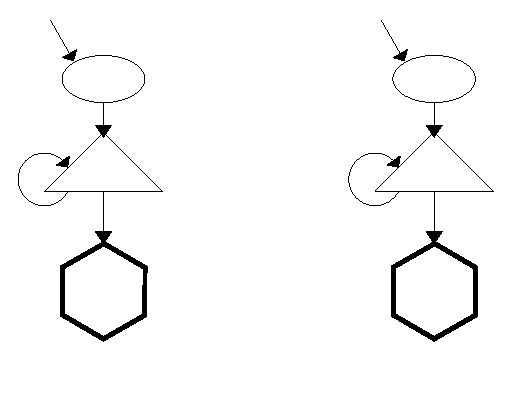
\includegraphics{gg.expi100.eps}%
\end{picture}%
\setlength{\unitlength}{4144sp}%
%
\begingroup\makeatletter\ifx\SetFigFont\undefined%
\gdef\SetFigFont#1#2#3#4#5{%
  \reset@font\fontsize{#1}{#2pt}%
  \fontfamily{#3}\fontseries{#4}\fontshape{#5}%
  \selectfont}%
\fi\endgroup%
\begin{picture}(3643,2925)(1635,-2164)
\put(1891,-2086){\makebox(0,0)[lb]{\smash{{\SetFigFont{12}{14.4}{\rmdefault}{\mddefault}{\updefault}{\color[rgb]{0,0,0}(a) $G_k$}%
}}}}
\put(4411,-2086){\makebox(0,0)[lb]{\smash{{\SetFigFont{12}{14.4}{\rmdefault}{\mddefault}{\updefault}{\color[rgb]{0,0,0}(b) $H_k$}%
}}}}
\put(2116,-1366){\makebox(0,0)[lb]{\smash{{\SetFigFont{12}{14.4}{\rmdefault}{\mddefault}{\updefault}{\color[rgb]{0,0,0}$G_{k-1}$}%
}}}}
\put(4636,-1366){\makebox(0,0)[lb]{\smash{{\SetFigFont{12}{14.4}{\rmdefault}{\mddefault}{\updefault}{\color[rgb]{0,0,0}$H_{k-1}$}%
}}}}
\put(2071,-466){\makebox(0,0)[lb]{\smash{{\SetFigFont{12}{14.4}{\rmdefault}{\mddefault}{\updefault}{\color[rgb]{0,0,0}$\{p,q\}$}%
}}}}
\put(4591,-466){\makebox(0,0)[lb]{\smash{{\SetFigFont{12}{14.4}{\rmdefault}{\mddefault}{\updefault}{\color[rgb]{0,0,0}$\{p,q\}$}%
}}}}
\put(4591,254){\makebox(0,0)[lb]{\smash{{\SetFigFont{12}{14.4}{\rmdefault}{\mddefault}{\updefault}{\color[rgb]{0,0,0}$\{p,q\}$}%
}}}}
\put(2071,254){\makebox(0,0)[lb]{\smash{{\SetFigFont{12}{14.4}{\rmdefault}{\mddefault}{\updefault}{\color[rgb]{0,0,0}$\{p,q\}$}%
}}}}
\put(2251,524){\makebox(0,0)[lb]{\smash{{\SetFigFont{12}{14.4}{\rmdefault}{\mddefault}{\updefault}{\color[rgb]{0,0,0}$r_k$}%
}}}}
\put(4816,524){\makebox(0,0)[lb]{\smash{{\SetFigFont{12}{14.4}{\rmdefault}{\mddefault}{\updefault}{\color[rgb]{0,0,0}$s_k$}%
}}}}
\end{picture}%
\\
$\bigcirc$ belongs to Agent  1; $\pfrr$ belongs to Agent 2; and 
$\triangle$ belongs to Agent 3.
\end{center}
\caption{Inductive cases for the expressiveness of BSIL over ATL$^*$}
\label{fig.gg.expi}
\end{figure}


{\lemma \label{lemma.gl.cant}
Every GL formula $\phi$ with $k$ ($k>0$) SQs cannot distinguish 
$G_k$ and $H_k$ while 
$\langle 1\rangle ((\langle+ 2\rangle\pfrr p)
    \wedge \langle+ 2\rangle\pfrr q)$ can.
}
\\\pf 
It is clear that
$\langle 1\rangle ((\langle+ 2\rangle \pfrr p)
    \wedge (\langle+ 2\rangle \pfrr q))$ can $G_k$ and $H_k$ 
no matter what value $k$ is.  
The proof continues by an induction $k$, the numbrer of SQs in $\phi$. 

\noindent 
{\bf Base case:} Assume that $\phi$ has only one modal operator.
Then there are the following case analysis of GL formulas.
\begin{list1}
\item {\bf Case 1:} {\em $\phi$ is $\existsb  A.\phi_1$
    where $\phi_1$ is a Boolean combination of
    formulas of the form $\exists \psi$ or $\forall \psi$
    where $\psi$ is a path formula.}
    Note that $\phi_1$ characterizes a set of states that 
    either start a play satisfying $\psi$ or 
    start only plays satisfying $\psi$.
    The following case analysis shows that, for every
    trace subset $S$ and every agency $A$,
    there exists a strategy of $A$ to characterize
    $S$ in figure~\ref{fig.gg.exp}(a) iff
    there exists a strategy for $A$ to characterize
    $S$ in figure~\ref{fig.gg.exp}(b).
    \begin{list2}
    \item {\bf Case 1a:} {\em $\phi$ is $\existsb\emptyset.\phi_1$.}
        In this case, there is no strategy and the sets of traces
        imposed by no strategy in the two state graphs are
        both $\{\pfrr p,\pfrr q\}$.
        Thus, $\existsb\emptyset.\phi_1$ cannot distinguish the trace sets of the
        two state graphs.
    \item {\bf Case 1b:} {\em $\phi$ is $\existsb\{1\}.\phi_1$.}
        From figure~\ref{fig.gg.exp}, no matter what strategies
        agency $\{1\}$ may choose, the
        trace sets for the two game graphs are both
        $\{\pfrr p,\pfrr q\}$.
        Thus, $\existsb\{1\}.\phi_1$ cannot distinguish the trace sets of the
        two state graphs.
    \item {\bf Case 1c:} {\em $\phi$ is
        $\existsb\{2\}.\phi_1$.}
        This case is similar to case 1b.
    \item {\bf Case 1d:} {\em $\phi$ is
        $\existsb\{3\}.\phi_1$.}
        This case is similar to case 1b.
    \item {\bf Case 1e:} {\em $\phi$ is
        $\existsb\{1,2\}.\phi_1$.}
        Agency $\{1, 2\}$ can cooperate to force three trace sets:
        $\{\pfrr p\}, \{\pfrr q\}, \{\pfrr p,\pfrr q\}$
        in both of the game graphs in figure~\ref{fig.gg.exp}.
        Thus, $\existsb\{1,2\}.\phi_1$ cannot distinguish the trace sets of the
        two state graphs.
    \item {\bf Case 1f:} {\em $\phi$ is
        $\existsb\{1,3\}.\phi_1$.}
        This case is similar to case 1e.
    \item {\bf Case 1g:} {\em $\phi$ is
        $\existsb\{2,3\}.\phi_1$.}
        This case is similar to case 1e.
    \item {\bf Case 1h:} {\em $\phi$ is
        $\existsb\{1,2,3\}.\phi_1$.}
        Agency $\{1, 2,3\}$ can cooperate to force three trace sets:
        $\{\pfrr p\}, \{\pfrr q\}, \{\pfrr p,\pfrr q\}$
        in both of the game graphs in figure~\ref{fig.gg.exp}.
        Thus, $\existsb\{1,2,3\}.\phi_1$ cannot distinguish the trace sets of the
        two state graphs.
    \end{list2}
\item {\bf Case 2:} {\em $\phi$ is a Boolean combination of
    formulas in case 1.}
    Since case 1 does not distinguish the two game graphs, 
    this case can neither do it.  
\end{list1}
Thus the base case is proven.

\noindent {\bf Induction step:}
If $\phi$ has $k$ modal operators,
to tell the difference between $G_k$ and $H_k$,
we need a modal subformula of $\phi$ that can tell the difference
of $G_{k-1}$ and $H_{k-1}$.
But according to the inductive hypothesis, this is impossible.
Thus the lemma is proven.  
\qed 



{\lemma \label{lemma.gl.incomp}
GL formula $\existsb\{1\}.((\exists\pfrr p)\wedge\exists\pfrr q)$
is not equivalent to any BSIL formula.
}
\\\pf The proof basically follows the same argument in \cite{AHK02} 
that $\existsb\{1\}.((\exists\pfrr p)\wedge\exists\pfrr q)$ 
is not equivalent to 
any ATL$^*$ formula.  
\qed 

Lemmas~\ref{lemma.gl.cant} and 
\ref{lemma.gl.incomp} together show that 
GL and BSIL are not comparable in expressiveness.  
\subsection{Comparison with AMC}
AMC is an extension from $\mu$-calculus and allows 
for multiple fixpoints interleaved together \cite{AHK02}.  
An AMC formula contains fixpoint operators on state set variables.  
The only modality of AMC is of the form $\langle A\rangle\nxt\psi$ 
and least fixpoint $\emlfp x.\psi_1(x)$ where 
$\psi_1(x)$ is a Boolean function of atomic propositions 
and state set variables (including $x$).  
It is required that every occurrence of $x$ in $\psi_1$ is 
under even number of negations.  
The duality of the least fixpoint operator is the greatest fixpoint 
operator $\emgfp$.  
Formula $\emgfp x.\psi_1$ is defined as $\neg\emlfp x.\neg\psi_1(x)$.  

To establish that AMC is not as expressive as BSIL, we basically follow 
the proof style for Lemma~\ref{lemma.atl.cant} and 
use the same two families of game graphs.  
% (See appendix~\ref{app.lemma.atl.cant}).  
The statement of the lemma requires notations for 
state set variables and other details in AMC. 
We need to define the domain of values for the free state set variables 
in AMC formulas.  
Let $X$ be the set of state set variables.  
Without loss of generality, we assume that no two subformulas
of the form $\emlfp x.\phi$ in
a given AMC formula share the same quantified name of $x$.
Given a subformula $\emlfp x_i.\phi$
with free variables $x_1,\ldots,x_n$ in $\phi$
and no modal operator $\langle\ldots\rangle\nxt$ in $\phi$,
we define $\phi$ as a {\em base template} for $x_i$.
Then we can define the {\em base formula domain} of $x_i$,
denoted $F_0(x_i)$,
as the smallest set with the following restrictions.
We let $\phi[x_1\mapsto \eta_1,\ldots,x_n\mapsto\eta_n]$ 
be the AMC formula identical to 
$\phi$ except that every occurrence of $x_i$ in $\phi$ are respectively 
replaced with $\eta_i$.  
\begin{list1}
\item For each $x_i\in X$ with base template $\phi$,
    $\phi[x_1\mapsto\false,\ldots,x_n\mapsto\false]\in F_0(x_i)$.
\item For each $x_i\in X$ with base template $\phi$
    and $\phi_1\in F_0(x_1),\ldots,\phi_n\in F_0(x_n)$,
    $\phi[x_1\mapsto\phi_1,\ldots,x_n\mapsto\phi_n]\in F_0(x_i)$.
\end{list1}
Note that there is neither variables nor `$\emlfp$' operators
in $F_0(x)$ for every $x$.
Thus we can define the characterization $\kappa$ 
of a formula $\phi_1$ in $F_0(x)$ for $\calg$,
in symbols $\kappa(\calg,\phi_1)$, as follows.
\begin{list1}
\item For each atomic proposition $p\in P$,
    $\kappa(\calg,p)=\{q\mid p\in\lambda(q)\}$.
\item For each $\phi\in F_0(x)$, 
    $\kappa(\calg,\neg\phi)=Q-\kappa(\calg,\phi)$.
\item For each $\phi_1,\phi_2\in F_0(x)$,
    $\kappa(\calg,\phi_1\vee\phi_2)=\kappa(\calg,\phi_1)\cup\kappa(\calg,\phi_2)$.
\end{list1}
A {\em valuation} $\nu$ of variables in $X$ for $\calg$
is a mapping from
$X$ such that, for each $x\in X$, there exists a base domain formula
$\phi$ of $x$ such that $\nu(x)= \kappa(\calg,\phi)$.

The expressiveness comparison between AMC and BSIL relies on the
following lemma.

{\lemma \label{lemma.amc.domain}
For every AMC formula $\phi$ without modal operator of the
form $\langle\ldots\rangle\nxt$, state set variable $x$, and
a formula $\phi_1$ in $F_0(x)$,
$r_0\in\kappa(G_0,\phi_1)$
iff
$s_0\in\kappa(H_0,\phi_1)$
in figure~\ref{fig.gg.exp}.
}
\\\pf 
We can prove this with an structural induction on $\phi_1$.
The base case is straightforward.
The inductive step follows since Boolean combinations of
subformulas that cannot distinguish $G_0$ and $H_0$ can neither
distinguish the two game graphs.
\qed


Now we want to classify AMC formulas according to the nesting depths of
operators of the form $\langle\ldots\rangle\nxt$ in a formula.
Specifically, we let $\mbox{AMC}^{(k)}$ be the set of AMC formulas
with exactly nesting depth $k$ of operator $\langle \ldots\rangle\nxt$.
For example,
$\emlfp x.\langle 1\rangle \nxt
(p\rightarrow \emlfp y.\langle 2\rangle (x\vee y\wedge\nxt q))$
is in $\mbox{AMC}^{(2)}$.
Then, $\mbox{AMC}^{(0)}$ is
the smallest set with the following restrictions.
\begin{list1}
\item {\bf Case 1a:} For each atomic proposition $p\in P$,
    $p\in \mbox{AMC}^{(0)}$.
\item {\bf Case 1b:} For each proposition variable $x\in X$,
    $x\in \mbox{AMC}^{(0)}$.
\item {\bf Case 1c:} For each $\phi\in \mbox{AMC}^{(0)}$,
    $\neg\phi\in \mbox{AMC}^{(0)}$.
\item {\bf Case 1d:} For each $\phi_1,\phi_2\in \mbox{AMC}^{(0)}$,
    $\phi_1\vee\phi_2\in \mbox{AMC}^{(0)}$.
\item {\bf Case 1e:} For each $\phi\in \mbox{AMC}^{(0)}$ and
    proposition variable $x\in X$,
    $\emlfp x.\phi\in \mbox{AMC}^{(0)}$.
\end{list1}
Then $\mbox{AMC}^{(k)}$, $k>0$,
is the smallest set with the following restrictions.
\begin{list1}
\item {\bf Case 2a:} For each $A\subseteq [1,m]$ and
    $\phi\in \mbox{AMC}^{(k-1)}$,
    $\langle A\rangle \nxt \phi\in \mbox{AMC}^{(k)}$,
\item {\bf Case 2b:} For each $\phi\in \mbox{AMC}^{(k)}$,
    $\neg\phi\in \mbox{AMC}^{(k)}$.
\item {\bf Case 2c:} For each $\phi_1\in \mbox{AMC}^{(k)}$ and
    $\phi_2\in\bigcup_{h\leq k}\mbox{AMC}^{(h)}$,
    $\phi_1\vee\phi_2\in \mbox{AMC}^{(k)}$.
\item {\bf Case 2d:} For each
    $\phi_1\in\bigcup_{h\leq k}\mbox{AMC}^{(h)}$ and $\phi_2\in \mbox{AMC}^{(k)}$,
    $\phi_1\vee\phi_2\in \mbox{AMC}^{(k)}$.
\item {\bf Case 2e:} For each $\phi\in \mbox{AMC}^{(k)}$ and
    proposition variable $x\in X$,
    $\emlfp x.\phi\in \mbox{AMC}^{(k)}$.
\end{list1}
Note that there could be free variables in the formulas classified in
the above.
The evaluation of such formulas for a game graph depends on the
valuation of the free variables.

Given two game graphs $G,H$ and
an AMC formulas $\phi$,
we say that
two valuations of $\nu$ and $\nu'$ respectively of $G$ and $H$
are {\em consistent} if for every $x\in X$,
there exists a $\phi_1\in F_0(x)$ such that
$\nu(x)=\kappa(G,\phi_1)$ and $\nu'(x)=\kappa(H,\phi_1)$.
In the following, we adopt the AMC semantic notations in \cite{AHK02}.
Given a game graph $G$, an AMC formula $\phi$,
and a valuation $\nu$ of state set variables in $X$,
$(\phi)^G(\nu)$ denotes the set of states of $G$ that
satisfy $\phi$ with valuation $\nu$.







{\lemma\label{lemma.amc.induction}
Assume that $G_k$ and $H_k$ are defined in
figures~\ref{fig.gg.exp} and \ref{fig.gg.expi}.
For every $k$, AMC formula $\phi\in \mbox{AMC}^{(k)}$, and two consistent
valuations $\nu$ and $\nu'$ respectively of $G_k$ and $H_k$,
$r_k\in (\phi)^{G_k}(\nu)$ iff
$s_k\in (\phi)^{H_k}(\nu')$.
}
\\\pf
We use an induction on $k$ to prove the lemma.

\noindent
{\bf Base case:} 
When $\phi$ is in case 1a through 1d, the lemma follows straightforwardly.
In case 1e,
$(\emlfp x.\psi)^{G_1}(\nu)$ can be expanded as follows.
We let
\begin{list1}
\item $\psi^{G_1,\nu,(0)}$ be $(\psi[x\mapsto \false])^{G_1}(\nu)$ and
\item for each $h>0$,
    $\psi^{G_1,\nu,(h)}$ be $(\phi[x\mapsto \psi_1^{G_1,(h-1)}])(\nu)$.
\end{list1}
Then $(\emlfp x.\phi)^{G_1}(\nu)=\bigcup_{h\geq 0}\psi^{G_1,\nu,(h)}$
according to the semantics of AMC.
Similarly, \linebreak 
$(\emlfp x.\phi)^{H_1}(\nu')=\bigcup_{h\geq 0}\psi^{H_1,\nu',(h)}$.
According to the same argument for cases 1a through 1d,
for each $h\geq 0$,
$r_0\in \psi^{G_1,\nu,(h)}$ iff
$s_0\in \psi^{H_1,\nu',(h)}$.
Thus it is clear that
$r_0\in (\emlfp x.\phi)^{G_1}(\nu)$ iff
$s_0\in (\emlfp x.\phi)^{H_1}(\nu')$.
Thus the lemma is proven in this case.

\noindent
{\bf Induction step:}
To tell the difference between $G_k$ and $H_k$,
we need a formula with the following structure.
\begin{list1}
\item At least one nesting of operators
    like $\langle\ldots\rangle\nxt$ in a least fixpoint operation 
    to infer the reachability of $G_{k-1}$ and $H_{k-1}$.
\item A modal subformula nested inside a $\langle \ldots\rangle \nxt$
    modal operator of $\phi$ that can tell the difference
    of $G_{k-1}$ and $H_{k-1}$.  
    But according to the inductive hypothesis, this is impossible.  
\end{list1}
Thus the lemma is proven.
\qed


Then with Lemma~\ref{lemma.amc.induction}, 
we conclude the proof for Lemma~\ref{lemma.amc.cant} in the following. 


{\lemma \label{lemma.amc.cant}
For every AMC formula $\phi$,
there are two game graphs that
$\phi$ cannot distinguish while
$\langle 1\rangle ((\langle+ 2\rangle\pfrr p)
    \wedge \langle+ 2\rangle\pfrr q)$ can.
}
\\\pf 
In the proof for Lemma~\ref{lemma.amc.induction}, 
it is apparent that $\phi$ with $\phi\in\mbox{AMC}^{(k)}$ cannot 
tell $G_k$ and $H_k$.  
\qed 

By the same argument in \cite{AHK02}, 
for one-agent game, BSIL coincides with CTL and is not as expressive as 
AMC. 

{\lemma \label{lemma.amc.can}
For game graphs of one agent,
AMC is strictly more expressive than BSIL.} 
\\\pf 
For one-agent games, 
AMC is equivalent to $\mu$-calculus and BSIL is equivalent to CTL which
is strictly less expressive than $\mu$-calculus.
\qed 



A comment on Lemmas~\ref{lemma.gl.cant} and \ref{lemma.amc.cant} 
is that the path modal formulas in the lemmas can be changed 
independently to $\pevt \neg p$ and $\pevt \neg q$ without affecting the validity of 
the lemma.  
This can be used to show that the example properties in the introduction 
are indeed inexpressible in ATL$^*$, GL, and AMC.  

\subsection{Comparison with ATL*}
It is easy to see that BSIL is a super-class of ATL.
Thus we have the following lemma.

{\lemma \label{lemma.atl.less}
BSIL is at least as expressive as ATL.  
}
% \\\pf The lemma is true since BSIL without SIQs coincides with ATL.  
\qed

Then Lemmas~\ref{lemma.gl.cant} and \ref{lemma.amc.cant} 
lead to the 
fact that there are some BSIL properties that 
ATL$^*$ cannot express 
since GL and AMC are both super-class of ATL$^*$ \cite{AHK02}.  



{\lemma \label{lemma.atl.cant} 
For every ATL$^*$ formula $\phi$, 
there are two game graphs that
$\phi$ cannot distinguish while
$\langle 1\rangle ((\langle+ 2\rangle\pfrr p)
    \wedge \langle+ 2\rangle\pfrr q)$ can.
}\qed 

Lemmas~\ref{lemma.atl.less} and \ref{lemma.atl.cant} together establish  
that ATL is strictly less expressive than BSIL. 
Then the following lemma shows the reverse direction.  

{\lemma \label{lemma.atl.incomp}
ATL$^*$ formula $\langle 1\rangle\pfrr\pevt p$
is not equivalent to any BSIL formula.
} 
\\\pf 
The proof is similar to the proof for the inexpressibility of 
$\langle 1\rangle\pfrr\pevt p$ with ATL \cite{AHK02}.  
\qed 

Lemmas~\ref{lemma.atl.cant} and \ref{lemma.atl.incomp}
together establish  
that ATL$^*$ and BSIL are not comparable in expressiveness. 

\section{Algorithm and Complexity}
The model-checking problem of BSIL is contained in 
PSPACE mainly due to the restriction that disallows 
negation in tree formulas.
As in the model-checking algorithms 
of ATL \cite{AHK02}, we can evaluate the proper state subformulas \label{reply1.subformulas.formulas} 
independently and then treat them as auxiliary propositions.  
Moreover, as in the evaluation of $\pevt$-formulas in 
ATL model-checking, 
if a $\pevt$-formula can be enforced with an S-profile, it can be enforced 
in a finite number of steps along every play compatible with 
the strategy in a computation tree.  
Once a bound $b$ for this finite number of steps is determined, 
we can enumerate all strategies embedded in the computation 
tree up to depth $b$ and try to find one that enforces a BSIL formula.  

\label{reply2.exp.alg2} 
As explained in section~\ref{sec.running}, 
our algorithm also labels subformulas and their symbolic S-profiles 
on the nodes in a computation tree. 
The formula is satisfied if and only if we can 
find a finite tree top with labels consistent with the SQs and SIQs in the input formula 
and can be extended to an infinite computation tree. 
In Subsection~\ref{subsec.children.ltl.ob},
we derive the labels, i.e., subformulas and their symbolic S-profiles, that are 
sufficient for our model-checking algorithm and 
present two procedures: 
\begin{list1} 
\item \tteval() that checks whether the satisfaction of formulas at a state 
	can be decided locally.  
\item \ttsynsuc() that nondeterministically chooses a scheme to 
	pass down the subformulas and their symbolic S-profiles to the child nodes 
	without violating the restrictions on the S-profiles declared with the SQs and SIQs. 
\end{list1} 

There are, however, severe differences between exploring 
a computation tree for 
BSIL and exploring one for ATL \cite{AHK02}.   
For BSIL, we have to take the interaction of strategies into account.  
For example, we may have to enforce a subformula 
$\langle 1\rangle((\langle+ 2\rangle \pevt p)
\wedge\langle+ 2\rangle (\pfrr q\vee \pevt r))$.  
Then, when exploring the computation tree, 
we may follow two strategies of Agent 2, one to enforce $\pevt p$ and 
the other to enforce $\pfrr q$ or $\pevt r$.  
There are the following situation for the 
interaction between these two strategies. 
The two strategies may make the same decision all the way 
until we reach a tree node $v$.  
(For turn-based games, $v$ has to be owned by Agent 2.)    
This can be conceptualized as passing the obligations of $\pevt p$ and 
$\pfrr q\vee\pevt r$ along the path from the root to $v$.  
Then, at node $v$, the two strategies may differ in their decisions 
and pass down the two obligations to different branches. 

\label{reply2.exp.alg3} 
Then, in Subsection~\ref{subsec.alg.proc},
we present our algorithm in two parts,
one for model-checking BSIL state formulas
and the other for model-checking BSIL tree formulas.
In Subsection~\ref{subsec.alg.corr},
we prove the correctness of the algorithm.
In Subsection~\ref{subsec.alg.pspace}, 
we show that our algorithm is in PSPACE.  
Together with Lemma~\ref{lemma.bsil.mck.nphard} in 
Subsection~\ref{subsec.pspace.hard}, 
we then establish the PSPACE-completeness of 
the BSIL and ATL$^+$ model-checking problems.  



\subsection{Computing path obligations and passing them down the computation tree
\label{subsec.children.ltl.ob}
}

We use $\{a_1 \mapsto s_1,\ldots,a_n\mapsto s_n\}$ to denote 
a partial function that maps $a_i$ to $s_i$ for each $i\in[1,n]$.  
Given a partial function $f$, 
we denote the domain of $f$ by $\emdef(f)$.
Inheriting the notations in \cite{MMV10}, 
we may also represent the the mapping as $(a_1,s_1)(a_2,s_2)\ldots(a_n,s_n)$.  
% be the set of domain elements that 
% is defined with $\zeta$.  

We need some special techniques in checking tree formulas.  
We adopt the concept of strategy variables from \cite{CHP10,MMV10}. 
A {\em strategy variable binding} ({\em SV-binding} for short) 
is a partial function from $[1,m]$ to strategy variables.  
Given an SV-binding $\Lambda$, 
$\Lambda\circ(a_1, s_1)\ldots(a_n, s_n)$ 
is the SV-binding that is identical to $\Lambda$ 
except that Agent $a_i$ is bound to $s_i$ for every $i\in[1,n]$.  
% Given an agency $A\subseteq[1,m]$, 
% $\Lambda^{\neg A}$ is defined the same as $\Lambda$ on $[1,m]- A$.  
% That is, 
% $\Lambda^{\neg A}$ is 
% $\{a\mapsto s\mid a\mapsto s\in \Lambda,a\not\in A\}$.  

Suppose that we are given SV-bindings $\Lambda_1,\ldots,\Lambda_n$
and S-profiles $\Sigma_1,\ldots,\Sigma_n$.   
We say that $\Lambda_1,\ldots,\Lambda_n$ {\em matches} 
$\Sigma_1,\ldots,\Sigma_n$ if, and only if, 
for every $a\in[1,m]$ and $i,j\in[1,n]$ 
with $a\in\emdef(\Sigma_i)\cap\emdef(\Sigma_j)$, 
$\Sigma_i(a)=\Sigma_j(a)$ if, and only if, 
$\Lambda_i(a)=\Lambda_j(a)$.  

Given an SV-binding $\Lambda$ 
and a state, tree, or path formula $\psi$, 
$\Lambda\psi$ is called a {\em bound formula}.  
$\Lambda\psi$ is a {\em bound path obligation} ({\em BP-constraint}) 
if $\psi$ is a Boolean combination of path formulas.  
A Boolean combination of BP-obligations is called a 
{\em Boolean bound formula} ({\em BB-formula}).  
The strategy variables in BB-formula are only used to tell 
whether or not two path properties are to be enforced with the same strategy.  
For example, the property  
$\langle 1\rangle((\langle+ 2\rangle\pevt p)\wedge 
\langle+ 2\rangle(\pfrr q\vee\pevt r))$ 
can be rewritten as BB-formula 
$((1, s_1)(2,s_2)\pevt p)\wedge 
(1, s_1)(2, s_3)\pfrr q\vee\pevt r$, which says that 
Agent 1 must use the same strategy to fulfill  
both $\pevt p$ and $\pfrr q\vee\pevt r$, while 
Agent 2 may use different strategies to fulfill these two path 
properties.  


Suppose we are given a function $\pi$ that maps symbolic strategy 
names to strategies.  
Similar to the semantics of 
strategy logics \cite{MMV10} with strategy variables, 
we can also define the satisfaction of BB-formulas 
$\Lambda\psi$ at a state $q$ with $\pi$, 
in symbols $\calg,q\models^\pi\Lambda\psi$,  
as follows. 
\begin{list1} 
\item $\calg,q\models^\pi \Lambda_1\psi_1\vee\Lambda_2\psi_2$ iff 
	$\calg,q\models^\pi \Lambda_1\phi_1$ or 
	$\calg,q\models^\pi \Lambda_2\phi_2$ holds. 
\item $\calg,q\models^\pi \Lambda_1\phi_1\wedge\Lambda_2\phi_2$ iff both 
	$\calg,q\models^\pi \Lambda_1\phi_1$ and  
	$\calg,q\models^\pi \Lambda_2\phi_2$ hold. 
\item Given an SV-binding $\Lambda$ and a path formula $\psi_1$ with  
	an S-profile 
	$\Sigma=\{a\mapsto \pi(\Lambda(a))\mid a\in\emdef(\Lambda)\}$, 
	$\calg,q\models^\pi \Lambda\psi_1$ iff, for all plays $\rho$ 
	compatible with $\Sigma$ from $q$, 
	$\rho\models_\Sigma \psi_1$ holds. 
\end{list1} 
In Table~\ref{tab.bbf.rewrite}, 
we present equivalence rules to rewrite state, tree, and path 
formulas to BB-formulas 
using the procedure $\embf()$.  
\begin{table*}[t!]
\caption{Rewriting rules for BB-formulas}
\label{tab.bbf.rewrite}
\begin{center}
% \hspace*{10mm} 
$\begin{array}{lcl} 
\embf(\Lambda\neg\neg\phi) 
& \equiv & \embf(\Lambda\phi)\\
\embf(\Lambda(\tau_1\vee\tau_2)) 
& \equiv & \embf(\Lambda \tau_1)\vee\embf(\Lambda \tau_2)\\
\embf(\Lambda(\tau_1\wedge\tau_2)) 
& \equiv & \embf(\Lambda\tau_1)\wedge\embf(\Lambda\tau_2)\\
\embf(\Lambda \langle a_1,\ldots,a_n\rangle\psi) 
& \equiv & \embf(\{a_1\mapsto \emnewv(), \ldots, a_n\mapsto \emnewv()\}\psi)\\
\embf(\Lambda \langle+ a_1,\ldots,a_n\rangle\psi) 
& \equiv & \embf(\Lambda\circ\{a_1\mapsto \emnewv(), \ldots, a_n\mapsto \emnewv()\}\psi)\\
\embf(\Lambda \nxt\phi_1) 
& \equiv & \Lambda\nxt\embf(\emptyset\phi_1)\\
\embf(\Lambda \neg\nxt\phi_1) 
& \equiv & \Lambda\nxt\embf(\emptyset\neg\phi_1)\\
\embf(\Lambda \phi_1\until\phi_2) 
& \equiv & \Lambda\embf(\emptyset\phi_1)\until\embf(\emptyset\phi_2)\\
\embf(\Lambda \neg\phi_1\until\phi_2) 
& \equiv & \Lambda((\embf(\emptyset\phi_1)
	\until\embf(\neg\emptyset(\phi_1\vee\phi_2)))
           \vee \pfrr\embf(\emptyset\neg\phi_2))\\
\embf(\Lambda p) \equiv p 
&;  & \embf(\Lambda \neg p) \equiv \neg p\\
\embf(\Lambda \true) \equiv \true
&;  & \embf(\Lambda \neg\true) \equiv \false\\
\embf(\Lambda \false) \equiv \false
&;  & \embf(\Lambda \neg\false) \equiv \true\\
\end{array}$\\
$\phi_1,\phi_2$: state or path formulas.  
$\tau_1,\tau_2$: tree formulas.
$\psi_1,\psi_2$: tree or path formulas.
\end{center} 
\end{table*}
For convenience, we use a procedure $\emnewv()$ that returns a
strategy variable that has not been used before.  
In general, the semantics of BSIL deals with the satisfaction 
of a set of subformulas bound to different S-profiles.  
The following two lemmas relate the 
rules in Table~\ref{tab.bbf.rewrite} 
with the semantics of BSIL formulas.  


{\lemma \label{lemma.bbf.fwd}
Suppose we are given a state $q$, 
a BSIL subformula $\psi$, and 
a S-profile $\Sigma$ such that $\calg,q\models_\Sigma\psi$.  
There exist an SV-binding $\Lambda$ and a function $\pi$ such that 
$\calg,q\models^\pi\embf(\Lambda\psi)$.  
} 
\\\pf 
We construct $\Lambda$ and $\pi$ as follows. 
Without loss of generality, 
we assume $\psi$ is unique in the input formula. 
For every $a\in\emdef(\Sigma)$, 
we let $\Lambda(a)=s_a^\psi$ and $\pi(s_a^\psi)=\Sigma(a)$.  
It is clear that the functional composition of $\Lambda$ and $\pi$ is actually $\Sigma$.   
Then, according to the semantics of 
$\calg,q\models^\pi\embf(\Lambda\psi)$ presented in the above, 
$\calg,q\models^\pi\embf(\Lambda\psi)$ since 
for all play $\rho$ compatible with $\Sigma$ from $q$, 
$\rho\models_\Sigma\psi$.  
Thus the lemma is proven. 
\qed 

{\lemma \label{lemma.bbf.bkd}
Suppose we are given a state $q$,
a BSIL subformula $\psi$, 
a SV-bindings $\Lambda$, 
and a function $\pi$ such that  
$\calg,q\models^\pi\embf(\Lambda\psi)$.  
Then there exist an S-profile $\Sigma$ 
such that $\calg,q\models_\Sigma\psi$. 
}
\\\pf 
We can construct $\Sigma$ by 
defining, for all $a\in \emdef(\Lambda)$, 
$\Sigma(a)=\pi(\Lambda(a))$.  
Thus, $\Sigma$ is the functional composition of $\Lambda$ and $\pi$.  
Then according to the semantics of  
$\calg,q\models^\pi\embf(\Lambda\psi)$ presented in the above, 
$\calg,q\models^\pi\embf(\Lambda\psi)$ implies $\calg,q\models_\Sigma \psi$.  
Thus the lemma is proven.  
\qed 



To ease the presentation of our algorithms,
we also assume that there is a procedure that 
rewrites a BB-formula to an equivalent BB-formula in disjunctive normal 
form.  
Specifically, a {\em disjunctive normal BB-formula} 
({\em DNBB-formula}) is the disjunction of conjunctions of 
BP-obligations. 
The rewriting of a BB-formula $\phi$ to a DNBB-formula can be 
done by repeatedly applying the distribution law of conjunctions 
of disjunctions until 
a DNBB-formula is obtained.

{\example \label{exmp.dn-bbf} DNBB-formula rewriting:}
We have the following rewriting process for a BSIL formula for five agents.
\begin{center}
$\begin{array}{ll}
\multicolumn{2}{l}{
  \embf\left(\emptyset\langle 1,2\rangle\left( 
    	\langle+3\rangle(\pfrr p\vee \pevt q
    	) 
  \wedge \langle+3\rangle(\langle+2\rangle \pevt r
	\vee \langle+ 4\rangle\pfrr q)
  \right) \right) }\\ 

\equiv	&  
\embf\left((1,s_1)(2,s_2)\left( 
    	\langle+3\rangle(\pfrr p\vee \pevt q
    	) 
  \wedge \langle+3\rangle(\langle+2\rangle \pevt r\vee \langle+ 4\rangle\pfrr q)
  \right)\right)\\ 

\equiv & % \begin{array}{ll}  
% &  
\embf((1, s_1)(2,s_2)\langle+3\rangle(\pfrr p\vee \pevt q)) % \\
\wedge % & 
  \embf((1,s_1)(2,s_2)\langle+3\rangle(
    \langle+2\rangle \pevt r\vee \langle+ 4\rangle\pfrr q
  ))
% \end{array}
\\ 
\equiv & \embf((1, s_1)(2,s_2)(3,s_3)(
	    \pfrr p\vee \pevt q
	    )) 
	\wedge  
	  \embf((1,s_1)(2,s_2)(3,s_4)
	    (\langle+ 2\rangle \pevt r\vee \langle+ 4\rangle\pfrr q))
	\\ 
\equiv & (1,s_1)(2,s_2)(3,s_3)(
	    \pfrr p\vee \pevt q
	    )\\ 
	& \wedge \left(
	  (1,s_1)(2,s_5)(3,s_4)
	    \pevt r
	  \vee 
	  (1,s_1)(2,s_2)(3,s_4)(4,s_6)
	     \pfrr q\right)
	\\ 
\equiv & \left((1,s_1)(2,s_2)(3,s_3)(
	    \pfrr p\vee \pevt q
	    )\wedge (1,s_1)(2,s_5)(3,s_4)
	    \pevt r\right)\\ 
	& \vee \left((1,s_1)(2,s_2)(3,s_3)(
	    \pfrr p\vee \pevt q
	    )\wedge  
	  (1,s_1)(2,s_2)(3,s_4)(4,s_6)
	     \pfrr q\right)
	\\ 
\end{array}$
\end{center} 
This DNBB-formula sheds some light on the analysis of BSIL formulas.
As can be seen,
the formula is satisfied iff one of the two 
outermost disjuncts is satisfied.
Without loss of generality, we examine the first disjunct: 
%  in the following.
\begin{center}
$\eta_1\equiv (1,s_1)(2,s_2)(3,s_3)(
	    \pfrr p\vee \pevt q
	    )\wedge (1,s_1)(2,s_5)(3,s_4)
	    \pevt r$
\end{center}
There are the following
two S-profiles involved in the satisfaction of the formula.
\begin{list1}
\item $\Sigma_1$ for $(1,s_1)(2,s_2)(3,s_3)$ 
	of $\{1,2,3\}$ 
	used to satisfy $\pfrr p\vee \pevt q$.
\item $\Sigma_2$ for  $(1,s_1)(2,s_5)(3,s_4)$ 
	of $\{1,2,3\}$ used to satisfy $\pevt r$.
\end{list1}
This disjunct imposes the restrictions that 
$\Sigma_1$ and $\Sigma_2$ must agree in their moves by agent 1.  
(Or for turn-based games, they must agree in their choices at nodes
owned by Agent 1.)  
Similarly, we can examine 
\begin{center}
$\eta_2\equiv (1,s_1)(2,s_2)(3,s_3)(
	    \pfrr p\vee \pevt q
	    )\wedge  
	  (1,s_1)(2,s_2)(3,s_4)(4,s_6)
	     \pfrr q$
\end{center}
There is a new S-profile introduced. 
\begin{list1}
\item $\Sigma_3$ for  $(1,s_1)(2,s_2)(3,s_4)(4,s_6)$ 
	of $\{1,2,3,4\}$ used to satisfy $\pfrr q$.
\end{list1}
This disjunct imposes the restrictions that 
$\Sigma_1$ and $\Sigma_3$ must agree in their moves by Agents 1 and 2.
In the following, we use the observation in this example to
construct structures from DNBB-formulas for the model-checking
of conjunctive DNBB-formulas.
\qed



For the ease of notation, we represent 
a conjunctive DNBB-formula $\eta$ as a set of BP-obligations in our algorithms.  
Our goal is to design a computation tree exploration procedure
that given a set $C$ of BP-obligations, 
labels each node in the tree with a subset of $C$
for the set of path formulas that some S-profiles
have to enforce without violating the restrictions of strategy
interaction imposed in $C$ through the strategy variables.
In the design of the procedure, one central component is
how to label the children of a node with appropriate sets of BP-obligations 
as inherited path obligations from $C$. 
We need two basic procedures for this purpose. 
The first is to evaluate the truth values of path literals in 
BP-obligations with a proposition interpretation when possible. 
Specifically, when we can deduce the truth values of 
$\until$-formulas and $\pfrr$-formulas from the truth values of propositions (or state subformulas) at a state, 
the procedure changes the respective $\until$-formula and $\pfrr$-formula to their  respective truth values. 
The procedure is as follows. 
\procbegin 
$\tteval(W,\theta)$ // $\lambda()$ has been extended with 
			satisfied state subformulas at each state. 
\begin{algorithmic}[1]
\SWITCH {$\theta$} 
\CASELINE {$\true$ or $\false$} 
  \RETLINE $\theta$
\CASELINE {$p$} 
  \IFLINE {$p\in W$} \RETLINE $\true$ 
  \ELSELINE \RETLINE $\false$ 
  \ENDIFLINE   
\CASELINE {$\neg p$} 
  \IFLINE {$p\in W$} \RETLINE $\false$ 
  \ELSELINE \RETLINE $\true$  
  \ENDIFLINE   
\CASE {$\theta_1\vee\theta_2$} 
  \STATE Let $\theta_1$ be $\tteval(W,\theta_1)$ and 
    $\theta_2$ be $\tteval(W,\theta_2)$. 
  \IFNLINE {$\theta_1$ is $\true$ or $\theta_2$ is $\true$} 
    \RETLINE $\true$. 
  \ELSIFNLINE {$\theta_1$ is $\false$}
    \RETLINE $\theta_2$. 
  \ELSIFLINE {$\theta_2$ is $\false$} 
    \RETLINE $\theta_1$. 
  \ELSELINE 
    \RETLINE $\theta_1\vee\theta_2$. 
  \ENDIFNLINE 
\ENDCASE
\CASE {$\theta_1\wedge\theta_2$} 
  \STATE Let $\theta_1$ be $\tteval(W,\theta_1)$ and 
    $\theta_2$ be $\tteval(W,\theta_2)$. 
  \IFNLINE {$\theta_1$ is $\false$ or $\theta_2$ is $\false$} 
    \RETLINE $\false$. 
  \ELSIFNLINE {$\theta_1$ is $\true$}
    \RETLINE $\theta_2$. 
  \ELSIFLINE {$\theta_2$ is $\true$} 
    \RETLINE $\theta_1$. 
  \ELSELINE 
    \RETLINE $\theta_1\wedge\theta_2$. 
  \ENDIFNLINE  
\ENDCASE 
\CASELINE {$\nxt\phi_1$} 
  \RETLINE $\theta$
\CASELINE {$\pfrr\phi_1$} \label{stmt.nd.suc.always.path}
  \IFLINE {$\phi_1\not\in W$} 
    \RETLINE $\false$ 
  \ELSELINE 
    \RETLINE $\theta$
  \ENDIFLINE 
\CASELINE {$\phi_1\until\phi_2$} 
  \IFLINE {$\phi_2\in W$} \label{stmt.nd.suc.until.dest}
    \RETLINE $\true$
  \ELSIFLINE {$\phi_1\not\in P$}\label{stmt.nd.suc.until.path}
    \RETLINE $\false$
  \ELSELINE
    \RETLINE $\theta$
  \ENDIFLINE 
\ENDSWITCH 
\end{algorithmic}
\procend 
Statements~\ref{stmt.nd.suc.until.dest} 
% and \ref{stmt.nd.suc.wntil.dest} 
checks if $\Lambda\theta$ is fulfilled.
When it is fulfilled, 
$\theta$ is changed to $\true$.   
Statements~\ref{stmt.nd.suc.until.path} 
and \ref{stmt.nd.suc.always.path} also 
check if $\Lambda\theta$ is violated.
When a violation happens, 
$\theta$ is changed to $\false$.   

Then we need a procedure, $\ttnxt()$, that calculates the BP-obligations 
passed down from a previous state. 
This is simply done by replacing every $\nxt\phi$ by $\phi$ in the 
BP-obligations.  

With the two basic procedures defined above, 
we now present a procedure that nondeterministically calculates 
sets of BP-obligations passed down to the successor states. 
This is accomplished with the procedure $\ttsynsuc(q,C)$ 
in the following.  
Given a node $q$ in the computation tree and
a set $C$, the procedure 
nondeterministically returns an assignment of BP-obligations 
to children of $q$ to enforce the BP-obligations in $C$
without violating the strategy interaction of BP-obligations.  
% table~\ref{tab.nd.suc} 
% \begin{table*}[!ht]
% \caption{A nondeterministic procedure for assigning obligations to
% successors}
\label{tab.nd.suc}
\procbegin
$\ttsynsuc(q,C)$ // $\lambda()$ has been extended with 
			satisfied state subformulas at each state. 
\begin{algorithmic}[1]
\STATE Convert $C$ to 
  $\{\Lambda\tteval(\lambda(q),\theta)\mid \Lambda\theta\in C\}$.  
\IFNLINE {$\Lambda\false\in C$} \RETLINE $\emptyset$ \ENDIFLINE 
\STATE Let $S$ be the set of all symbolic strategy variables in $C$.  
  That is, $S=\{s\mid a\mapsto s\in \Lambda, \Lambda\theta\in C\}$. 
\STATE Nondeterministically pick an $\alpha_s\in \Delta$ for each 
	$s\in S$.  \label{stmt.nd.suc.choices} 
\STATE Let $K$ be $\{(q',\emptyset)\mid (q,q')\in R\}$.  
% \STATE Unmark every BP-obligation in $C$.  
\FOR {each $\Lambda\theta\in C$}  
  	\label{stmt.nd.suc.for}
%   	// Each BP-obligation will be processed and marked only once. 
  \IFNLINE {for all $(q,q')$, there is an $a\in\emdef(\Lambda)$
   \label{stmt.nd.suc.fails} 
    with $\delta((q,q'),a)\neq s_{\Lambda(a)}$} 
    return $\emptyset$ 
  \ENDIFLINE 
  \FOR {$(q',C')\in \Delta$ with $\forall a\in\emdef(\Lambda)
  	(\delta((q,q'),a)=s_{\Lambda(a)})$} \label{stmt.nd.suc.pass}  
      \STATE Replace $(q',C')$ with 
        $(q',C'\cup\{\Lambda\ttnxt(\theta)\})$ in $K$.
        \label{stmt.nd.suc.passCommit} 
    \ENDFOR
\ENDFOR 
\RETURN $K$.\label{stmt.nd.suc.succ} 
\end{algorithmic}
\procend
% \end{table*}
The nondeterministic choices at statement~\ref{stmt.nd.suc.choices} 
make sure that one symbolic strategy variable is mapped to exactly one move.  
The loop at statement~\ref{stmt.nd.suc.for} iterates through
all the path obligations at the current node and passes them down to
the children if necessary.
The if-statement at line~\ref{stmt.nd.suc.fails} checks 
whether all obligations can be passed down to some children.  
If some obligations are not passed due to mismatch between moves of the strategies 
and the labels on the transitions, then 
the we return with failure.  
Otherwise, 
statement~\ref{stmt.nd.suc.pass} passes 
the obligations to all children with matching transition labels. 
The obligations to children are recorded in $K$ which is returned with success 
at statement~\ref{stmt.nd.suc.succ}.  




\subsection{Procedures for checking BSIL properties\label{subsec.alg.proc}}

The procedure in the following 
% table~\ref{tab.chksil}
checks a BSIL state property $\phi$ at a state $q$ of $A$.
% \begin{table*}[!ht]
% \caption{A procedure for checking BSIL properties}
% \label{tab.chksil}
\procbegin
$\ttchksil(q,\phi)$
\begin{algorithmic}[1]
\IFNLINE {$\phi$ is $p$}
\label{st.dfstest.cover}
  \IFLINE {$\phi\in\lambda(q)$}
    \RETLINE $\true$.
  \ELSELINE
    \RETLINE $\false$.
  \ENDIFLINE
\ELSIFNLINE{$\phi$ is $\phi_1\vee\phi_2$}
  \RETLINE $\ttchksil(q,\phi_1)
    \vee\ttchksil(q,\phi_2)$
\ELSIFNLINE{$\phi$ is $\neg\phi_1$}
  \RETLINE $\neg\ttchksil(q,\phi_1)$
\ELSIFNLINE{$\phi$ is $\langle A\rangle\tau$ for a tree or path formula $\tau$}
  \RETLINE {$\ttsyntree(q,\langle A\rangle\tau)$}
\ENDIFNLINE
\end{algorithmic}
\procend
% \end{table*}
The procedure is straightforward and works inductively on the structure
of the input formula.
For convenience, we need procedure $\ttsynset(Q'\phi_1)$
in the following  
% table~\ref{tab.synset} 
that
checks a BSIL property $\phi_1$ at each state in $Q'$.
% \begin{table*}[!ht]
% \caption{A procedure for checking a BSIL property for a state set}
% \label{tab.synset}
\procbegin
$\ttsynset(Q',\phi_1)$
\begin{algorithmic}[1]
\IF {$\phi_1\not\in P\cup\{\true,\false\}$}
  \FOR {each $q'\in Q'$}
    \IFNLINE {$\ttchksil(q',\phi_1)$}
      Let $\lambda(q')$ be $(\lambda(q')\cup\{\phi_1\})-\{\neg\phi_1\}$.
    \ELSNLINE 
      Let $\lambda(q')$ be $(\lambda(q')-\{\phi_1\})\cup\{\neg\phi_1\}$.
    \ENDIFLINE 
  \ENDFOR
\ENDIF
\end{algorithmic}
\procend
% \end{table*}
Then we use procedure $\ttsyntree(q,\langle A\rangle\tau)$ in the following 
% table~\ref{tab.syntree} 
to check if a state $q$ satisfies $\langle A\rangle\tau$.
% \begin{table*}[!ht]
% \caption{A procedure for checking tree properties}
% \label{tab.syntree}
\procbegin
$\ttsyntree(q,\langle A\rangle\tau)$
\begin{algorithmic}[1]
\STATE \label{stmt.syntree.dqnf}
    Rewrite $\embf(\emptyset\langle A\rangle\tau)$ 
    to DNBB-formula $\eta_1\vee\ldots\vee\eta_n$.
\FOR {$i\in [1,n]$} \label{stmt.syntree.loop.conj}
  \STATE Represent $\eta_i$ as a set $C$ of BP-obligations.
    \label{stmt.syntree.loop.sint}
  \FOR {each $\Lambda\theta$ in $C$.}
    \label{stmt.syntree.loop.sub}
    \IFNLINE {$\theta$ is $\nxt\phi_1$}
      $\ttsynset(\{q'\mid (q,q')\in \calr\},\phi_1)$.
    \ELSIFNLINE {$\theta$ is $\phi_1\until\phi_2$}
      $\ttsynset(Q,\phi_1)$;
      $\ttsynset(Q,\phi_2)$; 
    \ENDIFLINE 
  \ENDFOR
  \IFNLINE {$\ttrecsyn(q,C)$}
  \label{stmt.syntree.tree.explore}
    \RETLINE $\true$.
  \ENDIFLINE
\ENDFOR
\RETURN $\false$.
\end{algorithmic}
\procend
% \end{table*}
We first rewrite $\langle A\rangle\tau$ 
to its DNBB-formula at statement~\ref{stmt.syntree.dqnf} by 
calling $\embf(\emptyset\langle A\rangle\tau)$ and 
using the distribution law of conjunctions over disjunctions. 
(In practice, to contain the complexity in PSPACE, 
we only need to enumerate the disjuncts of 
the DNBB-formula in PSPACE.)  
We then iteratively check
with the loop starting from statement~\ref{stmt.syntree.loop.conj}
if $\langle A\rangle\tau$ is satisfied 
due to one of its conjunctive DNBB-formula components of 
$\langle A\rangle\tau$.
At statement~\ref{stmt.syntree.loop.sint},
we construct the set $C$ of BP-obligations of the component.  
We evaluate the subformulas with the inner loop 
starting at statement~\ref{stmt.syntree.loop.sub}.  
Finally at statement~\ref{stmt.syntree.tree.explore},
we explore the computation tree, 
with procedure $\ttrecsyn(q,C)$ in the following, 
and pass down the path obligations
to the children according to the restrictions of the 
SV-binding in $C$.
% \begin{table*}[!ht]
% \caption{A procedure for recursively checking tree properties}
% \label{tab.recsyn}
\procbegin
$\ttrecsyn(q,C)$
\begin{algorithmic}[1]
\IF {$(q,C)$ coincides with an ancestor in the exploration}
  \IFNLINE {there is no $\Lambda\phi_1\until\phi_2$ in $C$}\label{stmt.recsyn.until} 
    \textbf{return} $\true$;
  \ELSELINE
    \textbf{return} $\false$.
  \ENDIFLINE
\ENDIF
\IFNLINE {$\ttsynsuc(q,C)$ is empty} \RETLINE $\false$ \ENDIFLINE
\FOR {each $(q',C')\in\ttsynsuc(q,C)$ with $C'\neq \emptyset$}
  \IFNLINE {$\ttrecsyn(q',C')$ is $\false$}
    \RETLINE $\false$.
  \ENDIFLINE
\ENDFOR 
\RETURN $\true$.
\end{algorithmic}
\procend
% \end{table*}
Note that procedure $\ttrecsyn(q,C)$ is nondeterministic
since it employs \linebreak 
$\ttsynsuc(q,C)$
to nondeterministically calculate an assignment $\Delta$ of
path obligations to the children of $q$.


\subsection{Correctness proof of the algorithm
\label{subsec.alg.corr}
}

In order to prove the correctness of this algorithm,
we define {\em obligation distribution trees} ({\em OD-trees})
in the following.
An OD-tree for a set $C$ of BP-obligations and
game graph $\calg$
from a state $q_0\in Q$ is a labeled computation tree
$\langle V,\bar{r},\alpha,E,\beta\rangle$ with
the following restrictions.
\begin{list1}
\item $V$ is the set of nodes in the tree.
\item $\bar{r}\in V$ is the root of the tree.
\item $\alpha:V\mapsto Q$ labels each tree node with a state.
\label{reply2.correct.g2q} 
    Also $\alpha(\bar{r})=q_0$.
\item $E\subseteq V\times V$ is the set of arcs of the tree
    such that, for each $(q,q')\in R$,
    there exists an $(v,v')\in E$ with $\alpha(v)=q$ and $\alpha(v')=q'$.
\item $\beta:V\mapsto 2^C$ labels
    each node with a subset of $C$ for path formulas in $\chi$
    that need to be fulfilled at a node.  
    Moreover, we have the following restrictions on $\beta$.
    \begin{list2}
    \item $C= \beta(r)$.\label{reply2.C.eq.betar}  
    \item For every $v\in V$,
        there exists a 
        $\Delta=\ttsynsuc(\alpha(v),\beta(v))$
        such that,
        for every $(q',C')\in \Delta$,
        there exists a $(v,v')\in E$ with
        $\alpha(v')=q'$ and $\beta(v')=C'$.
    \end{list2}
\end{list1}
The OD-tree is {\em fulfilled} iff, for every
path $v_0v_1\ldots v_k\ldots$ along the tree from the root,
there exists an $h\geq 0$ such that,
for every $j\geq h$, there is no $\Lambda\phi_1\until\phi_2\in \beta(v_j)$.  
We have the following connection between an OD-tree and an
execution of procedure
\mbox{$\ttrecsyn(q,C)$}
from the root of an OD-tree.

{\lemma \label{lemma.rectree.sitree}
For a set $C$ of BP-obligations, 
$\ttrecsyn(q,C)$ returns true iff
there exists a fulfilled OD-tree for $C$ and $\calg$ from $q$.
}\\\pf 
In order to prove the lemma, we show both directions.

\noindent $(\Rightarrow):$
It is straightforward to see that $\ttrecsyn(q,C)$
returns true only if a finite tree has been constructed
with leafs duplicating their ancestors.
According to statement~\ref{stmt.recsyn.until} of $\ttrecsyn(q,C)$,
it is clear that along the path from that ancestor to a leaf, no
node is labeled with a BP-obligation of the form $\Lambda\phi_1\until\phi_2$ 
by $\beta$.
Thus we can extend the leaves by duplicating the subtree rooted
at their duplicating ancestors.
In this way, we can extend the finite tree to a fulfilled OD-tree.

\noindent $(\Leftarrow):$
Suppose there exists a fulfilled OD-tree for $C$ and $\calg$ from $q$.
Since all infinite paths from the root stabilize to suffices
without index labels by $\beta$ for until-formulas (as the tree is finitely branching, it would otherwise contain an infinite path with standing untility by K\"ongs lemma),
we can repeatedly replace every subtree $T$ with a subtree $T'$ of $T$
such that the root of $T$ and $T'$ have the same $\alpha$ and $\beta$
labels.
We can repeat this replacement until no node labeled with 
an until-formula has the same $\alpha$ and $\beta$ labels as
one of its descendants.
The existence of such an OD-tree after the replacements
implies that $\ttrecsyn(q,C)$ eventually
explores such a tree, finds the termination condition at all leafs,
and returns $\true$.
\qed 



{\lemma \label{lemma.rectree.correct}
Given a conjunctive DNBB-formula $\eta$ represented 
as a set $C$ of BP-obligations, 
there exists a function $\pi$ on strategy variables in $\eta$ 
with $\calg,q\models^\pi \eta$ iff
there exists a fulfilled OD-tree for $\calg$ and $C$ from $q$.
}
\\\pf
The lemma can also be proven in two directions. 
In the forward direction, we can use $\pi$ to construct 
S-profiles to enforce $\eta$. 
The S-profiles can then be used to construct a fulfilled OD-tree 
for $\calg$ and $C$ from $q$. 

In the backward direction, we can follow the paths and 
obligations that are passed-down in the OD-tree and 
construct S-profiles that enforce $\eta$.  
Then, from these S-profiles, due to the one-to-one correspondence %mapping 
between the strategy variables and the strategies in the S-profiles, 
we can define a $\pi$ with $\calg,q\models^\pi \eta$.  
% 
% With the establishment of the two directions, the lemma is proven. 
\qed 


The correctness of procedure $\ttrecsyn(q,C)$
then directly follows from Lemmas~\ref{lemma.rectree.sitree} and
\ref{lemma.rectree.correct}.
Then the correctness of procedure
$\ttchksil(q,\phi)$ follows by a structural induction on a given BSIL formula
and the correctness of procedure
$\ttrecsyn(q,C)$.

{\lemma \label{lemma.alg.correct}
Given a state $q$ in $\calg$, 
$\ttchksil(q,\chi)$
iff
$\calg,q\models_\perp \chi$.
}
\qed


\subsection{Complexities of the algorithm \label{subsec.alg.pspace}}

The algorithm that we presented in
Subsections~\ref{subsec.children.ltl.ob} and \ref{subsec.alg.proc}
can run in PSPACE mainly because we can 
enumerate the conjunts in a DNF in PSPACE and can implement procedure
$\ttrecsyn(q,C)$ with a stack of polynomial height. 
To see this, please recall that we use the procedure
$\ttsynsuc(q,C)$ to calculate the assignment of
BP-obligations to the children to $q$ in the computation tree. 
Specifically, procedure
$\ttsynsuc(q,C)$ nondeterministically returns a
set $\Delta$ with elements of the form $(q',C')$ such that
$(q,q')\in R$ and $C'\subseteq C$ since \label{reply2.CpsubseteqC} 
in procedure $\ttsynsuc(q,C)$, 
a path obligation $\Lambda\theta$ is passed down to a child and 
recorded in the corresponding $C'$ only when it 
matches the for loop condition at statement~\ref{stmt.nd.suc.pass}.  
Thus, along any path in the OD-tree, 
the sets of literal bounds never increase.  
Moreover, 
when there is a node in the exploration of OD-tree that coincides
with an ancestor, we backtrack in the exploration. This implies
that,
along any path segment longer than $|Q|$, one of the
following two conditions hold.
\begin{list1}
\item A backtracking happens at the end of the segment. 
\item The sets of BP-obligations along the segment must decrease in size at
	least once.
\end{list1}
These conditions lead to the observation that, with procedure
$\ttsynsuc(q,C)$, the recursive exploration of
a path can grow no longer than $1+|C|\cdot|Q|$. This
leads to the following lemma.

{\lemma \label{lemma.alg.pspace} The BSIL model-checking algorithm
in Subsections~\ref{subsec.children.ltl.ob} and
\ref{subsec.alg.proc} is in PSPACE.}
\\\pf 
For convenience, we let 
$\#(\chi)$ be the number of modal formulas in $\chi$.  
Following the argument from above,
it is straightforward to check that to explore an OD-tree, we only
need a stack of at most $1+\#(\chi)\cdot|Q|$ frames. 
In each frame, we only need to record a state in $Q$, a subset of
$[1,\#(\chi)]$ for the path obligations, and a $\Delta$
returned from procedure $\ttsynsuc(q,C)$.
Procedure $\ttsynsuc(q,C)$ can be
nondeterministically computed by randomly assigning the
obligations in $C$ to the successors of $q$ and check if the
assignment satisfies strategy interaction restriction of 
the BP-obligations.
Procedure $\ttchksil(q,\phi)$ can then be executed in space
cubic in the size of $\phi$ for the $\Delta$'s at nodes along the path. 
Thus, we conclude that the algorithm
is a PSPACE algorithm.  
\qed 



A rough analysis of the time complexity of our algorithm follows. 
Let $|\chi|$ be the length of a BSIL formula $\chi$. 
At each call to $\ttsynsuc()$, the size of $C$ is at most $|\chi|$.  
The number of root-to-leaf paths in an OD-tree is at most
$|\chi|$ since we only have to pass down $|\chi|$ BP-obligations. 
We can use the positions of the common ancestors of the leaves of 
such paths to analyze the number of the configurations of 
such OD-trees. 
The common ancestors can happen anywhere along the root-to-leaf paths. 
Thus, there are $(1+|\chi|\cdot |Q|)^{|\chi|}$ ways to 
arrange the positions of the common ancestors since 
the length of paths are at most $1+|\chi|\cdot |Q|$.  
The number of ways that the BP-obligations can be assigned to the leaves 
is at most $|\chi|^{|\chi|}$.  
The number of state labeling of the nodes on the paths 
is at most $|Q|^{|\chi|\cdot(1+|\chi|\cdot|Q|)}$.  
Thus, given a $C$, the total number of different OD-trees 
is in
$O(|Q|^{|\chi|\cdot(1+|\chi|\cdot|Q|)}
|\chi|^{|\chi|}
(1+|\chi|\cdot |Q|)^{|\chi|})=
O(|Q|^{|\chi|\cdot(2+|\chi|\cdot|Q|)}|\chi|^{2|\chi|})$.  
There are $O(2^{|\chi|})$ different possible values of $C$.  
There are at most $|\chi|$ OD-trees to construct for 
the model-checking task. 
Thus, the total time complexity of our algorithm is in
$O(|\chi|2^{|\chi|}|Q|^{|\chi|\cdot(2+|\chi|\cdot|Q|)}|\chi|^{2|\chi|})$.    


\subsection{Lower bound and completeness \label{subsec.pspace.hard}}
We close by establishing the PSPACE lower bound for ATL$^+$ model-checking, and hence the PSPACE-completeness of ATL$^+$ and BSIL model-checking.
% In the following, we establish the complexity lower-bound of
% the model-checking problem of BSIL formulas.  
This is done by reduction from the prenex QBF (quantified Boolean formula) satisfiability problem
\cite{GJ79} to an ATL$^+$ model-checking problem for a 2-agent game graph, where both the game graph and the ATL$^+$ specification are linear in the prenex QBF problem we reduce from.
We assume a QBF property 
% \begin{center}
$\eta\equiv \bigtriangledown_1p_1\ldots \bigtriangledown_l p_l
(C_1\wedge C_2\wedge \ldots \wedge C_n)$ 
% \end{center}
with a set $P=\{p_1,\ldots,p_l\}$  
of atomic propositions and the following restrictions.
\begin{list1}
\item For each $k\in[1,l]$, $\bigtriangledown_k$ is either $\exists$ or $\forall$.
\item For each $k\in [1,n]$, 
    $C_k$ is a clause $l_{k,1}\vee\ldots\vee l_{k,h_k}$, where,
    for each $j\in [1,h_k]$, $l_{k,j}$ is a {\em literal}, i.e., 
    either an atomic proposition or a negated atomic proposition.
\end{list1}
Intuitively, the reduction is to translate the QBF formula 
to a game graph 
and an ATL$^+$ formula for a traversal requirement on the game graph.  
The atomic propositions are then encoded as path constraints on the 
game graph.  
The interesting thing about the reduction is that the ATL$^+$ formula 
(naturally) contains no SIQs at all.  
This reduction may be interpreted as that we get the SIQ in the 
expressiveness without paying extra computation complexity. 

Suppose that $\Gamma_p$ represents the subgraphs for the truth of an 
atomic proposition $p$.  
The rest of the game graph is partitioned into subgraphs 
$\Omega_p$ responsible for the interpretation of atomic proposition $p$ 
for all $p\in P$.  
Then the prenex QBF formula actually can be interpreted as a requirement 
for covering those $\Gamma_p$'s with the decisions in those $\Omega_p$'s.  
For example, the following formula 
$\eta\equiv \exists p\forall q\exists r
((p\vee q \vee r)\wedge(\neg p \vee \neg r))$ 
can be read as {\em there exists a decision in $\Omega_p$ such that 
for every decision in $\Omega_q$, there exists 
a decision in $\Omega_r$ such that 
\begin{list1} 
\item one of $\Gamma_p$, $\Gamma_q$, and $\Gamma_r$ is covered; and  
\item either $\Gamma_{p}$ or $\Gamma_{r}$ is not covered. 
\end{list1} 
} 
\noindent 
The details of constructing those $\Gamma_p$'s and 
$\Omega_p$'s can be found in the proof of the following lemma 
that establishes the PSPACE complexity lower-bound. 

{\lemma \label{lemma.bsil.mck.nphard}
The ATL$^+$ model-checking problem for turn-based game graphs is PSPACE-hard.
}
\\\pf 
Suppose we are given a prenex QBF $\eta$ with propositions in $P$.
We assume without loss of generality that all propositions are bound variables.
(Note that, for the satisfiability problem, we can simply bind all free propositions by leading existential quantifiers.)
We also use $P$ for the atomic proposition set of $\calg$.  
The idea is to use, for each $p\in P$,  
``$\pevt p$'' 
to encode that $p$ is true, while 
``$\pfrr\neg p$'' is used
to encode that $p$ is false.
(Note that $\pfrr\neg p\equiv \neg\pevt p$.)   
Then we construct a two-agent turn-based game graph $G_\eta$ as shown
in Figure~\ref{fig.gg.bsil.nphard}, which reflects the structure of $\eta$:
there is a sequence of (true) decisions (the states $u_i$ and the state $v_{n+1}$
have only one outgoing transition, and no true decision is taken there), which refer to the truth of the individual $\pfrr p_i$.
These decisions are taken in the order given by the prenex quantifiers of $\eta$,
and the existential decisions are taken by Agent 1 while the universal decisions are taken by Agent 2.
\begin{figure}[!ht]
\begin{center}
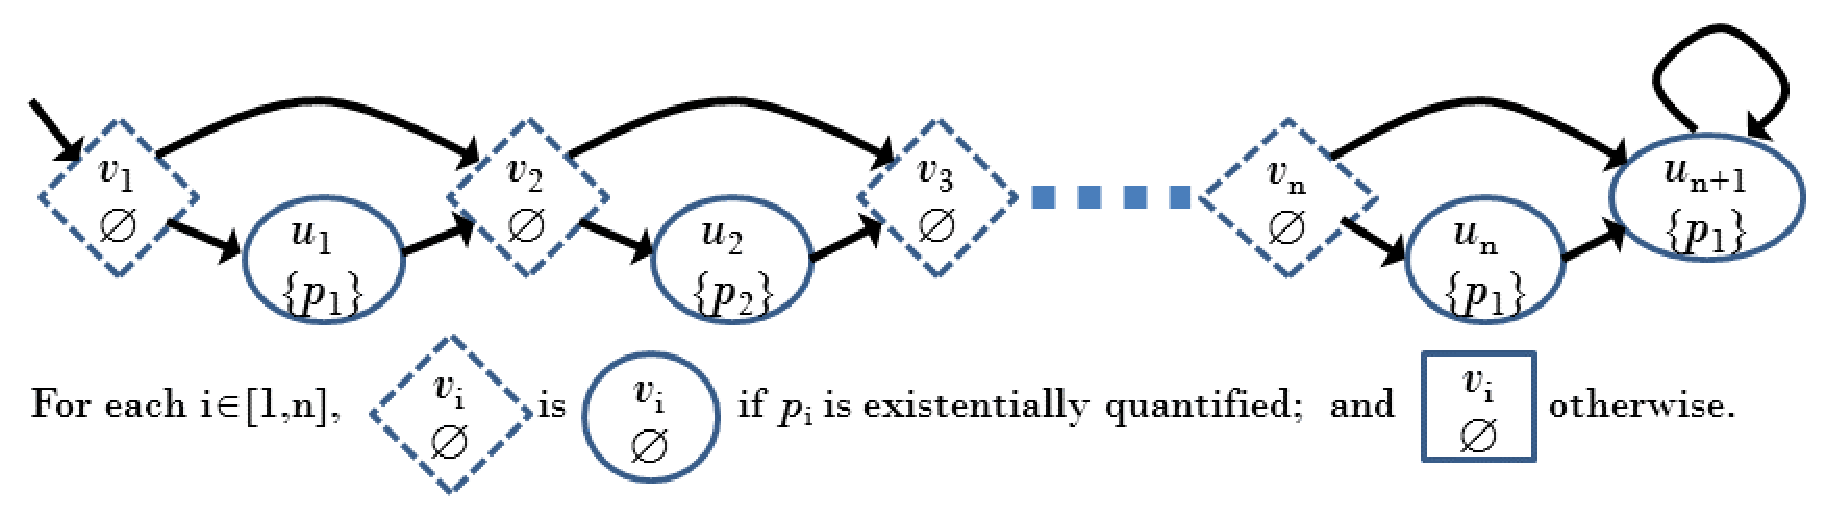
\epsfig{file=gg.altp.eps,width=150mm} 
% \input{gg.atlp.psp80.tex}
\\
$\bigcirc$ belongs to Agent 1 and $\pfrr$ belongs to Agent 2.
\end{center}
\caption{Game graph for the PSPACE-hardness proof of a Boolean formula
with $n$ propositions}
\label{fig.gg.bsil.nphard}
\end{figure}

In the graph, we use oval nodes for states owned by Agent 1 and 
square nodes for states owned by Agent 2.
In each state, we put down its name and the set of atomic
propositions that are true at the node.
For each atomic proposition $p_i\in P$,
we have a corresponding subgraph consisting of nodes
$v_i$ and $u_i$.
The subgraph of $u_i$ corresponds to $\Gamma_{p_i}$ and
and that of $v_i,u_i$ together corresponds to $\Omega_{p_i}$.  

The design of the graph allows only at most one visit
to states $v_1,\ldots,v_n$.
For all $i\in[1,n]$, state $v_i$ is owned by Agent 2 if $p_i$ is
universally quantified;
and owned by Agent 1 otherwise.
If $p_i$ is owned by Agent 1,
then Agent 1 can choose either
$(v_i,u_i)$ or $(v_i,v_{i+1})$.
If $p_i$ is owned by Agent 2,
then both choices of Agent 2 at node $v_i$ must yield
satisfaction of $\eta$.

We construct an ATL$^+$ formula $\phi_\eta$
as % follows.
% \begin{center}
$\langle 1\rangle \bigwedge_{1\leq i\leq k}
\bigvee_{1\leq j\leq h_k} \tau(l_{i,j})$ 
% \end{center}
where $\tau(p)\defn \pevt p$ and $\tau(\neg p)\defn \pfrr \neg p$. 
I.e., $\phi_\eta$ is obtained from $\eta$ by replacing the leading quantifiers in $\eta$ by $\langle 1 \rangle$.

We now show that $\calg_\eta \models \phi_\eta$ if, and only if, $\eta$ is satisfied (i.e., if $\eta$ is a tautology).
The  latter is the case if there is a winning strategy for a `satisfier' in the following game between a `satisfier' and a `refuter':
following the order of the bound variables, the `satisfier' and `refuter' choose the truth value of the existentially and universally bound variables, respectively.
When all variables are assigned truth values, the `satisfier' wins if the CNF formula is satisfied with these values. Otherwise, the refuter wins.

Taking a winning strategy of the satisfier in this game obviously provides a winning strategy for Agent 1 and, vice versa, a winning strategy of Agent 1 in the model-checking game can be used as a winning strategy for the `satisfier' in the satisfaction game.
\qed

We have an example for the reduction in the proof 
of Lemma~\ref{lemma.bsil.mck.nphard}.  

{\example \label{exmp.bsil.nphard}:}
Given
$\eta\equiv \exists p\forall q\exists r
((p\vee q \vee r)\wedge(\neg p \vee \neg r))$,
according to the construction
in the proof of Lemma~\ref{lemma.bsil.mck.nphard},
we have the following ATL$^+$ formula:
$\phi_\eta\defn 
\langle1\rangle(((\pevt p)\vee (\pevt q) \vee (\pevt r))
  \wedge((\pfrr\neg p) \vee (\pfrr\neg r)))$.
\qed

Following Lemmas~\ref{lemma.bsil.mck.nphard} and
\ref{lemma.alg.pspace}, we obtain the complexity of our model-checking problems.

{\lemma\label{lemma.bsil.pspace.complete} The BSIL and ATL$^+$ model-checking
problems are PSPACE-complete.
} \qed



\chapter{Temporal Cooperation Logic}
\label{c:tcl}

\section{TCL}
\subsection{Syntax}
\subsection{semantics}

\section{Expressive Power of TCL}
\subsection{Comparison with CTL* and LTL}
\subsection{Comparison with AMC, ATL* and GL}

\section{Complexity}
\subsection{TCL Model-checking}
\subsection{TCL Satisfiability}

\section{Experiment}

\chapter{Conclusions}
\label{c:conclusions}
%\chapter{Theory of surface plasmon polaritons in metallic nano-structures}
\label{c:thm}
\section{Definition of plasmon}

Plasmon is collective oscillation of conduction electron gas, a quasi-particle resulting from the quantization of plasma oscillations just like phonons are quantizations of mechanical vibrations. The simplest case is the volume plasmon as shown in Figure~\ref{fig:bulk}.
\begin{figure}[htb]
\centering
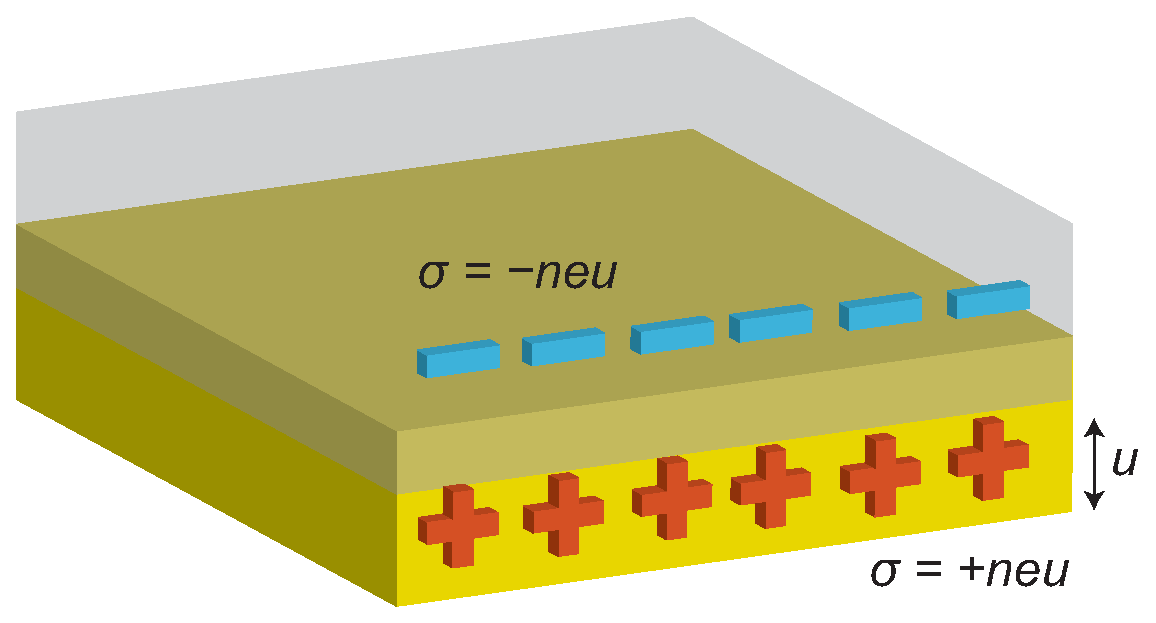
\includegraphics[scale=0.5]{THM/bulk.eps}
\caption{\label{fig:bulk}Longitudinal collective oscillations of the conduction electrons of a metal (Volume plasmons)}
\end{figure}
 We can derive plasma frequency $\omega_p$ from the simple harmonics oscillation model, a collective displacement of the electron cloud by a distance $u$ leads to a surface charge density $\sigma = \pm neu$ at the slab boundaries. This establishes a homogeneous electric field $\mathbf{E} = \frac{neu}{\varepsilon_0}$ inside the slab. Thus, the displaced electrons experience a restoring force, and their movement can be described by the equation of motion $nm\ddot{u} = -ne\mathbf{E}$. Inserting the expression for the electric field, this leads to
 \begin{subequations}
 \begin{align}
 nm\ddot{u} = -\frac{n^2e^2u}{\varepsilon_0} \\
 \ddot{u} + {\omega_p}^{2}u = 0\text{.}
 \end{align}
 \end{subequations}
  The plasma frequency $\omega_p = \sqrt{\frac{ne^2}{\varepsilon_0m}}$ can thus be recognized as the natural frequency of a free oscillation of the electron sea. The quanta of these charge oscillations are called plasmons. Due to the longitudinal nature of the excitation, volume plasmons do not couple to transverse electromagnetic waves, and can only be excited by particle impact. We can derive the dispersion relation of the generalization of volume plasmons, traveling plasma waves, from curl electric field equations (Equations~\ref{eq:curlE})
 \begin{subequations}
 \begin{align}
 \curl{\curl \mathbf{E}} &= -\mu_0 \frac{\partial^2\mathbf{D}}{\partial t^2}\label{eq:curlE}\\
\mathbf{K}( \mathbf{K}\cdot \mathbf{E}-K^{ 2 }\mathbf{E} ) &=-\varepsilon ( \mathbf{K},\omega  ) \frac { { \omega  }^{ 2 } }{ { c }^{ 2 } } \mathbf{E}
 \end{align}
 \end{subequations}  
and plasma model, and a simple equation of motion for an electron of the plasma subjected to an external electric field $\mathbf{E}$
 \begin{equation}
m\ddot{\mathbf{x}} + m\gamma\dot{\mathbf{x}} = -e\mathbf{E}\text{.}
\end{equation}
Assuming a harmonic time dependence $\mathbf{E}( t )=\mathbf{E}_0\mathrm{e}^{-i\omega t}$ of the driving field, a particular solution of this equation describing the oscillation of the electron is $\mathbf{x} ( t ) = \mathbf{x}_0 \mathrm{e}^{-i\omega t} $. The complex amplitude $\mathbf{x}_0$ incorporates any phase shifts between driving field and response via
\begin{equation}
\mathbf{x} ( t ) = \frac{e}{m( \omega^2 + i\gamma\omega )}\mathbf{E}( t )\text{.}
\end{equation}
The displaced electrons contribute to the macroscopic polarization
\begin{equation}
\mathbf{P}=-\frac{ne^2}{m( \omega^2 + i\gamma\omega )}\mathbf{E}( t )\text{.}
\end{equation}
Inserting $\mathbf{P}$ into dielectric displacement field equation $\mathbf{D} = \varepsilon_0\mathbf{E} + \mathbf{P}$ yields
\begin{equation}
\mathbf{D} = \varepsilon_0(1-\frac{\omega_p^2}{\omega^2 + i\gamma\omega})\mathbf{E}\text{,}
\end{equation}
where $\omega_p^2 = \frac{ne^2}{\varepsilon_0m}$. Therefore, the dielectric function of the free electron gas
\begin{equation}
\varepsilon(\omega) = 1- \frac{\omega_p^2}{\omega^2 + i\gamma\omega}\text{.}\label{eq:dielefu}
\end{equation}
We arrive at the desired result by using equation~\ref{eq:dielefu} and the generic dispersion relation $K^2=\varepsilon(\mathbf{K},\omega)\frac{\omega^2}{c^2}$, the dispersion relation of traveling waves becomes
\begin{equation}
\omega^2 = \omega_p^2 + \mathbf{K}^2c^2\text{.}
\end{equation}
From this relation, we can figure out the oscillation properties in any frequency of external field. Note that this branch can not confine the electromagnetic waves, it would radiate out the energy, so this mode is also called radiative surface plasmon.

\section{Surface plasmon polaritons at interface between dielectric and metal}

Surface plasmon polaritons (SPPs) are eigenmodes of transverse magnetic (TM) waves, which coupling the electromagnetic fields to oscillations of the conductor's electron plasma, propagate at a interface between dielectric and metal, and are confined in perpendicular direction. Providing a flat interface between dielectric and metal half-spaces with dielectric constants $\varepsilon_d$ and $\varepsilon_m$ , respectively, and assuming the interface normal to z direction and the SPPs propagate along the $x$ direction, the SPP wave vector $\beta$ is related to the frequency $\omega$ through the dispersion relation
\begin{equation}
\beta = k_0\sqrt{\frac{\varepsilon_d\varepsilon_m}{\varepsilon_d + \varepsilon_m}}\text{,}\label{eq:sppsdisp}
\end{equation}
where $k_0 = \omega/c$ is the free-space wave vector. We take $\omega$ to be real and allow $\beta$ to be complex.

The optical response of metals is often described by the Drude model for a free-electron gas~\cite{kittel1976introduction},
\begin{equation}
\varepsilon_{Drude}(\omega)=1-\frac{\omega_p^2}{\omega^2+i\Gamma\omega}\text{,}
\end{equation}
in which $\Gamma$ is a damping rate due to electron-electron and electron-phonon scattering.
Figure~\ref{fig:SPPdisp} shows the dispersion curve~\ref{eq:sppsdisp} with Drude metal  in the absence of losses ($\Gamma=0$) for air ($\varepsilon_d = 1$) and fused silica ($\varepsilon_d = 2.25$) interface.
\begin{figure}[htb]
\centering
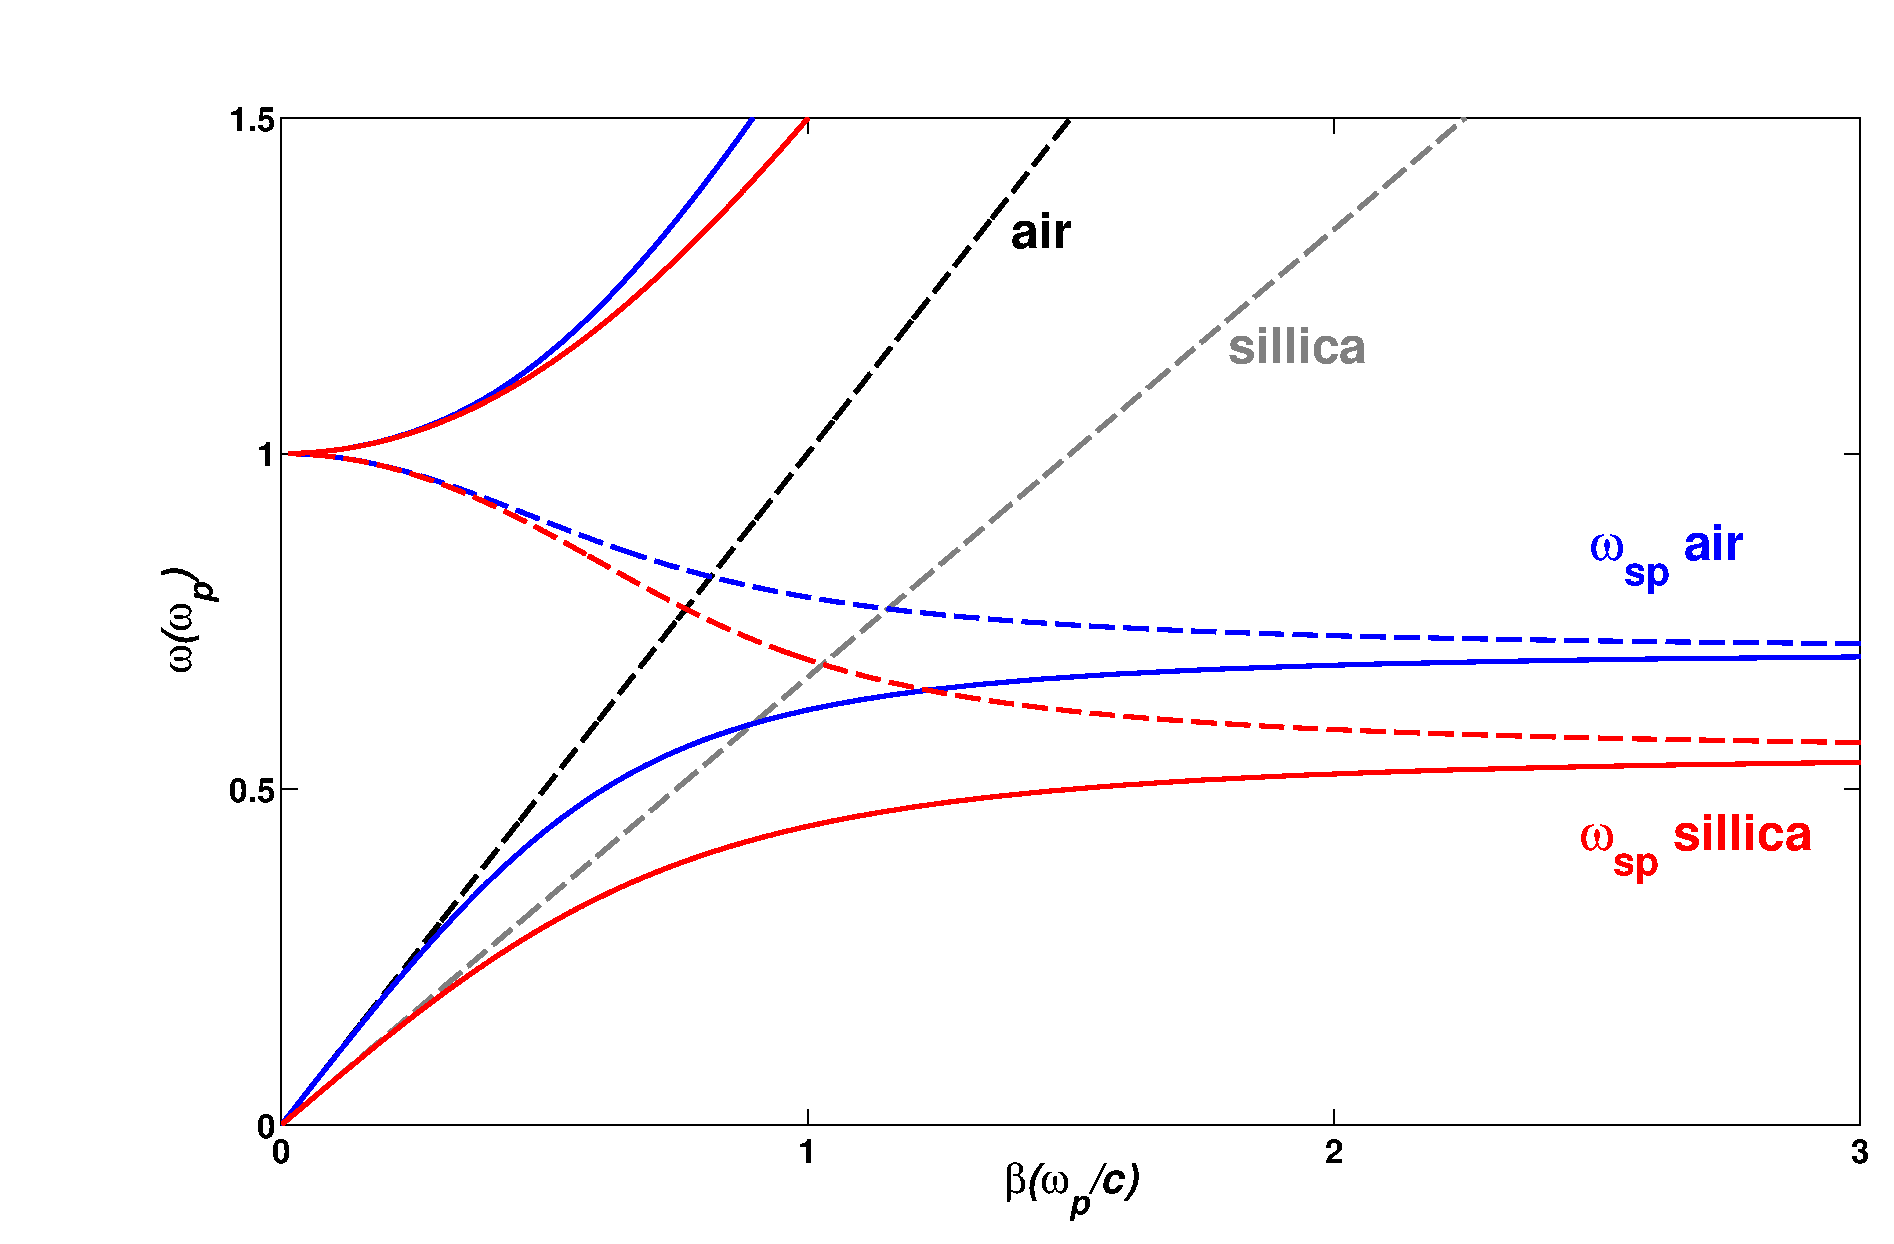
\includegraphics[scale=0.4]{THM/SPPdisp.eps}
\caption{\label{fig:SPPdisp}Dispersion relation of SPPs at the interface between a Drude metal with negligible collision frequency and air (blue curves) and silica (red curves).}
\end{figure}
For small wave vectors SPPs propagation constant $\beta$ is close to $k_0$ at the light line, in the opposite regime of the frequency close to surface plasmon frequency $\omega_p$. It also shows that the SPPs line lying to the right of the respective light lines of air and silica, so that SPPs are directed by light due to phase mismatching. The wave vector mismatch between SPPs and radiation modes needs to be overcome in order to excite or detect SPPs. This can be achieved by multiple methods~\cite{raether1988surface}. In the Otto configuration, light in a prism that is brought in close vicinity to a metal surface can excite SPPs through coupling to the evanescent field. Because light in the prism has a larger wave vector than that in air, it can be phase-matched to the SPPs. In the related Kretschmann-Raether geometry, coupling to SPPs occurs through a metal film that is deposited on a prism. In the grating coupling configuration, metal surface with a shallow grating of grooves or holes with lattice constant $a$. For the simple 1D grating of grooves depicted in Figure~\ref{fig:grating},
\begin{figure}[htb]
\centering
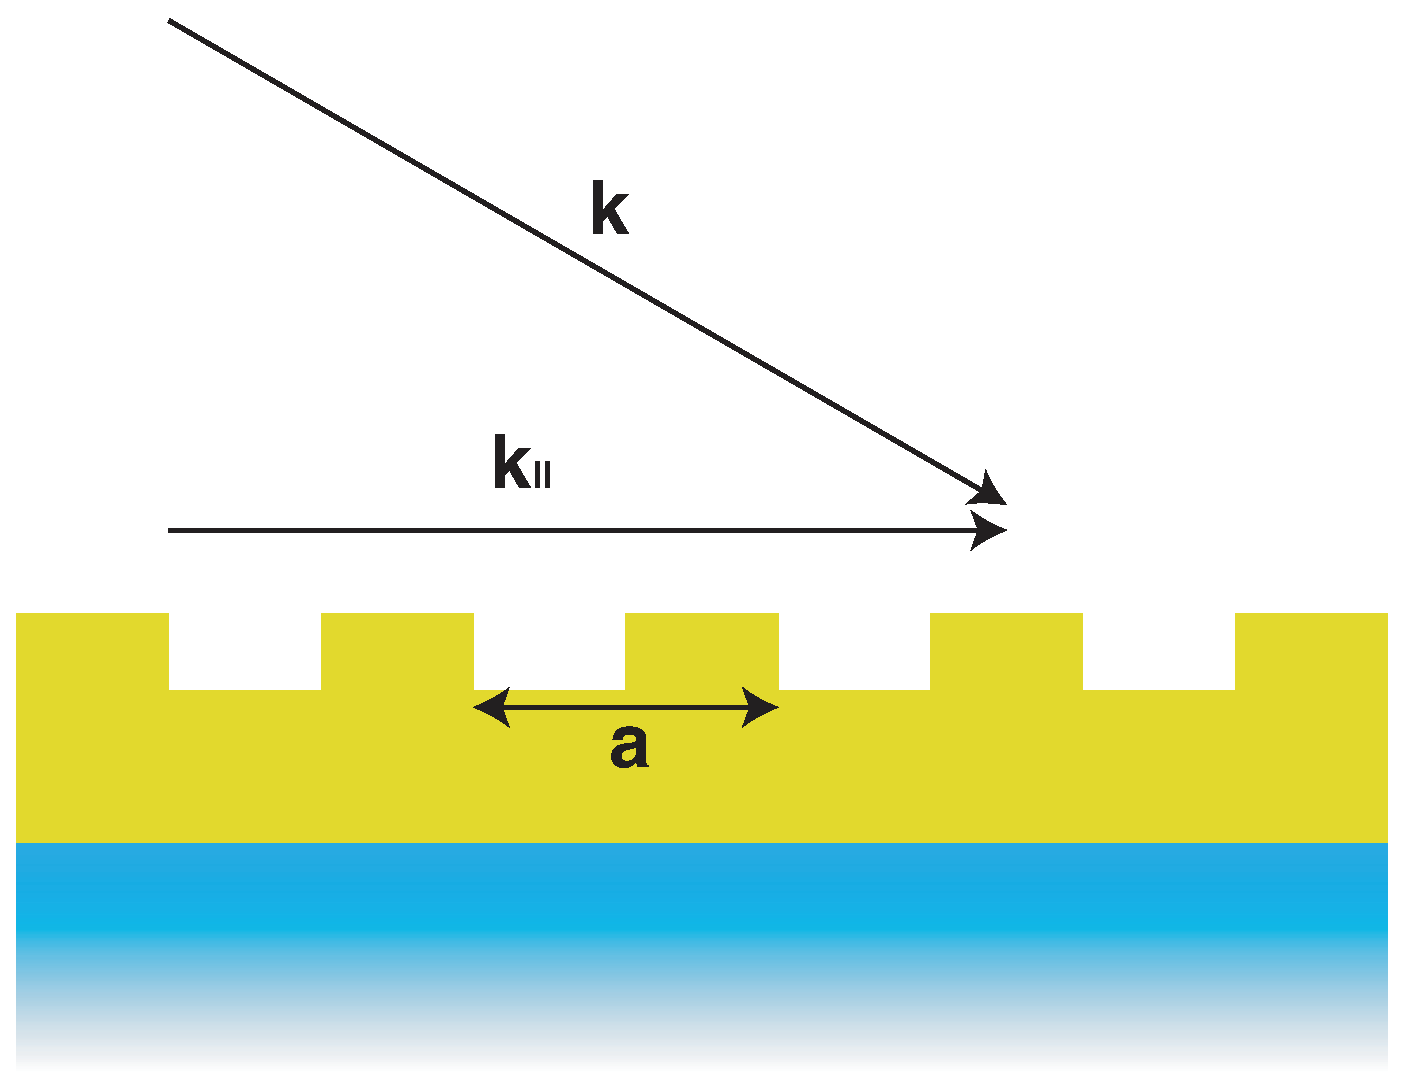
\includegraphics[scale=0.5]{THM/grating.eps}
\caption{\label{fig:grating}Phase-matching of light to SPPs the grating coupling configuration.}
\end{figure}
phase-matching takes place when the condition is fulfilled
\begin{equation}
\beta = k_0 \sin{\theta} \pm \nu g\text{,}
\end{equation}
where $g=\frac{2\pi}{a}$ is the reciprocal vector of the grating, and $\nu=(1,2,3\dots)$.
As with prism coupling, excitation of SPPs is detected as a minimum in the reflected light. The reverse process can also take place, SPPs propagating along a surface modulated with a grating can couple to light and thus radiate. 

%\bibliographystyle{unsrt}
%\bibliography{thesisbib}
%\chapter{Experiment}
\label{c:exp}

\section{Atomic force microscopy}

\begin{figure}[htb]
\centering
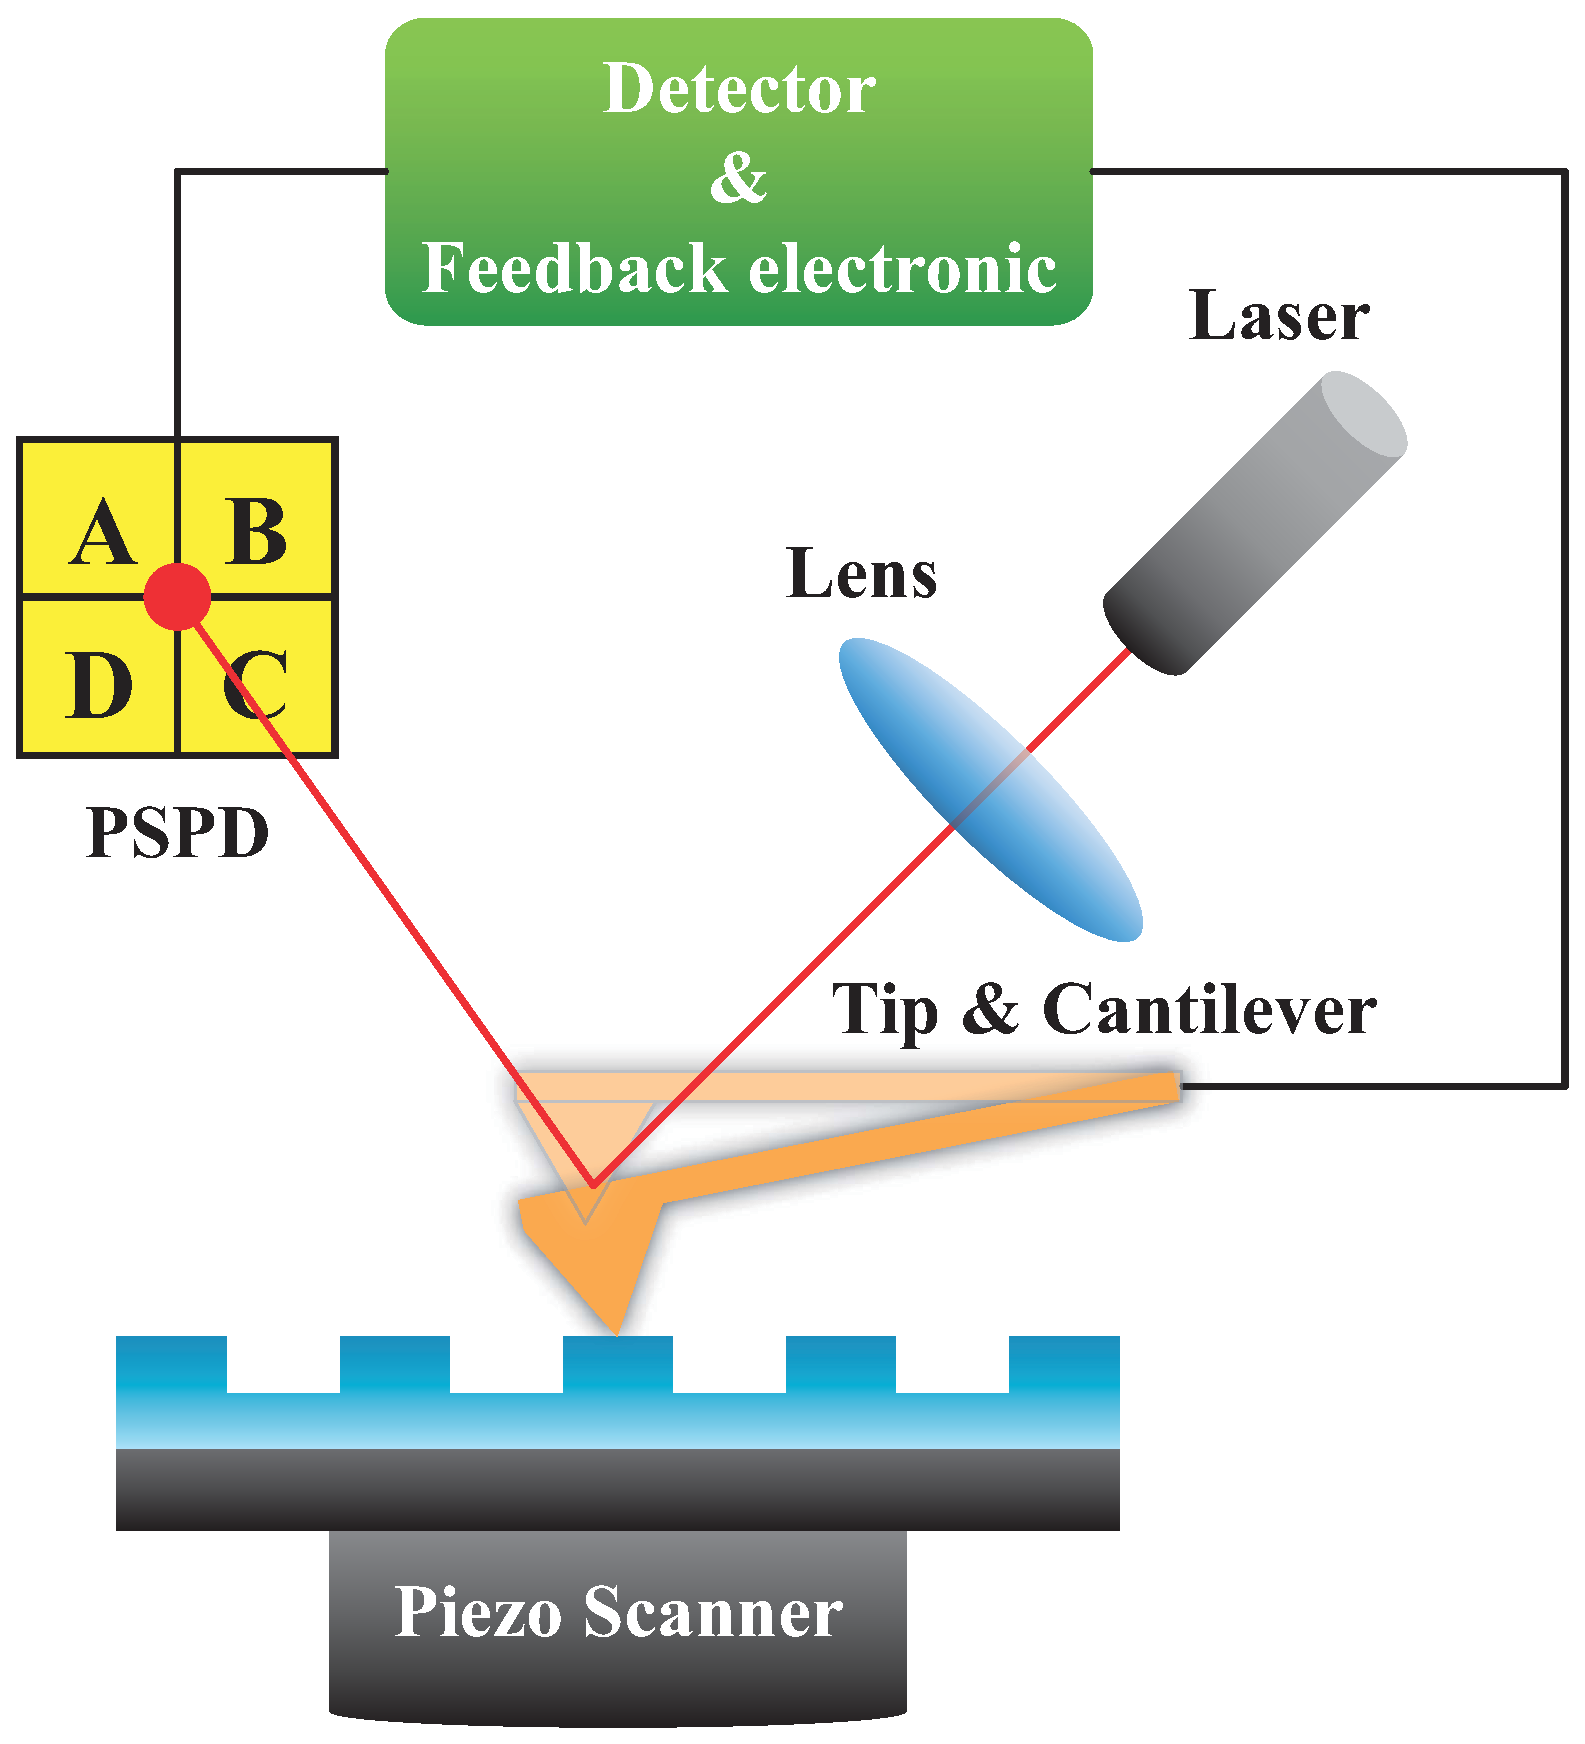
\includegraphics[scale=0.35]{EXP/afm1.eps}
\caption{\label{fig:afm1}Schematic of atomic force microscopy.}
\end{figure}
Atomic force microscope (AFM) is a type of scanning probe microscopes (SPM)~\cite{bennig1988atomic}.  The schematic of AFM is shown in Figure~\ref{fig:afm1}. AFM operates by measuring force between a probe and the specimen surfaces. In general,  the probe is a sharp tip at a cantilever's end. The cantilever can be deflected by atomic forces to sufficiently large amount, then AFM can measure the vertical and lateral deflections of the cantilever by using the optical system. A laser beam is transmitted to cantilever, and the reflected laser beam is detected with a position-sensitive photo detector (PSPD). PSPD is four-sectional that allows measuring not only vertical but lateral bending too(Figure~\ref{fig:afm2}). The output of the PSPD is provided to a computer for processing of the data for providing a topographical image of the surface with atomic resolution, and controlling the height between probe and specimen surfaces by applying voltage on piezoelectric scanner.
\begin{figure}[htb]
\centering
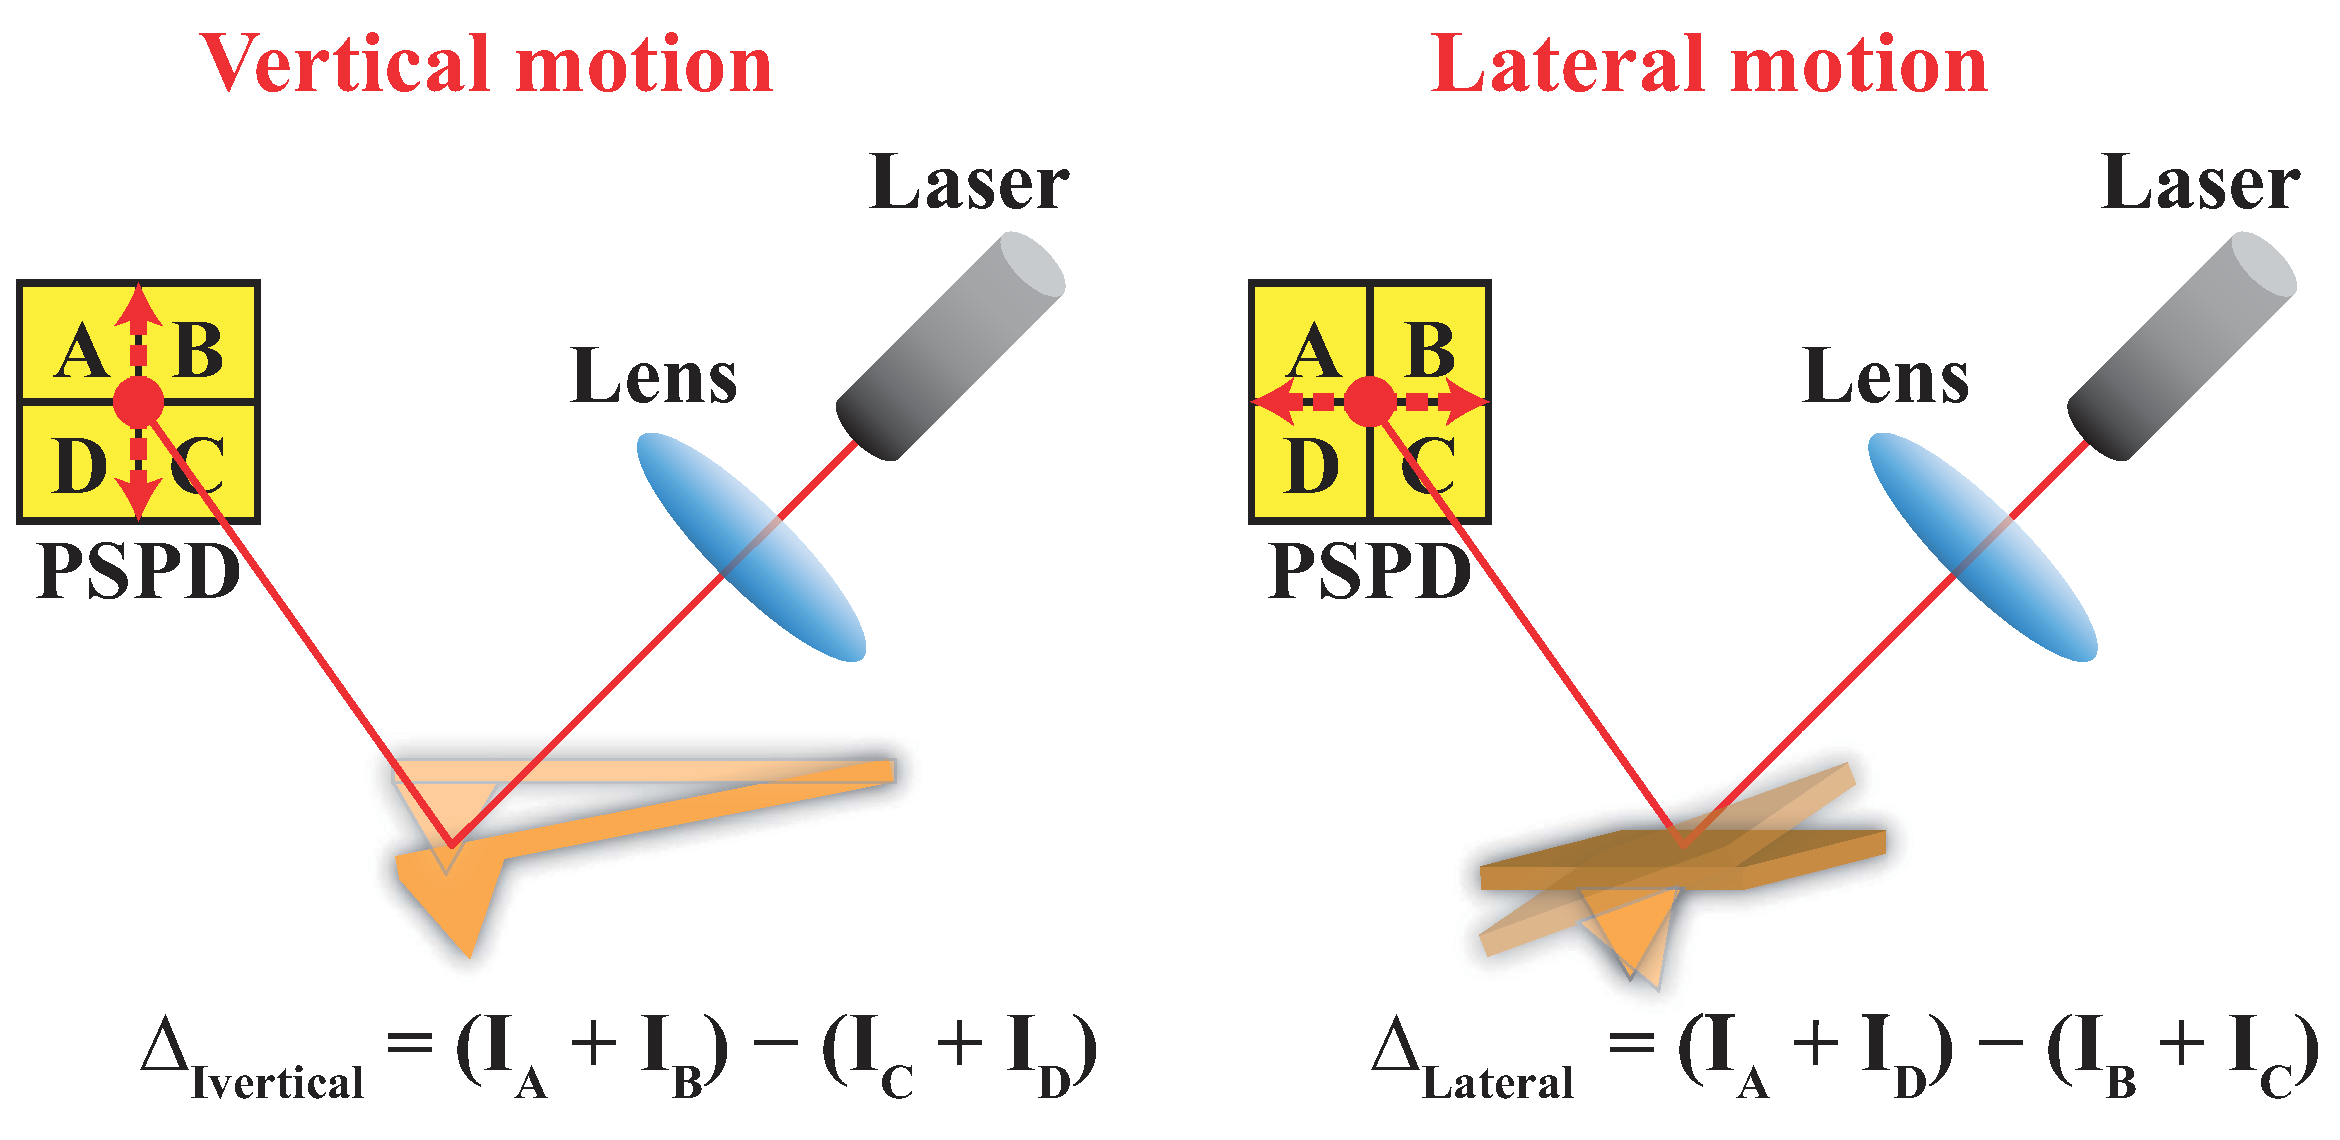
\includegraphics[scale=0.4]{EXP/afm2.eps}
\caption{\label{fig:afm2}Schematic of optical system for cantilever deflections detection.}
\end{figure}

The physical principle of the AFM operation is based on interaction between the probe tip and the specimen surface(Figure~\ref{fig:afm3}). When the cantilever approaches the specimen surface, Van der Waals forces start acting upon it . They are sufficiently far-ranging and are felt at the distance of a few tens of angstroms. Then at the distance of several angstroms repulsive force starts acting. In humid air a water layer is present on the specimen surface. The capillary force arises that holds the tip in contact with the surface and increases the minimum achievable interaction force. Electrostatic interaction between the probe and the sample may appear rather often. This can be both attraction and repulsion. Van der Waals attraction forces, capillary, electrostatic and repulsion forces at the point where the tip touches the sample and forces acting upon the tip from the deformed cantilever compensate each other in equilibrium. Based on the type and degree of this interaction the AFM modes can be broken down into contact and semi-contact(Figure~\ref{fig:afm3} ), which is a transition mode between the contact and non-contact modes.
\begin{figure}[htb]
\centering
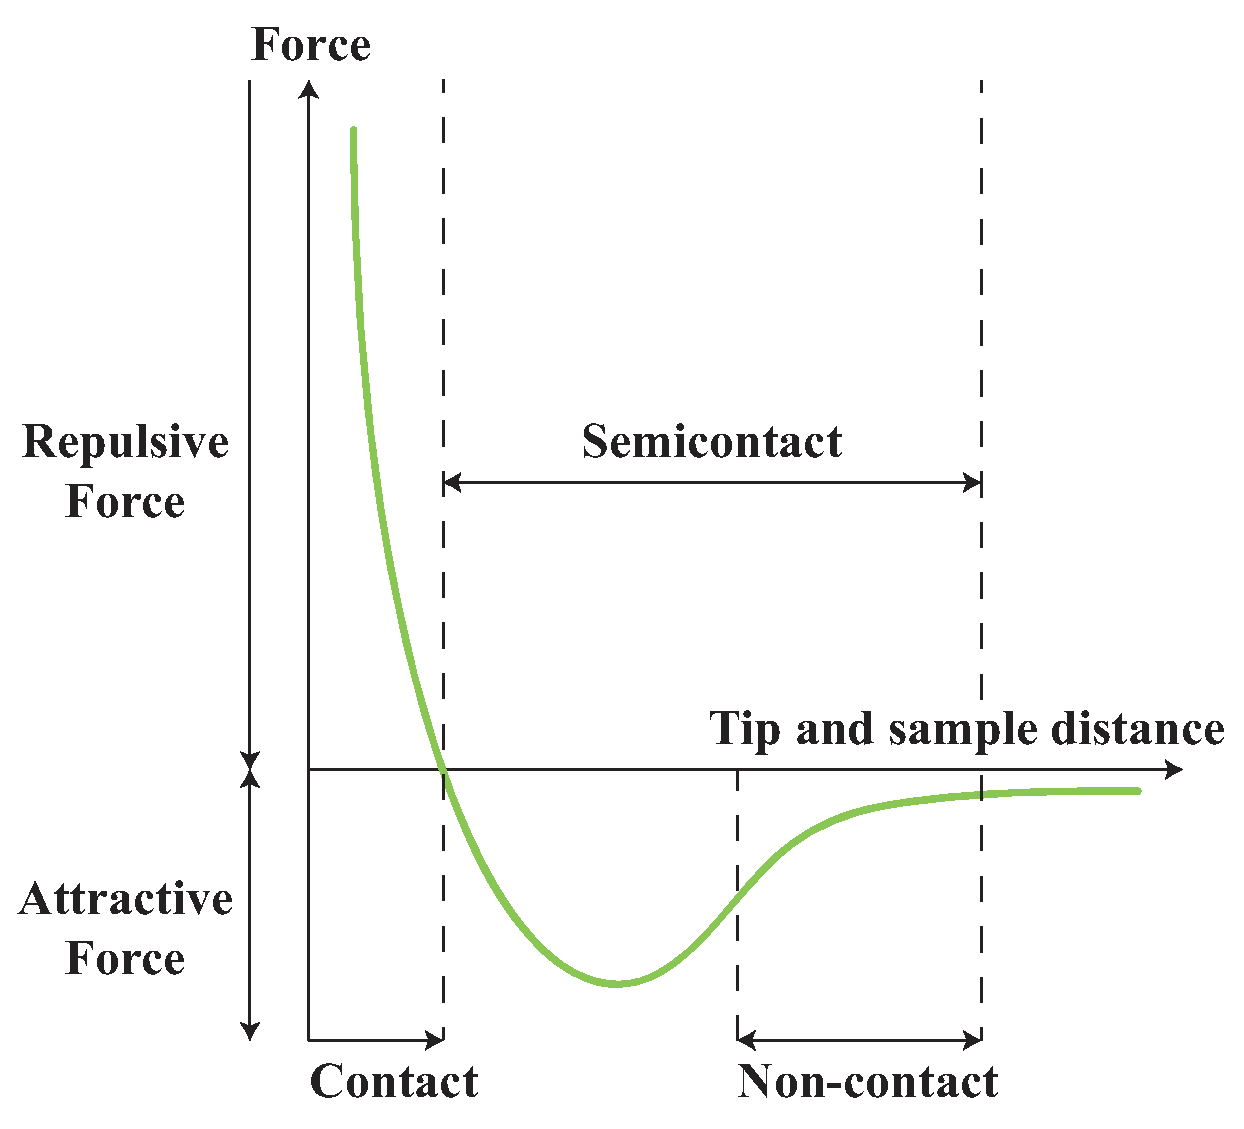
\includegraphics[scale=0.6]{EXP/afm3.eps}
\caption{\label{fig:afm3}Sketch of tip-sample forces.}
\end{figure}

\paragraph{Contact mode}

In contact mode of operation the cantilever deflection under scanning reflects repulsive force acting upon the tip. Repulsion force $\mathbf{F}$ acting upon the tip is related to the cantilever deflection value $\mathbf{x}$ under Hooke's law: $\mathbf{F}=-K \cdot  \mathbf{x}$, where $K$ is cantilever spring constant. The spring constant values for different cantilevers usually vary from 0.01 to several $\mathbf{N/m}$.

In our units the vertical cantilever deflection value is measured by means of the optical registration system and converted into electrical signal DFL (difference signal between the upper and lower halves of the PSPD) . In contact mode the DFL signal is used as a parameter characterizing the interaction force between the tip and the surface. There is a linear relationship between the DFL value and the force. In constant force mode of operation the deflection of the cantilever is maintained by the feedback circuitry on the preset value. So vertical displacement of the scanner under scanning reflects topography of sample under investigation.

Contact force microscopy is surface topography measurement in the contact mode.The microscope operation in the mode of maintaining constant interaction force between the tip and the surface sample, and is the base for measuring surface topography as well as for measuring local rigidity, local viscosity and local friction force. Constant force mode has some advantages and disadvantages. Main advantage of constant force mode is possible to measure with high resolution simultaneously with topography and some other characteristics, such as friction forces, spreading resistance etc. Constant force mode has also some disadvantages. Speed of scanning is restricted by the response time of feedback system. When exploring soft samples they can be destroyed by the scratching because the probe scanning tip is in direct contact with the surface. Therefore, under scanning soft unhomogeneous samples the local flexure of sample surface varies. As a result acquired topography of the sample can be proved distorted. Possible existence of substantial capillary forces imposed by a liquid adsorption layer can decrease the resolution.

\paragraph{Semi-contact mode}

The semi-contac mode can be characterized by some advantages in comparison with contact mode. First of all, in this mode the force of pressure of the cantilever onto the surface is less, that allows to work with softer materials such as polymers and bio-organics. The semi contact mode is also more sensitive to the interaction with the surface that gives a possibility to investigate some characteristics of the surface distribution of magnetic and electric domains, elasticity and viscosity of the surface. 

Widely used semi-contact mode has some disadvantage concerned with the usage of the feedback circuit. The scanning speed in semi-contact mode is restricted by the feedback circuit reaction time. This disadvantage can be overcome by the fact that under scanning new value of cantilever oscillation amplitude (and error signal) usually is achieved faster than preset value of the cantilever oscillation amplitude can be reached by the feedback system. Time of the reaching new value of the oscillation amplitude is determined by the oscillation period and Q-quality of the cantilever.
The feedback error signal, emerging when scanning in the semi-contact mode, contains some additional information about the topography. It can be utilized for achieving a more precise recovery of the relief. 

Additionally, similarly to the contact error mode, which can be considered as intermediate between the constant force mode and constant height mode, the feedback gain factor (i.e. the feedback processing speed) can be adjusted for the system to be able to trace subtle changes of the relief and to be too slow to trace the steep changes. Then, when the probe travels over minor irregularities, scanning will be carried out with an almost constant piezo scanner length. As a result, the slow changes of the relief will hardly show up on the images, and the steep changes will appear in high contrast. This may be helpful in finding minor irregularities on large areas against major sloping relief features. It must be noted that height of the minor irregularities must be less than amplitude of cantilever oscillation.

\section{Scanning electron microscopy}

The scanning electron microscope (SEM) is used for the observation of specimen surfaces~\cite{von1938elektronen}. When the specimen is irradiated with a fine electron beam, secondary electrons are emitted from the specimen surface. Topography of the surface can be observed by two-dimensional scanning of the electron probe over the surface and acquisition of an image from the detected secondary electrons. The concept schematic of commercial SEM (JEOL, JSM-6500F) is shown in Figure~\ref{fig:sem1}. The basic unit is composed of an electron optical system, a specimen stage, a secondary-electron detector, an image display unit, and an operation system. The electron optical system consists of an electron gun, a condenser lens and an objective lens to produce an electron probe, a scanning coil to scan the electron probe, and other components. The system inside of the microscope column are kept at vacuum.
\begin{figure}[htb]
\centering
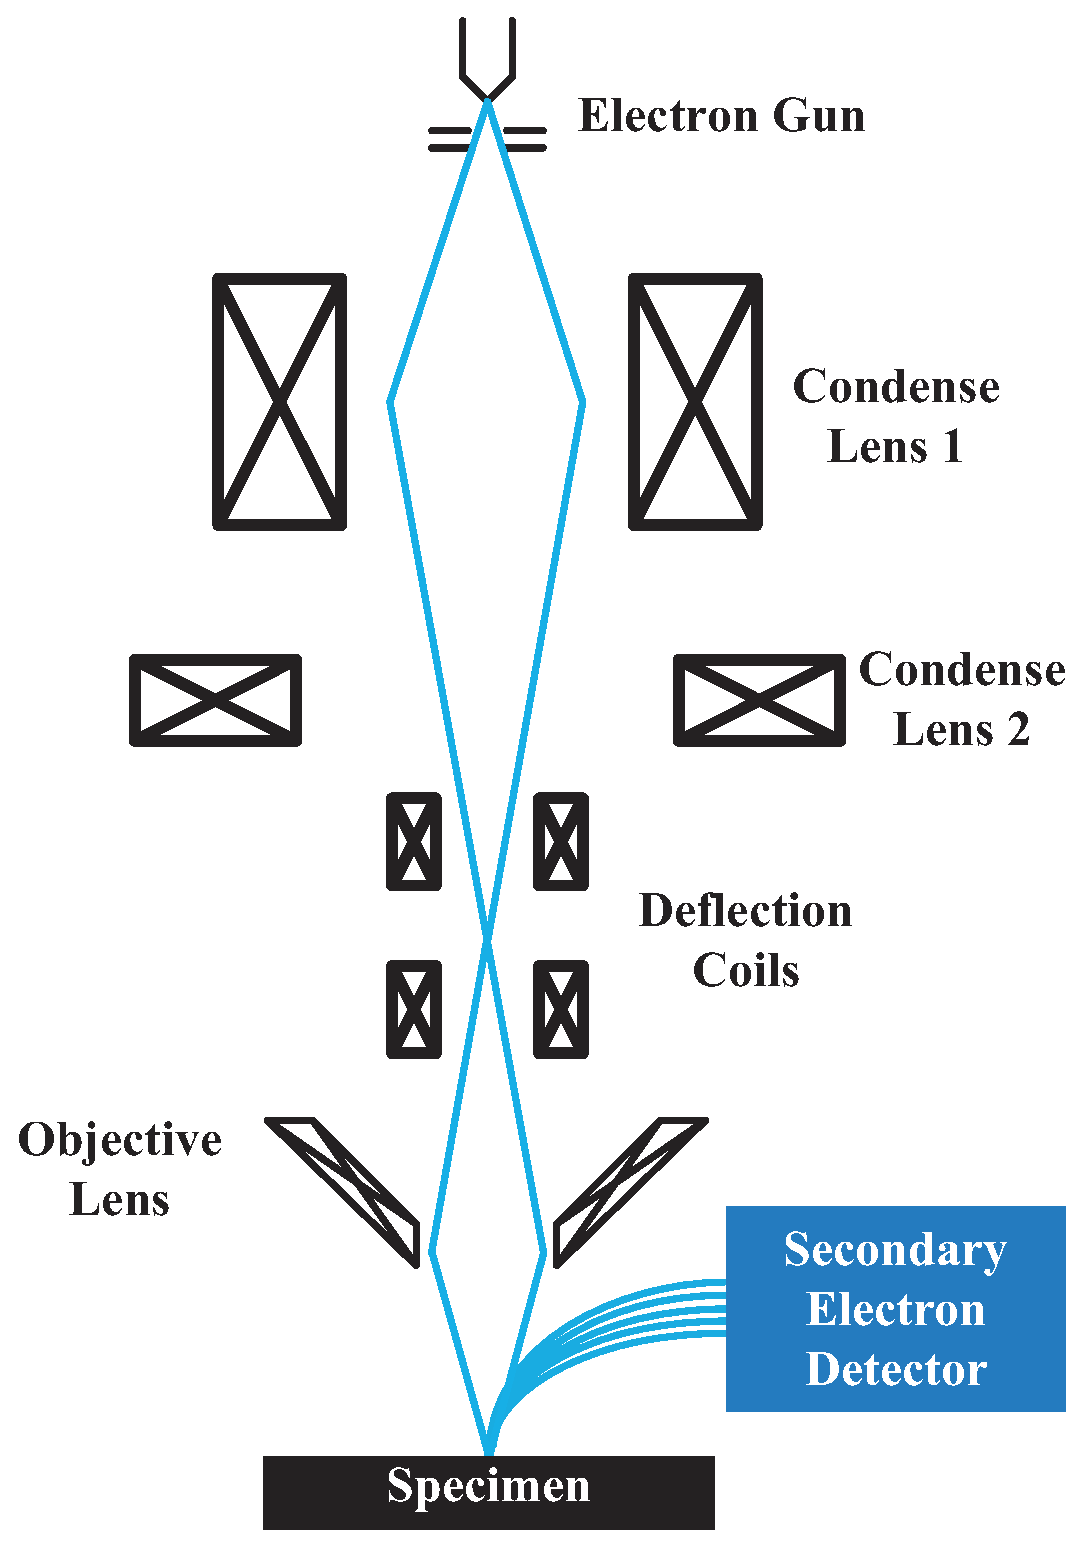
\includegraphics[scale=0.5]{EXP/SEM.eps}
\caption{\label{fig:sem1}Basic construction of a scanning electron microscopy.}
\end{figure}


The JSM-6500F utilizes a Schottky type field-emission (T-FE) gun for the electron source. The T-FE gun can constantly supply the surface of the cathode with zirconium oxide by heating the surface of cathode to 1800 K. For this reason, it can easily obtain stable and high probe current (range from several pA to 100 nA) compared with the traditional thermal emission electron gun and cold field-emission gun.

The magnetic condenser and objective lens system act to control the diameter of the beam as well as to focus the beam on the specimen due to a rotationally-symmetric magnetic field is formed when we pass a direct electric current through a coilwound electric wire in the magnetic lens. A pair of deflector coils, which between the condenser and objective lens, controlled by the scan generator, which are responsible for rastering that focused beam across the specimen surface. The size of the rastering pattern is under magnification control. The beam is rastered from left to right and top to bottom. There is a one-to-one correspondence between the rastering pattern on the specimen and the rastering pattern used to produce the image on the monitor. The resolution we choose to image at will obviously affect the number of pixels per row as well as the number of rows that constitute the scanned area.

The signal is generated from the specimen, and collected by the detector and subsequently processed to generate the image. That processing takes the intensity of the signal coming from a pixel on the specimen and converts it to a grayscale value of the corresponding monitor pixel. The monitor image is a two dimensional rastered pattern of grayscale values.

With the beam focused on the specimen surface, all we need to do to change magnification is to change the size of the rastered area on the specimen. The size of the monitor raster pattern is constant. Magnification will increase if we reduce the size of the area scanned on the specimen.

%\bibliographystyle{unsrt}
%\bibliography{thesisbib}
%\input{main}

%chapter cite  == \include

%\chapter{Get started with \LaTeX\ }
\label{c:GetStarted}
Two common font styles in this text: 
\begin{itemize}
    \item \textbf{Item1}: \textit{Italic}     
    \item \textbf{Item2}: \textbf{Bold}
\end{itemize}

About the advance latex grammer see the next section \ref{s:AdvancedFeatures}.


\section{\LaTeX\ Adavanced Features}
\label{s:AdvancedFeatures}
The following features would be introduced in the coming subsections:
\begin{itemize}
    \item SubSection \ref{ss:Figure}: \hyperref[ss:Figure]{\textbf{Figure}}
    \item SubSection \ref{ss:VerbUsage}: \hyperref[ss:VerbUsage]{\textbf{Verb}}
    \item SubSection \ref{ss:VerbUsage}: \hyperref[ss:VerbUsage]{\textbf{Verb}}
    \item SubSection \ref{ss:Enumeration}: \hyperref[ss:Enumeration]{\textbf{Enumeration}}
    \item SubSection \ref{ss:Table}: \hyperref[ss:Table]{\textbf{Table}}
    \item SubSection \ref{ss:CodeDisplay}: \hyperref[ss:CodeDisplay]{\textbf{Code Display}}
    \item SubSection \ref{ss:Math}: \hyperref[ss:Math]{\textbf{Math}}
    \item SubSection \ref{ss:Algorithms}: \hyperref[ss:Algorithms]{\textbf{Algorithms}}
\end{itemize}

%==========================================================================================
\subsection{Figure}
\label{ss:Figure}
\begin{figure}[htpb!]
  \centering
    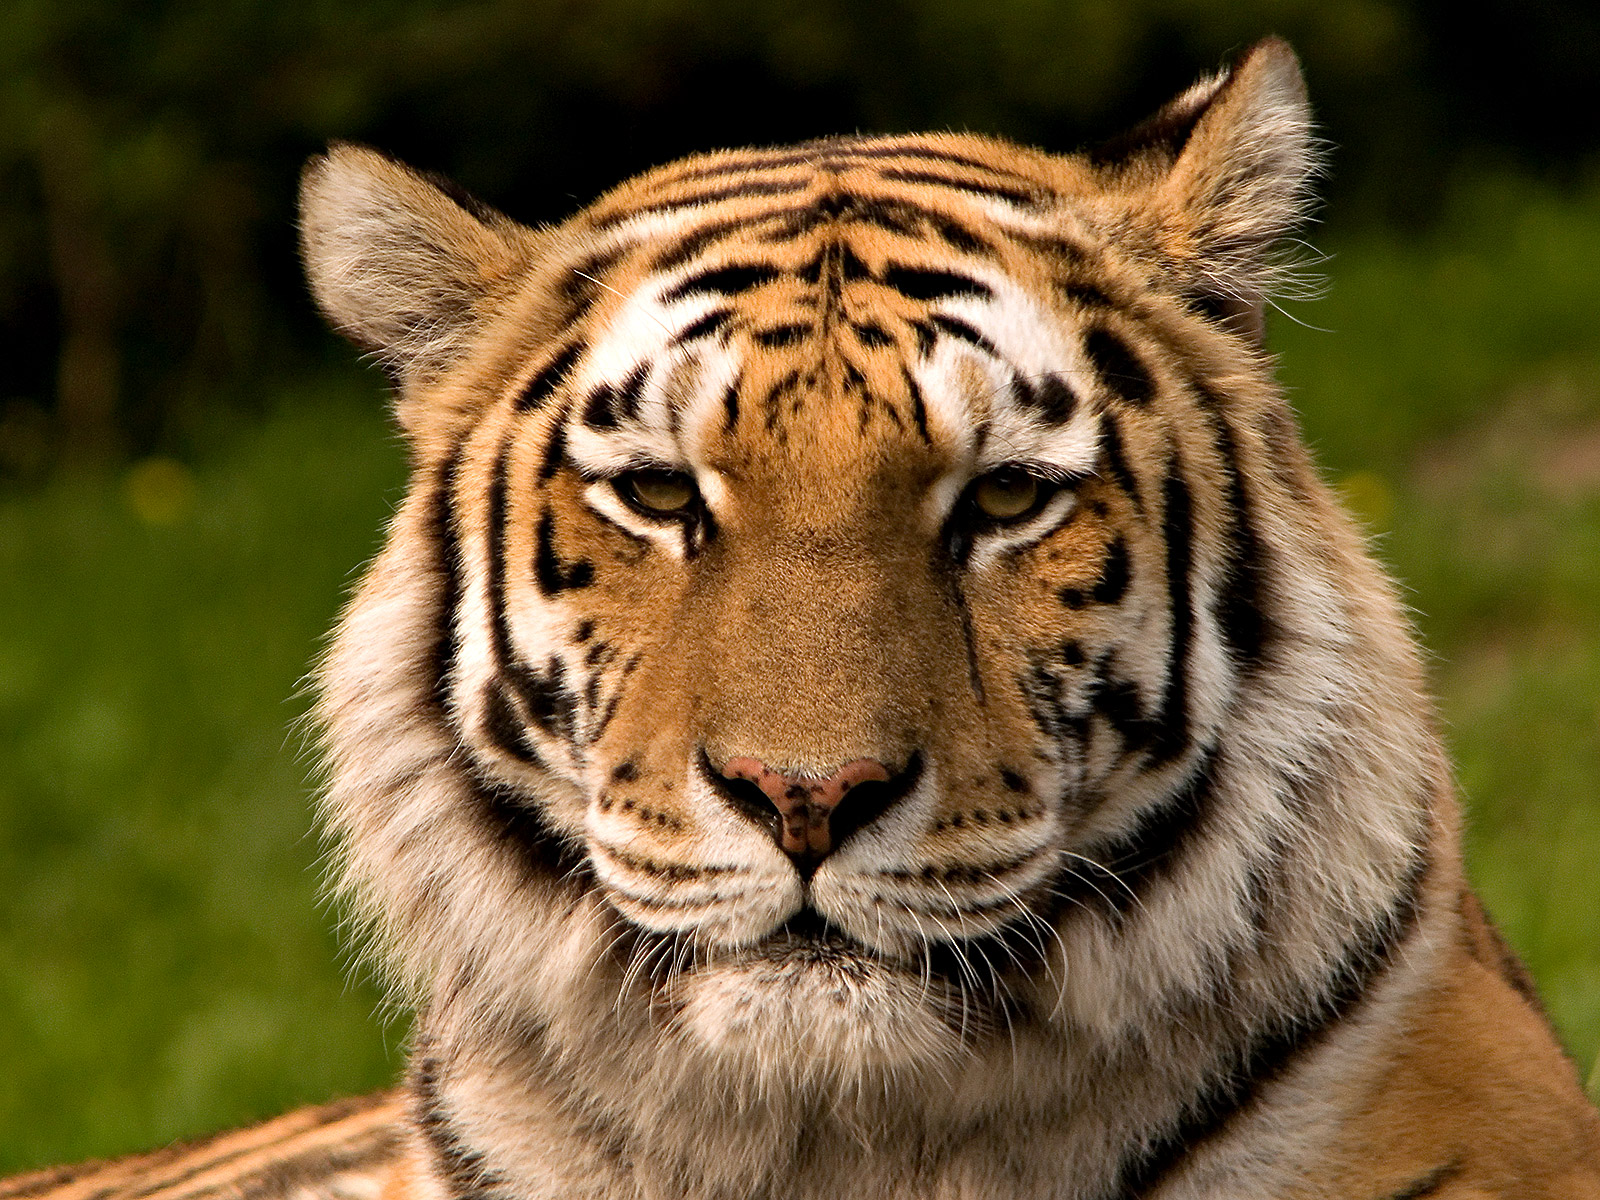
\includegraphics[width=0.5\textwidth]{fig/tiger.jpeg}
    \caption{\label{fig:tiger}A picture of a tiger.}
\end{figure}

Figure~\ref{fig:tiger} is a picture of a tiger.


%==========================================================================================
\subsection{Table}
\label{ss:Table}

\href{http://en.wikibooks.org/wiki/LaTeX/Tables}{Table examples on WIKIBOOKS}.

\begin{table}[htpb]\begin{center}
\caption{Table Example 1}
\begin{tabularx}{8cm}{llX}
\hline
Start & End  & Character Block Name \\
\hline
3400  & 4DB5 & CJK Unified Ideographs Extension A \\
4E00  & 9FFF & CJK Unified Ideographs \\
\hline
\end{tabularx}
 \end{center}\end{table}

\begin{table}[htpb]\begin{center}
\caption{Table Example 2}
\begin{tabular}{llr}
\hline
\multicolumn{2}{c}{Item} \\
\cline{1-2}
Animal & Description & Price (\$) \\
\hline
Gnat  & per gram & 13.65 \\
      & each     &  0.01 \\
Gnu   & stuffed  & 92.50 \\
Emu   & stuffed  & 33.33 \\
Armadillo & frozen & 8.99 \\
\hline
\end{tabular}
 \end{center}\end{table}
 
 \begin{table}[htpb]\begin{center}
	\label{t:prefix-table}
	\caption{Table Example 3}
	\renewcommand{\arraystretch}{1.0}
	\begin{tabularx}{300pt}{|c|X| }
		\hline
		\multirow{1}{*}{\textbf{Allocation}} &
		Allocation, Element, Type, Script 
		\\ \hline\hline
		%------------------------------
		\multirow{6}{*}{\textbf{Data Types}} &
        Byte2, Byte3, and Byte4\\ &
        Float2, Float3, Float4\\ &
        Int2, Int3, Int4\\ &
        Long2, Long3, Long4\\ &
        Matrix2f, Matrix3f, Matrix4f\\ &
        Short2, Short3, Short4
        \\ \hline\hline
		%------------------------------
		\multirow{4}{*}{\textbf{Graphics}} &
		Mesh\\&
		ProgramFragment, ProgramRaster\\&
		ProgramStore, ProgramVertex\\&
		RSSurfaceView
		\\ \hline
		%------------------------------
	\end{tabularx}
\end{center}\end{table}

\begin{table}[htpb]\begin{center}
\caption{Table Example 4}
\begin{tabular}{|l|l|l|}
\hline
\multicolumn{3}{|c|}{Team sheet} \\
\hline
Goalkeeper & GK & Paul Robinson \\ \hline
\multirow{4}{*}{Defenders} & LB & Lucus Radebe \\
 & DC & Michael Duberry \\
 & DC & Dominic Matteo \\
 & RB & Didier Domi \\ \hline
\multirow{3}{*}{Midfielders} & MC & David Batty \\
 & MC & Eirik Bakke \\
 & MC & Jody Morris \\ \hline
Forward & FW & Jamie McMaster \\ \hline
\multirow{2}{*}{Strikers} & ST & Alan Smith \\
 & ST & Mark Viduka \\
\hline
\end{tabular}
 \end{center}\end{table}
 
 \begin{table}[htpb]\begin{center}
\caption{Table Example 5}
 \begin{tabular}{l*{6}{c}r}
Team              & P & W & D & L & F  & A & Pts \\
\hline
Manchester United & 6 & 4 & 0 & 2 & 10 & 5 & 12  \\
Celtic            & 6 & 3 & 0 & 3 &  8 & 9 &  9  \\
Benfica           & 6 & 2 & 1 & 3 &  7 & 8 &  7  \\
FC Copenhagen     & 6 & 2 & 1 & 2 &  5 & 8 &  7  \\
\end{tabular}
 \end{center}\end{table}

%==========================================================================================
\subsection{Verb}
\label{ss:VerbUsage}
Let's take a overview on how to type special characters:\\
\verb|<FRAMEWORKS_BASE>/graphics/java/android/renderscript|\\\footnote{Path of <APP\_intermediates>: <ANDROID\_ROOT>/out/target/common/obj/APPS/APPNAME\_intermediates/}
You could also go back to the beginning of the chapter by the \hyperref[c:GetStarted]{\textbf{hyperref}}.

%==========================================================================================
\subsection{Enumeration}
\label{ss:Enumeration}
\begin{enumerate}
\item Enumerated Item1
\item Enumerated Item2
\item Enumerated Item3
\end{enumerate}

%==========================================================================================
\subsection{Code Display}
\label{ss:CodeDisplay}

\lstset{
	language=C++,
	stringstyle=\rmfamily,
	commentstyle=\itshape\color[rgb]{0.133,0.545,0.133},
	showstringspaces=false,
	basicstyle=\ttfamily\scriptsize,
	numberstyle=\tiny,
	numbers=left,
	stepnumber=1,
	numbersep=10pt,
	tabsize=2,
	breaklines=true,
	prebreak = \raisebox{0ex}[0ex][0ex]{\ensuremath{\hookleftarrow}},
	breakatwhitespace=false,
  	columns=fixed,
  	upquote=true,
  	extendedchars=true,
	xleftmargin=2em,
	xrightmargin=.5em,
	escapeinside={(*@}{@*)},
    mathescape=false,
}
Here is a "Hello, DanDing." example:
\begin{lstlisting}[style=nonumbers] 
void main(int argc, char **argv)
{
    printf("   ˊ_> ˋ  ");
}
\end{lstlisting}


Another example with line numbers:
\begin{lstlisting}
void main(int argc, char **argv)
{
    printf("   ˊ_> ˋ  ");
}
\end{lstlisting}

Matlab example:

\definecolor{dkgreen}{rgb}{0,0.6,0}
\definecolor{gray}{rgb}{0.5,0.5,0.5}
\lstset{language=Matlab,
   keywords={break,case,catch,continue,else,elseif,end,for,function,
      global,if,otherwise,persistent,return,switch,try,while},
   basicstyle=\ttfamily,
   keywordstyle=\color{blue},
   commentstyle=\color{red},
   stringstyle=\color{dkgreen},
   numbers=left,
   numberstyle=\tiny\color{gray},
   stepnumber=1,
   numbersep=10pt,
   backgroundcolor=\color{white},
   tabsize=4,
   showspaces=false,
   showstringspaces=false}

\begin{lstlisting}
function y = demo(x) % This is a comment.
   str = 'hello there';
   y = x + 1;
end
\end{lstlisting}

%==========================================================================================
\subsection{Math}
\label{ss:Math}
\begin{itemize}
    \item Inline mode:\\
The solution to $\sqrt{x} = 5$ is $x=25$.
    \item Display mode:\\
The solution to \[\sqrt{x} = 5\] is \[x=25.\]
    \item Numbered mode:
\begin{equation}
2+2=4
\end{equation}
    \item Non-numbered:
\begin{equation*}
2+2=4
\end{equation*}
    \item Aligning:
\begin{align*}
2x^2 + 3(x-1)(x-2) & = 2x^2 + 3(x^2-3x+2)\\
&= 2x^2 + 3x^2 - 9x + 6\\
&= 5x^2 - 9x + 6
\end{align*}
     \item Fractions:
\[
 \frac{n!}{k!(n-k)!} = \binom{n}{k}
\]
    \item Matrix:
\[
 A_{m,n} =
 \begin{pmatrix}
  a_{1,1} & a_{1,2} & \cdots & a_{1,n} \\
  a_{2,1} & a_{2,2} & \cdots & a_{2,n} \\
  \vdots  & \vdots  & \ddots & \vdots  \\
  a_{m,1} & a_{m,2} & \cdots & a_{m,n}
 \end{pmatrix}
\]
\end{itemize}
\href{http://en.wikibooks.org/wiki/LaTeX/Mathematics}{More examples on WIKIBOOKS}.


%==========================================================================================
\subsection{Algorithms}
\label{ss:Algorithms}
\begin{algorithm}[h]                      % enter the algorithm environment
\caption{Calculate $y = x^n$}          % give the algorithm a caption
\label{alg1}                           % and a label for \ref{} commands later in the document
\begin{algorithmic}                    % enter the algorithmic environment
    \Require $n \geq 0 \vee x \neq 0$
    \Ensure $y = x^n$
    \State $y \Leftarrow 1$
    \If{$n < 0$}
        \State $X \Leftarrow 1 / x$
        \State $N \Leftarrow -n$
    \Else
        \State $X \Leftarrow x$
        \State $N \Leftarrow n$
    \EndIf
    \While{$N \neq 0$}
        \If{$N$ is even}
            \State $X \Leftarrow X \times X$
            \State $N \Leftarrow N / 2$
        \Else[$N$ is odd]
            \State $y \Leftarrow y \times X$
            \State $N \Leftarrow N - 1$
        \EndIf
    \EndWhile
\end{algorithmic}
\end{algorithm}
\href{http://en.wikibooks.org/wiki/LaTeX/Algorithms_and_Pseudocode}{More examples on WIKIBOOKS}.


%\chapter{Introduction}
\label{c:intro}

There can be million lines of code in today's software system.
On such a scale of complexity, defects in the source codes are unavoidable.  
Various empirical studies show that the defect density of commercial software system is around 1 to 20 defects in every 1000 lines of source code\cite{Sommerville:2006:SE:1196763}.
Therefore, developers of systems created many engineering techniques to contain the damage that could be caused by such defects.
For example, a software system may have several measures to its disposal to avoid system failure, including resending the request, resetting the server, clearing the communication buffers, and etc when observing that a critical service request is not acknowledged.
However, in general, since all the recovery cost time and money it is important to estimate how to organize the measures for the maximal resilience of the system against realistic errors.
At the moment, an automated support which can suggest defence techniques to development teams is missing.
I created a game theoretic approach to study this problem and carried out experiments to show how this approach can be helpful in  synthesizing the most resilient defence of software systems against multiple errors.

The naive way to measure the safety level of a system is to find the number of errors that it can endure before running into failure state.
But in second thought, no non-trivial system can handle unlimited errors without degrading to inevitable system failure.
Thus, it would be meaningless to analyse the resilience level of the systems to software errors can proceed without creating a realistic error model in which practical control mechanism can be devised to defend the systems against errors.
In this work, I am interested in defending the system against a more restricted error model, but still let the error model has a quantifiable level of power in order to simulate different error scenarios.
Further more, I think a reasonable foundation need to take into consider that the life-time of a software system is much longer than the duration needed for a reasonably designed software system to recover from an error.
Therefore, I propose to evaluate control mechanism of software systems on how many errors the control can endure before recovery to safe states.
I then present an algorithm to find a control strategy that can handle the maximum number of such errors.

Let us standardize the basic terms before proceeding further.
A design defect in software or hardware is called a {\it fault} in embedded systems.
An {\it error} (sometimes called component failure in the literature) is the effect of a fault that causes a difference between the expected and the actual behavior of a software system, e.g., measurement errors, read/write errors, etc. 
An {\it error} does not always lead to a system failure, but may instead be repaired by, e.g., a defence mechanism in the software. 
That is, an {\it error} may be detected and fixed/neutralized before it creates any harm to the system or its users.
A {\it failure} is the fact that users can observe the faulty behavior created by {\it errors}.

My specific goal is to develop a technique for finding a control mechanism of a software system which can against the maximal number of dense errors without degrading to failure.
My inspiration is from methods for resilient avionic systems\cite{conf/ftrtft/Rushby92}, where fault tolerance is designed to recover from a bounded number of errors.
The number of errors a system needs to tolerate is calculated from the mean time between errors of individual components and the maximal duration of the system.
I use the quality guarantees one obtains for an airplain(the system) as an example to demonstrate the difference between the objective to tolerate up to {\it k errors} and sequences of separated blocks of up to {\it k dense errors} in a short period.
Assuming the operating time of the system is 20 hours, the mean time between exponentially distributed errors is 10 hours and the repair time is 3.6 seconds.
The mean time between dense errors (consecutive errors before system recovery) is calculated in Table~\ref{tab.mtbf}.
\begin{table*}
\begin{center}
\begin{tabular}{l||c|c|c|c|c|c|c|c}\hline 
$k$              & $0$     & $1$     &    $2$   &  $3$  & $4$ & $5$ & $6$ & $\ldots$ \\\hline 
$k$ errors       & $0.865$ & $0.594$ & $0.333$ & $0.143$ & $0.053$ & $0.017$ & $0.005$ & $\ldots$ \\
$k$ dense errors & $0.865$ & $2 \cdot 10^{-4}$ & $2 \cdot 10^{-9}$ & $2 \cdot 10^{-14}$ & $2\cdot 10^{-19}$ & $2\cdot 10^{-24}$ & $2\cdot 10^{-29}$ & $\ldots$ 
\\ \hline 
\end{tabular}
\end{center}
\caption{Probabilities of $k$ dense errors} 
\label{tab.mtbf} 
\end{table*} 
%\bibliographystyle{unsrt}
%\bibliography{thesisbib}
The figures for $k$ errors (component failures) are simply the values 
for the Poisson distribution with coefficient $2$.
To explain the figures for $k$ dense errors, 
consider the density of 2 dense errors occurring in close succession.
If an error occurs, the chance that the next error occurs 
within the repair time (3.6 seconds) is approximately $\frac{1}{10000}$.
The goal to tolerate an arbitrary number of up to $k$-dense errors is, of course, 
much harder than the goal of tolerating up to $k$ errors, but, 
as the example shows, the number $k$ can be much smaller.   
Tolerating an arbitrary number of errors 
(with a distance of at least $3.6$ seconds between them) 
creates the same likelihood to result in a system failure 
as tolerating up to $9$ errors overall, and 
tolerating up to $15$ errors still results 
in a $70\%$ higher likelihood of a system failure 
than tolerating blocks of up to $2$ errors in this example. 
Only errors for which this is the case could cause a system failure.
The mean time between blocks of two dense errors is therefore not ten hours, 
but 100,000\label{reply2.100000} hours.
Likewise, it increases to 1,000,000,000 (one billion) hours for blocks of three dense errors, and so forth.

Maximizing the number of dense errors that are permitted before full recovery 
is therefore a natural design goal.  
After full recovery, the system is allowed again the same number of errors.
Now, if the {\em mean time between errors} ({\em MTBE}) 
is huge compared to the time the system needs to fully recover, 
then the mean time between system failures (MTBF) grows immensely. 

We view the problem of designing a resilient control mechanism 
towards dense errors as a two-player game, 
called {\em safety resilience game}, 
between the system (\label{reply1.protagonist.player1}protagonist\footnote{In game theory, a protagonist sometimes is also called {\em player 1}.}, `he' for convenience) 
and a hostile agent (antagonist\footnote{In game theory, an antagonist sometimes is also called {\em player 2}.}, `she' for convenience) 
that injects errors into the system under execution.\label{reply1.antagonist.inject.errors}   
The protagonist wants to keep the system from failure in the presence of errors, 
while the antagonist wants to derail the system to failure. 
\label{reply1.how.models} 
Specifically, 
system designers may model their system, defense mechanism, and error model 
as a finite game graph.  
The nodes in the graph represent system states.
These system states are partitioned into three classes:
the safe states, the failure states, and the recovery states. 
Some transitions are labeled with errors while others are considered normal transitions.  
The game is played with respect to a resilience level $k$.  
If a play ever enters a failure state, then the antagonist wins in the play.  
Otherwise, the protagonist wins.

The protagonists plays by selecting a move, intuitively the `normal' event that should happen next (unless an error is injected).
The antagonist can then decide to trigger 
an error transition (injecting an error) with the intention to
eventually deflect the system into a failure state. 
Our error model, however, restricts 
the antagonist to inject at most $k$ errors before she allows for a long period of time that the system may use to recover to the safe states.
(If the antagonist decides to use less than $k$ errors, the protagonist does not know about this.
It proves that this information is not required, as we will show
\label{reply1.memoryless.future} that the protagonist can play memoryless.)
After full recovery by the protagonist to the safe states, the antagonist is allowed again 
to inject the same number of errors, and so forth.
  
If the system can win this game, then the system is called {\em $k$-resilient}.
For $k$-resilient systems, there exists a control strategy---even one that does not use memory---to make the system 
resilient in the presence of blocks of up to $k$ dense errors. 
We argue that, if the component MTBF is huge compared to the time the system needs to fully recover, then the expected time for system breakdown grows immensely.  

Besides formally defining safety resilience games, we also present algorithms 
for answering the following questions.  
\label{reply2.alg.sfrch.res}
\begin{itemize} 
\item Given an integer $k$, a set $F$ of failure states, and 
  a set $S$ of safe states (disjoint from $F$), is there a recovery mechanism that 
  can endure up to $k$ dense errors, 
  effectively avoid entering $F$, and quickly direct the system back to $S$.  
  Sometimes, the system designers may have designated parts of the state space 
  for the recovery mechanism.  
  The answer to this question thus also implicitly tells 
  whether the recovery 
  mechanism is fully functional in the recovery process. 
\item Given an integer $k$ and the set of failure states, 
  what is the maximal set of safe states, 
  for which the system has a strategy to maintain $k$-resilience?
  In game theory, this means that 
  safety resilience games can be used for synthesizing safety regions 
  for a given bound on consecutive errors before the system is fully recovered.  
  
The question can be extended to not only partition the states into safety, recovery, and failure states, but also for providing memoryless control on the safety and recovery states.
  
\item Given a set of failure states, what is the maximal resilience level of the system that can be achieved with proper control?  
  We argue that this maximal resilience level is a well-defined and plausible indicator of 
  the defense strength of a control mechanism against a realistic error model. 
\end{itemize} 
With our technique, 
software engineers and system designers 
can focus on maximizing the number of dense errors that 
the system can tolerate infinitely often, providing that they are grouped into blocks that are separated by a short period of time, which is sufficient for recovery.

We investigate how to analyze the game with existing techniques. 
We present an extension to alternating-time $\mu$-calculus (AMC) 
and propose to use the AMC model-checking algorithm on concurrent games to check 
resilience levels of embedded systems. 
We present reduction from safety resilience games to 
AMC formulas and concurrent game structures.  
Then we present a PTIME algorithm for answering whether the system can be 
controlled to tolerate up to a given number of dense errors.  
The algorithm can then be used to find the maximal resilience level 
that can be achieved of the system. 
The evaluation is constructive:  
it provides a control strategy  
for the protagonist, which can be used to control a system 
to meet this predefined resilience level.  


%\chapter{Theory of surface plasmon polaritons in metallic nano-structures}
\label{c:thm}
\section{Definition of plasmon}

Plasmon is collective oscillation of conduction electron gas, a quasi-particle resulting from the quantization of plasma oscillations just like phonons are quantizations of mechanical vibrations. The simplest case is the volume plasmon as shown in Figure~\ref{fig:bulk}.
\begin{figure}[htb]
\centering
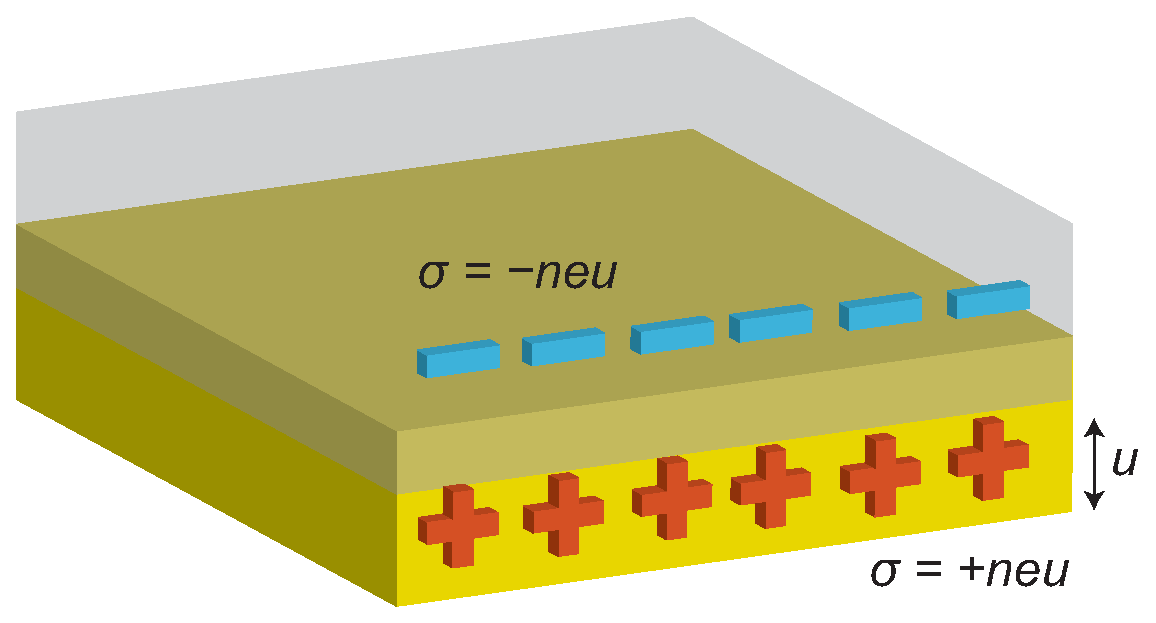
\includegraphics[scale=0.5]{THM/bulk.eps}
\caption{\label{fig:bulk}Longitudinal collective oscillations of the conduction electrons of a metal (Volume plasmons)}
\end{figure}
 We can derive plasma frequency $\omega_p$ from the simple harmonics oscillation model, a collective displacement of the electron cloud by a distance $u$ leads to a surface charge density $\sigma = \pm neu$ at the slab boundaries. This establishes a homogeneous electric field $\mathbf{E} = \frac{neu}{\varepsilon_0}$ inside the slab. Thus, the displaced electrons experience a restoring force, and their movement can be described by the equation of motion $nm\ddot{u} = -ne\mathbf{E}$. Inserting the expression for the electric field, this leads to
 \begin{subequations}
 \begin{align}
 nm\ddot{u} = -\frac{n^2e^2u}{\varepsilon_0} \\
 \ddot{u} + {\omega_p}^{2}u = 0\text{.}
 \end{align}
 \end{subequations}
  The plasma frequency $\omega_p = \sqrt{\frac{ne^2}{\varepsilon_0m}}$ can thus be recognized as the natural frequency of a free oscillation of the electron sea. The quanta of these charge oscillations are called plasmons. Due to the longitudinal nature of the excitation, volume plasmons do not couple to transverse electromagnetic waves, and can only be excited by particle impact. We can derive the dispersion relation of the generalization of volume plasmons, traveling plasma waves, from curl electric field equations (Equations~\ref{eq:curlE})
 \begin{subequations}
 \begin{align}
 \curl{\curl \mathbf{E}} &= -\mu_0 \frac{\partial^2\mathbf{D}}{\partial t^2}\label{eq:curlE}\\
\mathbf{K}( \mathbf{K}\cdot \mathbf{E}-K^{ 2 }\mathbf{E} ) &=-\varepsilon ( \mathbf{K},\omega  ) \frac { { \omega  }^{ 2 } }{ { c }^{ 2 } } \mathbf{E}
 \end{align}
 \end{subequations}  
and plasma model, and a simple equation of motion for an electron of the plasma subjected to an external electric field $\mathbf{E}$
 \begin{equation}
m\ddot{\mathbf{x}} + m\gamma\dot{\mathbf{x}} = -e\mathbf{E}\text{.}
\end{equation}
Assuming a harmonic time dependence $\mathbf{E}( t )=\mathbf{E}_0\mathrm{e}^{-i\omega t}$ of the driving field, a particular solution of this equation describing the oscillation of the electron is $\mathbf{x} ( t ) = \mathbf{x}_0 \mathrm{e}^{-i\omega t} $. The complex amplitude $\mathbf{x}_0$ incorporates any phase shifts between driving field and response via
\begin{equation}
\mathbf{x} ( t ) = \frac{e}{m( \omega^2 + i\gamma\omega )}\mathbf{E}( t )\text{.}
\end{equation}
The displaced electrons contribute to the macroscopic polarization
\begin{equation}
\mathbf{P}=-\frac{ne^2}{m( \omega^2 + i\gamma\omega )}\mathbf{E}( t )\text{.}
\end{equation}
Inserting $\mathbf{P}$ into dielectric displacement field equation $\mathbf{D} = \varepsilon_0\mathbf{E} + \mathbf{P}$ yields
\begin{equation}
\mathbf{D} = \varepsilon_0(1-\frac{\omega_p^2}{\omega^2 + i\gamma\omega})\mathbf{E}\text{,}
\end{equation}
where $\omega_p^2 = \frac{ne^2}{\varepsilon_0m}$. Therefore, the dielectric function of the free electron gas
\begin{equation}
\varepsilon(\omega) = 1- \frac{\omega_p^2}{\omega^2 + i\gamma\omega}\text{.}\label{eq:dielefu}
\end{equation}
We arrive at the desired result by using equation~\ref{eq:dielefu} and the generic dispersion relation $K^2=\varepsilon(\mathbf{K},\omega)\frac{\omega^2}{c^2}$, the dispersion relation of traveling waves becomes
\begin{equation}
\omega^2 = \omega_p^2 + \mathbf{K}^2c^2\text{.}
\end{equation}
From this relation, we can figure out the oscillation properties in any frequency of external field. Note that this branch can not confine the electromagnetic waves, it would radiate out the energy, so this mode is also called radiative surface plasmon.

\section{Surface plasmon polaritons at interface between dielectric and metal}

Surface plasmon polaritons (SPPs) are eigenmodes of transverse magnetic (TM) waves, which coupling the electromagnetic fields to oscillations of the conductor's electron plasma, propagate at a interface between dielectric and metal, and are confined in perpendicular direction. Providing a flat interface between dielectric and metal half-spaces with dielectric constants $\varepsilon_d$ and $\varepsilon_m$ , respectively, and assuming the interface normal to z direction and the SPPs propagate along the $x$ direction, the SPP wave vector $\beta$ is related to the frequency $\omega$ through the dispersion relation
\begin{equation}
\beta = k_0\sqrt{\frac{\varepsilon_d\varepsilon_m}{\varepsilon_d + \varepsilon_m}}\text{,}\label{eq:sppsdisp}
\end{equation}
where $k_0 = \omega/c$ is the free-space wave vector. We take $\omega$ to be real and allow $\beta$ to be complex.

The optical response of metals is often described by the Drude model for a free-electron gas~\cite{kittel1976introduction},
\begin{equation}
\varepsilon_{Drude}(\omega)=1-\frac{\omega_p^2}{\omega^2+i\Gamma\omega}\text{,}
\end{equation}
in which $\Gamma$ is a damping rate due to electron-electron and electron-phonon scattering.
Figure~\ref{fig:SPPdisp} shows the dispersion curve~\ref{eq:sppsdisp} with Drude metal  in the absence of losses ($\Gamma=0$) for air ($\varepsilon_d = 1$) and fused silica ($\varepsilon_d = 2.25$) interface.
\begin{figure}[htb]
\centering
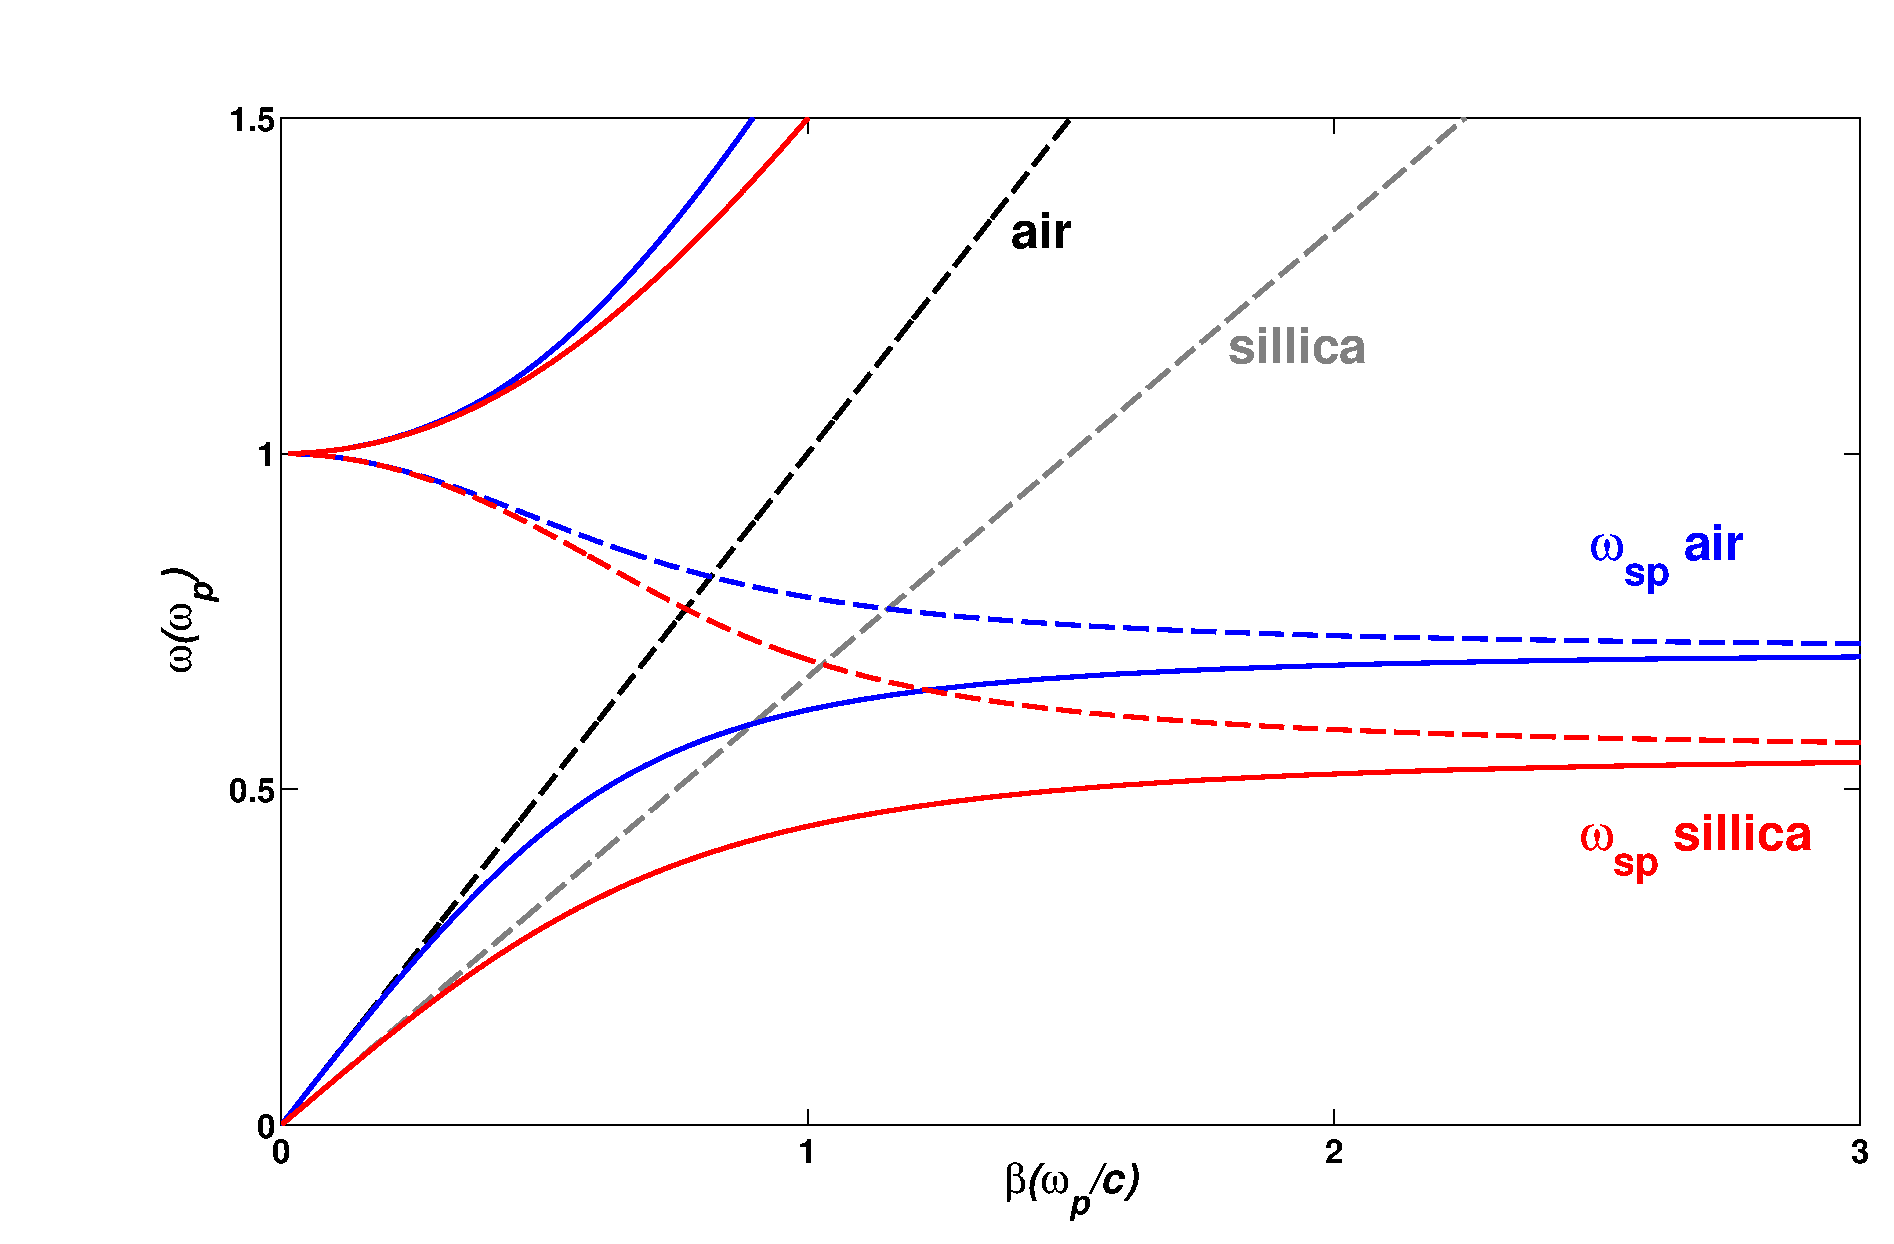
\includegraphics[scale=0.4]{THM/SPPdisp.eps}
\caption{\label{fig:SPPdisp}Dispersion relation of SPPs at the interface between a Drude metal with negligible collision frequency and air (blue curves) and silica (red curves).}
\end{figure}
For small wave vectors SPPs propagation constant $\beta$ is close to $k_0$ at the light line, in the opposite regime of the frequency close to surface plasmon frequency $\omega_p$. It also shows that the SPPs line lying to the right of the respective light lines of air and silica, so that SPPs are directed by light due to phase mismatching. The wave vector mismatch between SPPs and radiation modes needs to be overcome in order to excite or detect SPPs. This can be achieved by multiple methods~\cite{raether1988surface}. In the Otto configuration, light in a prism that is brought in close vicinity to a metal surface can excite SPPs through coupling to the evanescent field. Because light in the prism has a larger wave vector than that in air, it can be phase-matched to the SPPs. In the related Kretschmann-Raether geometry, coupling to SPPs occurs through a metal film that is deposited on a prism. In the grating coupling configuration, metal surface with a shallow grating of grooves or holes with lattice constant $a$. For the simple 1D grating of grooves depicted in Figure~\ref{fig:grating},
\begin{figure}[htb]
\centering
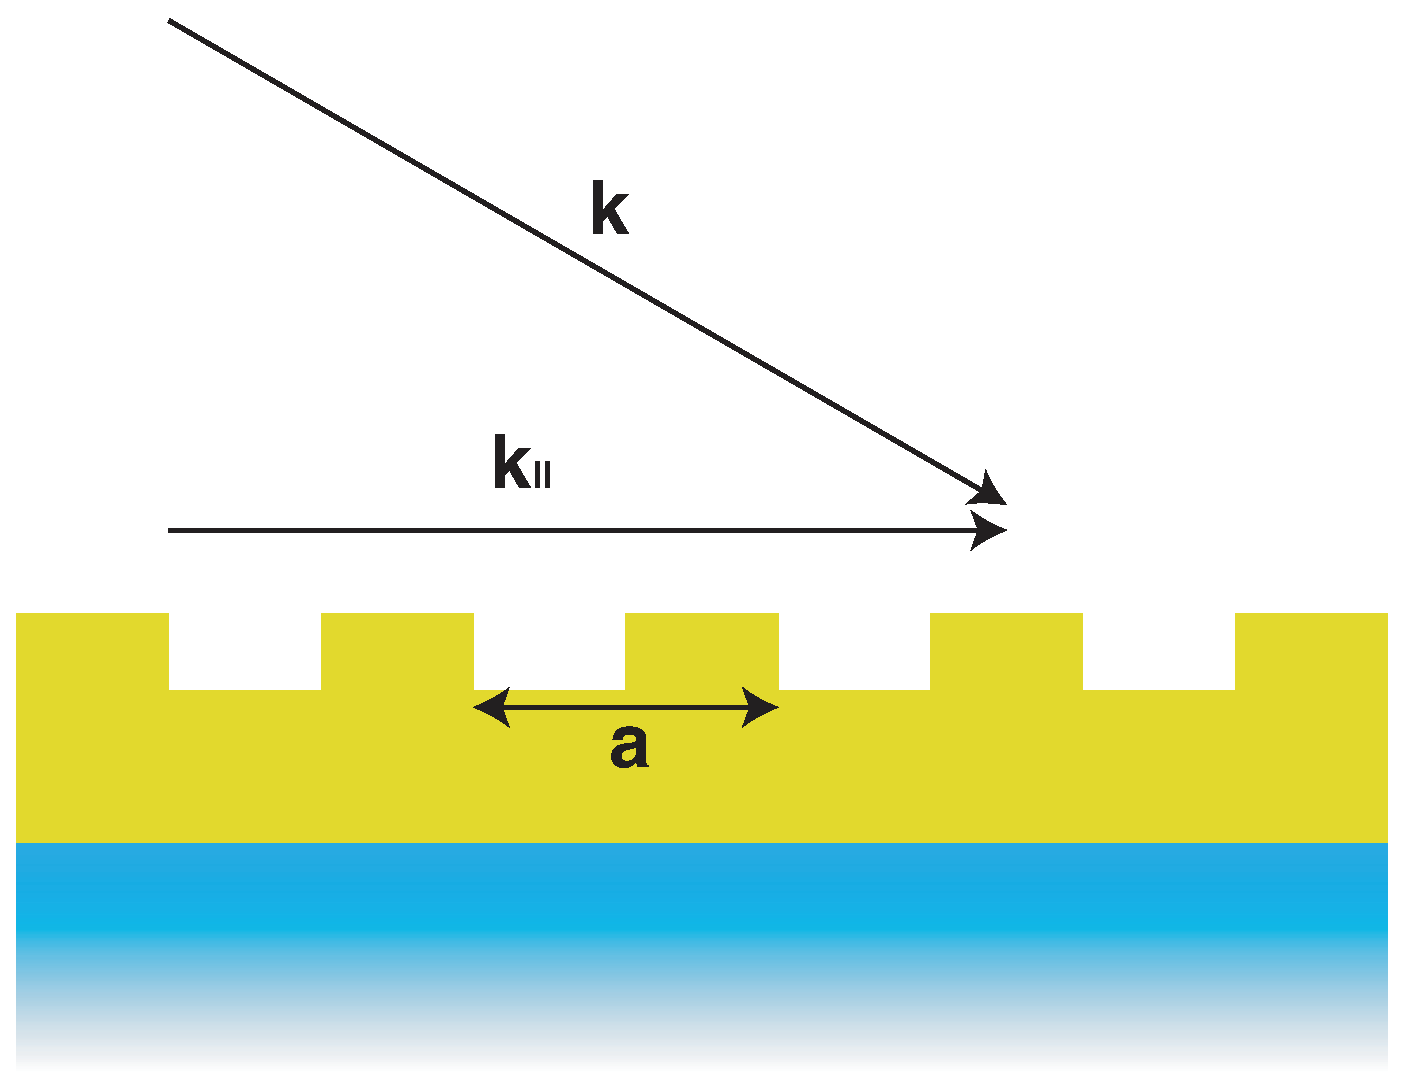
\includegraphics[scale=0.5]{THM/grating.eps}
\caption{\label{fig:grating}Phase-matching of light to SPPs the grating coupling configuration.}
\end{figure}
phase-matching takes place when the condition is fulfilled
\begin{equation}
\beta = k_0 \sin{\theta} \pm \nu g\text{,}
\end{equation}
where $g=\frac{2\pi}{a}$ is the reciprocal vector of the grating, and $\nu=(1,2,3\dots)$.
As with prism coupling, excitation of SPPs is detected as a minimum in the reflected light. The reverse process can also take place, SPPs propagating along a surface modulated with a grating can couple to light and thus radiate. 

%\bibliographystyle{unsrt}
%\bibliography{thesisbib}
%\chapter{Experiment}
\label{c:exp}

\section{Atomic force microscopy}

\begin{figure}[htb]
\centering
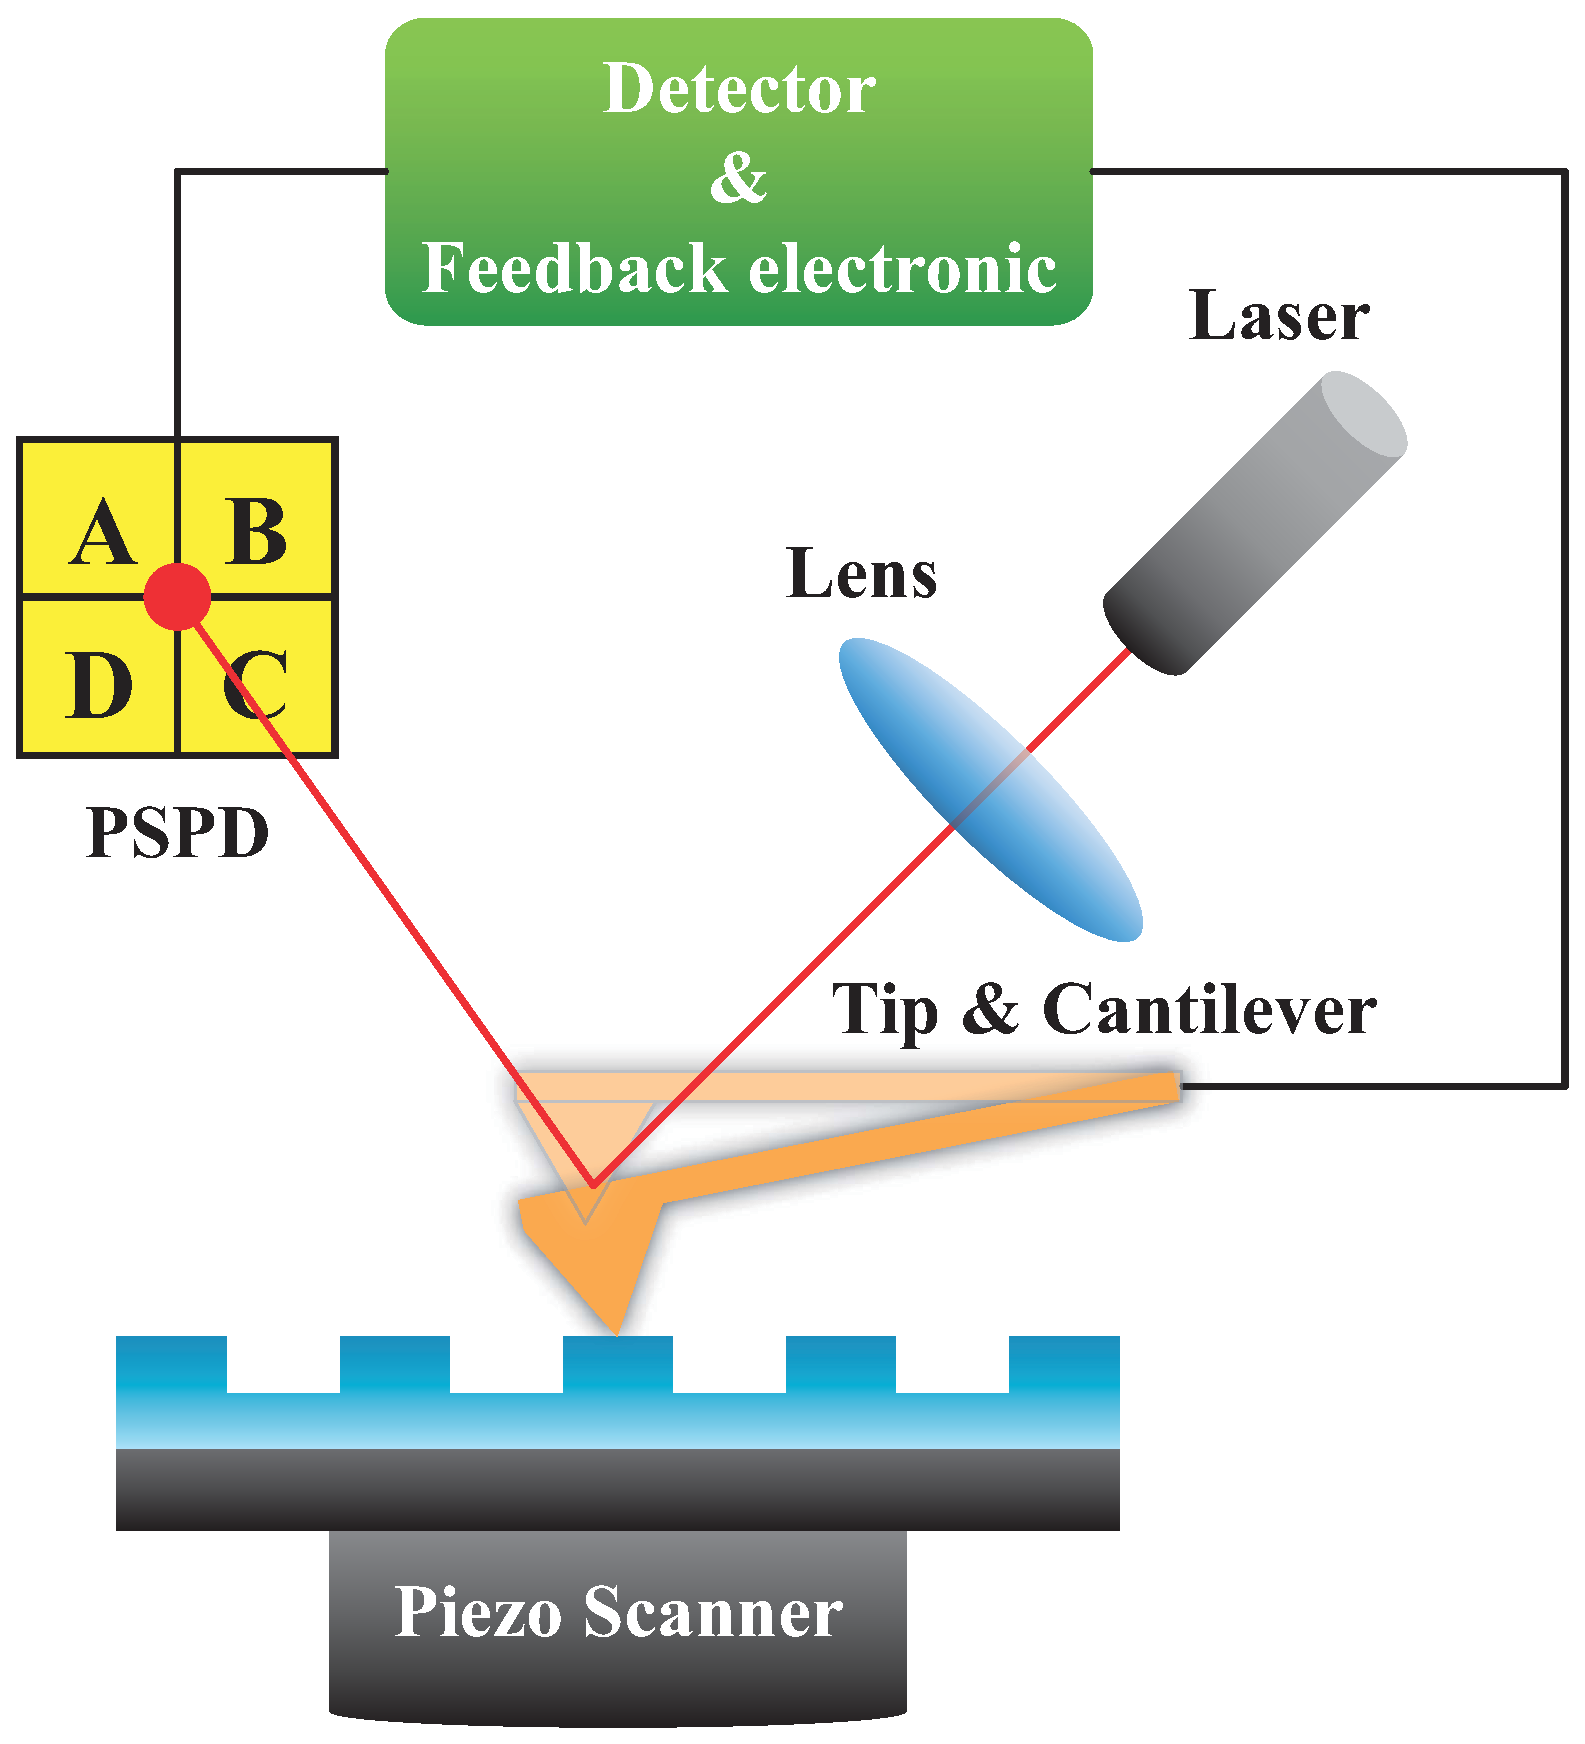
\includegraphics[scale=0.35]{EXP/afm1.eps}
\caption{\label{fig:afm1}Schematic of atomic force microscopy.}
\end{figure}
Atomic force microscope (AFM) is a type of scanning probe microscopes (SPM)~\cite{bennig1988atomic}.  The schematic of AFM is shown in Figure~\ref{fig:afm1}. AFM operates by measuring force between a probe and the specimen surfaces. In general,  the probe is a sharp tip at a cantilever's end. The cantilever can be deflected by atomic forces to sufficiently large amount, then AFM can measure the vertical and lateral deflections of the cantilever by using the optical system. A laser beam is transmitted to cantilever, and the reflected laser beam is detected with a position-sensitive photo detector (PSPD). PSPD is four-sectional that allows measuring not only vertical but lateral bending too(Figure~\ref{fig:afm2}). The output of the PSPD is provided to a computer for processing of the data for providing a topographical image of the surface with atomic resolution, and controlling the height between probe and specimen surfaces by applying voltage on piezoelectric scanner.
\begin{figure}[htb]
\centering
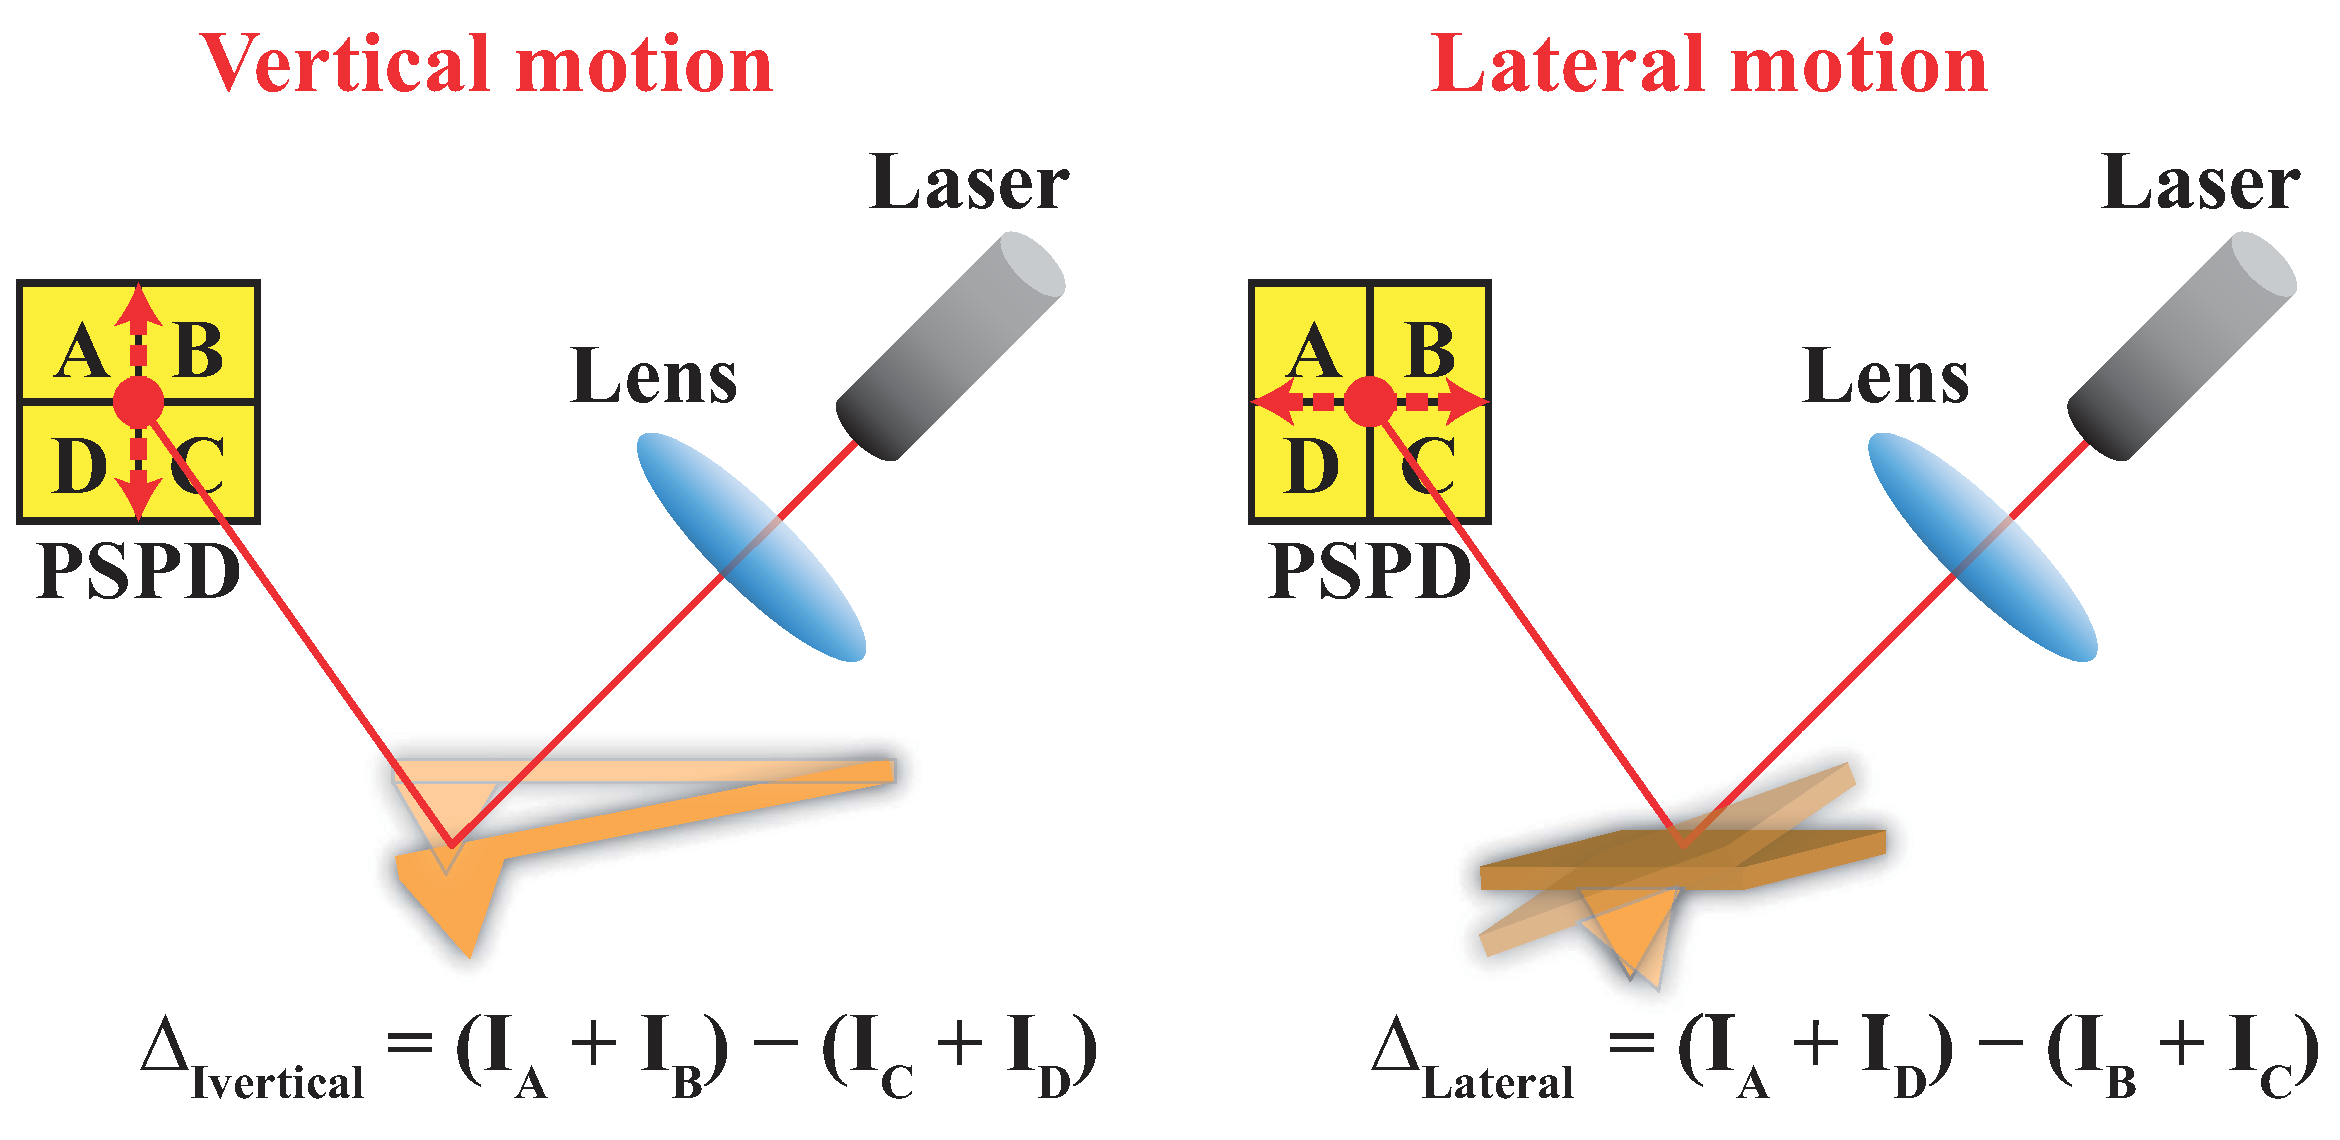
\includegraphics[scale=0.4]{EXP/afm2.eps}
\caption{\label{fig:afm2}Schematic of optical system for cantilever deflections detection.}
\end{figure}

The physical principle of the AFM operation is based on interaction between the probe tip and the specimen surface(Figure~\ref{fig:afm3}). When the cantilever approaches the specimen surface, Van der Waals forces start acting upon it . They are sufficiently far-ranging and are felt at the distance of a few tens of angstroms. Then at the distance of several angstroms repulsive force starts acting. In humid air a water layer is present on the specimen surface. The capillary force arises that holds the tip in contact with the surface and increases the minimum achievable interaction force. Electrostatic interaction between the probe and the sample may appear rather often. This can be both attraction and repulsion. Van der Waals attraction forces, capillary, electrostatic and repulsion forces at the point where the tip touches the sample and forces acting upon the tip from the deformed cantilever compensate each other in equilibrium. Based on the type and degree of this interaction the AFM modes can be broken down into contact and semi-contact(Figure~\ref{fig:afm3} ), which is a transition mode between the contact and non-contact modes.
\begin{figure}[htb]
\centering
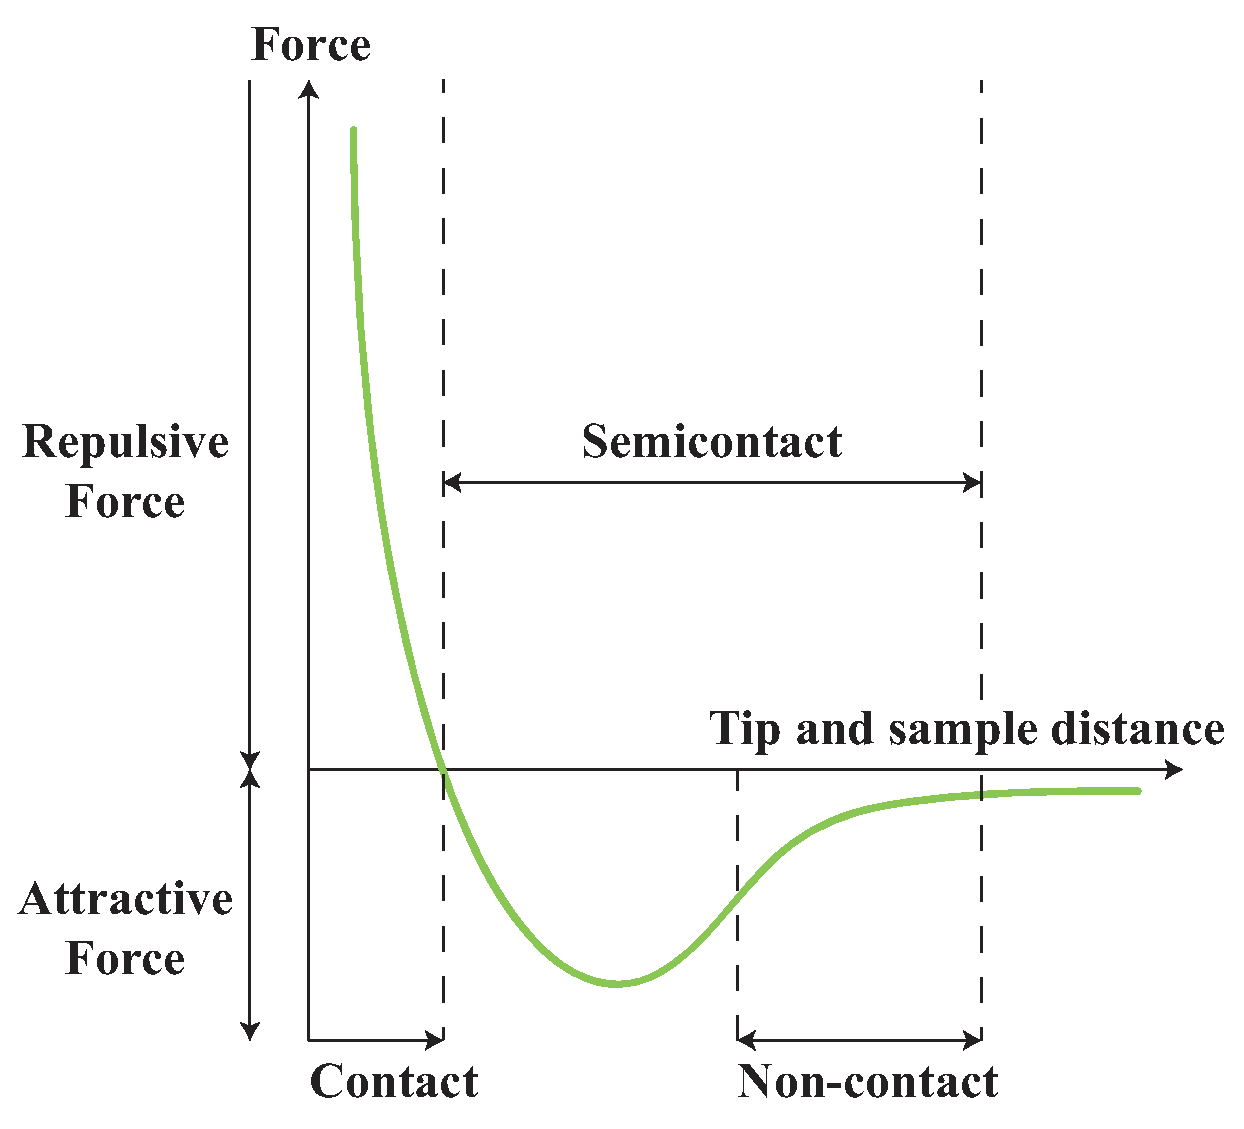
\includegraphics[scale=0.6]{EXP/afm3.eps}
\caption{\label{fig:afm3}Sketch of tip-sample forces.}
\end{figure}

\paragraph{Contact mode}

In contact mode of operation the cantilever deflection under scanning reflects repulsive force acting upon the tip. Repulsion force $\mathbf{F}$ acting upon the tip is related to the cantilever deflection value $\mathbf{x}$ under Hooke's law: $\mathbf{F}=-K \cdot  \mathbf{x}$, where $K$ is cantilever spring constant. The spring constant values for different cantilevers usually vary from 0.01 to several $\mathbf{N/m}$.

In our units the vertical cantilever deflection value is measured by means of the optical registration system and converted into electrical signal DFL (difference signal between the upper and lower halves of the PSPD) . In contact mode the DFL signal is used as a parameter characterizing the interaction force between the tip and the surface. There is a linear relationship between the DFL value and the force. In constant force mode of operation the deflection of the cantilever is maintained by the feedback circuitry on the preset value. So vertical displacement of the scanner under scanning reflects topography of sample under investigation.

Contact force microscopy is surface topography measurement in the contact mode.The microscope operation in the mode of maintaining constant interaction force between the tip and the surface sample, and is the base for measuring surface topography as well as for measuring local rigidity, local viscosity and local friction force. Constant force mode has some advantages and disadvantages. Main advantage of constant force mode is possible to measure with high resolution simultaneously with topography and some other characteristics, such as friction forces, spreading resistance etc. Constant force mode has also some disadvantages. Speed of scanning is restricted by the response time of feedback system. When exploring soft samples they can be destroyed by the scratching because the probe scanning tip is in direct contact with the surface. Therefore, under scanning soft unhomogeneous samples the local flexure of sample surface varies. As a result acquired topography of the sample can be proved distorted. Possible existence of substantial capillary forces imposed by a liquid adsorption layer can decrease the resolution.

\paragraph{Semi-contact mode}

The semi-contac mode can be characterized by some advantages in comparison with contact mode. First of all, in this mode the force of pressure of the cantilever onto the surface is less, that allows to work with softer materials such as polymers and bio-organics. The semi contact mode is also more sensitive to the interaction with the surface that gives a possibility to investigate some characteristics of the surface distribution of magnetic and electric domains, elasticity and viscosity of the surface. 

Widely used semi-contact mode has some disadvantage concerned with the usage of the feedback circuit. The scanning speed in semi-contact mode is restricted by the feedback circuit reaction time. This disadvantage can be overcome by the fact that under scanning new value of cantilever oscillation amplitude (and error signal) usually is achieved faster than preset value of the cantilever oscillation amplitude can be reached by the feedback system. Time of the reaching new value of the oscillation amplitude is determined by the oscillation period and Q-quality of the cantilever.
The feedback error signal, emerging when scanning in the semi-contact mode, contains some additional information about the topography. It can be utilized for achieving a more precise recovery of the relief. 

Additionally, similarly to the contact error mode, which can be considered as intermediate between the constant force mode and constant height mode, the feedback gain factor (i.e. the feedback processing speed) can be adjusted for the system to be able to trace subtle changes of the relief and to be too slow to trace the steep changes. Then, when the probe travels over minor irregularities, scanning will be carried out with an almost constant piezo scanner length. As a result, the slow changes of the relief will hardly show up on the images, and the steep changes will appear in high contrast. This may be helpful in finding minor irregularities on large areas against major sloping relief features. It must be noted that height of the minor irregularities must be less than amplitude of cantilever oscillation.

\section{Scanning electron microscopy}

The scanning electron microscope (SEM) is used for the observation of specimen surfaces~\cite{von1938elektronen}. When the specimen is irradiated with a fine electron beam, secondary electrons are emitted from the specimen surface. Topography of the surface can be observed by two-dimensional scanning of the electron probe over the surface and acquisition of an image from the detected secondary electrons. The concept schematic of commercial SEM (JEOL, JSM-6500F) is shown in Figure~\ref{fig:sem1}. The basic unit is composed of an electron optical system, a specimen stage, a secondary-electron detector, an image display unit, and an operation system. The electron optical system consists of an electron gun, a condenser lens and an objective lens to produce an electron probe, a scanning coil to scan the electron probe, and other components. The system inside of the microscope column are kept at vacuum.
\begin{figure}[htb]
\centering
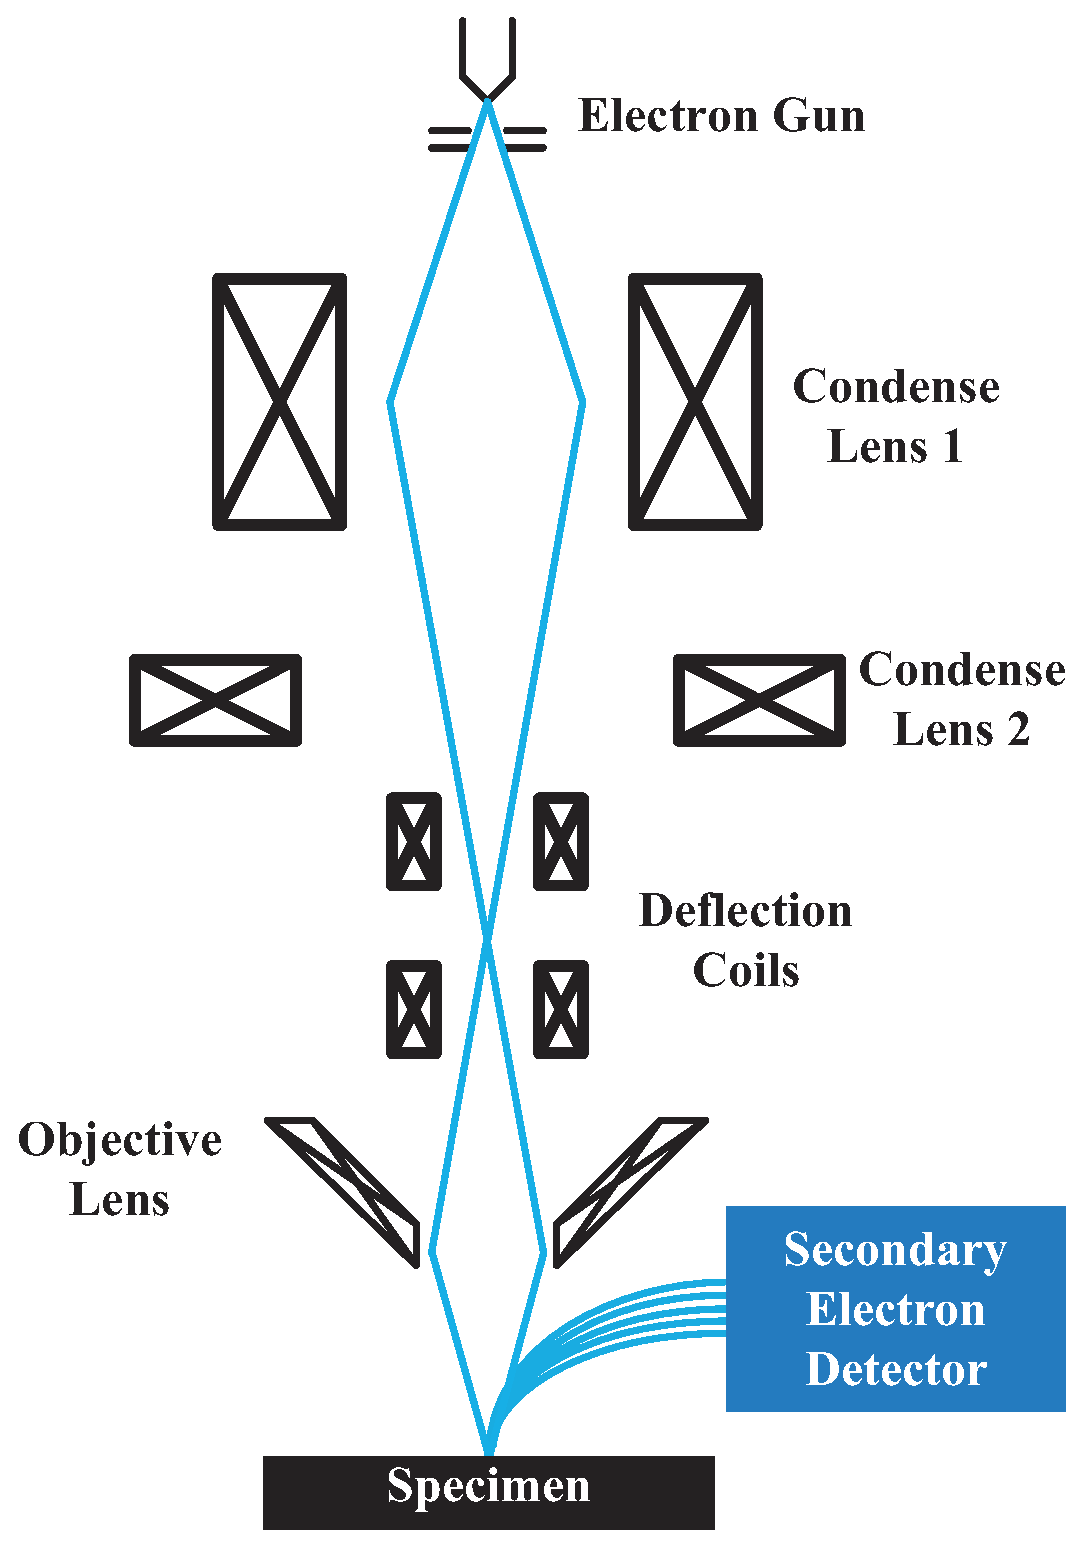
\includegraphics[scale=0.5]{EXP/SEM.eps}
\caption{\label{fig:sem1}Basic construction of a scanning electron microscopy.}
\end{figure}


The JSM-6500F utilizes a Schottky type field-emission (T-FE) gun for the electron source. The T-FE gun can constantly supply the surface of the cathode with zirconium oxide by heating the surface of cathode to 1800 K. For this reason, it can easily obtain stable and high probe current (range from several pA to 100 nA) compared with the traditional thermal emission electron gun and cold field-emission gun.

The magnetic condenser and objective lens system act to control the diameter of the beam as well as to focus the beam on the specimen due to a rotationally-symmetric magnetic field is formed when we pass a direct electric current through a coilwound electric wire in the magnetic lens. A pair of deflector coils, which between the condenser and objective lens, controlled by the scan generator, which are responsible for rastering that focused beam across the specimen surface. The size of the rastering pattern is under magnification control. The beam is rastered from left to right and top to bottom. There is a one-to-one correspondence between the rastering pattern on the specimen and the rastering pattern used to produce the image on the monitor. The resolution we choose to image at will obviously affect the number of pixels per row as well as the number of rows that constitute the scanned area.

The signal is generated from the specimen, and collected by the detector and subsequently processed to generate the image. That processing takes the intensity of the signal coming from a pixel on the specimen and converts it to a grayscale value of the corresponding monitor pixel. The monitor image is a two dimensional rastered pattern of grayscale values.

With the beam focused on the specimen surface, all we need to do to change magnification is to change the size of the rastered area on the specimen. The size of the monitor raster pattern is constant. Magnification will increase if we reduce the size of the area scanned on the specimen.

%\bibliographystyle{unsrt}
%\bibliography{thesisbib}
%\include{main}
%\chapter{Conclusions}
\label{c:conclusions}



\backmatter

%---------- Input your reference here ---------
\bibliographystyle{unsrt}
\addcontentsline{toc}{chapter}{\bibname}
\bibliography{thesisbib}

%----------- Input your appendix here  -----------
%\input{appendixA}

\end{document}
